\documentclass[a4paper]{report}
\usepackage{tocloft}
\renewcommand{\cftchapleader}{\cftdotfill{\cftdotsep}} 

\usepackage{enumitem}
\usepackage{titling}
\usepackage{listings}
\usepackage{url}
\usepackage{soul}
\usepackage{hyperref}
\usepackage{setspace}
\usepackage{subfig}
\usepackage{sectsty}
\usepackage{pdfpages}
\usepackage{colortbl}
\usepackage{multirow}
\usepackage{multicol}
\usepackage{relsize}
\usepackage{amsmath}
\usepackage{wasysym}
\usepackage{fancyvrb}
\usepackage[yyyymmdd]{datetime}
\usepackage{amsmath,amssymb,amsthm,graphicx,xspace}
\usepackage[titlenotnumbered,noend,noline]{algorithm2e}
\usepackage[compact]{titlesec}
\usepackage{XCharter}
\usepackage[T1]{fontenc}
\usepackage[scaled]{beramono}
\usepackage[normalem]{ulem}
\usepackage{booktabs}
\usepackage{tikz}
\usetikzlibrary{arrows,automata,shapes,trees,matrix,chains,scopes,positioning,calc,decorations.pathreplacing}
\tikzstyle{block} = [rectangle, draw, fill=blue!20, 
    text width=2.5em, text centered, rounded corners, minimum height=2em]
\tikzstyle{bw} = [rectangle, draw, fill=blue!20, 
    text width=4em, text centered, rounded corners, minimum height=2em]

\definecolor{namerow}{cmyk}{.40,.40,.40,.40}
\definecolor{namecol}{cmyk}{.40,.40,.40,.40}
\renewcommand{\dateseparator}{-}

\let\LaTeXtitle\title
\renewcommand{\title}[1]{\LaTeXtitle{\textsf{#1}}}

\lstset{basicstyle=\footnotesize\ttfamily,breaklines=true}

\newcommand{\CPP}{C\nolinebreak\hspace{-.05em}\raisebox{.4ex}{\tiny\bf +}\nolinebreak\hspace{-.10em}\raisebox{.4ex}{\tiny\bf +}}
\def\CPP{{C\nolinebreak[4]\hspace{-.05em}\raisebox{.4ex}{\tiny\bf ++}}}

\newcommand{\handout}[5]{
  \noindent
  \begin{center}
  \framebox{
    \vbox{
      \hbox to 5.78in { {\bf ECE459: Programming for Performance } \hfill #2 }
      \vspace{4mm}
      \hbox to 5.78in { {\Large \hfill #4  \hfill} }
      \vspace{2mm}
      \hbox to 5.78in { {\em #3 \hfill \today} }
    }
  }
  \end{center}
  \vspace*{4mm}
}

\newcommand{\lecture}[3]{\handout{#1}{#2}{#3}{Lecture #1}}
\newcommand{\tuple}[1]{\ensuremath{\left\langle #1 \right\rangle}\xspace}

\addtolength{\oddsidemargin}{-1.000in}
\addtolength{\evensidemargin}{-0.500in}
\addtolength{\textwidth}{2.0in}
\addtolength{\topmargin}{-1.000in}
\addtolength{\textheight}{1.75in}
\addtolength{\parskip}{\baselineskip}
\setlength{\parindent}{0in}
\renewcommand{\baselinestretch}{1.5}
\newcommand{\term}{Winter 2019}

\singlespace



\begin{document}

\tableofcontents


\chapter*{1 --- Programming for Performance}

\addcontentsline{toc}{chapter}{1 --- Programming for Performance}

\section*{Performance!}
By this point, I'm certain you know what ``programming'' means, but we need to take a minute right off the top to define ``performance''. This course is not about how to program when other people are watching (fun as that can be, as the popularity of Hackathons shows). What it's really about is making a program ``fast''. Alright, but what does it mean for a program to be fast?

Let's think about the program execution as completion of some number of items -- things to do. We have two concepts: items per unit time (bandwidth -- more is better), and time per item (latency -- less is better). Improving on either of these will make your program ``faster'' in some sense. In a way they are somewhat related: if we reduce the time per item from 5~s to 4~s it means an increase of 12 items per minute to 15 items per minute... if the conditions are right. Hopefully we could improve both metrics, but sometimes we'll have to pick one.

\paragraph{Items per unit time.} This measures how much work can get 
done simultaneously; we refer to it as bandwidth.
Parallelization -- or doing many things at once -- improves the number
of items per unit time. We might measure items per time in terms of
transactions per second or jobs per hour. You might still have to wait
a long time to get the result of any particular job, even in a
high-bandwidth situation; sending a truck full of hard drives across
the continent is high-bandwidth but also high-latency.

\paragraph{Time per item.} This measures how much time it takes to do
any one particular task: we can call this the latency or response time.
It doesn't tend to get measured as often as bandwidth, but it's especially
important for tasks where people are involved. Google cares a lot about
latency, which is why they provide the {\tt 8.8.8.8} DNS servers.
(Aside: when dealing with users, 100ms is the maximum latency for
systems that purport to respond instantaneously~\cite{nielsen93:_respon_times}.)

\paragraph{Examples.} Say you need to make
100 paper airplanes. What's the fastest way of doing this?

\vspace*{7em}
% get 100 friends to fold 1 airplane each: that's the 
% embarassingly parallel aspect of this problem
% what about further parallelization? You could use an assembly line
% to pipeline the task, but you then have to transport the airplane
% between people
% or, you can fold the planes faster by setting up the workstation
% optimally

Here's another example, containing various communications technologies:

\begin{center}
\begin{tikzpicture}
  \draw (-6,0) -- (6,0) node[below right,xshift=-4em] {high latency};
  \draw (0,-1.5) -- (0,1.5) node[right] {high bandwidth};
\end{tikzpicture}
\end{center}
% fiber: top left
% DSL: below fiber
% cable: to the right of DSL
% satellite internet: way right of cable

% shipping hard drives on a train is top right
% sending postcards is bottom right
% SMS is middle of lower left quadrant
% morse code?

We will focus on completing the items (doing useful work), not on transmitting information, but the above example makes the difference between bandwidth and latency clear.

\section*{Improving Latency}
Although we'll mostly focus on parallelism in this course, a
good way of writing faster code is by improving single-threaded 
performance. Unfortunately, there will be a limit to how much you can
improve single-threaded performance; however, any improvements here
may also help with the parallelized version. On the other hand, faster
sequential algorithms may not parallelize as well. But let's take a look at some
ways you can improve latency.

\paragraph{Profile the code.} You can't successfully make your code 
faster if you don't know why it's slow. Intuition seems to often be
wrong here, so run your program with realistic workloads under a profiling
tool and figure out where all the time is going. This is a specific instance of one of my favourite rules of engineering: ``Don't guess; measure''. 

Let's take a quick minute to visit \url{http://computers-are-fast.github.io/} and take a quiz on how fast computers can do certain operations~\cite{cafgithub}. Are the results surprising to you? Did you do really well or really badly? Chances are that you got some right and some wrong... and the ones that were wrong were not just a little wrong, but off by several orders of magnitude. Moral of the story is: don't just guess at what the slow parts of your code are. It's okay to have a theory as a starting point, but test your theory.


\paragraph{Do less work.} A surefire way to be faster is to omit unnecessary
work. Two (related) ways of omitting work are to avoid calculating
intermediate results that you don't actually need; and computing
results to only the accuracy that you need in the final output.

Interesting to note: producing text output to a log file or to a console screen is surprisingly expensive for the computer. Sometimes one of the best ways to avoid unnecessary work is to spend less time logging and reporting. It might make debugging harder, yes, but once the code is correct (or close enough), removing the logging and debugging statements can actually make a difference. Especially in a multithreaded context, logging and debugging often incur synchronization cost.

A hybrid between ``do less work'' and ``be smarter'' is caching, where
you store the results of expensive, side-effect-free, operations
(potentially I/O and computation) and reuse them as long as you
know that they are still valid. Caching is really important in certain situations.

\paragraph{Be prepared.} If you know something that the user is going to ask for in advance, you can have it at the ready to provide upon request. Example from that other job of mine [JZ]: users often want an Excel export of various statistics on their customs declarations. If the user asks for the report, generating it takes a while, and it means a long wait. If, however, the report data is pre-generated and stored in the database (and updated as necessary) then putting it in the Excel output file is simple and the report is available quickly.

\paragraph{Be smarter.} You can also use a better algorithm. This is probably ``low hanging fruit'' and by the time it's time for P4P techniques this has already been done. But if your sorting algorithm is $\Theta(n^{3})$ and you can replace it with one that is $\Theta(n^{2})$, it's a tremendous improvement even there are yet better algorithms out there. An improved algorithm includes better asymptotic performance
as well as smarter data structures and smaller constant factors.
Compiler optimizations (which we'll discuss in this course) help with
getting smaller constant factors, as does being aware of the cache
and data locality/density issues.

Sometimes you can find this type of improvements in your choice of
libraries: you might use a more specialized library which does the
task you need more quickly. The build structure can also help, i.e. which parts of the code are in libraries and which are in the main executable. It's a hard decision sometimes: libraries may be better and more reliable than the code you can write yourself. Or it might be better to write your own implementation that is optimized especially for your use case.

\paragraph{Improve the hardware.} Once upon a time, it was okay to write code with terrible performance on the theory that next year's CPUs would make it acceptably, and spending a ton of time optimizing your code to run on today's processors was a waste of time. Well, those days seem to be over; CPUs are not getting much faster these days (evolutionary rather than revolutionary change). But sometimes the CPU is not the limiting factor: your code might be I/O-bound, so you might be able
to improve things dramatically by going to solid-state drives or non-volatile memory (e.g. Optane/3DXpoint); or you might be swapping
out to disk, which kills performance (add RAM). Profiling is key here, to find out what the slow parts of execution are. When it comes down to it, spending a few thousand dollars on better hardware is often much cheaper than paying programmers to spend their time to optimize the code. (Programmers are super expensive.)

\paragraph{On using assembly.} Not that long ago, compilers were not very smart and expert programmers could outsmart the compiler and produce better assembly by hand. This tends to be a bad idea these days. Compilers are going to be better at generating assembly than you are. Furthermore, CPUs may accept the commands in x86 assembly (or whatever your platform is) but internally they don't operate on those commands directly; they rearrange and reinterpret and do their own thing. Still, it's important to understand what the compiler is doing, and why it can't optimize certain things (we'll discuss that), but you don't need to do it yourself. However, giving hints to the compiler about e.g. vector instructions can be helpful.

\paragraph{Anecdote time.} Recently I [JZ] was presented with a ticket that read as follows: ``the report generation has been running for three hours; I think it's stuck.'' Turns out the report had not been running for that long, it reached a 30 minute time limit and the server had killed the task (and it just looked like it was running). So now I have a puzzle: how do I speed up this task to get it under the 30 minute time limit?

How does the report work? It selects the transactions for a given period from the database. Then for each transaction, it looks up the latest article data, recomputes the transaction's worth based on the most up to date currency exchange rate, and then stores the updated transaction in the database again.

Step one was to bring up the profiler and look at a few things. The slow steps were primarily database operations: retrieving of exchange rates, retrieving the article data, and then storing all the transactions. Right, with this data, it's time to apply some strategies here.

Caching played a big role: the exchange rate data doesn't change for the report (it is run retroactively, with a date on the end of the last month, so the exchange rates are defined for that day rather than floating). So retrieving the exchange rate 500 times can be cut down to once per currency. Caching was also important for the articles; an article might be used dozens of times, so loading it from the database repeatedly is also a waste of time. Also, I could select all the articles at once rather than each one as encountered.

How about doing less work? For one thing, instead of pulling all the fields of the article from the database, why not just get the five that are actually needed? And in saving the transactions, what if we only update the parts that changed rather than update the full transaction and all its parts. 

Ultimately, these techniques combined brought the report time down under 30 minutes and it can now run to completion. 

\section*{Doing more things at a time} 
Rather than, or in addition to, doing each thing faster, we can do
more things at a time.

\subsection*{Why parallelism?}
While it helps to do each thing faster, there are limits to how fast
you can do each thing. The (rather flat) trend in recent CPU clock
speeds illustrates this point.  Often, it is easier to just throw more
resources at the problem: use a bunch of CPUs at the same time. We
will study how to effectively throw more resources at problems.
In general, parallelism improves bandwidth, but not latency.
Unfortunately, parallelism does complicate your life, as we'll see.

\paragraph{Different kinds of parallelism.} Different problems are amenable
to different sorts of parallelization. For instance, in a web server, we
can easily parallelize simultaneous requests. On the other hand, it's hard
to parallelize a linked list traversal. (Why?)

\paragraph{Pipelining.} A key concept is pipelining. All modern CPUs do this,
but you can do it in your code too. Think of an assembly line: you can split
a task into a set of subtasks and execute these subtasks in parallel.

\paragraph{Hardware.} To get parallelism, we need to have multiple instruction
streams executing simultaneously. We can do this by increasing the
number of CPUs: we can use multicore processors, SMP (symmetric
multiprocessor) systems, or a cluster or machines. We get different
communication latencies with each of these choices.

We can also use more hardware, like vector processing units built into all modern
chips (SIMD) or graphics processing units (GPUs).

\subsection*{Difficulties with using parallelism}
You may have noticed that it is easier to do a project when it's just
you rather than being you and a team. The same applies to code.
Here are some of the issues with parallel code.

First, some domains are ``embarassingly parallel'' and these problems
don't apply to them; for these domains, it's easy to communicate
the problem to all of the processors and to get the answer back, and
the processors don't need to talk to each other to compute. The canonical
example is Monte Carlo integration, where each processor computes the
contribution of a subrange of the integral.

I'll divide the remaining discussion into limitations and complications.

\paragraph{Limitations.} Parallelization is no panacea, even without
the complications that I describe below. Dependencies are the
big problem.

First of all, a task can't start processing until it knows what it
is supposed to process. Coordination overhead is an issue, and if the
problem doesn't have a succinct description, parallelization can be
difficult. Also, the task needs to combine its result with the other
tasks.

``Inherently sequential'' problems are an issue. In a sequential 
program, it's OK if one loop iteration depends on the result of the
previous iteration. However, such formulations prohibit parallelizing
the loop. Sometimes we can find a parallelizable formulation of the loop,
but sometimes we haven't found one yet.

Finally, code often contains a sequential part and a parallelizable
part.  If the sequential part takes too long to execute, then
executing the parallelizable part on even an infinite number of
processors isn't going to speed up the task as a whole. This is
known as Amdahl's Law, and we'll talk about this soon.

\paragraph{Complications.} It's already quite difficult to make sure that
sequential programs work right. Making sure that a parallel program
works right is even more difficult.

The key complication is that there is no longer a total ordering between
program events. Instead, you have a partial ordering: some events $A$
are guaranteed to happen before other events $B$, but many events $X$ 
and $Y$ can occur in either the order $XY$ or $YX$. This makes your code
harder to understand, and complicates testing, because the ordering that
you witness might not be the one causing the problem.

Two specific problems are data races and deadlocks. 
\begin{itemize}
\item A
\emph{data race} occurs when two threads or processes both attempt to
simultaneously access the same data, and at least one of the accesses
is a write. This can lead to nonsensical intermediate states becoming
visible to one of the participants. Avoiding data races requires
coordination between the participants to ensure that intermediate
states never become visible (typically using locks). 
\item A \emph{deadlock}
occurs when none of the threads or processes can make progress on the
task because of a cycle in the resource requests. To avoid a deadlock,
the programmer needs to enforce an ordering in the locks. Or use some other strategies as we have discussed in previous courses.
\end{itemize}

Another complication is stale data. Caches for multicore processors
are particularly difficult to implement because they need to account
for writes by other cores.

\section*{Scalability}

It gets worse. Performance is great, but it's not the only thing we're interested in. We also care about \textit{scalability}: the trend of performance with increasing load. A program generally has a designed load (e.g., we are expecting to handle $x$ transactions per hour). A properly designed program will be able to meet this intended load. If the performance deteriorates rapidly with increasing load (that is, the number of operations to do), we say it is \textit{not scalable} ~\cite{swps}. This is undesirable, of course, and for the most part if we have a good program design it can be fixed. If we have a bad program design, then no amount of programming for performance techniques are going to solve that (``rearranging deck chairs on the Titanic'').

The things we're going to look at in this course are ways to meet $x$ or even raise the value of $x$. Even the most scalable systems have their limits, of course, and while higher is better, nothing is infinite. There's only so much we can do to push it, but chances are we can make some serious progress if we make the effort.

\section*{The Roadmap}
You have a program and you want to make it fast. To understand what's going on we will need some baseline understanding of hardware: architecture, caches, branch prediction. Understanding those will tell you what are the pitfalls that can make your program slow.

An easy way to get a performance boost is parallelizing your program: use threads for a big performance boost, mitigate the risks (with locking) but also do it well. 

Then when that's mined out you can start thinking about speculation and also about trying to speed up your single thread performance. You can think about going to OpenCL if you have the right kind of task for it, but conversion is hard and the overhead is large. 

If you've done all the things that are sure to make improvement it's time to really dig in with the profiling tools to find where and what to focus on next. And when all (reasonable) improvements have been made, then it's time to make your code work using multiple machines, such as with MPI (and apply some queueing theory to find out how many servers you need!).









\chapter*{2 --- A Crash Course in Modern Hardware}

\addcontentsline{toc}{chapter}{2 --- A Crash Course in Modern Hardware}

You know how \url{http://computers-are-fast.github.io/} featured in Lecture 1? It may also feature on your exams. You might want to print out you results and bring them.

\section*{Modern Processors}

It's critical to understand what's going on with the hardware if we want to write good programs. This lecture is based off the talk by Cliff Click~\cite{modern-hardware}.

Remember the classic von Neumann machine architecture. A program is comprised of both instructions and data, both of which are stored in the same memory. A program executes sequentially, one statement at a time, one after another. That is not really how computers work, at least not anymore, but it is an abstraction we still maybe find useful when it comes to algorithm analysis.

Consider this graph of CPU clock speed (frequency) over time from~\cite{cpudb}:

\begin{center}
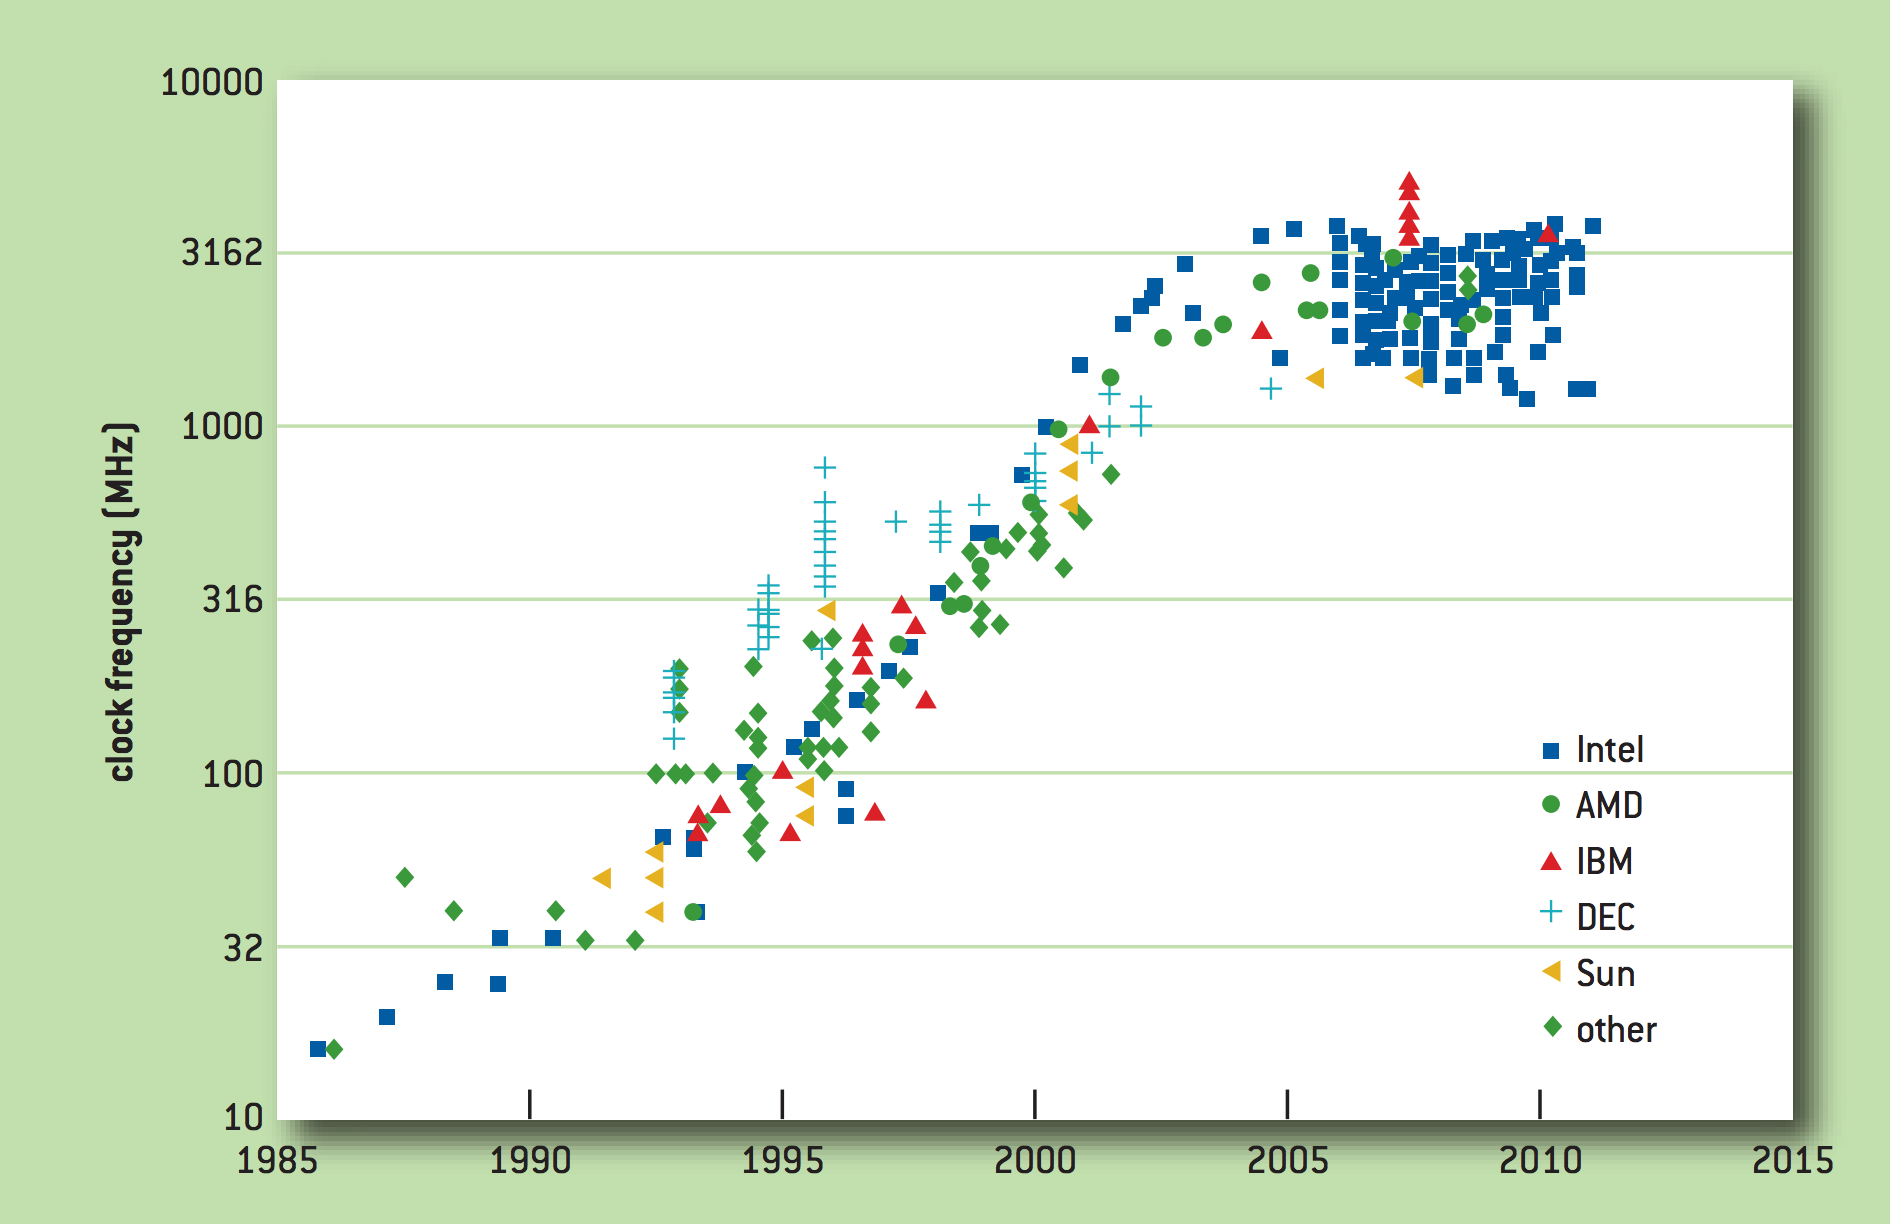
\includegraphics[width=0.7\textwidth]{images/cpu-frequency}
\end{center}

Clearly there is an area in which frequency scaling was effective. Next year's CPU would have a higher clock speed, and higher clock speed means more cycles per second, and more cycles per second means more work is done in a given second, and that means better performance. Except, we hit the wall: clock speeds stop getting faster around 2005, stopping at around 3 GHz. Speeding them up beyond this would take, well, more voltage which means more power and more heat, and more heat means higher failure/error rates, and more cooling, and the cooling takes power too, and all that waste heat, well, it will eventually, at the end of this chain, make polar bears sad.

Digression: if we look at the x86 processor, one with which everyone is probably at least \textit{passingly} familiar, it is a Complex Instruction Set Computing (CISC) processor. In other words, there are a lot of assembly instructions. But why? This was intended for your convenience as a programmer: if you were going to write assembly, wouldn't it be nice to have a sine function that takes one argument instead of having to grind out (or copy-paste) the calculation of a sine routine every single time you needed it? So the hardware people thought they were doing everyone a favour. These are easy to program in, from the way the assembly programmer thinks, but hard to implement and hard to pipeline. 

For a lot of CISC machines, the Cycles Per Instruction (CPI) varied, something like 4-10 cycles to complete any instruction, but at least it was predictable. Every time, no matter what, it takes the same number of cycles. Program performance was basically the number of page faults (disk accesses) times the amount of time it takes to read from disk, plus the instruction execution time (which is generally small compared to page fault service times)\footnote{For further discussion about this, see the ECE~254 notes about page faults and caching and disk read times.}. Thus the optimization goal is: minimize page faults. Page fault count is relatively easy to measure and there are some things we can do to reduce the number of page faults; optimize our data access patterns, change how we pack the data, et cetera. If you were working with an embedded system with no disk (or at least no page faults) then the optimization goal is minimize instruction count.

Between 1990 and 2005 we got some really impressive scaling on CPU frequency. This was caused by a few factors. The first is the advent of the Reduced Instruction Set Computing (RISC) CPU: simpler processors are easier to scale than complex ones, and simpler instructions mean fewer cycles per instruction. That also means we can have more pipelining. The tradeoff is that RISC CPUs are much harder to program in assembly directly, so compilers had to do the work. The example in~\cite{modern-hardware} is delay slots: an instruction after a branch is always executed or worse, the result of a computation is not available to the next instruction. In these cases the ``simple'' solution is to put a \texttt{NOP} (do-nothing) instruction in, good compilers (and programmers) can rearrange instructions, hopefully, to make this work without wasting time. And another thing: memory got cheaper, so we have more of it, so page faults occurred less and less frequently and that's really something.

But then, as we have seen, we hit the (power) wall. And you might think, well, if I run into a wall, I can just go around it. There must be other ways to advance! And there are, except, we hit three other walls too, and now we are surrounded\footnote{``He is intelligent, but not experienced. His pattern indicates two dimensional thinking.'' - Spock, \textit{Star Trek II: The Wrath of Khan}}. What are these other three seemingly-insurmountable barriers?

The first is instruction level parallelism (ILP) is getting close to the limit of what we can do. We can predict branches with a certain accuracy but if we have already got 95\% efficiency, no matter how much time and effort and money is invested into improving the branch prediction routine we get maximally a 5\% increase in branch prediction accuracy which translates into a very small speedup to the execution when we consider just how often a misprediction is the cause of the problem (5\% of 5\% is very small... just making up numbers).

The speed of memory advances has not at all kept up with the advances in CPU technology, so now we have moved from the era of runtime being dominated by page faults to the era of runtime being dominated by cache misses. Adding more cache isn't a perfect solution though, and doubling, say, level one cache (at great expense) does not double the speed of the program; it may speed it up by a small amount at most. 

The final wall is the universal speed limit: the speed of light (curse you Einstein!). The more complex the CPU is, the longer the path any signal may have to travel to get from A to B. This is limited, most practically, by the speed of light, and thus far, nobody has invented a way to get around this universal speed limit (but we are working on it, and according to Star Trek, should have this sorted out by 2063 or so).

But let's go back to the subject of ILP. Branch prediction and pipelining have been touched upon but there is so much more to it. The idea with ILP is not having more cycles to work with, but instead, doing more in each clock cycle. And there's a lot of clever ideas. 

Pipelining: you may have heard a bit about this already, especially so if you have taken a CPU architecture course. To complete an instruction there are five basic steps: (1) fetch the instruction from memory, (2) decode the instruction, (3) fetch needed operands, (4) perform the operation, and (5) write the result. So to do an instruction like \texttt{ADD R1, R2}, we need to fetch the instruction, decode it and figure out what is to be done, read the values from \texttt{R1} and \texttt{R2}, do the addition, and then write the result to \texttt{R1}. Thus even a simple instruction takes more than one clock cycle, but the good news is that the stages can overlap:

\begin{center}
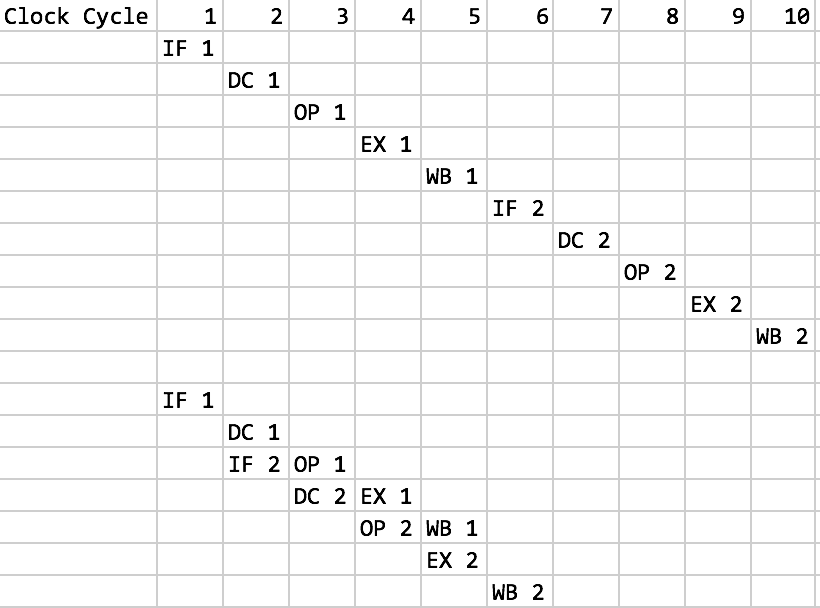
\includegraphics[width=0.4\textwidth]{images/pipelining}
\end{center}

In the above image, two instructions are shown. The top part shows no pipelining; the bottom shows what happens when pipelining is used. Each part of the instruction must be done sequentially -- the instruction cannot be decoded until it is fetched -- but at least the next instruction can be done. So it allows each of these to appear as if it is 1 clock cycle. If all goes well, then you complete one instruction per clock cycle. 

But there are pipeline hazards: sometimes you need the result of a previous step before you can go on. These prevent us from reaching the theoretical maximum of one instruction completed per clock cycle. Needing a previous result is not the only kind of hazard, though; we may have conflicts over certain CPU resources (how many floating point units are there, after all...?) or fetch may be unable to identify the next instruction because of a branch. In the worst case, if we have mispredicted a branch, we have to flush the pipeline: throw away the instructions fetched, decoded, operands prepared, et cetera, because we guessed wrong and started doing the wrong actions. In that case, some extra work was done that was not necessary... 

The next idea relates to getting items from memory. If we do a load from memory, and we are lucky, it is found in the fastest cache and is available in perhaps 2-3 clock cycles. If we must go to memory, it may be 200-300 cycles. If it is in level 2 or level 3 cache it will be somewhere in between. The key idea, though, is if we are trying to put something in register \texttt{R7}, it will take time until that value is actually present in that register. The simplest approach is to just wait around until that value has arrived, and then go on to the next instruction. That works, but we can do better.

That better idea is: continue executing until \texttt{R7} is used somewhere. This allows us to get some useful work done in the meantime. Hardware keeps track of the fact that the register is not quite ready yet, but the work can get done in what is called the ``miss shadow''. It's possible to have more than one load in flight at a time. Two or more can be done in various CPU architectures, but it is of course hardware dependant. 

Branch prediction has come up already, but if we have a load followed by a compare used as a branch, we can then, well, guess. If we are wrong, there is the need to cleanup. But the good news is that branch prediction is usually right most of the time, perhaps 95\% or more (we'll definitely return to this later).

Another nice thing that the hardware can do for us is ``dual issue'' instructions. If we have two consecutive instructions that both take the same amount of time, use unrelated registers, and don't consume two of the same resource, we can start both instructions at once. If the instructions are \texttt{ADD R1, 16} and \texttt{CMP R2, 0} they do different things with different registers so there is no reason these cannot be done in parallel (if there are enough fetch/decode/etc units). In an embedded system, you may be interested in ensuring that this happens during a computationally intensive loop, such as encoding/decoding of media. If programmed correctly, you can be sure you get dual issue on every cycle.

Then a group of things that somewhat go together: register renaming, branch prediction, speculation, and Out-of-Order (O-O-O) Execution. These all work synergistically: each adds to the benefits the other brings. Register renaming works on a fairly simple principle: an assembly instruction says to read from register \texttt{R4}, but behind the scenes inside the processor, it is mapped to a physical register (let's say \texttt{RA} for the purpose of the example). Consider the following assembly instructions:

\begin{verbatim}
MOV R2, R7 + 32
ADD R1, R2
MOV R2, R9 + 64
ADD R3, R2
\end{verbatim}

Under normal circumstances, we cannot do instruction 3 until instruction 2 has been completed because we need the value of \texttt{R2} that was put in there (taken from memory somewhere) to be added to \texttt{R1}. Except, with register renaming, behind the scenes the first two instructions may replace \texttt{R2} with \texttt{RX} and the second pair of instructions have \texttt{R2} replaced with \texttt{RY} and these things can take place in parallel, or without a stall, at the very least.

This has a certain synergy with branch prediction. If we predict a branch, we can do speculative changes into one set of registers while we keep the ``old'' register values around too. When we figure out whether the branch prediction is correct, we can then get rid of the ones we don't need: the originals if predicted correctly, and the new values otherwise. So we get better recovery if there is a misprediction. Actually, I bet students wish they could do this: write down both answers to a question and let the TA pick the correct one at the end...

Most importantly, it allows us to get past a cache miss and keep going; the goal here is to run until we can start the next cache miss, because the sooner that starts the sooner it's over, and the faster the program executes, ultimately. A quick example from the presentation demonstrates this, in x86 assembly~\cite{modern-hardware}:

\begin{verbatim}
ld rax, rbx+16   ; assume cache miss
add rbx, 16      ; carry on anyway, ADD doesn't need rax value from LD
                 ; register renaming => LD (write)/ADD (read) don't interfere
cmp rax, 0       ; needs rax value, queue till available
jeq null_chk     ; oops! need cmp result
                 ; speculate: assume branch not taken
st rbx-16, rcx   ; speculatively store to store buf (not L1)
ld rcx, rdx      ; unrelated cache miss: 2 misses now active, 1 speculative
ld rax, rax+8    ; now must wait for result of first LD
\end{verbatim}

%Let's assume \texttt{rax} (register A) is not available and the first instruction is a cache miss and it will take 300 cycles to get it. So we carry on. Then the instruction next is unrelated so we can go on. It doesn't matter that \texttt{rbx} is read in the first two instructions, because we can do register renaming so that internally it's reading from register 4 and writing to register 12. The compare cannot proceed because the first load's value is not available, but it will be queued up to be done later. Then we have a branch, but we don't know what the flags are, because we can't compare, because the load isn't done. The branch predictor will say in this example that we will not take the branch and go on to the store instruction (\texttt{st}). The store is speculative because the branch may have been taken (so it goes in a store buffer temporarily and not to L1 cache, until we are sure it's okay to let it go to memory). We have now made it to the second last line and we have another unrelated cache miss, and we have two cache misses running in parallel (the second of which is speculative). Finally, the last instruction has to wait for the first instruction to fill the register \texttt{rax} and we can no longer speculate.

To summarize: there are seven operations we were trying to do here with two cache misses. The cache misses complete in cycles 300 and 304 (maybe 302 if we have dual issue), so in total we complete 7 operations in about 305 cycles. All the trickery and cleverness got us to that second miss which means we complete in 305. If we did not manage that, it would take about 600 cycles to complete it all. So we did double performance, even though in this example our overall performance was terrible.
 
For years Intel was trying to push its Itanium processors (which were so unsuccessful they got the nickname ``Itanic''. Ouch). The goal of these was to find static (compile-time) parallelism: if a machine has infinite registers, can speculate infinitely, etc, the program gets sped up. Run all possibilities in parallel and at the end figure out which is right (wasn't this a Nicolas Cage movie?). Unfortunately it didn't work out very well because this requires the right kind of program and an super smart compiler. Oh yes, and infinite registers requires infinite space as well as infinite money. So instead the quest has turned to how we can get better performance out of x86\ldots

The x86 approach tries to maximize dynamic (run-time) parallelism. This has been done incrementally, with more pipelining, re-order buffers, adding more functional units, and so on. But the walls are still there: cache miss rates and branch mispredicts continue to dominate performance, even though the rates are very low, because a miss costs so much. 

How are we doing so far? Well, here's a short video that goes over where we were in the beginning of 2017: \url{https://www.youtube.com/watch?v=4A0Iks4ENIs} with the launch of Intel's latest (at the time) processor. But since then, AMD launched Ryzen -- Never turn your back on Threadripper! -- and it's forced Intel to compete again... 

According to~\cite{modern-hardware} something like 90-99\% of the transistors on a modern x86 chip are spent in cache. In spite of the extreme complexity of the decode logic that allows multiple parallel decodes of all the weird and wacky instructions of the x86, pushing cache to the biggest size it can be is so important because it prevents the performance hit of going to memory.

The image below (from Sun World Wide Analyst Conference in 2003) is obviously a bit dated but this is very instructive as to the trend:
\begin{center}
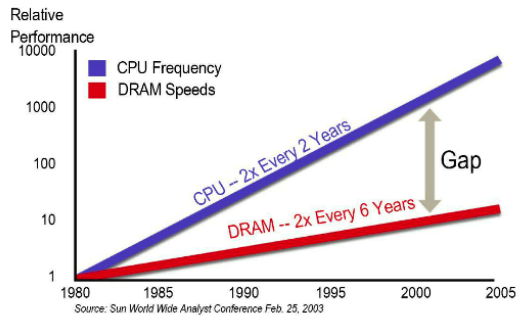
\includegraphics[width=0.6\textwidth]{images/ram-vs-cpu.png}
\end{center}

DRAM is, however, not the only kind of memory. There is SRAM (Static RAM) which is fast but expensive, the kind of stuff that goes on the CPU die, and it is six transistors per bit. Compare against DRAM which is much cheaper, but slow: one transistor and one capacitor per bit. Improvements in DRAM have not really improved latency but have improved bandwidth; DDR (Dual Data Rate... not Dance Dance Revolution) means there are two transfers per cycle, but it still takes significant time to get any data out. And DRAM needs occasional refreshes (capacitors...) so sometimes we have to wait for that.

In the Operating Systems course you probably learned that disk is the slowest thing and the limiting factor. That's true, as Obi-Wan Kenobi would say, from a certain point of view. Now that we live in the world of Solid State Drives (SSDs), ``disk'' reads are about as fast as memory reads and memory reads are the rate-limiting step in the system. Nonvolatile memory looks to be even faster. More is the new more, orange is the new black, and memory is the new disk.

To get memory access speed up there are things we can do, like relax coherency constraints, more synchronization through locks... all of which we will come back to in some upcoming lectures. 

If we want to get better performance, we need to figure out where time is going. For that we will have the subject of profiling, which comes up in some later lectures. If we can track down where our cache misses are occurring, maybe, just maybe, we can do something about it. 

\section*{A Deeper Look at Cache Misses}

As discussed, the CPU generates a memory address for a read or write operation. The address will be mapped to a page. Ideally, the page is found in the cache, because that would be faster. If the requested page is, in fact,  in the cache, we call that a cache \textit{hit}. If the page is not found in the cache, it is considered a cache \textit{miss}. In case of a miss, we must load the page from memory, a comparatively slow operation. The percentage of the time that a page is found in the cache is called the \textit{hit ratio}, because it is how often we have a cache hit. We can calculate the effective access time if we have a good estimate of the hit ratio (which is not overly difficult to obtain) and some measurements of how long it takes to load data from the cache and how long from memory. The effective access time is therefore computed as:

\begin{center}
Effective Access Time = $h \times t_{c} + (1-h) \times t_{m}$
\end{center}

Where $h$ is the hit ratio, $t_{c}$ is the time required to load a page from cache, and $t_{m}$ is the time to load a page from memory. Of course, we would like the hit ratio to be as high as possible. 

Caches have limited size, because faster caches are more expensive. With infinite money we might put everything in registers, but that is rather unrealistic. Caches for memory are very often multileveled; Intel 64-bit CPUs tend to have L1, L2, and L3 caches. L1 is the smallest and L3 is the largest. Obviously, the effective access time formula needs to be updated and expanded when we have multiple levels of cache with different access times and hit rates. See the diagram below:

\begin{center}
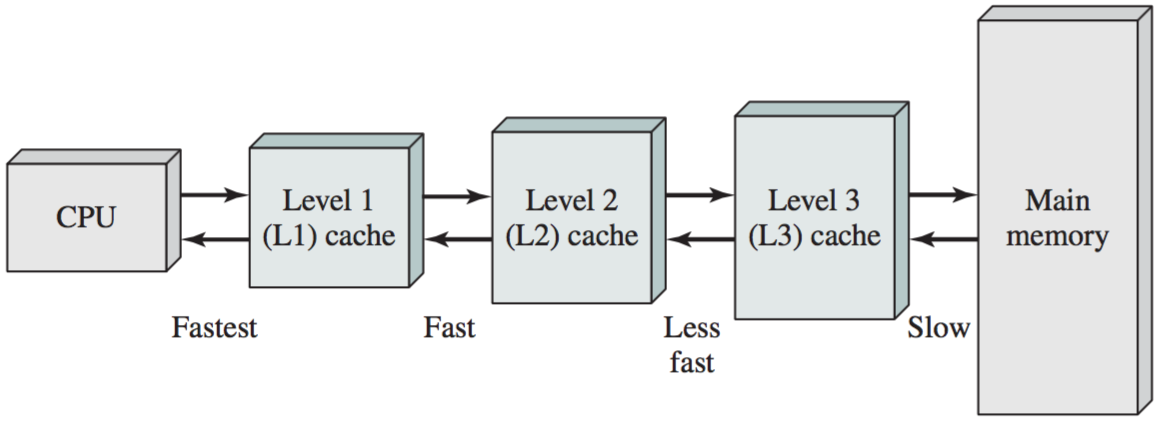
\includegraphics[width=0.6\textwidth]{images/caches.png}\\
Three levels of cache between the CPU and main memory~\cite{osi}.
\end{center}

If we have a miss in the L1 cache, the L2 cache is checked. If the L2 cache contains the desired page, it will be copied to the L1 cache and sent to the CPU. If it is not in L2, then L3 is checked. If it is not there either, it is in main memory and will be retrieved from there and copied to the in-between levels on its way to the CPU. 

Cliff Click said that 5\% miss rates dominate performance. Let's look at why.
I looked up a characterization of the SPEC CPU2000 and CPU2006 
benchmarks~\cite{cpu2006}.

Here are the reported cache miss rates\footnote{\permil~is ``permil'', or per-1000.} for SPEC CPU2006.

\begin{center}
\begin{tabular}{ll}
L1D & 40\permil \\
L2 & 4 \permil
\end{tabular}
\end{center}

Let's assume that the L1D cache miss penalty is 5 cycles and the L2 miss penalty is
300 cycles, as in the video. Then, for every instruction, you would expect a running
time of, on average:
\[ 1 + 0.04 \times 5 + 0.004 \times 300 = 2.4. \]
Misses are expensive!


If we replace the terms $t_{c}$ and $t_{m}$ with $t_{m}$ and $t_{d}$ (time to retrieve it from disk) respectively, and redefine $h$ as $p$, the chance that a page is in memory, we can get an idea of the effective access time in virtual memory: 

\begin{center}
	Effective Access Time = $ p \times t_{m} + (1 - p) \times t_{d}$
\end{center}

And just while we're at it, we can combine the caching and disk read formulae to get the true effective access time for a system where there is only one level of cache:

\begin{center}
	Effective Access Time = $ h \times t_{c} + (1 - h) ( p \times t_{m} + (1 - p) \times t_{d})$
\end{center}

This is good, but what is $t_{d}$? This is a measurable quantity so it is possible, of course, to just measure it\footnote{One of my favourite engineering sayings is ``Don't guess; measure.'' You may be sick of hearing me say that one by now.}.

The slow step in all of this, is obviously, the amount of time it takes to load the page from disk. According to~\cite{osc}, restarting the process and managing memory and such take something like 1 to 100~$\mu$s. A typical hard drive in their example has a latency of 3~ms, seek time (moving the read head of the disk to the location of the page) is around 5~ms, and a transfer time of 0.05~ms. So the latency plus seek time is the limiting component, and it's several orders of magnitude larger than any of the other costs in the system. And this is for servicing a request; don't forget that several requests may be queued, making the time even longer.

Thus the disk read term $t_{d}$ dominates the effective access time equation. If memory access takes 200~ns and a disk read 8~ms, we can roughly estimate the access time in nanoseconds as $(1-p) \times 8~000~000$. 

If the page fault rate is high, performance is awful. If performance of the computer is to be reasonable, the page fault rate has to be very, very low.

Summary: misses are not just expensive, they hurt performance more than anything else.










\chapter*{3 --- CPU Hardware, Branch Prediction}

\addcontentsline{toc}{chapter}{3 --- CPU Hardware, Branch Prediction}

\section*{Multicore Processors}
As I've alluded to earlier, multicore processors came about because
clock speeds just aren't going up anymore. We'll discuss technical
details today. Each processor \emph{core} executes instructions; a processor with more than one core can therefore simultaneously execute multiple
(unrelated) instructions. 

\paragraph{Chips and cores.} Multiprocessor (usually SMP, or symmetric
multiprocessor) systems have been around for a while. Such systems
contain more than one CPU. We can count the number of CPUs by
physically looking at the board; each CPU is a discrete physical thing.

Cores, on the other hand, are harder to count. In fact, they look just
like distinct CPUs to the operating system:

{\scriptsize \begin{verbatim}
plam@plym:~/courses/p4p/lectures$ cat /proc/cpuinfo
processor	: 0
vendor_id	: GenuineIntel
cpu family	: 6
model		: 23
model name	: Pentium(R) Dual-Core  CPU      E6300  @ 2.80GHz
...
processor	: 1
vendor_id	: GenuineIntel
cpu family	: 6
model		: 23
model name	: Pentium(R) Dual-Core  CPU      E6300  @ 2.80GHz
\end{verbatim}
}
\vspace*{-1em}
%$ 
If you actually opened my computer, though, you'd only find one chip.
The chip is pretending to have two \emph{virtual CPUs}, and the
operating system can schedule work on each of these CPUs. In general,
you can't look at the chip and figure out how many cores it contains.

\vspace*{-1em}
\paragraph{Hardware Designs for Multicores.}
In terms of the hardware design, cores might share a cache, as in this picture:

\vspace*{-1em}
\begin{center}
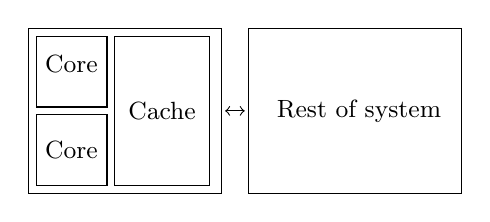
\begin{tikzpicture}
\draw (-0.5, -0.5) rectangle ++(0.9, 0.9);
\draw (-0.05, 0.05) node {\small Core};

\draw (-0.5, -1.5) rectangle ++(0.9, 0.9);
\draw (-0.05, -1.05) node {\small Core};

\draw (0.5, -1.5) rectangle ++(1.2, 1.9);
\draw (1.1, -.55) node {\small Cache};

\draw (-0.6, -1.6) rectangle ++(2.45, 2.1);

\draw (2.2, -1.6) rectangle ++(2.7, 2.1);
\draw (3.6, -0.55) node {\small Rest of system};

\draw[<->] (1.9, -0.55) -- (2.15, -0.55);
\end{tikzpicture}
\end{center}
\vspace*{-1em}
\hfill (credit: \emph{Multicore Application Programming}, p. 5)

This above Symmetric Multithreading (SMP) design is especially good for the 1:1 threading model. In
this case, the design of the cores don't need to change much, but they
still need to communicate with each other and the rest of the system.

Or, we can have a design that works well for the N:1 model:
\begin{center}
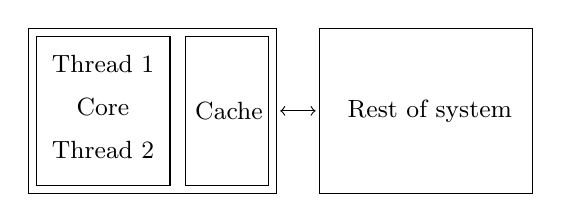
\begin{tikzpicture}
\draw (-1.4, -1.5) rectangle ++(1.7, 1.9);
\draw (-0.55, 0.05) node {\small Thread 1};
\draw (-0.55, -1.05) node {\small Thread 2};
\draw (-0.55, -0.5) node {\small Core};

\draw (0.5, -1.5) rectangle ++(1.05, 1.9);
\draw (1.05, -.55) node {\small Cache};

\draw (-1.5, -1.6) rectangle ++(3.15, 2.1);

\draw (2.2, -1.6) rectangle ++(2.7, 2.1);
\draw (3.6, -0.55) node {\small Rest of system};

\draw[<->] (1.7, -0.55) -- (2.15, -0.55);
\end{tikzpicture}
\end{center}

One would expect that executing two threads on one core might
mean that each thread would run more slowly. It depends on the instruction
mix. If the threads are trying to access the same resource, then each
thread would run more slowly. If they're doing different things, there's 
potential for speedup.

Finally, it's possible to both use multiple cores and put multiple threads
onto one core, as in the M:N model:

\begin{center}
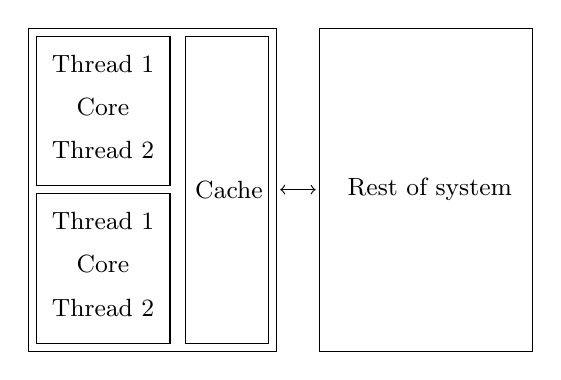
\begin{tikzpicture}

 \draw (-1.4, -1.5) rectangle +(1.7, 1.9);
 \draw (-1.4, -3.5) rectangle +(1.7, 1.9);

\foreach \y in {-2, 0}
{
 \draw (-0.55, 0.05) + (0, \y) node {\small Thread 1};
 \draw (-0.55, -1.05) + (0, \y) node {\small Thread 2};
 \draw (-0.55, -0.5) + (0, \y) node {\small Core};
}

\draw (0.5, -3.5) rectangle ++(1.05, 3.9);
\draw (1.05, -1.55) node {\small Cache};

\draw (-1.5, -3.6) rectangle ++(3.15, 4.1);

\draw (2.2, -3.6) rectangle ++(2.7, 4.1);
\draw (3.6, -1.55) node {\small Rest of system};

\draw[<->] (1.7, -1.55) -- (2.15, -1.55);
\end{tikzpicture}
\end{center}
Here we have four hardware threads; pairs of threads share hardware
resources. One example of a processor which supports chip multi-threading
(CMT) is the UltraSPARC T2, which has 8 cores, each of which supports 8 
threads. All of the cores share a common level 2 cache.

\paragraph{Non-SMP systems.} The designs we've seen above have been
more or less SMP designs; all of the cores are mostly alike.
A very non-SMP system is the Cell, which contains a PowerPC main core
(the PPE) and 7 Synergistic Processing Elements (SPEs), which are
small vector computers.


\paragraph{Non-Uniform Memory Access.}
In SMP systems, all CPUs have approximately the same access time for resources
(subject to cache misses). There are also NUMA, or Non-Uniform Memory Access,
systems out there. In that case, CPUs can access different resources at different
speeds. (Resources goes beyond just memory).

In this case, the operating system should schedule tasks on CPUs which
can access resources faster.  Since memory is commonly the bottleneck,
each CPU has its own memory bank.

\paragraph{Using CMT effectively.} Typically, a CPU will expose its
hardware threads using virtual CPUs.
In current hardware designs, each of the hardware threads has the same
performance. 

However, performance varies depending on context. In the above
example, two threads running on the same core will most probably run
more slowly than two threads running on separate cores, since they'd
contend for the same core's resources. Task switches between cores (or
CPUs!) are also slow, as they may involve reloading caches.

Solaris ``processor sets''
enable the operating system to assign processes to specific virtual CPUs,
while Linux's ``affinity'' keeps a process running on the same virtual CPU.
Both of these features reduce the number of task switches, and processor
sets can help reduce resource contention, along with Solaris's locality
groups.\footnote{Gove suggests that locality groups help reduce contention
for core resources, but they seem to help more with memory.}



\section*{Branch Prediction and Misprediction}

The compiler (and the CPU) take a look at code that results in branch instructions  such as loops, conditionals, or the dreaded \texttt{goto}\footnote{Which I still maintain is a swear word in C.}, and it will take an assessment of what it thinks is likely to happen. By default I think it's assumed that backward branches are taken and forward branches are not taken (but that may be wrong).  Well, how did we get here anyway?

In the beginning the CPUs and compilers didn't really think about this sort of thing, they would just come across instructions one at a time and do them and that was that. If one of them required a branch, it was no real issue. Then we had pipelining: the CPU would fetch the next instruction while decoding the previous one, and while executing the instruction before. That means if evaluation of an instruction results in a branch, we might go somewhere else and therefore throw away the contents of the pipeline. Thus we'd have wasted some time and effort. If the pipeline is short, this is not very expensive. But pipelines keep getting longer\ldots

So then we got to the subject of branch prediction. The compiler and CPU look at instructions on their way to be executed and analyze whether it thinks it's likely the branch is taken. This can be based on several things, including the recent execution history. If we guess correctly, this is great, because it minimizes the cost of the branch. If we guess wrong, we have to flush the pipeline and take the performance penalty.

The compiler and CPU's branch prediction routines are pretty smart. Trying to outsmart them isn't necessarily a good idea. But we can give the compiler (\texttt{gcc} at least) some hints about what we think is likely to happen. Our tool for this is the \texttt{\_\_builtin\_expect()} function, which takes two arguments, the value to be tested and the expected result.

In the linux \texttt{compiler.h} header there are two neat little shortcuts defined:

\begin{lstlisting}[language=C]
# define likely(x)      __builtin_expect(!!(x), 1)
# define unlikely(x)    __builtin_expect(!!(x), 0)
\end{lstlisting}

These are nice ways of saying that we expect \texttt{x} to be true (likely) or false (unlikely). These hints tell the compiler some information about how it should predict. It will then arrange the instructions in such a way that, if the prediction is right, the instructions in the pipeline will be executed. But if we're wrong, then the instructions will have to be flushed.

Compile with at least optimization level 2 (\texttt{-O2}) for the compiler to take these hints. Otherwise they won't do anything. 

It takes a bit of trickery to force branch mispredicts. {\tt gcc} extensions allow hinting, but usually {\tt gcc} or the processor is smart enough to ignore bad hints. This code from~\cite{mispredict} worked in 2013, though:


\begin{lstlisting}[language=C]
        #include <stdlib.h>
        #include <stdio.h>

        static __attribute__ ((noinline)) int f(int a) { return a; }

        #define BSIZE 1000000
        int main(int argc, char* argv[]) 
        {
          int *p = calloc(BSIZE, sizeof(int));
          int j, k, m1 = 0, m2 = 0;
          for (j = 0; j < 1000; j++) {
            for (k = 0; k < BSIZE; k++) {
              if (__builtin_expect(p[k], EXPECT_RESULT)) {
                m1 = f(++m1);
              } else {
                m2 = f(++m2);
              }
            }
          }
          printf("%d, %d\n", m1, m2);
        }
\end{lstlisting}

Running it yielded:
\begin{lstlisting}[language=C]
plam@plym:~/459$ gcc -O2 likely-simplified.c -DEXPECT_RESULT=0 -o likely-simplified
plam@plym:~/459$ time ./likely-simplified
0, 1000000000

real	0m2.521s
user	0m2.496s
sys	0m0.000s
plam@plym:~/459$ gcc -O2 likely-simplified.c -DEXPECT_RESULT=1 -o likely-simplified
plam@plym:~/459$ time ./likely-simplified
0, 1000000000

real	0m3.938s
user	0m3.868ss
sys	0m0.000s
\end{lstlisting}
Some versions of {\tt gcc} and {\tt clang} seem to have gotten smart enough to reject bogus hints since then. In 2018, gcc 7.2.0 shows the same time on Linux 4.14.12 (post-mitigation) running on a Pentium G645, while clang 6.0.0 shows a difference of 2.46s vs 2.81s.

In the original source~\cite{mispredict} the author reports the following results: scanning a one million element array, with all elements initially zero, the results are:
\vspace*{-1em}
\begin{itemize}[noitemsep]
	\item No use of hints: \texttt{0:02.68 real,  2.67 user, 0.00 sys}
	\item Good prediction: \texttt{0:02.28 real,  2.28 user, 0.00 sys}
	\item Bad prediction: \texttt{0:04.19 real,  4.18 user, 0.00 sys}
\end{itemize}

\paragraph{Using the hints.} From these results we can see pretty clearly that if we're wrong, the penalty can be pretty large (assuming the compiler does not look at your hint and think ``stupid human, I know better''). Under a lot of circumstances then, it's probably best just to leave it alone, unless we're really, really, really sure. 

How sure do we have to be? The answer depends dramatically on the code, the CPU you're using, the compiler, and all those little details. But~\cite{mispredict} to the rescue here again, because there are some tests here. To cut to the chase, when about one in ten thousand values in the array is nonzero, then it's roughly the ``break-even'' point for the setup as described.

Conclusion: it's hard to outsmart the compiler. Maybe it's better not to try.

\subsection*{How does branch prediction work, anyway?}
We can write software. The hardware will make it fast. If we understand the hardware, we can understand when it has trouble making our software fast.

You've seen how branch prediction works in ECE 222. However, we'll talk about it today in the context of performance. Notes based on a transcript of a talk by Dan Luu~\cite{branchprediction}.

I want you to pick up two points from this discussion:
\vspace*{-1em}
\begin{itemize}[noitemsep]
\item how branch predictors work---this helps you understand some of the apparent randomness in your
execution times, and possibly helps you make your code more predictable; and,
\item applying a (straightforward) expected value computation to predict performance.
\end{itemize}

Let's consider the following assembly code:

\hspace*{2em} \begin{minipage}{.4\textwidth} \begin{lstlisting}
branch_if_not_equal x, 0, else_label
// Do stuff
goto end_label
else_label:
// Do things
end_label:
// whatever happens later
\end{lstlisting}
\end{minipage}

The {\tt branch} instruction may be followed by either ``stuff'' or ``things''.
The pipeline needs to know what the next instruction is, for instance to fetch it.
But it can't know the next instruction until it almost finishes executing the branch.
Let's look at some pictures, assuming a 2-stage pipeline.

With no prediction, we need to serialize:

\begin{center}
\begin{tabular}{c|c|c|c}
bne.1 & bne.2 \\ \hline
& & things.1 & things.2
\end{tabular}
\end{center}

\begin{minipage}{.49\textwidth}
Let's predict that ``things'' gets taken.
If our prediction is correct, we save time.

\begin{center}
\begin{tabular}{c|c|c}
bne.1 & bne.2 \\ \hline
& things.1 & things.2 \\
\\
\end{tabular}
\end{center}
\end{minipage} \hspace*{.02\textwidth} \begin{minipage}{.49\textwidth}
But we might be wrong and need to throw out the bad prediction.

\begin{center}
\begin{tabular}{c|c|c|c}
bne.1 & bne.2 \\ \cline{1-2}
& \sout{things.1} \\ \hline
& & stuff.1 & stuff.2
\end{tabular}
\end{center}
\end{minipage}

\paragraph{Cartoon model.} We need to quantify the performance.
For the purpose of this lecture, let's pretend that our pipelined
CPU executes, on average, one instruction per clock;
mispredicted branches cost 20 cycles, while correctly-predicted
branches cost 1 cycle. We'll also assume that the instruction
mix contains 80\% non-branches and 20\% branches. So we can predict
average cycles per instruction.

With no prediction (or always-wrong prediction):
\[
\mathrm{non\_branch\_\%} \times 1 \mathrm{~cycle} + \mathrm{branch\_\%} \times 20 \mathrm{~cycles} = 4.8 \mathrm{~cycles}.
\]
With perfect branch prediction:
\[
\mathrm{non\_branch\_\%} \times 1 \mathrm{~cycle} + \mathrm{branch\_\%} \times 1 \mathrm{~cycle} = 1 \mathrm{~cycle}.
\]
So we can make our code run 4.8$\times$ faster with branch prediction!

\paragraph{Predict taken.} What's the simplest possible thing? We can
predict that a branch is always taken. (Loop branches, for instance,
account for many of the branches in an execution, and are often taken.)
If we got 70\% accuracy, then our cycles per instruction would be:
\[
(0.8 + 0.7 \times 0.2) \times 1 \mathrm{~cycle} + (0.3 \times 0.2) \times 20 \mathrm{~cycles} = 2.14 \mathrm{~cycles}.
\]
The simplest possible thing already greatly improves the CPU's average throughput.

\paragraph{Backwards taken, forwards not taken (BTFNT).}
Let's leverage that observation about loop branches to do better.
Loop branches are, by definition, backwards (go back to previous
code). So we can design a branch predictor which predicts ``taken''
for backwards and ``not taken'' for forwards. The compiler can then
use this information to encode what it thinks about forwards branches
(that is, making the not-taken branch the one it thinks is more likely).
Let's say that this might get us to 80\% accuracy. \[
(0.8 + 0.8 \times 0.2) \times 1 \mathrm{~cycle} + (0.2 \times 0.2) \times 20 \mathrm{~cycles} = 1.76 \mathrm{~cycles}.
\]
The PPC 601 (1993) and 603 used this scheme.

\paragraph{Going dynamic: using history for branch prediction.}
So far, we will always make the same prediction at each branch---known as a
\emph{static} scheme. But we can do better by using what recently happened to
improve our predictions. This is particularly important when program execution
contains distinct phases, with distinct behaviours.
We therefore move to \emph{dynamic} schemes.

Once again, let's start with the simplest possible thing. For every branch,
we record whether it was taken or not last time it executed (a 1-bit scheme).
Of course, we can't store all branches. So let's use the low 6 bits of the address
to identify branches. Doing so raises the prospect of \emph{aliasing}:
different branches (with different behaviour) map to the same spot in the table.

We might get 85\% accuracy with such a scheme.
\[
(0.8 + 0.85 \times 0.2) \times 1 \mathrm{~cycle} + (0.15 \times 0.2) \times 20 \mathrm{~cycles} = 1.57 \mathrm{~cycles}.
\]

At the cost of more hardware, we get noticeable performance improvements. The DEC EV4 (1992) and
MIPS R8000 (1994) used this one-bit scheme.

\paragraph{Two-bit schemes.}
What if a branch is almost always taken but occasionally not taken (e.g. TTTTTTNTTTT)?
We get penalized twice
for that misprediction: once when we mispredict the not taken, and once when we mispredict the
next taken. So, let's store whether a branch is ``usually'' taken, using a so-called
2-bit saturating counter.

Every time we see a taken branch, we increment the counter for that
branch; every time we see a not-taken branch, we decrement. Saturating
means that we don't overflow or underflow. We instead stay at 11 or
00, respectively.

If the counter is 00 or 01, we predict ``not taken''; if it is 10 or
11, we predict ``taken''.

With a two-bit counter, we can have fewer entries at the same size, but they'll do better.
It would be reasonable to expect 90\% accuracy.
\[
(0.8 + 0.9 \times 0.2) \times 1 \mathrm{~cycle} + (0.1 \times 0.2) \times 20 \mathrm{~cycles} = 1.38 \mathrm{~cycles}.
\]

This was used in a number of chips, from the LLNL S-1 (1977) through the Intel Pentium (1993).

\paragraph{Two-level adaptive, global.}
We're still not taking patterns into account. Consider the following {\tt for} loop.
\begin{lstlisting}[language=C]
for (int i = 0; i < 3; ++i) {
  // code
}
\end{lstlisting}
The last three executions of the branch determine the next direction:
\begin{verbatim}
 TTT => N
 TTN => T
 TNT => T
 NTT => T
\end{verbatim}
Let's store what happened the last few times we were at a particular address---the
\emph{branch history}. From a branch address and history, we derive an index, which
points to a table of 2-bit saturating counters. What's changed from the two-bit scheme
is that the history helps determine the index and hence the prediction.

After we take a branch, we add its direction to the history, so that the next lookup
maps to a different table entry.

This scheme might give something like 93\% accuracy.
\[
(0.8 + 0.93 \times 0.2) \times 1 \mathrm{~cycle} + (0.07 \times 0.2) \times 20 \mathrm{~cycles} = 1.27 \mathrm{~cycles}.
\]

The Pentium MMX (1996) used a 4-bit global branch history.

\paragraph{Two-level adaptive, local.}
The change here is that the CPU keeps a separate history for each branch.
So the branch address determines which branch history gets used.
We concatenate the address and history to get the index, which then points to a
2-bit counter again. We are starting to encounter diminishing returns, but we might
get 94\% accuracy:
\[
(0.8 + 0.94 \times 0.2) \times 1 \mathrm{~cycle} + (0.06 \times 0.2) \times 20 \mathrm{~cycles} = 1.23 \mathrm{~cycles}.
\]

The Pentium Pro (1996), Pentium II (1997) and Pentium III (1999) use this.

\paragraph{gshare.}
Instead of concatenating the address and history, we can xor them. This allows
us to use more bits for both the history and address. This keeps the accuracy the same,
but simplifies the design.

\paragraph{Other predictors.} We can build (and people have built) more sophisticated predictors.
These predictors could, for instance, better handle aliasing, where
different branches/histories map to the same index in the table. But we'll stop here.

\paragraph{Summary of branch prediction.} We can summarize as follows.
Branch prediction enables pipelining and hence increased performance.
We can create a model to estimate just how critical branch prediction
is for modern processors. Fortunately, most branches are predictable
now. Aliasing (multiple branches mapping to the same entry in a
prediction table) can be a problem, but processors are pretty good at
dealing with that too.

\section*{Side-channel attacks}
There's been a lot happening lately in terms of exploiting the hardware of CPU architectures to get access to privileged data, and unfortunately these things have performance implications!

\subsection*{Cache Attacks}
In early 2018, the Spectre~\cite{Kocher2018spectre} and Meltdown~\cite{Lipp2018meltdown} attacks were disclosed. These attacks leverage performance features of modern CPUs to break process isolation guarantees---in principle, a process shouldn't be able to read memory that belongs to the kernel or to other processes.

The concept of cache side-channel attacks has been known for a while. If an attacker can get some memory loaded into the cache, then it can extract that memory using a cache side-channel attack.

Spectre and Meltdown can cause privileged memory to be loaded into the cache, and then extracted using a cache side-channel attack. We'll talk about Spectre (variant 2), since it attacks branch prediction in particular. My explanation follows~\cite{masters18:_what_meltd_spect} by Jon Masters of RedHat. However, you should now have enough background to follow the Google Project Zero description at~\cite{horn18:_readin}.

We know that at a branch, the CPU will start speculatively executing code at the inferred target of the branch. To exploit this vulnerability, the attack code convinces the CPU to speculatively execute code of its choice. The speculatively-executed attack code reads secret data (e.g. from the hypervisor kernel) and puts it in the cache. Once the data is in the cache, the attack proceeds by extracting the data from the cache.

Unfortunately, the only mitigation thus far involved additional security measures (in hardware and software) that unfortunately result in lower performance in program execution.

\subsection*{Hyperthreading attacks}
Multiprocessor (multicore) processors have some hardware that tries to keep the data consistent between different pipelines and caches (as we saw in the video). More processors, more threads means more work is necessary to keep these things in order. We will discuss cache coherence soon, but about hyperthreading... it turns out this is vulnerable too.

Remember that in hyperthreading, two threads are sharing the same execution core. That means they have hardware in common. Because of this, a thread can figure out what the other thread is doing by noticing its cache accesses and by timing how long it takes to complete operations. This is like sitting next to someone who's taking a multiple choice exam and noticing what answers they are choosing by how long it takes them to move their pencil down the page to fill in the correct circle. Yes, you have to be running on the same CPU as the victim, but still... Yikes! 

Researchers discovered and published a paper~\cite{portsmash} detailing the attack and showing a practical implementation of it. In the practical example, a 384-bit secret key is (over time) completely stolen by another process. It seems likely that this will lead in the long term to slowdowns of existing hardware as Operating System patches will need to prevent threads from different processes from using the same core... And possibly the only long term solution is to not use hyperthreading at all... the performance implications of which are both obvious and significant.









\chapter*{4 --- Cache Coherency}

\addcontentsline{toc}{chapter}{4 --- Cache Coherency}

\section*{Cache Coherency}

\begin{center}
    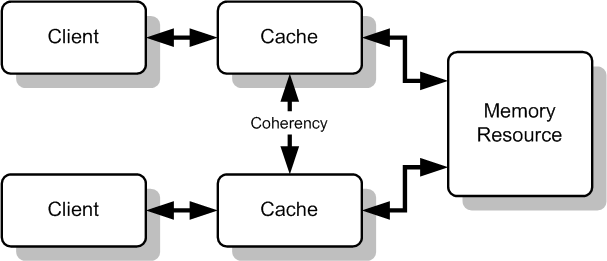
\includegraphics[width=0.5\textwidth]{images/coherency}

\hfill ---Wikipedia
\end{center}

Today we'll look at what support the architecture provides for memory ordering, in
particular in the form of cache coherence. Since this isn't an
architecture course, we'll look at this material more from the point
of view of a user, not an implementer.

The problem is, of course, that each CPU likely its own cache. If it does then these data may be out of sync -- the value that CPU 1 has for a particular piece of data might be different from the value that CPU 4 has. The simplest method, and a horrible solution, would be the ability to declare some read/write variables as being non-cacheable (is that a word? Uncacheable?...). The compiler and OS and such will require the data to be read from main memory, always. This will obviously result in lower cache hit ratios, increased bus traffic, and terrible, terrible performance. Let's avoid that. What we want instead is \textit{coherency}.

Cache coherency means that:
  \begin{itemize}
    \item the values in all caches are consistent; and
    \item to some extent, the system behaves as if all CPUs are using shared memory.
  \end{itemize}
  
In modern CPUs with three or four levels of cache, we frequently find that the level 3 cache isn't much faster than going to main memory. But this level is where the cache coherency communication can take place. This can be by making the cache shared between the different CPUs. And the L4 cache is frequently used for sharing data with the integrated graphics hardware on CPUs that have this feature. But for the most part we will imagine that caches are not shared, and we have to figure out how to get coherency between them. This is the case with a L1/L2 cache in a typical modern CPU as they are unique to the given core (i.e., not shared).
  
\paragraph{Cache Coherence Example.} We will use this example to illustrate
different cache coherence algorithms and how they handle the same situation.

Initially in main memory: {\tt x = 7}.

  \begin{enumerate}
    \item {\tt CPU1} reads x, puts the value in its cache.
    \item {\tt CPU3} reads x, puts the value in its cache.
    \item {\tt CPU3} modifies {\tt x := 42}
    \item {\tt CPU1} reads x \ldots ~from its cache?
    \item {\tt CPU2} reads x. Which value does it get?
  \end{enumerate}

Unless we do something, {\tt CPU1} is going to read invalid data.
  
Outside of a computing context, imagine you and several co-workers have some shared information, such as a meeting (in a specific room) in a shared online calendar (the one for the room). You (or anyone else) could make changes to this event. As mind-reading does not work, there are two ways that another invitee can know that something has changed: (1) they can check to see if anything has changed, or (2) they can be notified that a change has occurred. 

The notification may contain the updated information in its entirety, such as ``Event title changed to 'Discuss User Permissions and Roles''', or it may just tell you ``something has changed; please check''. In transportation, you can experience both... in the same day. I [JZ] was flying to Frankfurt and going to catch a train. Air Canada sent me an e-mail that said ``Departure time revised to 22:00'' (20 minute delay); when I landed the Deutsche Bahn (German railways) sent me an e-mail that said ``Something on your trip has changed; please check and see what it is in the app''... it was my train being cancelled. I don't know why they couldn't have e-mailed me that in the first place! It's not like I was any less annoyed by finding out after taking a second step of opening an app.

Regardless of which method is chosen, we have to pick one. We can't pick none of those and expect to get the right answers.


\paragraph{Snoopy Caches.} The simplest way to ``do something''
is to use Snoopy caches~\cite{snoopycache}. No, not this kind of Snoopy (sadly):

\begin{center}
	
\includegraphics[width=0.3\textwidth]{images/peanuts-snoopy1.jpg}
\end{center}

It's called Snoopy because the caches are, in a way, spying on each other: they are observing what the other ones are doing. This way, they are kept up to date on what's happening and they know whether they need to do anything. They do not rely on being notified explicitly. This is a bit different from the transportation analogy, of course, but workable in a computer with a shared bus.

This is a distributed approach; no centralized state is maintained. Each cache with a copy of data from a block of main memory knows whether it is shared or not. All the CPUs are connected to a shared bus, and each CPU has its own cache controller. Whenever a CPU issues a memory write, the other CPUs are watching (colloquially, ``snooping around'') to observe if that memory location is in their cache. If so, the CPU will need to take action.

What does action mean? In the flight plus train example, both kinds of action occurred. The Air Canada action was \textit{update} -- the information about the flight departure time was changed from 21:40 to 22:00 and at the time of becoming aware of the change, I got the new value immediately. The Deutsche Bahn action was \textit{invalidate} -- the information about the train was changed, but I didn't know what had changed. All that I really knew is that the old information I had was out of date. When I needed that information again, I had to go get it myself from the source (their app). Either action (noting down the new, or knowing that what I have is out of date) is adequate for ensuring that I have the most up to date information. You may have a preference on which one you think is better, but unfortunately this is not your decision, neither as a user of the hardware of the computer nor as  a person who wants to travel by plane or train.

\subsection*{Write-Through Caches}
Let's put that into practice using write-through caches, the simplest type of
cache coherence.
  \begin{itemize}
    \item All cache writes are done to main memory.
    \item All cache writes also appear on the bus.
    \item If another CPU snoops and sees it has the same location in
      its cache, it will either invalidate or update the
      data.
  \end{itemize}
  
Invalidation is the most common protocol. It means the data in the cache of other CPUs is not updated, it's just noted as being out of date (invalid).  Normally, when you write to an invalidated location, you bypass the cache and go directly to memory (aka {\bf write no-allocate}). This kind of thing happens if you're just doing \texttt{x = 42;} -- it doesn't matter what value of \texttt{x} was there before; you're just overwriting it (which may be.

If we want to do a read and there's a miss, we can ask around the other caches to see who has the most recent cached version. This is a bit like going into a room and yelling ``Does anybody have block...?'', in some sort of multicast version of the card game ``Go Fish''. Regardless, the most recent value appears in memory, always, so if nobody else has it in cache (or they don't feel like sharing) you can get it from there.

There are also write broadcast protocols, in which case all versions in all caches get updated when there is a write to a shared block. But it uses lots of bandwidth and is not necessarily a good idea. It does, however prevent the costly cache miss that follows an invalidate. Sadly, as we are mere users and not hardware architects, we don't get to decide which is better; we just have to live with whichever one is on the hardware we get to use. Bummer.

\paragraph{Write-Through Protocol.}
The protocol for implementing such caches looks like this.
There are two possible states, {\bf valid} and {\bf invalid}, for each cached memory location.
Events are either from a processor ({\bf Pr}) or the {\bf Bus}. Actions will be either a \textbf{Rd} (read) or \textbf{Wr} (write).
We then implement the following state machine.

  \begin{center}
    \begin{tabular}{l|l|l|l}
      {\bf State} & {\bf Observed} & {\bf Generated} & {\bf Next State}\\ \hline
      Valid   & PrRd  &       & Valid\\
      Valid   & PrWr  & BusWr & Valid\\
      Valid   & BusWr &       & Invalid\\
      Invalid & PrWr  & BusWr & Valid\\
      Invalid & PrRd  & BusRd & Valid\\
    \end{tabular}
  \end{center}

\paragraph{Example.} For simplicity (this isn't an architecture course), assume all cache
      reads/writes are atomic. \footnote{If you're a hardware person, this line probably makes you cry. There's a whole lot that goes into making this work. There are potential write races, which have to be dealt with by contending for the bus and then completing the transaction, possibly restarting a command if necessary. If we have a split transaction bus it's really ugly, because we can have multiple interleaved misses. And down the rabbit hole we go.} Using the same example as before:

Initially in main memory: {\tt x = 7}.

  \begin{enumerate}
    \item {\tt CPU1} reads x, puts the value in its cache. {(valid)}
    \item {\tt CPU3} reads x, puts the value in its cache. {(valid)}
    \item {\tt CPU3} modifies {\tt x := 42}. {(write to memory)}
      \begin{itemize}
        \item {{\tt CPU1} snoops and marks data as invalid.}
      \end{itemize}
    \item {\tt CPU1} reads x, {from main memory. (valid)}
    \item {\tt CPU2} reads x, {from main memory. (valid)}
  \end{enumerate}

\subsection*{Write-Back Caches}
Let's try to improve performance. What if, in our example, {\tt CPU3} writes to {\tt x} 3 times in rapid succession? It's unpleasant to have to flush that to memory three times when we could do it only once. Let's try to delay the write to memory as long as possible. At minimum, we need support in hardware for a ``dirty'' bit, which indicates the our data has been changed but not yet been written to memory.

\paragraph{Write-Back Implementation.}
     The simplest type of write-back protocol (MSI) uses 3 states instead of 2:
      \begin{itemize}
        \item {\bf Modified}---only this cache has a valid copy; 
          main memory is {\bf out-of-date}.
        \item {\bf Shared}---location is unmodified, 
           up-to-date with main
          memory; 
          \quad may be present in other caches (also up-to-date).
        \item {\bf Invalid}---same as before.
      \end{itemize}
      
The initial state for a memory location, upon its first read, is ``shared''.
The implementation will only write the data to memory if another
processor requests it.
During write-back, a processor may read the data from the bus.

\paragraph{MSI Protocol.} Here, bus write-back (or flush) is {\bf BusWB}.
Exclusive read on the bus is {\bf BusRdX}.

\begin{center}
    \begin{tabular}{l|l|l|l}
      {\bf State} & {\bf Observed} & {\bf Generated} & {\bf Next State}\\ \hline
      Modified   & PrRd   &        & Modified\\
      Modified   & PrWr   &        & Modified\\
      Modified   & BusRd  & BusWB  & Shared\\
      Modified   & BusRdX & BusWB  & Invalid\\
      Shared     & PrRd   &        & Shared\\
      Shared     & BusRd  &        & Shared\\
      Shared     & BusRdX &        & Invalid\\
      Shared     & PrWr   & BusRdX & Modified\\
      Invalid    & PrRd   & BusRd  & Shared\\
      Invalid    & PrWr   & BusRdX & Modified\\
    \end{tabular}
\end{center}

\paragraph{MSI Example.} Using the same example as before:

Initially in main memory: {\tt x = 7}.

  \begin{enumerate}
    \item {\tt CPU1} reads x from memory. {(BusRd, shared)}
    \item {\tt CPU3} reads x from memory. {(BusRd, shared)}
    \item {\tt CPU3} modifies {\tt x = 42}:
      \begin{itemize}
        \item {Generates a BusRdX.}
        \item {{\tt CPU1} snoops and invalidates x.}
      \end{itemize}
    \item {\tt CPU1} reads x:
      \begin{itemize}
        \item {Generates a BusRd.}
        \item {{\tt CPU3} writes back the data and sets x to shared.}
        \item {{\tt CPU1} reads the new value from the bus as shared.}
      \end{itemize}
    \item {\tt CPU2} reads x from memory. {(BusRd, shared)}
  \end{enumerate}

\subsection*{An Extension to MSI: MESI}
    The most common protocol for cache coherence is MESI.
    This protocol adds yet another state:
      \begin{itemize}
        \item {\bf Modified}---only this cache has a valid copy; 
 main memory is {\bf out-of-date}.
        \item {\bf Exclusive}---only this cache has a valid copy; 
 main memory is {\bf up-to-date}.
        \item {\bf Shared}---same as before.
        \item {\bf Invalid}---same as before.
      \end{itemize}

    MESI allows a processor to modify data exclusive to it, without
    having to communicate with the bus.  MESI is safe. The key is that
    if memory is in the E state, no other processor has the data. The transition from E to M does not have to be reported over the bus, which potentially saves some work and reduces bus usage. 

\subsection*{MSEIF: Even More States!}

    MESIF (used in latest i7 processors):
      \begin{itemize}
        \item {\bf Forward}---basically a shared state; but, current
          cache is the only one that will respond to a request to
          transfer the data.
      \end{itemize}

    Hence: a processor requesting data that is already shared or exclusive will
      only get one response transferring the data. Under a more simple MESI scheme you could get multiple caches trying to answer, with leads to bus arbitration or contention. The existence of a F state permits more efficient usage of the bus.
      
      
\subsection*{False Sharing}
False sharing is something that happens when our program has two unrelated data elements that are mapped to the same cache line/location. Let's consider an example from~\cite{falsesharing}:

\begin{lstlisting}[language=C]
char a[10];
char b[10];
\end{lstlisting}
These don't overlap but are almost certainly allocated next to each other in memory. If a thread is writing to \texttt{a} and they share a cache line, then \texttt{b} will be invalidated and the CPU working on \texttt{b} will be forced to fetch the newest value from memory. This can be avoided by seeing to it that there is some separation between these two arrays.

One way would be to heap allocate both arrays. You can find where things are located, if you are curious, by printing the pointer (or the address of a regular variable). Usually if you do this you will find that they are not both located at the same location. But you are provided no guarantee of that. So the other alternative is to make both arrays bigger than they need to be such that we're sure they don't overlap.

Consider the graph below that shows what happens in a sample program reading and writing these two arrays, as you increase the size of arrays \texttt{a} and \texttt{b} (noting that byte separation of 11 means they are adjacent; anything less than that and they overlap). This does waste space, but is it worth it?

\begin{center}
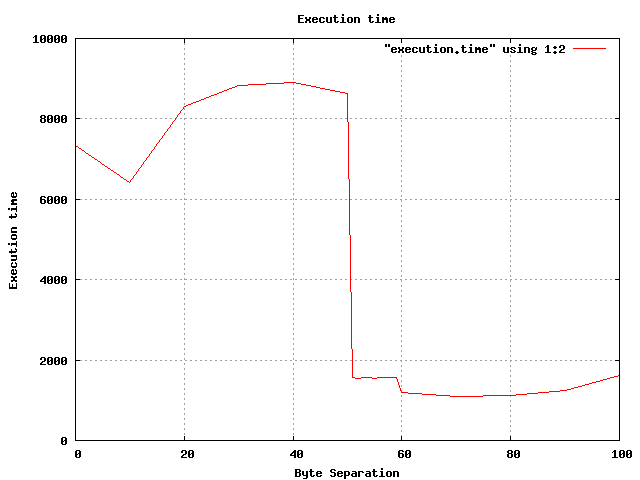
\includegraphics[width=0.6\textwidth]{images/falsesharing.png}\\
Execution time graph showing 5x speedup by ``wasting'' some space~\cite{falsesharing}.
\end{center}

At separation size 51 there is a huge drop in execution time because now we are certainly putting the two arrays in two locations that do not have the false sharing problem. Is wasting a little space worth it? Yes!

P.S. putting these arrays in a struct and padding the struct can also help with enabling future updates to the struct.

\subsection*{Volatile}

\begin{quote}
``Well, I read that {\tt volatile} variables aren't stored in registers,
    so then am I okay?''
\end{quote}

Again, sadly, no. Recall that {\tt volatile} in C was only designed to~\cite{pr:volatile}:
      \begin{itemize}
        \item Allow access to memory mapped devices.
        \item Allow uses of variables between {\tt setjmp} and {\tt longjmp}.
        \item Allow uses of {\tt sig\_atomic\_t} variables in signal handlers.
      \end{itemize}

All of these things apply to single-threaded situations or cases where the compiler has re-ordered some steps. Remember, things can also be reordered by the compiler, and {\tt
  volatile} doesn't prevent reordering. Also, it's likely your
variables could be in registers the majority of the time, except in
critical areas. All that volatile does is tell the compiler that an access of that variable should go to memory, not a register.









\chapter*{5 --- Concurrency and Parallelism}

\addcontentsline{toc}{chapter}{5 --- Concurrency and Parallelism}

\section*{Concurrency and Parallelism}
Concurrency and parallelism both give up the
total ordering between instructions in a sequential program, for
different purposes.

\paragraph{Concurrency.} We'll refer to the use of threads for
structuring programs as concurrency. Here, we're not aiming
for increased performance. Instead, we're trying to write the program
in a natural way. Concurrency makes sense as a model for distributed
systems, or systems where multiple components interact, with no ordering
between these components, like graphical user interfaces.

\paragraph{Parallelism.} We're studying parallelism in this class, where
we try to do multiple things at the same time in an attempt to increase
throughput. Concurrent programs may be easier to parallelize.

\subsection*{Limits to parallelization}
I mentioned briefly in Lecture 1 that programs often have a sequential
part and a parallel part. We'll quantify this observation today
and discuss its consequences.

\paragraph{Scalable Algorithms.} 
Remember from ECE~250/CS~138 that we often care about the worst case run-time performance of the algorithm. An algorithm that's $O(n^{3})$ scales so much worse than one that's $O(n)$ that it's not even funny. Trying to do an insertion sort on a small array is fine (actually... recommended); doing it on a huge array is madness. Choosing a good algorithm is very important if we want it to scale. 

\begin{center}
	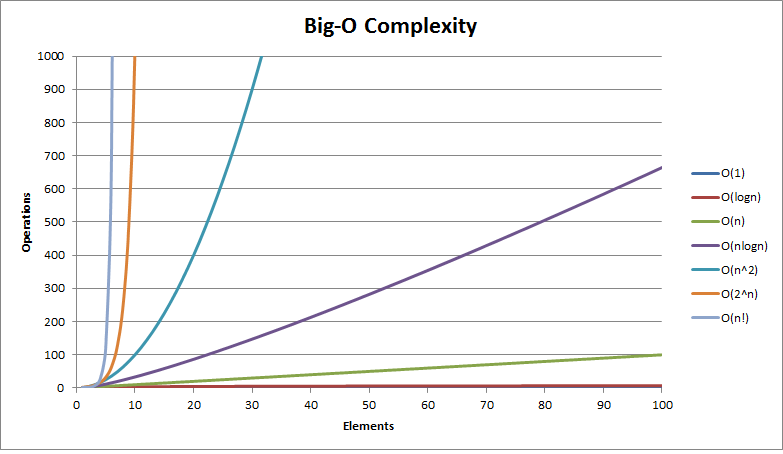
\includegraphics[width=0.75\textwidth]{images/big-o-complexity}\\
	Big-O Complexity comparison from ~\cite{bigocheatsheet}
\end{center}


\paragraph{Amdahl's Law.} One classic model of parallel execution
is Amdahl's Law. In 1967, Gene Amdahl argued that improvements in
processor design for single processors would be more effective than
designing multi-processor systems. Here's the argument. Let's say that
you are trying to run a task which has a serial part, taking fraction 
$S$, and a parallelizable part, taking fraction $P = 1-S$. Define $T_s$
to be the total 
amount of time needed on a single-processor system.
Now, moving to a parallel system with $N$ processors, the parallel
time $T_p$ is instead:
\[ T_p = T_s \cdot (S + \frac{P}{N}). \]
{\bf As $N$ increases, $T_p$ is dominated by $S$, limiting potential
speedup.}

We can restate this law in terms of speedup, which is the 
original time $T_s$ divided by the sped-up time $T_p$:
\[ \mbox{speedup} = \frac{T_s}{T_p} = \frac{1}{S+P/N}. \]
Replacing $S$ with $(1-P)$, we get:
\[ \mbox{speedup} = \frac{1}{(1-P)+P/N}, \]
and
\[ \mbox{max speedup} = \frac{1}{(1-P)}, \]
since $\frac{P}{N} \rightarrow 0$.

\paragraph{Plugging in numbers.} If $P = 1$, then we can indeed get good
scaling; running on an $N$-processor machine will give you a speedup
of $N$. Unfortunately, usually $P < 1$.  Let's see what happens.

\begin{center}
\begin{tabular}{r|r}
$P$ & speedup ($N=18$) \\ \hline
1 & 18 \\
0.99 & $\sim$ 15 \\
0.95 & $\sim$ 10 \\
0.5 & $\sim$ 2
\end{tabular}
\end{center}
Graphically, we have something like this:
\begin{center}
  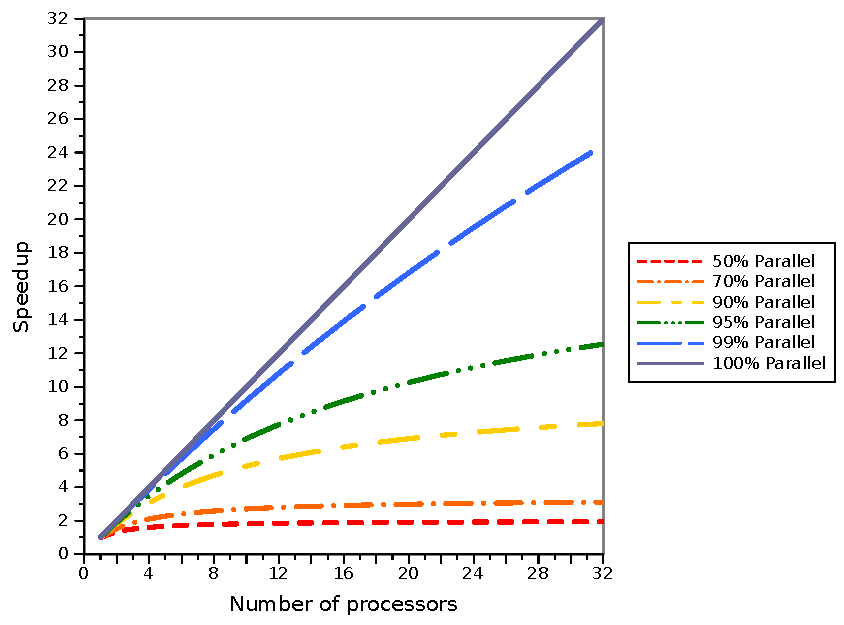
\includegraphics[width=0.5\textwidth]{images/parallel-scaling}
\end{center}


Amdahl's Law tells you how many cores you can hope to leverage in an
execution given a fixed problem size, if you can estimate $P$.

Let us consider an example from~\cite{mte241}: Suppose we have a task that can be executed in 5~s and this task contains a loop that can be parallelized. Let us also say initialization and recombination code in this routine requires 400~ms. So with one processor executing, it would take about 4.6~s to execute the loop. If we split it up and execute on two processors it will take about 2.3~s to execute the loop. Add to that the setup and cleanup time of 0.4~s and we get a total time of 2.7~s. Completing the task in 2.7~s rather than 5~s represents a speedup of about~46\%. Applying the formula, we get the following run times:

\begin{center}
	\begin{tabular}{l|l}
	\textbf{Processors} & \textbf{Run Time (s)} \\ \hline
	1 & 5\\
	2 & 2.7\\
	4 & 1.55\\
	8 & 0.975\\
	16 & 0.6875 \\
	32 & 0.54375 \\
	64 & 0.471875 \\
	128 & 0.4359375\\
	\end{tabular}
\end{center}

   \paragraph{Empirically estimating parallel speedup $P$.}
Assuming that you know things that are actually really hard to know, here's a formula for estimating speedup. You don't have to commit it to memory:
  \[P_{\mbox{\scriptsize estimated}} = \frac{\frac{1}{\mbox{\em speedup}}-1}{\frac{1}{N}-1}.\]

It's just an estimation, but you can use it to guess the fraction of parallel code, given $N$ and the speedup. You can then use $P_{\mbox{\scriptsize estimated}}$ to predict speedup for a different number of processors.

\paragraph{Consequences of Amdahl's Law.}
For over 30 years, most performance gains did indeed come from
increasing single-processor performance. The main reason that we're
here today is that, as we saw last time,
single-processor performance gains have hit the wall.

By the way, note that we didn't talk about the cost of synchronization
between threads here. That can drag the performance down even more.

\paragraph{Amdahl's Assumptions.}
Despite Amdahl's pessimism, we still all have multicore computers today.
Why is that? Amdahl's Law assumes that:
\begin{itemize}[noitemsep]
    \item problem size is fixed (read on);
    \item the program, or the underlying implementation, behaves the same on 1 processor as on $N$ processors; and
    \item that we can accurately measure runtimes---i.e. that overheads don't matter.
\end{itemize}

% replace Amdahl's law with how branch predictors work
%% \paragraph{Generalizing Amdahl's Law.} We made a simplification,
%% which was that programs only have one parallel part and one serial part.
%% Of course, this is not true. The program may have many parts,
%% each of which we can tune to a different degree.

%% Let's generalize Amdahl's Law:

%% \begin{itemize}
%% \item  $f_1, f_2, \ldots, f_n$: fraction of time in part $n$
%% \item  $S_{f_1}, S_{f_n}, \ldots, S_{f_n}$: speedup for part $n$
%% \end{itemize}

%% Then,
%% \[\mbox{\em speedup} = \frac{1}{\frac{f_1}{S_{f_1}} + \frac{f_2}{S_{f_2}} + \ldots +
%%     \frac{f_n}{S_{f_n}}}.\]

%% \paragraph{Example.} Consider a program with 4 parts in the following scenario:

%% \begin{center}
%%     \begin{tabular}{r|r|r|r}
%%     \multicolumn{2}{l}{} & \multicolumn{2}{|c}{Speedup} \\
%%     Part & Fraction of Runtime & Option 1 & Option 2\\
%%     \hline
%%     1 & 0.55 & 1  & 2\\
%%     2 & 0.25 & 5  & 1\\
%%     3 & 0.15 & 3  & 1\\
%%     4 & 0.05  & 10 & 1\\
%%     \end{tabular}
%% \end{center}

%%     (Note: these speedups don't have to be speedups from parallelization.)
    
%%   We can implement either Option 1 or Option 2. 
%%   Which option is better?

%%   ``Plug and chug'' the numbers:
%% \begin{itemize}
%% \item  {\bf Option 1.}

%%   \[ \mbox{\em speedup} = \frac{1}{0.55 + \frac{0.25}{5} + \frac{0.15}{3} + \frac{0.05}{5}}
%%     = 1.53  \]

%% \item  {\bf Option 2.}

%%   \[\mbox{\em speedup} = \frac{1}{\frac{0.55}{2} + 0.45} = 1.38 \hspace*{5.5em}\]
%% \end{itemize}

\subsection*{A more optimistic point of view}
In 1988, John Gustafson pointed
out\footnote{\url{http://www.scl.ameslab.gov/Publications/Gus/AmdahlsLaw/Amdahls.html}}
that Amdahl's Law only applies to fixed-size problems, but that the
point of computers is to deal with bigger and bigger problems.

In particular, you might vary the input size, or the grid resolution,
number of timesteps, etc. When running the software, then, you might
need to hold the running time constant, not the problem size: you're
willing to wait, say, 10 hours for your task to finish, but not 500
hours. So you can change the question to: how big a problem can you
run in 10 hours?

According to Gustafson, scaling up the problem tends to increase the
amount of work in the parallel part of the code, while leaving the
serial part alone. As long as the algorithm is linear, it is possible
to handle linearly larger problems with a linearly larger number of
processors.

Of course, Gustafson's Law works when there is some ``problem-size''
knob you can crank up.  As a practical example, observe Google, which
deals with huge datasets.


\section*{Software Design Issues}


\paragraph{Locking.}
Think back to a concurrency course and the discussion of locking. We'll be coming back to this subject before too long. But for now, suffice it to say, that the more locks and locking we need, the less scalable the code is going to be. You may think of the lock as a resource and the more threads or processes that are looking to acquire that lock, the more ``resource contention'' we have, and the more waiting and coordination are going to be necessary.

\paragraph{Memory Allocators.}
Assuming we're not working with an embedded system where all memory is statically allocated in advance, there will be dynamic memory allocation. The memory allocator is often centralized and may support only one thread allocating or deallocating at a time. This means it does not necessarily scale very well. There are, however, some techniques for dynamic memory allocation that allow these things to work in parallel.

\paragraph{Pools of Worker Threads.}
We'll talk about threads shortly. At first, one might imagine manually starting the necessary threads. But that's not the only way. We can have a pool of workers. Then the application just submits units of work, and then on the other side these units of work are allocated to workers. The number of workers will scale based on the available hardware. This is neat as a programming practice: as the application developer we don't care quite so much about the underlying hardware. Let the operating system decide how many workers there should be, to figure out the optimal way to process the units of work.

\section*{Processes and Threads} Let's review the
difference between a process and a thread. A \emph{process} is an
instance of a computer program that contains program code and its own
address space, stack, registers, and resources (file handles, etc).  A
\emph{thread} usually belongs to a process. The most important point
is that it shares an address space with its parent process, hence
variables and code as well as resources. Each thread has its own~\cite{osi}:
\begin{enumerate}
	\item Thread execution state (like process state: running, ready, blocked...).
	\item Saved thread context when not running.
	\item Execution stack.
	\item Local variables.
	\item Access to the memory and resources of the process (shared with all threads in that process).
\end{enumerate}

Or, to represent this visually:

\begin{center}
	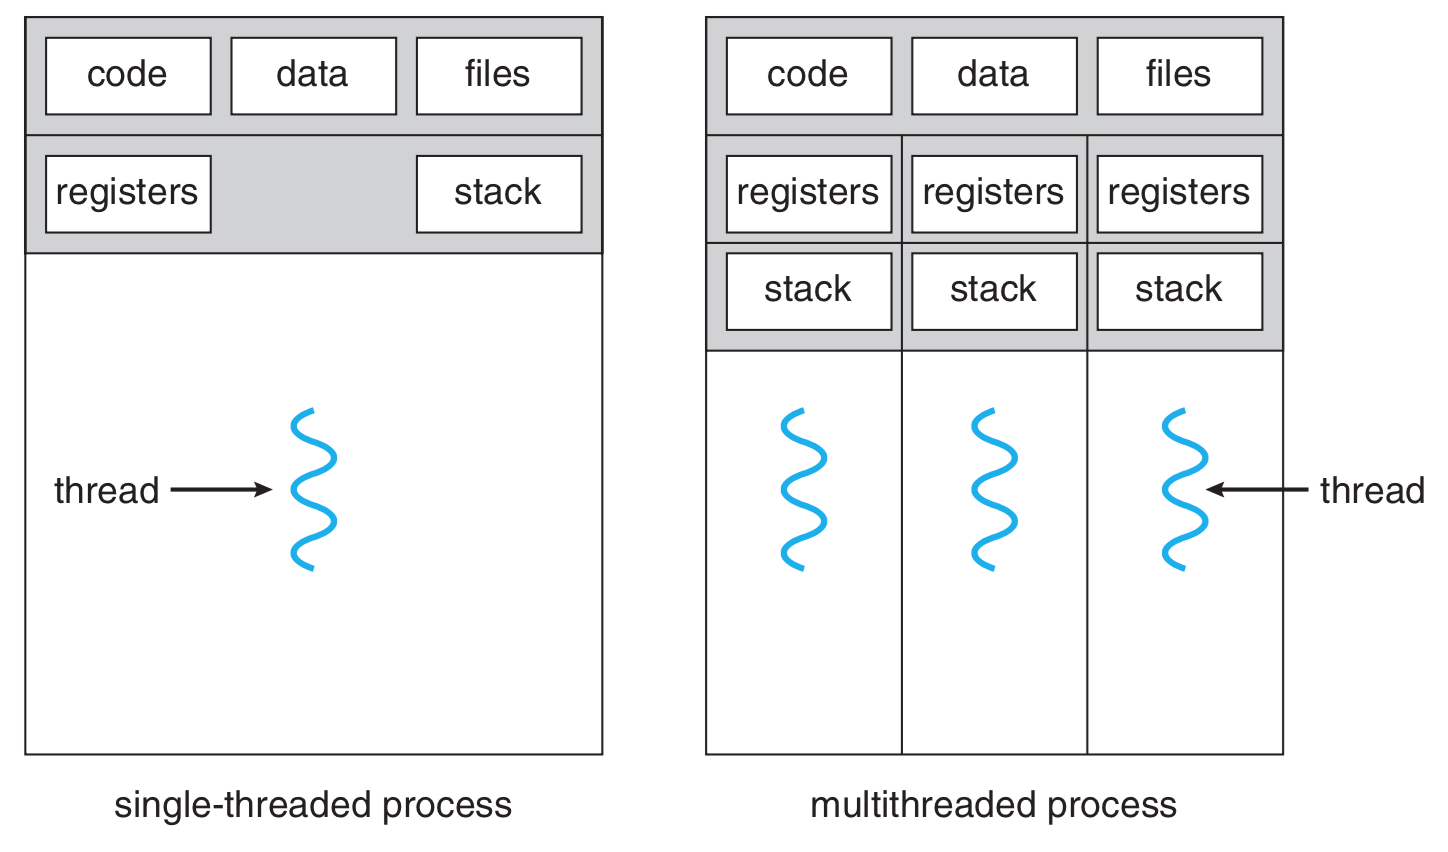
\includegraphics[width=0.6\textwidth]{images/mthread2.png}\\
	A single threaded and a multithreaded process compared side-by-side~\cite{osc}.
\end{center}

All the threads of a process share the state and resources of the process. If one thread opens a file, other threads in that process can also access that file.

The way programs are written now, there are few, if any, that are not in some way multithreaded. One common way of dividing up the program into threads is to separate the user interface from a time-consuming action.

Consider a file-transfer program. If the user interface and upload method share a thread, once a file upload has started, the user will not be able to use the UI anymore (and Windows will put the dreaded ``(Not Responding)'' at the end of its dialog title), even to click the button that cancels the upload. For some reason, users hate that. 

We have two options for how to alleviate this problem: when an upload is ready to start, we can call \texttt{fork} and create a new process to do the upload, or we can spawn a new thread. In either case, the newly created entity will handle the upload of the file. The UI remains responsive, because the UI thread is not waiting for the upload method to complete.

\subsection*{Motivation for Threads}

Why choose threads rather than creating a new process? The primary, but not sole, motivation is performance:
\begin{enumerate}
	\item Creating a new thread is much faster than creating a new process. In fact, thread creation is on the order of ten times faster~\cite{machThreads}.
	\item Terminating and cleaning up a thread is faster than terminating and cleaning up a process.
	\item It takes less time to switch between two threads within the same process (because less data needs to be stored/restored). In Solaris, for example, switching between processes is about five times slower than switching between threads~\cite{osc}.
	\item Because threads share the same memory space, for two threads to communicate, they do not have to use any of the IPC mechanisms; they can just communicate directly.
	\item As in the file transfer program, use of threads allows the program to be responsive even when a part of the program is blocked.
\end{enumerate}

This last advantage, background work, is one of four common examples of the uses of threads in a general purpose operating system~\cite{insideOS2}:
\begin{enumerate}
	\item \textbf{Foreground and Background Work:} as already examined, the ability to run something in the background to keep the program responsive.
	\item \textbf{Asynchronous processing}: for example, to protect against power failure or a crash, a word processor may write the document data in main memory to disk periodically. This can be done as a background task so it does not disrupt the user's workflow.
	\item \textbf{Speed of Execution:} a multithreaded program can get more done in the same amount of time. Just as the OS can run a different program when the executing program gets blocked (say, on a disk read), if one thread is blocked, another thread may execute.
	\item \textbf{Modular Structure:} a program that does several different things may be given structure through threads.
\end{enumerate}

There are some drawbacks, however: there is no protection between threads in the same process. So, one thread can easily mess with the memory being used by another thread. This once again brings us to the subject of co-ordination, which will follow the discussion of threads.

Also, if any thread encounters an error (such as a division by zero or Segmentation Fault), the whole process might be terminated by the operating system. If the program has multiple processes for different parts, then the other processes will not be affected. But, if the program has multiple threads and they all share the same process, then any thread encountering an error might bring all of them to a halt. (That's why Google Chrome chose to use separate processes for each tab.)



You can find another explanation of processes versus threads here:
\begin{center}
  \url{https://www.purplealienplanet.com/node/50}
\end{center}

\paragraph{Threads and CPUs.} In your operating systems class,
you've seen implementations of threads (``lightweight processes'').
We'll call these threads \emph{software threads}, and we'll program
with them throughout the class. Each software thread corresponds to a
stream of instructions that the processor executes. On a old-school
single-core, single-processor machine, the operating system
multiplexes the CPU resources to execute multiple threads
concurrently; however, only one thread runs at a time on the single
CPU.

On the other hand, a modern chip contains a number of \emph{hardware
threads}, which correspond to the virtual CPUs. These are sometimes
known as \emph{strands}. The operating system still needs to 
multiplex the software threads onto the hardware threads, but now has
more than one hardware thread to schedule work onto.



\paragraph{Implementing (or Simulating) Hardware Threads.} 
There are a number of ways to implement multiple software threads; for
instance, the simplest possible implementation, {\bf kernel-level
threading} (or 1:1 model) dedicates one core to each thread. The kernel schedules threads
on different processors. (Note that kernel involvement will always be required to
take advantage of a multicore system). This model is used by Win32, as well as
POSIX threads for Windows and Linux. The 1:1 model allows concurrency and parallelism.

Alternately, we could make one core execute multiple threads. In the
{\bf user-level threading}, or N:1, model, the single core would keep
multiple contexts and could 1) switch every 100 cycles; 2) switch
every cycle; 3) fetch one instruction from each thread each cycle; or
4) switch every time the current thread hits a long-latency event
(cache miss, etc.) This model allows for quick context switches, but
does not leverage multiple processors. (Why would you use these?) The N:1 model is used by
GNU Portable Threads.

Finally, it's possible to both use multiple cores and put multiple
threads onto one core, in a {\bf hybrid threading}, or M:N, model. Here, we map $M$ application threads to $N$ kernel threads. This
is a compromise between the previous two models, which both allows
quick context switches and the use of multiple processors. However, it
requires increased complexity; the library provides scheduling
services, which may not coordinate well with kernel, and increases
likelihood of priority inversion (which you've seen in Operating
Systems).  This method is used by modern Windows threads.


\section*{Choose Your Pain}
The first design decision that you need to solve when parallelizing programs
is whether you should use threads or processes.

  \begin{itemize}
    \item Threads are basically light-weight processes which piggy-back on
          processes' address space.
  \end{itemize}

Traditionally (pre-Linux 2.6) you had to use {\tt
  fork}~(for~processes) and {\tt clone} (for threads). But {\tt clone}
is not POSIX compliant, and its man page says that it's
Linux-specific---FreeBSD uses {\tt rfork()}. (POSIX is the standard
for Unix-like operating systems).

\paragraph{When processes are better.} {\tt fork} is safer and more secure than threads.

  \begin{enumerate}
    \item Each process has its own virtual address space:
      \begin{itemize}
        \item Memory pages are not copied, they are copy-on-write. Therefore, processes use less memory than you would expect.
      \end{itemize}
    \item Buffer overruns or other security holes do not expose other~processes.
    \item If a process crashes, the others can continue.
  \end{enumerate}

{\bf Example:} In the Chrome browser, each tab is a separate
process. Scott McCloud explained this:
\url{http://www.scottmccloud.com/googlechrome/}.

\paragraph{When threads are better.} Threads are easier and faster.

  \begin{enumerate}
    \item Interprocess communication (IPC) is more complicated and slower than interthread
          communication; must use operating system utilities (pipes, semaphores, shared
              memory, etc) instead of thread library (or just memory reads and writes).
    \item Processes have much higher startup, shutdown, and synchronization costs than threads.
    \item pthreads fix the issues of {\tt clone} and provide a
          uniform interface for most systems. (You'll work with them in Assignment 1.)
  \end{enumerate}

\paragraph{How to choose?}
  If your application is like this:
  \begin{itemize}
    \item mostly independent tasks, with little or no communication;
    \item task startup and shutdown costs are negligible compared to overall runtime; and
    \item want to be safer against bugs and security holes,
  \end{itemize}
then processes are the way to go. If it's the opposite of this, then use threads.

For performance reasons, along with ease and consistency across systems, we'll use threads. We will describe both pthreads and C++ 11 threads, in particular.

\paragraph{Overhead of Processes vs Threads.} The common wisdom is that processes are
expensive, threads are cheap. Let's verify this with a benchmark on a
laptop (included in the live-coding directory on GitHub) which creates and destroys 50,000 threads:
  \begin{lstlisting}[basicstyle=\scriptsize]
jon@riker examples master % time ./create_fork 
0.18s user 4.14s system 34% cpu 12.484 total
jon@riker examples master % time ./create_pthread 
0.73s user 1.29s system 107% cpu 1.887 total
  \end{lstlisting}

Clearly pthreads incur much lower overhead than {\tt fork}. pthreads
offer a speedup of 6.5 over processes in terms of startup and teardown costs.

%\paragraph{Live Coding Example.} We can write a program to determine
%whether we are in a user-level threading model vs. the other two models.
%Just start a child thread and make both threads compute. If CPU utilization
%exceeds 100\%, we are not user-level threading. The example I saw in class
%computes $2^{28}$ random numbers to spin the CPU.

%(Is it possible to differentiate hybrid and kernel threading by writing a
%simple program?)












\chapter*{6 --- Working with Threads}

\addcontentsline{toc}{chapter}{6 --- Working with Threads}

\section*{Using Threads to Program for Performance}
We'll start by seeing how to use threads on ``embarrassingly parallel problems'', which have mostly-independent sub-problems (little synchronization) and strong locality (little communication). Later, we'll see which problems are amenable to parallelization (\emph{dependencies}) and alternative parallelization patterns (right now, just use one thread per sub-problem).

\paragraph{About pthreads.} pthreads stands for POSIX threads. It's available
on most systems, including pthreads Win32 (which I don't recommend).
Use Linux, and our provided server, for this course. \CPP 11 also includes threads
in its specification.

For your convenience, the function signatures of the relevant pthread calls is shown below. We'll assume you used them to at least some extent in a previous context. If this is new to you (for whatever reason), then look at the \texttt{pthreads.pdf} document in the course repository, where a quick summary of this material is provided~\cite{pthreads}.

\begin{lstlisting}[language=C]
pthread_create( pthread_t *thread, const pthread_attr_t *attributes,
                void *(*start_routine)( void * ), void *argument )
pthread_join( pthread_t thread, void **return_value )
pthread_detach( pthread_t thread )
pthread_cancel( pthread_t thread )
pthread_testcancel( ) /* If the thread is cancelled, this function does not return (thread terminated) */
pthread_exit( void *value )
\end{lstlisting}

To compile a C or \CPP program with threads, add the {\tt -pthread}
parameter to the compiler commandline. Old compilers might complain
because they default to a too-old C. Starting with {\tt gcc} 5, the
GCC C compiler will always default to at least C11. {\tt g++} 5
defaults to \CPP 98, while 6 and up default to at least \CPP 14. To
ensure C99 support even with old GCCs, add \texttt{-std=c99} to the
commandline. To ensure \CPP11 support in GCC, use \verb!-std=C++11!.

%% FYI:
%% gcc 8:
%% C: C17
%% C++: C++ 14

%% gcc 6-7:
%% C: C11
%% C++: C++ 14

%% gcc 5:
%% C: C11
%% C++: C++98

\paragraph{Starting a new thread.} You can start a thread with
\verb+pthread_create()+ or by creating a \verb+std::thread+:

{\small
  \begin{minipage}{.55\textwidth}
\begin{lstlisting}[language=C]
#include <pthread.h>
#include <stdio.h>

void* run(void*) {
  printf("In run\n");
}

int main() {
  pthread_t thread;
  pthread_create(&thread, NULL, run, NULL);
  printf("In main\n");
}
\end{lstlisting}
  \end{minipage} 
  \begin{minipage}{.4\textwidth}
\begin{lstlisting}[language=C]
#include <thread>
#include <iostream>

void run() {
  std::cout << "In run\n";
}

int main() {
  std::thread t1(run);
  std::cout << "In main\n";
  t1.join(); // see below
}
\end{lstlisting}
  \end{minipage}
}

\paragraph{Attributes.} In previous courses, you were probably told that the default attributes would be fine. And generally they are\ldots if it is a first concurrency course! But in a more advanced context, we may need to pay attention to the attributes. The most salient thread attribute that was previously discussed was about whether a thread was detached (i.e., not joinable).

Beyond being detached/joinable, threads have additional
attributes. (Note, also, that even though being joinable rather than
detached is the default on Linux, it's not necessarily the default everywhere).
Here's a list.
  \begin{itemize}
    \item Detached or joinable state
    \item Scheduling inheritance
    \item Scheduling policy
    \item Scheduling parameters
    \item Scheduling contention scope
    \item Stack size
    \item Stack address
    \item Stack guard (overflow) size
  \end{itemize}

Basically, you create and destroy attributes objects with {\tt
  pthread\_attr\_init} and {\tt pthread\_attr\_destroy}
respectively. You can pass attributes objects to {\tt
  pthread\_create}. For instance,

  \begin{lstlisting}[language=C]
size_t stacksize;
pthread_attr_t attributes;
pthread_attr_init(&attributes);
pthread_attr_getstacksize(&attributes, &stacksize);
printf("Stack size = %i\n", stacksize);
pthread_attr_destroy(&attributes);
  \end{lstlisting}

Running this on a laptop produces:

  \begin{lstlisting}[language=C]
jon@riker examples master % ./stack_size 
Stack size = 8388608
  \end{lstlisting}
  
Obviously, stack size is not the only attribute you can check. The pthread library contains a lengthy listing of all the get-this and get-that functions that define how to read the value of a particular attribute. If you are curious! And along with get-functions there are naturally set-functions as well.

Once you have a thread attribute object, you can set the thread state to joinable:
  \begin{lstlisting}[language=C]
pthread_attr_setdetachstate(&attributes, PTHREAD_CREATE_JOINABLE);
  \end{lstlisting}

 

\subsection*{Things Fall Apart}
Okay, so you should be at least somewhat familiar with basic thread usage. But unfortunately there are some number of pitfalls that we need to avoid. These may have a negative impact on the correctness or the performance of your program.


\paragraph{Stack Allocation.} Recall that the {\tt pthread\_create} 
call allows you to pass data to the new thread. Let's see how we might do that\ldots

\begin{lstlisting}[language=C]
int i;
for (i = 0; i < 10; ++i) {
  pthread_create(&thread[i], NULL, run, &i);
}
\end{lstlisting}

{\bf Wrong!} This is a \emph{terrible} idea. Why?
\begin{enumerate}
    \item The value of {\tt i} will probably change before the thread executes.
    \item The memory for {\tt i} may be out of scope, and therefore invalid by
          the time the thread executes.
\end{enumerate}
The worst part is that in a simple program where you just write most of the pthread launch logic in main, then \texttt{i} will not go out of scope and it will seem like everything is fine\ldots Instead we need to do this:

\begin{lstlisting}[language=C]
int i;
int* arg;
for (i = 0; i < 10; ++i) {
  arg = malloc( sizeof( int ) );
  *arg = i;
  pthread_create(&thread[i], NULL, run, arg);
}
\end{lstlisting}

And then \texttt{arg} needs to be deallocated at some point by the thread.

On the other hand, you can pull off something similar with \CPP11 threads:
\begin{lstlisting}[language=C]
int i;
for (i = 0; i < 10; ++i) {
  std::thread t(run, i);
  t.detach();
}
\end{lstlisting}
This is OK because we pass {\tt i} by value, which doesn't work for pthreads.

In pthreads-land, you might be able to get away with this.
\begin{lstlisting}[language=C]
int i;
for (i = 0; i < 10; ++i)
  pthread_create(&thread[i], NULL, &run, (void*)i);

...

void* run(void* arg) {
  int id = (int)arg;
\end{lstlisting}
It's not ideal, though. We're abusing the pointer by storing a number in it. Which might work, but you do have to be careful. Beware size mismatches between arguments: you have no guarantee that a pointer is the same size as an int, so your data may overflow. And, sizes of data types change between systems. For maximum portability, just use pointers you got from {\tt malloc}.


\paragraph{Libraries} Make sure the libraries you use are {\bf thread-safe}: the library protects its shared data (i.e., can be called by more than one thread concurrently). We'll get into this in some more detail later.

How do you know if a function is thread safe? If you wrote it yourself or have the source code, you could take a look. But for an arbitrary library the best way to know is\ldots read the documentation. No! Anything but that!!!

The glibc reentrant functions are also safe: a program can have
      more than one thread calling these functions concurrently. For
      example, use {\tt rand\_r}, not {\tt rand}.


\paragraph{Catch You Later\ldots}Joinable threads
(which is the default on Linux) wait for someone to call {\tt pthread\_join}
before they release their resources (e.g. thread stacks). On the other
hand, you can also create \emph{detached} threads, which release
resources when they terminate, without being joined. 

It is good practice to detach a thread using \texttt{pthread\_detach} if you have no intention of joining it ever. Otherwise the memory and resources allocated to this thread might hang around for the whole execution of your program. Be polite and clean these up sooner! 

Calling {\tt pthread\_detach} on an already detached thread results in undefined behaviour. If we try to join a thread that's detached, it's also undefined behaviour. In a live coding demo I found that the program didn't crash if the join call used \texttt{NULL} as the second argument (i.e., we were not trying to collect any value), but things got weird quickly if we did try to get a return value out of it. Better not to do this.


  The idiomatic way of returning data from threads in \CPP11 appears to be using
  futures. {\tt std::async} provides support for this:
\begin{lstlisting}[language=C]
#include <thread>
#include <iostream>
#include <future>

int run() {
  return 42;
}

int main() {
  std::future<int> t1_retval = std::async(std::launch::async, run);
  std::cout << t1_retval.get();
}
\end{lstlisting}
This launches your thread for you. The {\tt get()} call waits until the answer
is ready and returns it to you.

Consider also the following small danger of detached threads:

\begin{lstlisting}[language=C]
#include <pthread.h>
#include <stdio.h>

void* run(void*) {
  printf("In run\n");
}

int main() {
  pthread_t thread;
  pthread_create(&thread, NULL, &run, NULL);
  pthread_detach(thread);
  printf("In main\n");
}
\end{lstlisting}

  When I run it, it just prints ``In main''. Why?

\paragraph{Solution.} Use {\tt pthread\_exit} to quit if you have any detached threads.
  \begin{lstlisting}[language=C]
#include <pthread.h>
#include <stdio.h>

void* run(void*) {
  printf("In run\n");
}

int main() {
  pthread_t thread;
  pthread_create(&thread, NULL, &run, NULL);
  pthread_detach(thread);
  printf("In main\n");
  pthread_exit(NULL); // This waits for all detached
                      // threads to terminate
}
  \end{lstlisting}
(There is no \CPP11 equivalent.)

\paragraph{Finishing a thread.} The typical way to end a thread is via the \texttt{pthread\_exit} call with a pointer to the return value (if any is desired). On some systems, though, this results in reported memory leaks. Well, nobody says the authors of the thread libraries are perfect. Returning from the thread's {\tt start\_routine} via a \texttt{return} statement is equivalent to calling {\tt pthread\_exit}, and {\tt start\_routine}'s return value is passed back to the {\tt pthread\_join} caller. That may work better for you. There is no \CPP11 equivalent.



\paragraph{Now's not a good time!} You may also recall that threads can be terminated using cancellation, which may be asynchronous (immediate death) or synchronous (a thread terminates when it gets to a cancellation point). Sometimes a thread can be terminated before it has cleaned up some resources. This is undesirable. One way that we can guard against this is to register cleanup handlers for that thread. If, say, our thread allocated some memory, it would be wise to register a cleanup handler that deallocates that memory in case the thread should die unceremoniously. The function signatures are:

\begin{lstlisting}[language=C]
pthread_cleanup_push( void (*routine)(void*), void *argument ); /* Register cleanup handler, with argument */ 
pthread_cleanup_pop( int execute ); /* Run if execute is non-zero */ 
\end{lstlisting}

To add a cleanup handler, the push function is used. Its two arguments are the function that is supposed to run, and a pointer to the argument that cleanup function will need.

The push function always needs to be paired with the pop function at the same level in your program (where level is defined by the curly braces). You should think of them as being like the opening curly brace at the start of a statement and the closing curly brace at the end; they have to be correctly matched up. The pop function takes one argument: whether it should run or not. If the thread is cancelled, the cleanup function will run; if it continues to the pop function, then you get to choose whether it runs or not.

Consider the following code: 
\begin{lstlisting}[language=C]
void* do_work( void* argument ) {
  struct job * j = malloc( sizeof( struct job ) );
  /* Do something useful with this structure */
  /* Actual work to do not shown */
  free( j );
  pthread_exit( NULL );
\end{lstlisting}

Suppose that the thread is cancelled during the block operating on \texttt{j} and it is set up for asynchronous cancellation. This means that the code will never get to the \texttt{free()} call, which means that the memory allocated at the beginning is leaked! We can remedy this with application of a cleanup handler:
\begin{lstlisting}[language=C]
void cleanup( void* mem ) {
  free( mem );
}

void* do_work( void* argument ) {
  struct job * j = malloc( sizeof( struct job ) );
  pthread_cleanup_push( cleanup, j );
  /* Do something useful with this structure */
  /* Actual work to do not shown */
  free( j );
  pthread_cleanup_pop( 0 ); /* Don't run */
  pthread_exit( NULL );
\end{lstlisting}



\subsection*{Advanced pthread calls} Here's a couple more advanced pthread function calls that are available for our use~\cite{pthreads}:

\begin{lstlisting}[language=C]
pthread_t pthread_self( void );
int pthread_equal( pthread_t t1, pthread_t t2 );
int pthread_once(pthread_once_t* once_control, void (*init_routine)(void));
pthread_once_t once_control = PTHREAD_ONCE_INIT;
\end{lstlisting}

The call to \texttt{pthread\_self} is a way to get a reference to the \texttt{pthread\_t} structure of the currently operating thread while it's running! This is distinct from the idea of calling \texttt{gettid()} which tells you the kernel thread number of a given thread. But even so, having the number would not be helpful as pretty much all the pthread function calls operate on the \texttt{pthread\_t} structure.

Unfortunately, the regular equality operator (\texttt{==}) can't be reliably used on a \texttt{pthread\_t} structure, so there exists a separate equality test. Strangely, though, it does the opposite of what you might expect in Java or similar: if the two thread IDs are equal, \texttt{pthread\_equal}returns a nonzero value; otherwise 0. So here 0 means non-equal. Sigh.

The last function and macro are about things you want to happen once but only once, no matter how many threads are started. The control variable is presumably global, and the first time that a thread calls the \texttt{pthread\_once} function, then the \texttt{init\_routine} function runs. On all later invocations, it does not. On return from \texttt{pthread\_once}, it is guaranteed that the initialization routine has finished executing.









\chapter*{7 --- Race Conditions \& Synchronization}

\addcontentsline{toc}{chapter}{7 --- Race Conditions \& Synchronization}


\section*{Race Conditions}
Previous courses (ECE~254 or equivalent) should have introduced the concept of a race condition. We'll be talking about them in greater detail in this course.

\begin{quote}
\textit{
	``Knock knock.''\\
	``Race Condition.''\\
	``Who's there?''
	}
\end{quote}

\paragraph{Definition.} A race occurs when you have two concurrent accesses to the
same memory location, at least one of which is a {\bf write}. In earlier courses you probably just considered any shared accesses or shared data at all. 

This definition is a little bit strict. We could also say that there is a race condition if there is some form of output, such as writing to the console. It's a write, but not necessarily to the same location. If one thread is going to write ``1'' to the console and another is going to write ``2'', then we could have a race condition. If there is no co-ordination, we could get output of ``12'' or ``21''. If the order here is unimportant, there's no issue; but if one order is correct, then the appearance of the other is a bug.

When there's a race, the final state may not be the same as running
one access to completion and then the other. But it ``usually'' is. It's nondeterministic. The fact that the output is often ``12'' and only very occasionally ``21'' may make it very difficult to track down the source of the problem. Furthermore, if we end up adding additional logging statements or use the debugger or anything to that effect, we will change the timing and possibly suppress (cover up) the behaviour of the bug.

\paragraph{Dependencies.}
Let's now consider two sequential operations that we would like to execute in parallel.
In other situations (e.g., processor design) we might say that there are dependencies between the operations. The problem is that we have something that needs to wait for something else. There are four basic possibilities to consider:

\begin{enumerate}
	\item \textbf{RAW} (Read After Write) - The classic form of dependency. The read has to take place after the write, otherwise there's nothing to read, or an incorrect value will be read.
	\item \textbf{WAR} (Write After Read) - A write cannot take place until the read has happened, to ensure the read takes the correct value.
	\item \textbf{WAW} (Write After Write) - A write cannot take place because an earlier write needs to happen first. If we do them out of order, the final value may be out of date or otherwise incorrect.
	\item \textbf{RAR} (Read After Read) - No such hazard! 
\end{enumerate}

\begin{center}
\begin{tabular}{l|ll}
& {\bf Read 2nd} & {\bf Write 2nd} \\ \hline
{\bf Read 1st} & Read after read (RAR) & Write after read (WAR) \\
& No dependency & Antidependency \\
{\bf Write 1st} & Read after write (RAW) & Write after write (WAW) \\
& True dependency & Output dependency
\end{tabular}
\end{center}

The no-dependency case (RAR) is clear. Declaring data immutable 
in your program is a good way to ensure no dependencies. In fact, making your data structures immutable is a good idea in general.


Race conditions typically arise between variables which are shared
between threads.

\paragraph{Example.}
\begin{multicols}{2}
\begin{lstlisting}[language=C]
#include <stdlib.h>
#include <stdio.h>
#include <pthread.h>

void* run1(void* arg){
    int* x = (int*) arg;
    *x += 1;
}

void* run2(void* arg){
    int* x = (int*) arg;
    *x += 2;
}
\end{lstlisting}
\columnbreak
\begin{lstlisting}[language=C]
int main(int argc, char *argv[]) {
    int* x = malloc(sizeof(int));
    *x = 1;
    pthread_t t1, t2;
    pthread_create(&t1, NULL, &run1, x);
    pthread_join(t1, NULL);
    pthread_create(&t2, NULL, &run2, x);
    pthread_join(t2, NULL);
    printf("%d\n", *x);
    free(x);
    return EXIT_SUCCESS;
}
\end{lstlisting}
\end{multicols}

\noindent
Question: Do we have a data race? Why or why not?
\vspace*{2em}
%No, we don't. Only one thread is active at a time.

\paragraph{Example 2.} Here's another example; keep the same thread definitions.
\begin{lstlisting}[language=C]
int main(int argc, char *argv[]) {
    int* x = malloc(sizeof(int));
    *x = 1;
    pthread_t t1, t2;
    pthread_create(&t1, NULL, &run1, x);
    pthread_create(&t2, NULL, &run2, x);
    pthread_join(t1, NULL);
    pthread_join(t2, NULL);
    printf("%d\n", *x);
    free(x);
    return EXIT_SUCCESS;
}
\end{lstlisting}

Now do we have a data race? Why or why not?
\vspace*{2em}

% Yes, we do. We have 2 threads concurrently accessing the same data.

\paragraph{Tracing our Example Data Race.} 
What are the possible outputs? (Assume that initially {\tt *x} is 1.)
We'll look at compiler intermediate code (three-address code) to tell.

\hspace*{.2\textwidth}\begin{minipage}{.8\textwidth}
\begin{lstlisting}[language=C]
run1                          run2   
D.1 = *x;                     D.1 = *x;
D.2 = D.1 + 1;                D.2 = D.1 + 2
*x = D.2;                     *x = D.2;
  \end{lstlisting}
\end{minipage}

Memory reads and writes are key in data~races.

Let's call the read and write from {\tt run1} R1 and W1; R2 and W2
from {\tt run2}. Assuming a sane\footnote{sequentially consistent; sadly, many
widely-used models are wilder than this.}
memory model, $R_n$ must precede $W_n$. {\bf C and \CPP do not guarantee
  such a memory model in the presence of races.} This reasoning would
actually only work if we declared {\tt x} as {\tt atomic} and did the
individual three-address code operations. Or, you could avoid this whole
mess by using read-modify-write instructions.

Here are all possible orderings:
  \begin{center}
    \begin{tabular}{llll|l}
\multicolumn{4}{c|}{Order} & {\tt *x}\\
\hline
R1 & W1 & R2 & W2 & 4 \\
R1 & R2 & W1 & W2 & 3 \\
R1 & R2 & W2 & W1 & 2 \\
R2 & W2 & R1 & W1 & 4 \\
R2 & R1 & W2 & W1 & 2 \\
R2 & R1 & W1 & W2 & 3 \\
    \end{tabular}
  \end{center}


Let's look at an antidependency (WAR) example.

{\small \begin{center}
\begin{tabular}{ll}
\begin{minipage}{.4\textwidth}
\begin{lstlisting}[language=C]
void antiDependency(int z) {
  int y = f(x);
  x = z + 1;
}
\end{lstlisting}
\end{minipage} &
\begin{minipage}{.4\textwidth}
\begin{lstlisting}[language=C]
void fixedAntiDependency(int z) {
  int x_copy = x;
  int y = f(x_copy);
  x = z + 1;
}
\end{lstlisting}
\end{minipage} 
\end{tabular}
\end{center} }
{\sf Why is there a problem?}\\[2em]

Finally, WAWs can also inhibit parallelization:

{\small \begin{center}
\begin{tabular}{ll}
\begin{minipage}{.45\textwidth}
\begin{lstlisting}[language=C]
void outputDependency(int x, int z) {
  y = x + 1;
  y = z + 1;
}
\end{lstlisting}
\end{minipage} &
\begin{minipage}{.4\textwidth}
\begin{lstlisting}[language=C]
void fixedOutputDependency(int x, int z) {
  y_copy = x + 1;
  y = z + 1;
}
\end{lstlisting}
\end{minipage} 
\end{tabular}
\end{center} }

In both of these cases, renaming or copying data can
eliminate the dependence and enable parallelization. Of course,
copying data also takes time and uses cache, so it's not free. One
might change the output locations of both statements and then copy in
the correct output. These are usually more useful when it's not just one
access, but some sort of longer computation.




\section*{Synchronization}
You'll need some sort of synchronization to get sane results from
multithreaded programs. We'll start by talking about how to use
mutual exclusion a bit. In a previous course you should have learned about semaphores at least, and hopefully a mutex as well. If not, you should take a look at the file \texttt{synchronization.pdf} in the course repository as it contains a nice recap of the basics. 


\paragraph{Mutual Exclusion.} Mutexes are an extremely common form of synchronization. When used properly, only one thread can access code protected by a mutex at a time; all other threads must wait until the mutex is free before they can execute the protected code.

Probably you have only used the pthread kind of mutex before. Here's a side by side comparison of the pthread mutex usage as well as the \CPP11:
    
    \begin{tabular}{ll}
      \begin{minipage}{.65\textwidth}
        {\bf pthreads}
  \begin{lstlisting}[language=C]
pthread_mutex_t m1_static = PTHREAD_MUTEX_INITIALIZER;
pthread_mutex_t m2_dynamic;

pthread_mutex_init(&m2_dynamic, NULL);
...
pthread_mutex_destroy(&m1_static);
pthread_mutex_destroy(&m2_dynamic);
  \end{lstlisting}
      \end{minipage}
      \begin{minipage}{.35\textwidth}
        {\bf \CPP11}
  \begin{lstlisting}[language=C]
mutex m1;
mutex * m2;

m2 = new mutex();
// ...

delete (m2);
  \end{lstlisting}
      \end{minipage}
    \end{tabular}

You can initialize mutexes statically (as with {\tt m1\_static}) or
dynamically ({\tt m2\_dynamic}). If you want to include attributes,
you need to use the dynamic version.

\paragraph{Mutex Attributes.} Mutexes use the notion of attributes.
We won't talk about mutex attributes in any detail, but here are the three standard ones. In previous courses we probably said just use \texttt{NULL} for the attributes and that's quite fine. But you might want some of these things:
  \begin{itemize}
    \item {\bf Protocol}: specifies the protocol used to prevent priority
      inversions for a mutex.
    \item {\bf Prioceiling}: specifies the priority ceiling of a mutex.
    \item {\bf Process-shared}: specifies the process sharing of a mutex.
  \end{itemize}
  You can specify a mutex as {\it process shared} so that you can access it
  between processes. In that case, you need to use shared memory and {\tt mmap},
  which we won't get into.

There is also the idea of trylock: you attempt to lock the mutex in a way that you won't get blocked whether we acquire the lock or not. The function returns a value to indicate if we succeeded and it is mandatory that we check. If successful, proceed; if unsuccessful then we'll have to try again at some point. Again, see the reference document if you need a recap of this.



\paragraph{My turn! No, my turn!} Key idea: locks protect resources; only one thread
can hold a lock at a time. A second thread trying to obtain the lock
(i.e. \emph{contending} for the lock) has to wait, or \emph{block},
until the first thread releases the lock. So only one thread has
access to the protected resource at a time. The code between the lock
acquisition and release is known as the \emph{critical region} or \emph{critical section}.

Excessive use of locks can serialize programs. Consider two resources
$A$ and $B$ protected by a single lock $\ell$. Then a thread that's
just interested in $B$ still has acquire $\ell$, which requires it to
wait for any other thread working with $A$. (The Linux kernel used to
rely on a Big Kernel Lock protecting lots of resources in the 2.0 era,
and Linux 2.2 improved performance on SMPs by cutting down on the use
of the BKL.) Mac OS also used to have problems with this, using the
big and small kernel locks (but this is something they got from us ing
the Mach microkernel, which is a whole other story.). We will come back to
the subject of how to avoid this problem soon.

Note: in Windows, the term ``mutex'' refers to an inter-process
communication mechanism. ``Critical sections'' are the mutexes we're
talking about above.

\paragraph{Spinlocks.} Spinlocks are a variant of mutexes, where the
waiting thread repeatedly tries to acquire the lock instead of sleeping.
Use spinlocks when you expect critical sections to finish 
quickly\footnote{For more information on spinlocks in the Linux
kernel, see \url{http://lkml.org/lkml/2003/6/14/146}.}. Spinning
for a long time consumes lots of CPU resources. Many lock
implementations use both sleeping and spinlocks: spin for a bit,
then sleep for longer. 

When would we ever want to use a spinlock? After all, we spend so much time talking about how we would never ever want to wait in a busy loop. Well. What we normally expect is to block until the lock becomes available. But that means a process switch, and then a switch back in the future when the lock is available. This takes nonzero time so it's optimal to use a spinlock if the amount of time we expect to wait for the lock is less than the amount of time it would take to do two process switches. As long as we have a multicore system.


\paragraph{Barriers.} This synchronization primitive allows you 
to make sure that a collection of threads all reach the
barrier before finishing. In pthreads, each thread should call
\verb+pthread_barrier_wait()+, which will proceed when enough threads
have reached the barrier. Enough means a number you specify upon
barrier creation.

\paragraph{Lock-Free Code.} We'll talk more about this soon.
Modern CPUs support atomic operations, such as compare-and-swap, which
enable experts to write lock-free code. A recent research 
result~\cite{mckenney11:_concur,Attiya:2011:LOE:1926385.1926442} states the requirements for correct implementations: basically,
such implementations must contain certain synchronization constructs.

\paragraph{Semaphores}
As you learned in previous courses, semaphores have a {\tt value} and
can be used for signalling between threads. When you create a semaphore,
you specify an initial value for that semaphore. Here's how they work.

This API is a lot like the mutex API:
  \begin{itemize}
    \item must link with {\tt -pthread} (or {\tt -lrt} on Solaris);
    \item all functions return {\tt 0} on success;
    \item same usage as mutexes in terms of passing pointers.
  \end{itemize}


\paragraph{Reader/Writer Locks.} Recall that data races only happen when
one of the concurrent accesses is a write. So, if you have read-only
(``immutable'') data, as often occurs in functional programs, you don't need
to protect access to that data. For instance, your program might
have an initialization phase, where you write some data, and then a 
query phase, where you use multiple threads to read the data.

Unfortunately, sometimes your data is not read-only. It might, for instance,
be rarely updated. Locking the data every time would be inefficient.
The answer is to instead use a \emph{reader/writer} lock.

\begin{enumerate}
\item Any number of readers may be in the critical section simultaneously.
\item Only one writer may be in the critical section (and when it is, no readers are allowed).
\end{enumerate}

Or, to sum that up, a writer cannot enter the critical section while any other thread (whether reader or writer) is there. While a writer is in the critical section, neither readers nor writers may enter the critical section~\cite{lbs}. This is very often how file systems work: a file may be read concurrently by any number of threads, but only one thread may write to it at a time (and to prevent reading of inconsistent data, no thread may read during the write).


The type for the lock is \texttt{pthread\_rwlock\_t}. It is analogous, obviously, to the mutex type \texttt{pthread\_mutex\_t}. Let's consider the functions that we have:

\begin{lstlisting}[language=C]
pthread_rwlock_init( pthread_rwlock_t * rwlock, pthread_rwlockattr_t * attr )
pthread_rwlock_rdlock( pthread_rwlock_t * rwlock )
pthread_rwlock_tryrdlock( pthread_rwlock_t * rwlock )
pthread_rwlock_wrlock( pthread_rwlock_t * rwlock )
pthread_rwlock_trywrlock( pthread_rwlock_t  *  rwlock )
pthread_rwlock_unlock( pthread_rwlock_t * rwlock )
pthread_rwlock_destroy( pthread_rwlock_t * rwlock )
\end{lstlisting}

In general our syntax very much resembles that of the mutex (attribute initialization and destruction not shown but they do exist). There are some small noteworthy differences, other than obviously the different type of the structure passed. Whereas before we had functions for lock and trylock, we now have those split into readlock and writelock (each of which has its own trylock function). As before, we will return to the subject of how trylock works soon.

In theory, the same thread may lock the same rwlock $n$ times; just remember to unlock it $n$ times as well.

And speaking of unlock, there's no specifying whether you are releasing a read or write lock. This is because it is unnecessary; the implementation unlocks whatever type the calling thread was holding. Much like \texttt{close()}, if we can figure out what we're closing we don't need the caller of the function to specify what to do.

As for whether readers get priority, the specification says this is implementation defined. If possible, for threads of equal priority, a writer takes precedence over a reader. But your system may vary.

Consider the following example of the simple readers-writers (without writer priority and with risk of starvation) using the ``old'' way:

\begin{multicols}{2}
\begin{lstlisting}[language=C]
int readers;
pthread_mutex_t mutex;
sem_t roomEmpty;

void init( ) {
  readers = 0;
  pthread_mutex_init( &mutex, NULL );
  sem_init( &roomEmpty, 0, 1 );
}

void cleanup( ) {
  pthread_mutex_destroy( &mutex );
  sem_destroy( &roomEmpty );
}
\end{lstlisting}

\columnbreak

\begin{lstlisting}[language=C]
void* writer( void* arg ) {
  sem_wait( &roomEmpty );
  write_data( arg );
  sem_post( &roomEmpty );
}

void* reader( void* read ) {
  pthread_mutex_lock( &mutex );
  readers++;
  if ( readers == 1 ) {
    sem_wait( &roomEmpty );
  }
  pthread_mutex_unlock( &mutex );
  read_data( arg );
  pthread_mutex_lock( &mutex );
  readers--;
  if ( readers == 0 ) {
    sem_post( &roomEmpty );
  }
  pthread_mutex_unlock( &mutex );
}
\end{lstlisting}

\end{multicols}

Now see it as it would be with the use of a rwlock!

\begin{multicols}{2}
\begin{lstlisting}[language=C]
pthread_rwlock_t rwlock;

void init( ) {
  pthread_rwlock_init( &rwlock, NULL );
}

void cleanup( ) {
  pthread_rwlock_destroy( &rwlock );
}
\end{lstlisting}

\columnbreak

\begin{lstlisting}[language=C]
void* writer( void* arg ) {
  pthread_rwlock_wrlock( &rwlock );
  write_data( arg );
  pthread_rwlock_unlock( &rwlock );
}

void* reader( void* read ) {
  pthread_rwlock_rdlock( &rwlock );
  read_data( arg );
  pthread_rwlock_unlock( &rwlock );
}
\end{lstlisting}

\end{multicols}


% If the initial {\tt value} is 1 and you use {\tt wait} to lock
% and {\tt post} to unlock, it's equivalent to a {\tt mutex}

\subsection*{The {\tt volatile} qualifier}
We'll continue by discussing C language features and how they affect
the compiler. The {\tt volatile} qualifier in C notifies the compiler that
a variable may be changed by ``external forces''. It therefore ensures
that the compiled code does an actual read from a variable every time
a read appears (i.e. the compiler can't optimize away the read). It
does not prevent re-ordering nor does it protect against races. This is different from the Java {\tt volatile}.

Here's an example.
  \begin{lstlisting}[language=C]
int i = 0;

while (i != 255) { ... }
  \end{lstlisting}

{\tt volatile} prevents this from being optimized to:

  \begin{lstlisting}[language=C]
int i = 0;

while (true) { ... }
  \end{lstlisting}

Most of the time, {\tt volatile} only prevents useful
optimizations. {\tt volatile} is usually wrong unless there is a
\emph{very} good reason for it.

The ``typical'' use case for volatile is having some variable like \texttt{quit} as the condition of your infinite loop (\texttt{while (!quit)}... ) and when something happens, say, you catch the Ctrl-C signal, you change the value of \texttt{quit} so your infinite loop will exit and the program will clean itself up nicely. The compiler doesn't necessarily notice that some other thread or signal handler or what have you will make changes to the value of \texttt{quit} and so it will probably conclude that it can optimize something like \texttt{!quit} to \texttt{true}, which is right the vast majority of the time, but wrong in that important scenario...

  








\chapter*{8 --- Asynchronous I/O, epoll, select}

\addcontentsline{toc}{chapter}{8 --- Asynchronous I/O, epoll, select}

\section*{Asynchronous/non-blocking I/O}

Let's start with some juicy quotes.

\begin{center}
  \fbox{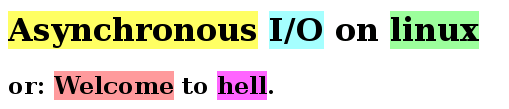
\includegraphics[width=.7\textwidth]{images/aio-linux.png}}\\
{\scriptsize (mirrored at \url{compgeom.com/~piyush/teach/4531_06/project/hell.html})}
   \\[2em]

   ``Asynchronous I/O, for example, is often infuriating.''\\
\hfill --- Robert Love. {\em Linux System Programming, 2nd ed, } page 215.

\end{center}

To motivate the need for non-blocking I/O, consider some standard I/O code:

\begin{lstlisting}[language=C]
    fd = open(...);
    read(...);
    close(fd);
\end{lstlisting}

This isn't very performant. The problem is that the {\tt read} call will
{\em block}. So, your program doesn't get to use the zillions of CPU cycles that
are happening while the I/O operation is occurring.

\paragraph{As seen previously: threads.} That can be fine if
you have some other code running to do work---for instance, other threads
do a good job mitigating the I/O latency, perhaps doing I/O themselves.
But maybe you would rather not use threads. Why not?

\begin{itemize}
\item potential race conditions;
\item overhead due to per-thread stacks; or
\item limitations due to maximum numbers of threads.
\end{itemize}

\paragraph{Non-blocking I/O.} The main point of this lecture, though,
is non-blocking/asynchronous I/O. The simplest example:

\begin{lstlisting}[language=C]
    fd = open(..., O_NONBLOCK);
    read(...); // returns instantly!
    close(fd);
\end{lstlisting}

In principle, the {\tt read} call is supposed to return instantly,
whether or not results are ready. That was easy!

Well, not so much. The {\tt O\_NONBLOCK} flag actually only has the
desired behaviour on sockets. The semantics of {\tt O\_NONBLOCK} is
for I/O calls to not block, in the sense that they should never wait
for data while there is no data available.

Unfortunately, files always have data available. Under Linux, you'd have
to use {\tt aio} calls to be able to send requests to the I/O subsystem
asynchronously and not, for instance, wait for the disk to spin up.
We won't talk about them, but they operate along the same lines as what
we will see. They just have a different API.

\paragraph{Conceptual view: non-blocking I/O.} Fundamentally,
there are two ways to find out whether I/O is ready to be queried:
polling (under UNIX, implemented via {\tt select}, {\tt poll},
and {\tt epoll}) and interrupts (under UNIX, signals).


We will describe {\tt epoll}. It is the most modern and
flexible interface. If you want to learn about \texttt{select} and \texttt{poll} at a lower level: \url{https://github.com/jzarnett/ece252/blob/master/lectures/L29-Asynchronous_I_O_with_select_poll.pdf }

The key idea is to give {\tt epoll} a bunch of file descriptors and
wait for events to happen. In particular:
     \begin{itemize}
       \item create an epoll instance ({\tt epoll\_create1});
       \item populate it with file descriptors ({\tt epoll\_ctl}); and
       \item wait for events ({\tt epoll\_wait}).
     \end{itemize}
Let's run through these steps in order.

\paragraph{Creating an {\tt epoll} instance.} Just use the API:
    \begin{lstlisting}[language=C]
   int epfd = epoll_create1(0);
    \end{lstlisting}

The return value {\tt epfd} is typed like a UNIX file
descriptor---{\tt int}---but doesn't represent any files; instead, use
it as an identifier, to talk to {\tt epoll}.

The parameter ``{\tt 0}'' represents the flags, but the only available flag
is {\tt EPOLL\_CLOEXEC}. Not interesting to you.

\paragraph{Populating the {\tt epoll} instance.} Next, you'll want
{\tt epfd} to do something. The obvious thing is to add some {\tt fd}
to the set of descriptors watched by {\tt epfd}:
    \begin{lstlisting}[language=C]
   struct epoll_event event;
   int ret;
   event.data.fd = fd;
   event.events = EPOLLIN | EPOLLOUT;
   ret = epoll_ctl(epfd, EPOLL_CTL_ADD, fd, &event);
    \end{lstlisting}

You can also use {\tt epoll\_ctl} to modify and delete descriptors from {\tt epfd}; read the manpage to find out how.

\paragraph{Waiting on an {\tt epoll} instance.} Having completed
the setup, we're ready to wait for events on any file descriptor in {\tt epfd}.
    \begin{lstlisting}[language=C]
  #define MAX_EVENTS 64

  struct epoll_event events[MAX_EVENTS];
  int nr_events;

  nr_events = epoll_wait(epfd, events, MAX_EVENTS, -1);
    \end{lstlisting}

The given {\tt -1} parameter means to wait potentially forever;
otherwise, the parameter indicates the number of milliseconds to wait.
(It is therefore ``easy'' to sleep for some number of milliseconds by
starting an {\tt epfd} and using {\tt epoll\_wait}; takes two function
calls instead of one, but allows sub-second latency.)

Upon return from {\tt epoll\_wait}, we know that we have {\tt
  nr\_events} events ready.

\subsection*{Level-Triggered and Edge-Triggered Events}
One relevant concept for these polling APIs is the concept of
\emph{level-triggered} versus \emph{edge-triggered}.  The default {\tt
  epoll} behaviour is level-triggered: it returns whenever data is
ready. One can also specify (via {\tt epoll\_ctl}) edge-triggered
behaviour: return whenever there is a change in readiness.

%\paragraph{Another Live Demo.} Now let's run some code (socket.c) that creates a
%server and reads from it, in either level-triggered mode or edge-triggered mode.

One would think that level-triggered mode would return from {\tt read}
whenever data was available, while edge-triggered mode would return
from {\tt read} whenever new data came in. Level-triggered does behave
as one would guess: if there is data available, {\tt read()} returns
the data. However, edge-triggered mode returns whenever the
state-of-readiness of the socket changes (from no-data-available to
data-available). Play with it and get a sense for how it works.

Good question to think about: when is it appropriate to choose one or the other?

\subsection*{Asynchronous I/O}
As mentioned above, the POSIX standard defines {\tt aio} calls.
Unlike just giving the {\tt O\_NONBLOCK} flag, using {\tt aio} works
for disk as well as sockets.

\paragraph{Key idea.} You specify the action to occur when I/O is ready:
    \begin{itemize}
      \item nothing;
      \item start a new thread; or
      \item raise a signal.
    \end{itemize}

Your code submits the requests using e.g. {\tt aio\_read} and {\tt aio\_write}.
If needed, wait for I/O to happen using {\tt aio\_suspend}.

\section*{Using cURL Asynchronously}
We've already seen that network communication is a great example of a way that you could use asynchronous  I/O. You can start a network request and move on to creating more without waiting for the results of the first one. For requests to different recipients, it certainly makes sense to do this.

The cURL multi interface has a lot of similarities with the regular cURL interface. Here's a simple example from \url{https://curl.haxx.se/libcurl/c/https.html} (i.e., the official docs):

\begin{lstlisting}[language=C]
#include <stdio.h>
#include <curl/curl.h>
 
int main( int argc, char** argv ) {
  CURL *curl;
  CURLcode res;
 
  curl_global_init(CURL_GLOBAL_DEFAULT);
 
  curl = curl_easy_init();
  if( curl ) {
    curl_easy_setopt(curl, CURLOPT_URL, "https://example.com/" );
    res = curl_easy_perform( curl );
    
  if( res != CURLE_OK ) {
      fprintf(stderr, "curl_easy_perform() failed: %s\n", curl_easy_strerror(res));
    }
    curl_easy_cleanup(curl);
  }
 
  curl_global_cleanup();
  return 0;
}
\end{lstlisting}

In the previous example, the call to \texttt{curl\_easy\_perform()} is blocking and we wait for the curl execution to take place. We want to change that! The tool for this is the ``multi handle'' - this is a structure that lets us have more than one curl easy handle. And rather than waiting, we can start them and then check on their progress. 

There are still the global initialization and cleanup functions. The structure for the new multi-handle type is \texttt{CURLM} (instead of \texttt{CURL}) and it is initialized with the \texttt{curl\_multi\_init()} function. 

Once we have a multi handle, we can add easy handles -- however many we need -- to the multi handle. Creation of the easy handle is the same as it is when being used alone - use \texttt{curl\_easy\_init()} to create it and then we can set however many options on this we need. Then, we add the easy handle to the multi handle with \texttt{curl\_multi\_add\_handle( CURLM* cm, CURL* eh )}.

Once we have finished putting all the easy handles into the multi handle, we can dispatch them all at once with \texttt{curl\_multi\_perform( CURLM* cm, int* still\_running )}. The second parameter is a pointer to an integer that is updated with the number of the easy handles in that multi handle that are still running. If it's down to 0, then we know that they are all done. If it's nonzero it means that some of them are still in progress.

This does mean that we're going to call\texttt{curl\_multi\_perform()} more than once. Doing so doesn't restart or interfere with anything that was already in progress -- it just gives us an update on the status of what's going on. We can check as often as we'd like, but the intention is of course to do something useful while the asynchronous I/O request(s) are going on. Otherwise, why not make it synchronous?

Suppose we've run out of things to do though. What then? Well, we can wait, if we want, using \texttt{curl\_multi\_wait( CURLM *multi\_handle, struct curl\_waitfd extra\_fds[], unsigned int extra\_nfds, int timeout\_ms, int *numfds )} . This function will block the current thread until something happens (some event occurs).

The first parameter is the multi handle, which makes sense. The second parameter is a structure of extra file descriptors you can wait on (but we will always want this to be NULL in this course) and the third parameter is the count (the size of the provided array) which would also be zero here. Then the second-last parameter is a maximum time to wait. The last parameter is a pointer that will be updated with the actual number of ``interesting'' events that occurred (interesting is the word used in the specifications, and what it means is mysterious). For a simple use case you can ignore most of the parameters and just wait for something to happen and go from there.

In the meantime though, the perform operations are happening, and so are whatever callbacks we have set up (if any). And as the I/O operation moves through its life cycle, the state of the easy handle is updated appropriately. Each easy handle has an associated status message as well as a return code.

Why both? Well - one is about what the status of the request is. The message could be, for example ``done'', but does that mean finished with success or finished with an error? For the second one tells us about that. We can ask about the status of the request using \texttt{curl\_multi\_info\_read( CURLM* cm, int* msgs\_left )}. This returns a pointer to information ``next'' easy handle, if there is one. The return value is a pointer to a struct of type \texttt{CURLMsg}. Along side this, the parameter \texttt{msgs\_left} is updated to say how many messages remain (so you don't have to remember or know in advance, really). 

We will therefore check the \texttt{CURLMsg} message to see what happened and make sure all is well. If our message that we got back with the info read is called \texttt{m}, What we are looking for is that the \texttt{m->msg} is equal to \texttt{CURLMSG\_DONE} -- request completed. If not, this request is still in progress and we aren't ready to evaluate whether it was successful or not. If there are more handles to look at, we should go on to the next. If it is done, we should look at the return code in and the result, in \texttt{m->data.result}. If it is \texttt{CURLE\_OK} then everything succeeded. If it's anything else, it indicates an error.

When a handle has finished, you need to remove it from the multi handle. A pointer to it is inside the \texttt{CURLMsg} under \texttt{m->easy\_handle}. It is removed with \texttt{curl\_multi\_remove\_handle( CURLM* cm, CURL eh )}. Once removed, it should be cleaned up like normal with \texttt{curl\_easy\_cleanup( CURL* eh )}.

There is of course the corresponding cleanup function \texttt{curl\_multi\_cleanup( CURLM * cm ) } for the multi handle when we are done with all the easy handles inside. The last step, as before, is to use the global cleanup function. After that we are done. 

Let's consider the following code example by Clemens Gruber~\cite{curlmulti}, with slight modifications for compactness, formatting, and to remember the cleanup. This example puts together all the things we talked about in one compact code segment. Here, the callback does nothing, but that's okay -- it's just to show what you could do with it.

\begin{lstlisting}[language=C]
#include <stdio.h>
#include <stdlib.h>
#include <unistd.h>
#include <curl/multi.h>

#define MAX_WAIT_MSECS 30*1000 /* Wait max. 30 seconds */

const char *urls[] = {
  "http://www.microsoft.com",
  "http://www.yahoo.com",
  "http://www.wikipedia.org",
  "http://slashdot.org"
};
#define CNT 4

size_t cb(char *d, size_t n, size_t l, void *p) {
  /* take care of the data here, ignored in this example */
  return n*l;
}

void init( CURLM *cm, int i ) {
  CURL *eh = curl_easy_init();
  curl_easy_setopt( eh, CURLOPT_WRITEFUNCTION, cb );
  curl_easy_setopt( eh, CURLOPT_HEADER, 0L );
  curl_easy_setopt( eh, CURLOPT_URL, urls[i] );
  curl_easy_setopt( eh, CURLOPT_PRIVATE, urls[i]) ;
  curl_easy_setopt( eh, CURLOPT_VERBOSE, 0L );
  curl_multi_add_handle( cm, eh );
}

int main( int argc, char** argv ) {
    CURLM *cm = NULL;
    CURL *eh = NULL;
    CURLMsg *msg = NULL;
    CURLcode return_code = 0;
    int still_running = 0; 
    int msgs_left = 0;
    int http_status_code;
    const char *szUrl;

    curl_global_init( CURL_GLOBAL_ALL );
    cm = curl_multi_init( );

    for ( int i = 0; i < CNT; ++i ) {
        init( cm, i );
    }

    curl_multi_perform( cm, &still_running );

    do {
        int numfds = 0;
        int res = curl_multi_wait( cm, NULL, 0, MAX_WAIT_MSECS, &numfds );
        if( res != CURLM_OK ) {
            fprintf( stderr, "error: curl_multi_wait() returned %d\n", res );
            return EXIT_FAILURE;
        }
        curl_multi_perform( cm, &still_running );

    } while( still_running );

    while ( ( msg = curl_multi_info_read( cm, &msgs_left ) ) ) {
        if ( msg->msg == CURLMSG_DONE ) {
            eh = msg->easy_handle;

            return_code = msg->data.result;
            if ( return_code != CURLE_OK ) {
                fprintf( stderr, "CURL error code: %d\n", msg->data.result );
                continue;
            }

            // Get HTTP status code
            http_status_code = 0;
            szUrl = NULL;

            curl_easy_getinfo( eh, CURLINFO_RESPONSE_CODE, &http_status_code );
            curl_easy_getinfo( eh, CURLINFO_PRIVATE, &szUrl );

            if( http_status_code == 200 ) {
                printf( "200 OK for %s\n", szUrl ) ;
            } else {
                fprintf( stderr, "GET of %s returned http status code %d\n", szUrl, http_status_code );
            }

            curl_multi_remove_handle( cm, eh );
            curl_easy_cleanup( eh );
        } else {
            fprintf( stderr, "error: after curl_multi_info_read(), CURLMsg=%d\n", msg->msg );
        }
    }
    curl_multi_cleanup( cm );
    curl_global_cleanup();
    return 0;
}
\end{lstlisting}

You may wonder about re-using an easy handle rather than removing and destroying it and making a new one. The official docs say that you can re-use one, but you have to remove it from the multi handle and then re-add it, presumably after having changed anything that you want to change about that handle. 

In this example all requests had the same (useless) callback, but of course you could have different callbacks for different easy handles if you wanted them to do different things. 


\section*{Building Servers: Concurrent Socket I/O}

\paragraph{Your Choices.} The first two both use blocking I/O, while the second two use
non-blocking I/O~~\cite{gplus:concurrent}:
    \begin{itemize}
      \item Blocking I/O; 1 process per request.
      \item Blocking I/O; 1 thread per request.
      \item Asynchronous I/O, pool of threads, callbacks, each thread handles multiple connections.
      \item Nonblocking I/O, pool of threads, multiplexed with select/poll,
        event-driven, each thread handles multiple connections.
    \end{itemize}

\paragraph{Blocking I/O; 1 process per request.}
This is the old Apache model.
  \begin{itemize}
    \item The main thread waits for connections.
    \item Upon connect, the main thread forks off a new process, which completely
      handles the connection.
    \item Each I/O request is blocking, e.g., reads wait until more data arrives.
  \end{itemize}

Advantage: 
  \begin{itemize}
    \item ``Simple to undertand and easy to program.''
  \end{itemize}

Disadvantage:
  \begin{itemize}
    \item High overhead from starting 1000s of processes.
      (We can somewhat mitigate this using process pools).
  \end{itemize}
This method can handle $\sim$10 000 processes, but doesn't generally scale beyond that, and
uses many more resources than the alternatives.

\paragraph{Blocking I/O; 1 thread per request.}
    We know that threads are more lightweight than processes. So let's use threads instead
of processes. Otherwise, this is the same as 1 process per request, but with less overhead.
I/O is the same---it is still blocking.

    Advantage:
    \begin{itemize}
      \item Still simple to understand and easy to program.
    \end{itemize}

    Disadvantages:
    \begin{itemize}
      \item Overhead still piles up, although less than processes.
      \item New complication: race conditions on shared data.
    \end{itemize}

\paragraph{Asynchronous I/O.} The other two choices don't assign one thread or process per connection,
but instead multiplex the threads to connections. We'll first talk
about using asynchronous I/O with select or poll.  

Here are (from 2006) some performance benefits of using asynchronous
I/O on lighttpd~\cite{lttpd}.

    \begin{tabular}{llrrr}
    version & & fetches/sec & bytes/sec & CPU idle \\
    1.4.13 & sendfile & 36.45 & 3.73e+06 & 16.43\% \\
    1.5.0 & sendfile & 40.51 & 4.14e+06 & 12.77\% \\
    1.5.0 & linux-aio-sendfile & 72.70 & 7.44e+06 & 46.11\% \\
    \end{tabular}

(Workload: $2\times 7200$ RPM in RAID1, 1GB RAM, transferring 10GBytes on a 100MBit network).

The basic workflow is as follows: 
   \begin{enumerate}
     \item enqueue a request;
     \item \ldots ~do something else;
     \item (if needed) periodically check whether request is done; and
     \item read the return value.
   \end{enumerate}

Some code which uses the Linux asynchronous I/O model is:
\begin{lstlisting}[language=C]
#include <aio.h>

int main() {
    // so far, just like normal
    int file = open("blah.txt", O_RDONLY, 0);

    // create buffer and control block
    char* buffer = new char[SIZE_TO_READ];
    aiocb cb;
    
    memset(&cb, 0, sizeof(aiocb));
    cb.aio_nbytes = SIZE_TO_READ;
    cb.aio_fildes = file;
    cb.aio_offset = 0;
    cb.aio_buf = buffer;

    // enqueue the read
    if (aio_read(&cb) == -1) { /* error handling */ }

    do {
      // ... do something else ...
    while (aio_error(&cb) == EINPROGRESS); // poll

    // inspect the return value
    int numBytes = aio_return(&cb);
    if (numBytes == -1) { /* error handling */ }

    // clean up
    delete[] buffer;
    close(file);
\end{lstlisting}

\paragraph{Using Select/Poll.} The idea is to improve performance
by letting each thread handle multiple connections.
When a thread is ready, it uses select/poll to find work:
    \begin{itemize}
      \item perhaps it needs to read from disk into a mmap'd tempfile;
      \item perhaps it needs to copy the tempfile to the network.
    \end{itemize}

In either case, the thread does work and updates the request state.









\chapter*{9 --- Of Asgard \& Hel}

\addcontentsline{toc}{chapter}{9 --- Of Asgard \& Hel}

\section*{Norse Mythology}
Everything came into creation in the gap between fire and ice, and the World Tree (Yggdrasil) connects the nine worlds. Asgard is the home of the \AE sir, the Norse gods. Helheim, or simply Hel, is the underworld where the dead go upon their death. In Hel or Asgard (it's not entirely clear), there is Valhalla, hall of the honoured dead. Those who die in battle and are judged worthy will be carried to Valhalla by the Valkyries. There they will reside until they are called upon to aid in Odin's fight with the wolf Fenrir in Ragnar\"ok\footnote{German: G\"otterd\"ammerung - ``Twilight of the gods''}, the doom of the gods\footnote{Spoiler alert: this isn't going to end well for Odin.}. For the curious, humans live in the ``middle realm'', Midg\aa rd, surrounded by the serpent Jormungand, who will fight against Thor in  Ragnar\"ok. Thor will kill the serpent, but the serpent's poison will also finish off Thor\footnote{Sorry if I've just spoiled the plot of a Marvel movie.}.

Aside from my obvious passion about the subject, why are we talking about Norse Mythology? We're going to examine some very useful tools for programming called Valgrind and Helgrind (also Cachegrind). Note that the -grind endings on those are pronounced like ``grinned''. Where do they take their names from? Valgrind is the gateway to Valhalla; a gate that only the worthy can pass. Helgrind is the gateway to, well, Hel. Which despite being the source of the English word ``Hell'', is not the place where sinners go. It's just the place where the dead go. Sadly, the authors of Cachegrind failed to choose a name that corresponds to a location in the nine worlds of Norse mythology. There are eight unused realms. They really could have.

But all of these, in program form, are analysis tools for your (usually) C and C++ programs. They are absolute murder on performance, but they are wonderful for finding errors in your program. To use them you will start the tool of your choice and instruct it to invoke your program. The target program then runs under the ``supervision'' of the tool. This results in running dramatically slower than normal, but you get additional checks and monitoring of the program. It's important to enable debugging symbols in your compile (\texttt{-g} option if using \texttt{gcc}) if you want stack traces to be useful.

Let's start with a quick summary of each of the tools from~\cite{valgrind:tools}, followed by a more detailed explanation.

\subsection*{Valgrind (or Memcheck) }
Valgrind is the base name of the project and by default what it's going to do is run the memcheck tool. The purpose of memcheck is to look into all memory reads, writes, and to intercept and analyze every call to \texttt{malloc}/\texttt{free} and \texttt{new}/\texttt{delete}. Thus, memcheck will check all memory accesses and allocations/deallocations, and can find problems like:
\begin{itemize}
	\item Accessing uninitialized memory
	\item Reading off the end of an array
	\item Memory leaks (failing to free allocated memory)
	\item Incorrect freeing of memory (double free calls or a mismatch)
	\item Incorrect use of C standard functions like \texttt{memcpy}
	\item Using memory after it's been freed.
	\item Asking for an invalid number of bytes in an allocation (negative\textinterrobang)
\end{itemize}

These errors will be reported to the console when they occur. Ideally, this will help you find the source of the problem. 

I decided to run Valgrind with memcheck against the solution I wrote to the ECE~254 S15 exam question for searching an array using pthreads. I am happy to report that memcheck reports that the official solution has no memory leaks. If you do things right, you get something that looks like the example below. 
\begin{verbatim}
jz@Loki:~/ece254$ valgrind ./search
==8476== Memcheck, a memory error detector
==8476== Copyright (C) 2002-2013, and GNU GPL'd, by Julian Seward et al.
==8476== Using Valgrind-3.10.0.SVN and LibVEX; rerun with -h for copyright info
==8476== Command: /usr/local/bin/search
==8476== 
usage: search [arguments] [options]
arguments:
         for text
         in directory
options:
         -c | --case-sensitive
         -s | --show-filenames-only
==8476== 
==8476== HEAP SUMMARY:
==8476==     in use at exit: 0 bytes in 0 blocks
==8476==   total heap usage: 0 allocs, 0 frees, 0 bytes allocated
==8476== 
==8476== All heap blocks were freed -- no leaks are possible
==8476== 
==8476== For counts of detected and suppressed errors, rerun with: -v
==8476== ERROR SUMMARY: 0 errors from 0 contexts (suppressed: 0 from 0)
\end{verbatim}

Okay, everything going perfectly is unlikely in anything other than a small program. The exam question I used this on is something like 62 lines (including blanks). So it's a trivial program. But I'll sabotage it a bit so we get a more interesting result. Suppose I delete from the code two of the \texttt{free()} calls.

\begin{verbatim}
jz@Loki:~/ece254$ valgrind ./search 
==8678== Memcheck, a memory error detector
==8678== Copyright (C) 2002-2013, and GNU GPL'd, by Julian Seward et al.
==8678== Using Valgrind-3.10.0.SVN and LibVEX; rerun with -h for copyright info
==8678== Command: ./search
==8678== 
Found at 11 by thread 1 
Found at 22 by thread 3 
==8678== 
==8678== HEAP SUMMARY:
==8678==     in use at exit: 1,614 bytes in 4 blocks
==8678==   total heap usage: 17 allocs, 13 frees, 2,822 bytes allocated
==8678== 
==8678== LEAK SUMMARY:
==8678==    definitely lost: 0 bytes in 0 blocks
==8678==    indirectly lost: 0 bytes in 0 blocks
==8678==      possibly lost: 0 bytes in 0 blocks
==8678==    still reachable: 1,614 bytes in 4 blocks
==8678==         suppressed: 0 bytes in 0 blocks
==8678== Rerun with --leak-check=full to see details of leaked memory
==8678== 
==8678== For counts of detected and suppressed errors, rerun with: -v
==8678== ERROR SUMMARY: 0 errors from 0 contexts (suppressed: 0 from 0)
\end{verbatim}

If you take the program's suggestion to use \verb+--leak-check=full+ then you end up with a bit more detail about where you made the mistake. Of course, it's important to know where to look; in the example below, lines 49 and 24 in the file \texttt{search.c} are the locations of the \texttt{malloc} calls that lack a matching call to \texttt{free}. It can't tell you where the call to \texttt{free} should go, only where the memory that isn't freed was allocated.

\begin{verbatim}
==8553== 16 bytes in 4 blocks are definitely lost in loss record 1 of 2
==8553==    at 0x4C2AB80: malloc (in /usr/lib/valgrind/vgpreload_memcheck-amd64-linux.so)
==8553==    by 0x40084D: search (search.c:49)
==8553==    by 0x4E3F181: start_thread (pthread_create.c:312)
==8553==    by 0x514F47C: clone (clone.S:111)
==8553== 
==8553== 48 bytes in 4 blocks are definitely lost in loss record 2 of 2
==8553==    at 0x4C2AB80: malloc (in /usr/lib/valgrind/vgpreload_memcheck-amd64-linux.so)
==8553==    by 0x40074E: main (search.c:24)

\end{verbatim}

But it's also important to learn what to ignore (or what's out of our hands). I decided to deploy Valgrind on the solution to the producer-consumer problem from ECE~254 and I ended up with a result that says:

\begin{verbatim}
==8734==      possibly lost: 544 bytes in 2 blocks
\end{verbatim}

Hmm. Let's dig into that with the \verb+--leak-check=full+ option:

\begin{verbatim}
==8734== 272 bytes in 1 blocks are possibly lost in loss record 1 of 2
==8734==    at 0x4C2CC70: calloc (in /usr/lib/valgrind/vgpreload_memcheck-amd64-linux.so)
==8734==    by 0x4012E54: _dl_allocate_tls (dl-tls.c:296)
==8734==    by 0x4E3FDA0: pthread_create@@GLIBC_2.2.5 (allocatestack.c:589)
==8734==    by 0x400A57: main (mutex.c:64)
\end{verbatim}

Looking in the file, at that line, we see a call to \texttt{pthread\_create} and this is therefore probably nothing we need to do anything about. Or is it? In-class example will tell...

From the Valgrind FAQ, how to read the leak summary:
\begin{itemize}
	\item \textbf{Definitely lost}: a clear memory leak. Fix it.
	\item \textbf{Indirectly lost}: a problem with a pointer based structure (e.g., you've lost the head of the linked list, but the rest of the list is indirectly lost.) Generally, fixing the definitely lost items should be enough to clear up the indirectly lost stuff.
	\item \textbf{Possibly lost}: the program is leaking memory unless weird things are going on with pointers where you're pointing them to the middle of an allocated block.
	\item \textbf{Still reachable}: this is memory that was still allocated that might otherwise have been freed, but references to it exist so it at least wasn't lost.
	\item \textbf{Suppressed}: you can configure the tool to ignore things and those will appear in the suppressed category.
\end{itemize}



\subsection*{Helgrind}  
The purpose of Helgrind is to detect errors in the use of POSIX pthreads. In a way, Helgrind is a pretty neat tool for improving performance, even though it doesn't actually directly speed anything up. When we take a single-threaded program and split it off into a multithreaded program, we may introduce a lot of errors (or at least, introduce the possibility of a lot of errors). Truthfully, humans are not very good at parallel thinking; we are very much sequential. But a program that is fast and wrong is probably less useful than one that is slow and correct. Can we make it faster and still have it be correct? That's the goal of Helgrind: after you parallelize your code, it will do some automatic checking of the code to determine where, if anywhere, there are concurrency problems. It can't prove that your program is correct (if only) but it can at least catch some of the common problems you might introduce when writing a parallel program. Helgrind classifies errors into three basic categories:

\begin{enumerate}[noitemsep]
	\item Misuses of the pthreads API;
	\item Lock ordering problems; and
	\item Data races.
\end{enumerate}

The first category does not require much explanation. These are just some programming errors related to the pthread API calls. Some examples from~\cite{helgrind}:

\begin{itemize}[noitemsep]
	\item Unlocking a mutex that is unlocked;
	\item Deallocation of memory with a locked mutex in it; or
	\item Thread exit while holding a lock.
\end{itemize}
\ldots and many more.

A quick example of an error message from Helgrind, also from~\cite{helgrind}:

\begin{verbatim}
Thread #1 unlocked a not-locked lock at 0x7FEFFFA90
   at 0x4C2408D: pthread_mutex_unlock (hg_intercepts.c:492)
   by 0x40073A: nearly_main (tc09_bad_unlock.c:27)
   by 0x40079B: main (tc09_bad_unlock.c:50)
  Lock at 0x7FEFFFA90 was first observed
   at 0x4C25D01: pthread_mutex_init (hg_intercepts.c:326)
   by 0x40071F: nearly_main (tc09_bad_unlock.c:23)
   by 0x40079B: main (tc09_bad_unlock.c:50)
\end{verbatim}



The second category of errors should be familiar to you from your operating systems class as a source of potential deadlock.

\begin{multicols}{2}
\textbf{Thread P}\vspace{-2em}
  \begin{verbatim}
	 1. wait( a ) 
	 2. wait( b )
	 3. [critical section]
	 4. signal( a )
	 5. signal( b )
  \end{verbatim}
\columnbreak
\textbf{Thread Q}\vspace{-2em}
  \begin{verbatim}
	 1. wait( b ) 
	 2. wait( a )
	 3. [critical section]
	 4. signal( b )
	 5. signal( a )
  \end{verbatim}
\end{multicols}
\vspace{-2em}

In this case, if the interleaving of these happens to work out in a couple of particular ways, then we get deadlock because thread P holds mutex \texttt{a} and thread Q holds mutex \texttt{b} and each waits for the mutex that the other one has. The example is slightly silly, of course, because it's super easy to see; in normal code they would probably be separated by some number of lines, and the mutexes will probably not be called \texttt{a} and \texttt{b} (isn't using meaningful variable names one of those things you were supposed to learn to do in introductory programming\textinterrobang) and there therefore will not necessarily be an obvious (alphabetical) order.

Helgrind builds a directed graph of lock acquisitions. When a thread acquires a lock, Helgrind checks to see whether a cycle exists. If so, then there is potential for a deadlock~\cite{helgrind}. Helgrind will report as an error the initial order (the first order seen is the one viewed as ``correct'') and the ``incorrect'' order that is the source of the potential problem. Really, though, all that matters is consistency---following the same order. You may change either of the acquisition orders to match the other. See the example below~\cite{helgrind}:

\begin{verbatim}
Thread #1: lock order "0x7FF0006D0 before 0x7FF0006A0" violated

Observed (incorrect) order is: acquisition of lock at 0x7FF0006A0
   at 0x4C2BC62: pthread_mutex_lock (hg_intercepts.c:494)
   by 0x400825: main (tc13_laog1.c:23)

 followed by a later acquisition of lock at 0x7FF0006D0
   at 0x4C2BC62: pthread_mutex_lock (hg_intercepts.c:494)
   by 0x400853: main (tc13_laog1.c:24)

Required order was established by acquisition of lock at 0x7FF0006D0
   at 0x4C2BC62: pthread_mutex_lock (hg_intercepts.c:494)
   by 0x40076D: main (tc13_laog1.c:17)

 followed by a later acquisition of lock at 0x7FF0006A0
   at 0x4C2BC62: pthread_mutex_lock (hg_intercepts.c:494)
   by 0x40079B: main (tc13_laog1.c:18)
\end{verbatim}

The third category we have discussed already. Recall the earlier definition of a race condition. This is a difficult problem to find sometimes; what Helgrind will do is examine where multiple threads are accessing shared memory without the use of locks. Let's cut to the chase and see it in action:


\begin{verbatim}
jz@Loki:~/ece459$ valgrind --tool=helgrind ./datarace
==10389== Helgrind, a thread error detector
==10389== Copyright (C) 2007-2013, and GNU GPL'd, by OpenWorks LLP et al.
==10389== Using Valgrind-3.10.0.SVN and LibVEX; rerun with -h for copyright info
==10389== Command: ./datarace
==10389== 
==10389== ---Thread-Announcement------------------------------------------
==10389== 
==10389== Thread #1 is the program's root thread
==10389== 
==10389== ---Thread-Announcement------------------------------------------
==10389== 
==10389== Thread #2 was created
==10389==    at 0x515543E: clone (clone.S:74)
==10389==    by 0x4E44199: do_clone.constprop.3 (createthread.c:75)
==10389==    by 0x4E458BA: pthread_create@@GLIBC_2.2.5 (createthread.c:245)
==10389==    by 0x4C30C90: ??? (in /usr/lib/valgrind/vgpreload_helgrind-amd64-linux.so)
==10389==    by 0x40068D: main (datarace.c:12)
==10389== 
==10389== ----------------------------------------------------------------
==10389== 
==10389== Possible data race during read of size 4 at 0x60104C by thread #1
==10389== Locks held: none
==10389==    at 0x40068E: main (datarace.c:13)
==10389== 
==10389== This conflicts with a previous write of size 4 by thread #2
==10389== Locks held: none
==10389==    at 0x40065E: child_fn (datarace.c:6)
==10389==    by 0x4C30E26: ??? (in /usr/lib/valgrind/vgpreload_helgrind-amd64-linux.so)
==10389==    by 0x4E45181: start_thread (pthread_create.c:312)
==10389==    by 0x515547C: clone (clone.S:111)
==10389== 
==10389== ----------------------------------------------------------------
==10389== 
==10389== Possible data race during write of size 4 at 0x60104C by thread #1
==10389== Locks held: none
==10389==    at 0x400697: main (datarace.c:13)
==10389== 
==10389== This conflicts with a previous write of size 4 by thread #2
==10389== Locks held: none
==10389==    at 0x40065E: child_fn (datarace.c:6)
==10389==    by 0x4C30E26: ??? (in /usr/lib/valgrind/vgpreload_helgrind-amd64-linux.so)
==10389==    by 0x4E45181: start_thread (pthread_create.c:312)
==10389==    by 0x515547C: clone (clone.S:111)
==10389== 
==10389== 
==10389== For counts of detected and suppressed errors, rerun with: -v
==10389== Use --history-level=approx or =none to gain increased speed, at
==10389== the cost of reduced accuracy of conflicting-access information
==10389== ERROR SUMMARY: 2 errors from 2 contexts (suppressed: 0 from 0)
\end{verbatim}

Note that we get two stack traces here: we have a read after write, and a write after write. Why? Because the operation in question is \texttt{var++} which necessitates fetching the current value of \texttt{var} (reading it) and incrementing it (then writing it back).

How does Helgrind work? It examines the use of the standard threading primitives---lock, unlock, signal/post, wait, etc. Anything that implies there might be an ordering between events is taken and added to a directed acyclic graph that represents these dependencies. If memory is accessed from two different threads and there is no path through this directed acyclic graph that indicates an ordering, then Helgrind reports a race~\cite{helgrind}. Obviously, at least one of these accesses must be a write. (Recall: there is no read after read dependency).

Also cool: you can ask Helgrind to try to tell you about variable names (if it can) with the command line option \texttt{--read-var-info=yes}. Then it will tell you something interesting like:

\begin{verbatim}
==10454== Location 0x60104c is 0 bytes inside global var "var"
==10454== declared at datarace.c:3
\end{verbatim}

These will give you indications of where you need to introduce synchronization of some kind (semaphore, mutex, condition variable, etc). The authors of Helgrind assume that if it tells you where the problem is, you will figure out what variables are affected and how to properly prevent data races. You might find this frustrating, in the sense of a serial complainer who thinks that he or she can just moan about what's wrong without bringing forward any suggestions about how to fix the problems. 

A note about Helgrind for later, since we're going to dive into OpenMP. Helgrind + OpenMP + Linux can cause the occasional problem in GCC 4.2 and 4.3 (perhaps fixed in GCC 4.6.3\footnote{\url{http://valgrind-users.narkive.com/QARaSvBN/helgrind-and-openmp-on-gcc}}). But the ``futex'' system call in Linux is not visible to Helgrind so it won't figure things out. If you have old GCC, you can rebuild it with the option \texttt{--disable-linux-futex} and it won't generate ``futex'' syscalls.

\subsection*{Cachegrind}

Cachegrind is another tool in the package and this one is much more performance oriented than the other two tools. Yes, Valgrind's memcheck and Helgrind look for errors in your program that are likely to lead to slowdowns (memory leaks) or make it easier to parallelize (spawn threads) without introducing errors. Cachegrind, however, does a simulation of how your program interacts with cache and evaluates how your program does on branch prediction. As we discussed earlier, cache misses and branch mispredicts have a huge impact on performance.

Recall that a miss from the fastest cache results in a small penalty (perhaps, 10 cycles); a miss that requires going to memory requires about 200 cycles. A mispredicted branch costs somewhere between 10-30 cycles. All figures \& estimates from the cachegrind manual~\cite{cachegrind}.

Cachegrind reports data about:
\begin{itemize}
	\item The First Level Instruction Cache (I1) [L1 Instruction Cache]
	\item The First Level Data Cache (D1) [L1 Data Cache]
	\item The Last Level Cache (LL) [L3 Cache].
\end{itemize}

Unlike for normal Valgrind operation, you probably want to turn optimizations on (\texttt{-O2} or perhaps \texttt{-O3} in \texttt{gcc}). You still want debugging symbols, of course, but enabling optimizations will tell you more about what is going to happen in the released version of your program.

If I instruct cachegrind to run on the search example (same one from above), using the \texttt{--branch-sim=yes} option because by default it won't show it:

\begin{verbatim}
jz@Loki:~/ece254$ valgrind --tool=cachegrind --branch-sim=yes ./search
==16559== Cachegrind, a cache and branch-prediction profiler
==16559== Copyright (C) 2002-2013, and GNU GPL'd, by Nicholas Nethercote et al.
==16559== Using Valgrind-3.10.0.SVN and LibVEX; rerun with -h for copyright info
==16559== Command: ./search
==16559== 
--16559-- warning: L3 cache found, using its data for the LL simulation.
Found at 11 by thread 1 
Found at 22 by thread 3 
==16559== 
==16559== I   refs:      310,670
==16559== I1  misses:      1,700
==16559== LLi misses:      1,292
==16559== I1  miss rate:    0.54%
==16559== LLi miss rate:    0.41%
==16559== 
==16559== D   refs:      114,078  (77,789 rd   + 36,289 wr)
==16559== D1  misses:      4,398  ( 3,360 rd   +  1,038 wr)
==16559== LLd misses:      3,252  ( 2,337 rd   +    915 wr)
==16559== D1  miss rate:     3.8% (   4.3%     +    2.8%  )
==16559== LLd miss rate:     2.8% (   3.0%     +    2.5%  )
==16559== 
==16559== LL refs:         6,098  ( 5,060 rd   +  1,038 wr)
==16559== LL misses:       4,544  ( 3,629 rd   +    915 wr)
==16559== LL miss rate:      1.0% (   0.9%     +    2.5%  )
==16559== 
==16559== Branches:       66,622  (65,097 cond +  1,525 ind)
==16559== Mispredicts:     7,202  ( 6,699 cond +    503 ind)
==16559== Mispred rate:     10.8% (  10.2%     +   32.9%   )

\end{verbatim}

So we see a breakdown of the instruction accesses, data accesses, and how well the last level of cache (L3 here) does. 

Why did I say enable optimization? Well, here's the output of the search program if I compile with the \texttt{-O2} option:

\begin{verbatim}
jz@Loki:~/ece254$ valgrind --tool=cachegrind --branch-sim=yes ./search
==16618== Cachegrind, a cache and branch-prediction profiler
==16618== Copyright (C) 2002-2013, and GNU GPL'd, by Nicholas Nethercote et al.
==16618== Using Valgrind-3.10.0.SVN and LibVEX; rerun with -h for copyright info
==16618== Command: ./search
==16618== 
--16618-- warning: L3 cache found, using its data for the LL simulation.
Found at 11 by thread 1 
Found at 22 by thread 3 
==16618== 
==16618== I   refs:      306,169
==16618== I1  misses:      1,652
==16618== LLi misses:      1,286
==16618== I1  miss rate:    0.53%
==16618== LLi miss rate:    0.42%
==16618== 
==16618== D   refs:      112,015  (76,522 rd   + 35,493 wr)
==16618== D1  misses:      4,328  ( 3,353 rd   +    975 wr)
==16618== LLd misses:      3,201  ( 2,337 rd   +    864 wr)
==16618== D1  miss rate:     3.8% (   4.3%     +    2.7%  )
==16618== LLd miss rate:     2.8% (   3.0%     +    2.4%  )
==16618== 
==16618== LL refs:         5,980  ( 5,005 rd   +    975 wr)
==16618== LL misses:       4,487  ( 3,623 rd   +    864 wr)
==16618== LL miss rate:      1.0% (   0.9%     +    2.4%  )
==16618== 
==16618== Branches:       65,827  (64,352 cond +  1,475 ind)
==16618== Mispredicts:     7,109  ( 6,596 cond +    513 ind)
==16618== Mispred rate:     10.7% (  10.2%     +   34.7%   )
\end{verbatim}

Interesting results: our data and instruction miss rates went down marginally but the branch mispredict rates went up! Well, sort of---there were fewer branches and thus fewer we got wrong as well as fewer we got right. So the total cycles lost to mispredicts went down. Is this an overall win for the code? Yes. 

In some cases it's not so clear cut, and we could do a small calculation. If we just take a look at the LL misses (4~544 vs 4~487) and assume they take 200 cycles, and the branch miss penalty is 200 cycles, it went from 908~800 wasted cycles to 897~400; a decrease of 11~400 cycles. Repeat for each of the measures and sum them up to determine if things got better overall and by how much. Also be sure that you're reasoning about a realistic workload.

Cachegrind also produces a more detailed output file, titled cachegrind.out.<pid> (the PID in the example is 16618). This file is not especially human-readable, but we can ask the associated tool \texttt{cg\_annotate} to break it down for us, and if we have the source code available, so much the better, because it will give you line by line information. That's way too much to show even in the notes, so it's the sort of thing I can show in class (or you can create for yourself) but here's a small excerpt from the \texttt{search.c} example:



{\scriptsize
\begin{verbatim}
--------------------------------------------------------------------------------
-- Auto-annotated source: /home/jz/ece254/search.c
--------------------------------------------------------------------------------
 Ir I1mr ILmr Dr D1mr DLmr Dw D1mw DLmw Bc Bcm Bi Bim 
127    1    1 96    3    0  4    0    0 23  11  0   0      for ( int i = arg->startIndex; i < arg->endIndex; ++i ) {
147    0    0 84    3    2  0    0    0 21   9  0   0          if ( array[i] == arg->searchValue ) {
  6    0    0  4    0    0  2    0    0  0   0  0   0              *result = i;
  2    0    0  0    0    0  0    0    0  0   0  0   0              break;
  .    .    .  .    .    .  .    .    .  .   .  .   .          }
  .    .    .  .    .    .  .    .    .  .   .  .   .      }
\end{verbatim}
}

Cachegrind is very\ldots verbose\ldots and it can be very hard to come up with useful changes based on what you see\ldots assuming your eyes don't glaze over when you see the numbers. Probably the biggest performance impact is last level cache misses (those appear as DLmr or DLmw). They have the highest penalty. You might also try to look at the Bcm and Bim (branch mispredictions) to see if you can give some better hints about what the likelihood of branch prediction is~\cite{cachegrind}. Of course, to learn more about how Cachegrind actually does what it does and how it runs the simulation, the manual is worth reading. Not that anybody reads manuals anymore\ldots Just give it a shot, when you get stuck, google the problem, click the first stack overflow link result\ldots









\chapter*{10 --- Use of Locks}

\addcontentsline{toc}{chapter}{10 --- Use of Locks}

\section*{Appropriate Use of Locking}

In previous courses you learned about locking and how it all works, then we did a quick recap of what you need to know about it. And perhaps you were given some guidance in the use of locks, but probably in earlier scenarios it was sufficient to just avoid all the bad stuff (data races, deadlock, starvation). That's important but is no longer enough. Now we need to use locking and other synchronization techniques appropriately. 

I like to say that critical sections should be as large as they need to be but no larger. That is to say, if we have some shared data that needs to be protected by some mutual exclusion constructs, we need to consider carefully where to place the statements. They should be placed such that the critical section contains all of the shared accesses, both reads \textit{and} writes, but also does contain any extraneous statements. The ones that don't need to be there are those that don't operate on shared data. 

This can mean that a block of code or contents of a function need to be re-arranged to move some statements up or down so they are no longer in the critical section. Sometimes control flow or other very short statements might get swept into the critical section being created to make sure all goes as planned but those should be the exception rather than the rule.

Let's consider a short code example from the producer-consumer problem. We have some global variables below that will be initialized as appropriate. There is also a definition of the function that will consume the data.

\begin{lstlisting}[language=C]
sem_t spaces;
sem_t items;
int counter;
int* buffer;
int pindex = 0;
int cindex = 0;
int ctotal = 0;
pthread_mutex_t prod_mutex;
pthread_mutex_t con_mutex;

void consume( int to_consume );

\end{lstlisting}

And then here is our single-threaded code for the consumer. We want our consumer threads to consume exactly {\tt MAX\_ITEMS\_CONSUMED} items and then cleanly exit; we don't want anything to stay stuck at a mutex for instance.

\begin{lstlisting}[language=C]
void* consumer( void* arg ) { 
  while( ctotal < MAX_ITEMS_CONSUMED ) {
    sem_wait( &items );
    consume( buffer[cindex] );
    buffer[cindex] = -1;
    cindex = (cindex + 1) % BUFFER_SIZE;
    ++ctotal;
    sem_post( &spaces );
  }
}
\end{lstlisting}

To this we need to add some mutual exclusion if we want to allow multiple consumers at the same time. I'll leave aside the case of only allowing one consumer by putting the lock and unlock statements outside the while loop since that defeats the purpose of having multiple threads altogether. One approach we could take is that which allows exactly one consumer to run at a time, as below. But what's wrong with this?

\begin{lstlisting}[language=C]
void* consumer( void* arg ) { 
  while( ctotal < MAX_ITEMS_CONSUMED ) {
    pthread_mutex_lock( &con_mutex );
    sem_wait( &items );
    consume( buffer[cindex] );
    buffer[cindex] = -1;
    cindex = (cindex + 1) % BUFFER_SIZE;
    ++ctotal;
    sem_post( &spaces );
    pthread_mutex_unlock( &con_mutex );
  }
}
\end{lstlisting}

What I recommend is of course to analyze this function one statement at a time and look into which of these access global variables. We're not worried about statements like locking, wait, or post, but let's look at the rest and decide if they really belong. Can any statements be removed from the critical section?

We could think about moving {\tt sem\_wait} before the lock acquisition, but it doesn't solve any problem. If {\tt sem\_wait} comes first, then after the last item is consumed the next thread gets blocked on the semaphore and does not terminate. If we do not swap the order, then we could have threads that make it to the {\tt sem\_wait} and other threads get blocked but get stuck at the lock acquisition. Regardless of where they are stuck, stuck threads won't do anything bad, but they also never terminate. Such threads would be tricky to terminate: {\tt pthread\_join} would block the main thread, and thread cancellation is not only dangerous, but also difficult, because it's not clear which thread should be cancelled and which one has finished.

We can move the {\tt sem\_post} after the unlock if we're trying to reduce critical sections.

At first glance it is probably not very obvious but the \texttt{consume} function takes a regular integer, any old integer, not a pointer of some sort. So we could, inside the critical section, read the value of the buffer at the current index into a temp variable. That temp variable then can be given to the \texttt{consume} function at any time... outside of the critical section. Everything else inside our lock and unlock statements seems to be shared data: operates on \texttt{cindex} or \texttt{ctotal}.

\begin{lstlisting}[language=C]
void* consumer( void* arg ) { 
  while( ctotal < MAX_ITEMS_CONSUMED ) {
    pthread_mutex_lock( &con_mutex );
    sem_wait( &items );
    int temp = buffer[cindex];
    buffer[cindex] = -1;
    cindex = (cindex + 1) % BUFFER_SIZE;
    ++ctotal;
    pthread_mutex_unlock( &con_mutex );
    sem_post( &spaces );
    consume( temp );
  }
}
\end{lstlisting}

Next question then. With nothing left to take away, is there something left to add? Yes! The condition of the while loop checks the value of \texttt{ctotal} and that is a read of shared data. Now we maybe have a problem. How do we get that inside the critical section? One idea we might have is to read the value of ctotal into a temporary variable and use that, but it might cause some headaches with the timing (the end of the loop might be mispredicted...).  Instead what I'd recommend is to make the loop a while true loop and then have a test of the value to determine when we should break out of the loop. You then do have to move the lock before the sem\_wait. See the example below, remembering of course there is the potential pitfall of forgetting to unlock the mutex if we are going to the break statement:

\begin{lstlisting}[language=C]
void* consumer( void* arg ) { 
  while( 1 ) { 
    pthread_mutex_lock( &con_mutex );  
    if ( ctotal == MAX_ITEMS_CONSUMED ) {
      pthread_mutex_unlock( &con_mutex );
      break;
    }   
    sem_wait( &items );
    int temp = buffer[cindex];
    buffer[cindex] = -1; 
    cindex = (cindex + 1) % BUFFER_SIZE;
    ++ctotal;
    pthread_mutex_unlock( &con_mutex );
    sem_post( &spaces );
    consume( temp );
  }
  pthread_exit( NULL );
}
\end{lstlisting}

At this stage we should (mostly) be happy with the conversion of the function to support multithreaded operation. This conversion isn't the only way, but there are others. Remember, though, that keeping the critical section as small as possible is important because it speeds up performance (reduces the serial portion of your program). But that's not the only reason. The lock is a resource, and contention for that resource is itself expensive.

\section*{Locking Granularity}

Alright, we already know that locks prevent data races. If this is news to you, how did you pass the operating systems course?! So we need to use them to prevent data races, but it's not as simple as it sounds. We have choices about the granularity of locking, and it is a trade-off (like always).

\textit{Coarse-grained} locking is easier to write and harder to mess up, but it can significantly reduce opportunities for parallelism. \textit{
Fine-grained locking} requires more careful design,
increases locking overhead and is more prone to bugs (deadlock etc).  
Locks' extents constitute their {\it granularity}. In coarse-grained locking, you
lock large sections of your program with a big lock; in fine-grained
locking, you divide the locks and protect smaller sections with multiple smaller locks.

We'll discuss three major concerns when using locks:
  \begin{itemize}
    \item overhead;
    \item contention; and
    \item deadlocks.
  \end{itemize}
We aren't even talking about under-locking (i.e., remaining race conditions). We'll assume there are adequate locks and that data accesses are protected. 

\paragraph{Lock Overhead.}
  Using a lock isn't free. You pay:
  \begin{itemize}
    \item allocated memory for the locks;
    \item initialization and destruction time; and
    \item acquisition and release time.
  \end{itemize}
  These costs scale with the number of locks that you have.

\paragraph{Lock Contention.}
 Most locking time is wasted waiting for the lock to become available.
We can fix this by:
      \begin{itemize}
        \item making the locking regions smaller (more granular); or
        \item making more locks for independent sections.
      \end{itemize}

\paragraph{Deadlocks.} Finally, the more locks you have, the more you have to worry about deadlocks.

As you know, the key condition for a deadlock is waiting for a lock held by process $X$ while holding a lock held by process $X'$. ($X = X'$ is allowed).

Okay, in a formal sense, the four conditions for deadlock are:

\begin{enumerate}
	\item \textbf{Mutual Exclusion}: A resource belongs to, at most, one process at a time.
	\item \textbf{Hold-and-Wait}: A process that is currently holding some resources may request additional resources and may be forced to wait for them.
	\item \textbf{No Preemption}: A resource cannot be ``taken'' from the process that holds it; only the process currently holding that resource may release it.
	\item \textbf{Circular-Wait}: A cycle in the resource allocation graph.
\end{enumerate}


Consider, for instance, two processors trying to get two locks.

\begin{center}
  \begin{tabular}{ll}
\begin{minipage}{.4\textwidth}
      {\bf Thread 1}

      \verb+Get Lock 1+

      \verb+Get Lock 2+

      \verb+Release Lock 2+

      \verb+Release Lock 1+
\end{minipage} & 
\begin{minipage}{.4\textwidth}
      {\bf Thread 2}

      \verb+Get Lock 2+

      \verb+Get Lock 1+

      \verb+Release Lock 1+

      \verb+Release Lock 2+
\end{minipage}
\end{tabular}
\end{center}

 Processor 1 gets Lock 1, then Processor 2 gets Lock 2. Oops! They
 both wait for each other. (Deadlock!).

To avoid deadlocks, always be careful if your code {\bf acquires a
  lock while holding one}.  You have two choices: (1) ensure
consistent ordering in acquiring locks; or (2) use trylock.

As an example of consistent ordering:
\begin{center}
\begin{tabular}{ll}
\begin{minipage}{.4\textwidth}
  \begin{lstlisting}[language=C]
void f1() {
    lock(&l1);
    lock(&l2);
    // protected code
    unlock(&l2);
    unlock(&l1);    
}
\end{lstlisting}
\end{minipage}&
\begin{minipage}{.4\textwidth}
\begin{lstlisting}[language=C]
void f2() {
    lock(&l1);
    lock(&l2);
    // protected code
    unlock(&l2);
    unlock(&l1);    
}
  \end{lstlisting}
\end{minipage}
\end{tabular}
\end{center}
This code will not deadlock: you can only get {\bf l2} if you have
{\bf l1}. Of course, it's harder to ensure a consistent deadlock when lock
identity is not statically visible.

Or another example, with threads $P$ and $Q$ attempting to acquire \texttt{a} and \texttt{b}. Thread $Q$ requests \texttt{b} first and then \texttt{a}, while $P$ does the reverse. The deadlock would not take place if both threads requested these two resources in the same order, whether \texttt{a} then \texttt{b} or \texttt{b} then \texttt{a}. Of course, when they have names like this, a natural ordering (alphabetical, or perhaps reverse alphabetical) is obvious. 

To generalize and formalize this principle, if the set of all resources in the system is $R = \{R_{0}, R_{1}, R_{2}, ... R_{m}\}$, we assign to each resource $R_{k}$ a unique integer value. Let us define this function as $f(R_{i})$, that maps a resource to an integer value. This integer value is used to compare two resources: if a process has been assigned resource $R_{i}$, that process may request $R_{j}$ only if $f(R_{j}) > f(R_{i})$. Note that this is a strictly greater-than relationship; if the process needs more than one of $R_{i}$ then the request for all of these must be made at once (in a single request). To get $R_{i}$ when already in possession of a resource $R_{j}$ where $f(R_{j}) > f(R_{i})$, the process must release any resources $R_{k}$ where $f(R_{k}) \geq f(R_{i})$. If these two protocols are followed, then a circular-wait condition cannot hold~\cite{osc}.


Alternately, you can use trylock. Recall that Pthreads' {\tt trylock}
returns 0 if it gets the lock. But if it doesn't, your thread doesn't get blocked. Checking the return value is important, but at the very least, this code also won't deadlock: it will give up {\bf l1} if it can't get {\bf l2}.
  \begin{lstlisting}[language=C]
void f1() {
    lock(&l1);
    while (trylock(&l2) != 0) {
        unlock(&l1);
        // wait
        lock(&l1);
    }
    // protected code
    unlock(&l2);
    unlock(&ll);    
}
  \end{lstlisting}
  (Incidentaly, using trylocks can also help you measure lock contention.)
  
This prevents the hold and wait condition, which was one of the four conditions. A process attempts to lock a group of resources at once, and if it does not get everything it needs, it releases the locks it received and tries again. Thus a process does not wait while holding resources.

\subsection*{Coarse-Grained Locking}
One way of avoiding problems due to locking is to use few locks
(perhaps just one!). This is \emph{coarse-grained locking}.
It does have a couple of advantages:
  \begin{itemize}
    \item it is easier to implement;
    \item with one lock, there is no chance of deadlocking; and
    \item it has the lowest memory usage and setup time possible.
  \end{itemize}

It also, however, has one big disadvantage in terms of programming for performance: your parallel program will quickly become sequential.

\paragraph{Example: Python (and other interpreters).}
Python puts a lock around the whole interpreter (known as the
\emph{global interpreter lock}).  This is the main reason (most)
scripting languages have poor parallel performance; Python's just an
example.

Two major implications:
\begin{itemize}
\item The only performance benefit you'll see from threading is if one of the threads is
      waiting for I/O.
\item But: any non-I/O-bound threaded program will be {\bf slower} than the sequential
      version (plus, the interpreter will slow down your system).
\end{itemize}

You might think ``this is stupid, who would ever do this?'' Yet a lot of OS kernels do in fact have (or at least had) a ``big kernel lock'', including Linux and the Mach Microkernel. This lasted in Linux for quite a while, from the advent of SMP support up until sometime in 2011. As much as this ruins performance, correctness is more important. We don't have a class ``programming for correctness'' (software testing? Hah!) because correctness is kind of assumed. What we want to do here is speed up our program as much as we can while maintaining correctness...

\subsection*{Fine-Grained Locking}
On the other end of the spectrum is \emph{fine-grained locking}. The big
advantage: it maximizes parallelization in your program.

However, it also comes with a number of disadvantages:
  \begin{itemize}
    \item if your program isn't very parallel, it'll be mostly wasted memory and setup time;
    \item plus, you're now prone to deadlocks; and
    \item fine-grained locking is generally more error-prone (be sure you grab the right lock!)
  \end{itemize}

\paragraph{Examples.}

    Databases may lock fields / records / tables. (fine-grained $\rightarrow$ coarse-grained).

    You can also lock individual objects (but beware: sometimes you need transactional guarantees.)









\chapter*{11 --- Lock Convoys, Atomics, Lock-Freedom}

\addcontentsline{toc}{chapter}{11 --- Lock Convoys, Atomics, Lock-Freedom}

\section*{Lock Convoys}

We'd like to avoid, if at all possible, a situation called a \textit{lock convoy}. This happens when we have at least two threads that are contending for a lock of some sort. And it's sort of like a lock traffic jam. A more full and complex description from~\cite{lockconvoys}:

\begin{quote}
A lock convoy is a situation which occurs when two or more threads at the same priority frequently (several times per quantum) acquire a synchronization object, even if they only hold that object for a very short amount of time.  It happens most often with critical sections, but can occur with mutexes, etc as well.  For a while the threads may go along happily without contending over the object.  But eventually some thread's quantum will expire while it holds the object, and then the problem begins.  The expired thread (let's call it Thread A) stops running, and the next thread at that priority level begins.  Soon that thread (let's call it Thread B) gets to a point where it needs to acquire the object.  It blocks on the object.  The kernel chooses the next thread in the priority-queue.  If there are more threads at that priority which end up trying to acquire the object, they block on the object too.  This continues until the kernel returns to Thread A which owns the object.  That thread begins running again, and soon releases the object.  Here are the two important points.  First, once Thread A releases the object, the kernel chooses a thread that's blocked waiting for the object (probably Thread B), makes that thread the next owner of the object, and marks it as ``runnable.''  Second, Thread A hasn't expired its quantum yet, so it continues running rather than switching to Thread B.  Since the threads in this scenario acquire the synchronization object frequently, Thread A soon comes back to a point where it needs to acquire the object again.  This time, however, Thread B owns it.  So Thread A blocks on the object, and the kernel again chooses the next thread in the priority-queue to run.  It eventually gets to Thread B, who does its work while owning the object, then releases the object.  The next thread blocked on the object receives ownership, and this cycle continues endlessly until eventually the threads stop acquiring so often.
\end{quote}

Why is it called a convoy? A convoy is when a grouping of vehicles, usually trucks or ships, travels all closely together. A freighter convoy, for example, might carry freight from one sea port to another. In this case, it means that the threads are all moving in a tight group. This is also sometimes called the ``boxcar'' problem: imagine that you have a train that is moving a bunch of boxcars along some railroad tracks. When the engine starts to pull, it moves the first car forward a tiny bit before it stops suddenly because of the car behind. Then the second car moves a bit, removing the slack between it and the next car. And so on and so on. The problem resembles this motion because each thread takes a small step forward before it stops and some other car then gets a turn during which it also moves forward a tiny bit before stopping. The same thing is happening to the threads and we spend all the CPU time on context switches rather than executing the actual code~\cite{boxcar}.

This has a couple of side effects. Threads acquire the lock frequently and they are running for very short periods of time before blocking. But more than that, other, unrelated threads of the same priority get to run for an unusually large percentage of the (wall-clock) time. This can lead you to thinking that some other process is the real offender, taking up a large percentage of the CPU time. In reality, though, that's not the culprit. So it would not solve the problem if you terminate (or rewrite) what looks like offending process. 

\paragraph{Unfair Locks.} With that in mind, in Windows Vista and later versions, the problem is solved because locks are unfair. Unfair sounds bad but it is actually better to be unfair. Why? The Windows XP and earlier implementation of locks, which is fair, is a good explanation of why can go wrong. In XP, if $A$ unlocks a lock $\ell$, and there is a thread $B$ waiting, then $B$ gets the lock, it is no longer blocked, and when it wakes up, $B$ already owns the lock. This is fair in the sense that there was no period during which the lock was available; therefore it could not be ``stolen'' by some other thread that happened to come along at the right (or perhaps wrong) time~\cite{anticonvoy}. (Specifically, if the OS chooses who gets the lock among all the waiting threads randomly, then that's fair.)

Fairness is good, right? But this means there is a period of time where the lock is held by $B$, but $B$ is not running. In the best-case scenario, after $A$ releases the lock, then there is a thread switch (the scheduler runs) and the context switch time is (in Windows, anyway, according to~\cite{anticonvoy}) on the order of 4~000-10~000 cycles. That is a fairly long time but probably somewhat unavoidable. If, however, the system is busy and $B$ has to go to the back of the line it means that it might be a long time before $B$ gets to run. That whole time, it is holding onto the lock. No one else can acquire $\ell$. Worse yet, a thread $C$ might start processing, request $\ell$, and then we have to context switch again. That is a lock convoy.

Unfair locks help with lock convoys by not giving the lock to $B$ when $A$ releases the lock. Instead, the lock is simply unowned. The scheduler chooses another thread to switch to after $A$. If it's $B$, then it gets the lock and continues. If it's instead some thread $C$ which didn't want the lock initially, then $C$ gets to run. If it doesn't request $\ell$, then it just computes as normal. If $C$ does request $\ell$, it gets it. Maybe it'll release it before $B$ gets its turn, thus enabling more throughput than the fair lock.

One of the ways in which one can then diagnose a lock convoy is to see a lock that has some nonzero number of waiting threads but nobody appears to own it. It just so happens that we're in the middle of a handover; some thread has signalled but the other thread has not yet woken up to run yet.

Changing the locks to be unfair does risk starvation, although one can imagine that it is fairly unlikely given that a particular thread would have to be very low priority and very unlucky. Windows does give a thread priority boost, temporarily, after it gets unblocked, to see to it that the unblocked thread does actually get a chance to run.

\paragraph{Mitigating Lock Convoys Ourselves.} Although it can be nice to be able to give away such a problem to the OS developers and say ``please solve this, thanks'', that might not be realistic and we might have to find a way to work around it. We'll consider four solutions from~\cite{lockconvoys}:

\begin{itemize}
	\item Sleep
	\item Share
	\item Cache
	\item Trylock
\end{itemize}

We could make the threads that are NOT in the lock convoy call a sleep() system call fairly regularly to give other threads a chance to run. This solution is lame, though, because we're changing the threads that are not the offenders and it just band-aids the situation so the convoy does not totally trash performance. Still, we are doing a lot of thread switches, which themselves are expensive as outlined above.

The next idea is sharing: can we use a reader-writer lock to allow much more concurrency than we would get if everything used exclusive locking? If there will be a lot of writes then there's limited benefit to this speedup, but if reads are the majority of operations then it is worth doing. We can also try to find a way to break a critical section into two or more smaller ones, if that can be done without any undesirable side effects or race conditions.

The next idea has to do with changing when (and how) you need the data. If you shrink the critical section to just pull a copy of the shared data and operate on the shared data, then it reduces the amount of time that the lock is held and therefore speeds up operations. But you saw the earlier discussion about critical section sizes, right? So you did that already...?

The last solution suggested is to use try-lock primitives: try to acquire the lock, and if you fail, yield the CPU to some other thread and try again. See the code below:

\begin{lstlisting}[language=C]
int retries = 0;
while(pthread_mutex_trylock( &lock ) != 0 ) { /* 0 indicates lock acquired */
  if ( retries < SPIN_LIMIT ) {
    retries++;
    sleep(0);
    continue;
  }
  pthread_mutex_lock( &lock );
  break;
}
\end{lstlisting}

In short, we try to lock the mutex some number of times (up to a maximum of \texttt{SPIN\_LIMIT}), releasing the CPU each time if we don't get it, and if we do get it then we can continue. If we reach the limit then we just give up and enter the queue (regular lock statement) so we will wait at that point. You can perhaps think of this as being like waiting for the coffee machine at the office in the early morning. If you go to the coffee machine and find there is a line, you will maybe decide to do something else, and try again in a couple minutes. If you've already tried the come-back-later approach and there is still a line for the coffee machine you might as well get in line.

Why does this work? It looks like polling for the critical section. The limit on the number of tries helps in case the critical section belongs to a low priority thread and we need the current thread to be blocked so the low priority thread can run. Under this scheme, if $A$ is going to release the critical section, $B$ does not immediately become the owner and $A$ may keep running and $A$ might even get the critical section again before $B$ tries again to acquire the lock (and may succeed). Even if the spin limit is as low as 2, this means two threads can recover from contention without creating a convoy~\cite{lockconvoys}. 

\paragraph{The Thundering Herd Problem.} The lock convoy has some similarities with a different problem called the \textit{thundering herd problem}. In the thundering herd problem, some condition is fulfilled (e.g., broadcast on a condition variable) and it triggers a large number of threads to wake up and try to take some action. It is likely they can't all proceed, so some will get blocked and then awoken again all at once in the future. In this case it would be better to wake up one thread at a time instead of all of them.

\paragraph{The Lost Wakeup Problem.} However! Waking up only one thread at a time has its own problems~\footnote{\url{https://stackoverflow.com/questions/37026/java-notify-vs-notifyall-all-over-again}}. For instance, in the Java context, you can choose to wake up one waiting thread with either \texttt{notify()} or all waiting threads with \texttt{notifyAll()}. If you use \texttt{notify()}, then you can encounter the \texttt{lost wakeup} problem.

If all of your threads are identical, then you can use \texttt{notify()}. Otherwise, use \texttt{notifyAll()}, and brave the thundering herds. Or, in Java, use a \texttt{java.util.concurrent.locks.Condition}.

\section*{Atomics}
What if we could find a way to get rid of locks and waiting altogether? That would avoid the lock convoy problem as well as any potential for deadlock, starvation, et cetera. In previous courses, you have learned about test-and-set operations and possibly compare-and-swap and those are atomic operations supported through hardware. They are uninterruptible and therefore will either completely succeed or not run at all. Is there a way that we could use those sorts of indivisible operations? Yes!

Atomics are a lower-overhead alternative to
locks as long as you're doing suitable operations. Remember that what we wanted sometimes with locks and mutexes and all that is that operations are indivisible: an update to a variable doesn't get interfered with by another update. Remember the key idea is: an \textit{atomic operation} is indivisible. Other threads see state before or after the operation; nothing in between.


We are only going to talk about atomics with sequential consistency. If you use the default {\tt std::memory\_order}, that's what you get. What do I mean by that? Well, in the header file \texttt{atomic} (C++11 here) there is an enumeration of memory orders and I am suggesting that using the default is pretty nice, compared to the alternative which may or may not be a Lovecraftian Horror to understand (or prove correctness). If you'd like to know about all the options, take a look at~\cite{cppatomics}, but here's a quick summary from~\cite{bmref1} (which is much more concise than the C++ Atomics listing):

\begin{center}
	\begin{tabular}{l|p{12cm}}
	\textbf{Value} & \textbf{Explanation} \\ \hline
		\texttt{memory\_order\_acquire} &  Subsequent loads are not moved before the current load or any preceding loads.\\ \hline
		\texttt{memory\_order\_release} &  Preceding stores are not moved past the current store or any subsequent stores. \\ \hline
		\texttt{memory\_order\_acq\_rel} & Combine the acquire and release guarantees\\ \hline
		\texttt{memory\_order\_consume} & A potentially weaker form of memory\_order\_acquire that enforces ordering of the current load before other operations that are data-dependent on it (for instance, when a load of a pointer is marked memory\_order\_consume, subsequent operations that dereference this pointer won't be moved before it (yes, even that is not guaranteed on all platforms!).\\ \hline
	
	\texttt{memory\_order\_relaxed} & All reordering are okay; only atomicity is required of this operation. \\ \hline
\texttt{memory\_order\_seq\_cst} & Same as \texttt{memory\_order\_acq\_rel}, plus a single total order exists in which all threads observe all modifications in the same order.\\ 
	\end{tabular}

\end{center}



The C++11 standard includes both strong and weak atomics. The weak ones are the ones where you get to specify the the memory ordering of load and store operating in a way that is not sequentially consistent. But we care about the standard, sequentially consistent kind of operation. \textit{Don't} use relaxed atomics unless you're an expert! Basically, a value that is seen from a memory load may come from the past or from the future (it's all relative, of course). If you want to dig into the details about an example, I recommend~\cite{bmref2}, which goes into the details of just how difficult it is to prove correctness. If that doesn't talk you out of it, I'm not sure what will.


\paragraph{Atomic Flags.} The simplest form of C++11 atomic is the {\tt atomic\_flag}.
Not surprisingly, this represents a boolean flag. You can clear the flag and test-and-set it.


\begin{lstlisting}[language=C++]
#include <atomic>

atomic_flag f = ATOMIC_FLAG_INIT;
int foo() {
  f.clear();
  if (f.test_and_set()) {
    // was true
  }
}
\end{lstlisting}

This returns the previous value. There is no assignment (=) operator for {\tt atomic\_flag}s. Although I guess in C++ you could define one if you wanted. This is kind of a dangerous thing about C++. If in C you see a line of code like \texttt{z = x + y;} you can have a pretty good idea about what it does and you can infer that there's some sort of natural meaning to the + operator there, like addition or concatenation. In C++, however, this same line of code tells you nothing, unless you know (1) the type of \texttt{x}, (2) the type of \texttt{y}, and (3) how the \texttt{+} operator is defined on those two operands \textit{in that order}. But I'm digressing.

\paragraph{More general C++ atomics.} Boolean flags are nice, but we want more.
C++11 supports arbitrary types as atomic. Here'a an example declaration:

\begin{lstlisting}[language=C++]
#include <atomic>
atomic<int> x;
\end{lstlisting}

The C++11 library implements atomics using lock-free operations for small types
and using mutexes for large types. The general types of operations that you can do with atomics are three: reads, writes, and RMW (read-modify-write) operations. C++ has syntax to make these all transparent.

\begin{lstlisting}[language=C++]
// atomic reads and writes
#include <atomic>
#include <iostream>

std::atomic<int> ai;
int i;

int main() {
    ai = 4;
    i = ai;
    ai = i;
    std::cout << i;
}
\end{lstlisting}
If you want, you can also use {\tt i = ai.load()} and {\tt ai.store(i)}.

As for RMW operations, consider {\tt ai++}. This is equivalent to (but faster than):

\begin{lstlisting}[language=C++]
ai.lock();
tmp = ai.read(); 
tmp++; 
ai.write(tmp);
ai.unlock();
\end{lstlisting}
But, hardware can do that atomically. It can also do other RMWs: {\tt +-, \&=, etc, compare-and-swap}.

More info on C++11 atomics:\\
\url{http://preshing.com/20130618/atomic-vs-non-atomic-operations/}

We talked about C++11 atomics. Is there a pthread equivalent? Nope, not really.

OS X has atomics via OS calls: \\
\url{https://developer.apple.com/library/mac/documentation/Cocoa/Conceptual/Multithreading/ThreadSafety/ThreadSafety.html}

The Linux kernel provides a number of atomic operations (but that doesn't really make them portable). Reference:
\url{http://stackoverflow.com/questions/1130018/unix-portable-atomic-operations}

\section*{Lock-Freedom}

Let's suppose that we want to take this sort of thing up a level: we'd like to operate in a world in which there are no locks. Research has gone into the idea of lock-free data structures. If you have a map, like a HashMap, and it will be shared between threads, the normal thing would be to protect access to the map with a mutex (lock). But what if the data structure was written in such a way that we didn't have to do that? That would be a lock-free data structure.

It's unlikely that you want to use these sorts of things everywhere in your program. For a great many situations, the normal locking and unlocking behaviour is sufficient, provided one avoids the possibility of deadlock by, for example, enforcing lock ordering. We likely want to use it when we need to guarantee that progress is made, or when we really can't use locks (e.g., signal handler), or where a thread dying while holding a lock results in the whole system hanging.

Before we get too much farther though we should take a moment to review some definitions. I assume you know what blocking functions are (locking a mutex is one) and that you also have a pretty good idea by now of what is not (spinlock or trylock behaviour). 

The definition of a non-blocking data structure is one where none of the operations can result in being blocked. In a language like Java there might be some concurrency-controlled data structures in which locking and unlocking is handled for you, but those can still be blocking. Lock-free data structures are always inherently non-blocking, but that does not go the other way: a spin lock or busy-waiting approach is not lock free, because if the thread holding the lock is suspended then everyone else is stuck~\cite{nblfwf}.

A lock-free data structure doesn't use any locks (duh) but there's also some implication that this is also thread-safe; concurrent access must still result in the correct behaviour, so you can't make all your data structures lock-free ones by just deleting all the mutex code. Lock free also doesn't mean it's a free-for-all; there can be restrictions, like, for example, a queue that allows one thread to append to the end while another removes from the front, although two removals at the same time might cause a problem~\cite{nblfwf}.

The actual definition of lock-free is that if any thread performing an operation gets suspended during the operation, then other threads accessing the data structure are still able to complete their tasks~\cite{nblfwf}. This is distinct from the idea of waiting, though; an operation might still have to wait its turn or might get restarted if it was suspended and when it resumes things have somehow changed. If you learned about compare-and-swap then you might have some idea about this already: you try to do the compare-and-swap operation and if you find that someone changed it out from under you, you have to go back and try again. Unfortunately, going back to try again might mean that threads are frequently interrupting each other...

For this you might need wait-free data structures. This does not mean that nothing ever has to wait, but it does mean that each thread trying to perform some operation will complete it within a bounded number of steps regardless of what any other threads do~\cite{nblfwf}. This means that a compare-and-swap routine as above with infinite retries is not wait free, because a very unlucky thread could potentially take infinite tries before it completes its operations. The wait free data structures tend to be very complicated...

Let's consider some examples from~\cite{1024cores}. First, a lock-free algorithm:

\begin{lstlisting}[language=C]
void stack_push(stack* s, node* n) {
    node* head;
    do
    {
        head = s->head;
        n->next = head;
    }
    while ( !atomic_compare_exchange(s->head, head, n) );
} 
\end{lstlisting}

A particularly unlucky thread might spend literally forever spinning around the do-while loop as above, but that's okay because that thread's bad luck is someone else's good luck. At least some thread, somewhere, has succeeded in pushing to the stack, so the system is making progress (stuff is happening). 

And here is a small wait-free algorithm:

\begin{lstlisting}[language=C]
void increment_reference_counter(rc_base* obj) {
    atomic_increment(obj->rc);
}

void decrement_reference_counter(rc_base* obj) {
    if (0 == atomic_decrement(obj->rc))
        delete obj;
} 
\end{lstlisting}

Both operations will complete in a bounded number of steps and therefore there is no possibility that anything gets stuck or is forced to repeat itself forever. 

The big question is: are lock-free programming techniques somehow better for performance? Well, they can be but they might not be either. Lock free algorithms are about ensuring there is forward progress in the system and not really specifically about speed. A particular algorithm implementation might be faster under lock-free algorithms. For example, if the compare and swap operation to replace a list head is faster than the mutex lock and unlock, you prefer the lock free algorithm. But often they are not. In fact, the lock free algorithms could be slower, in which case you use them because you must, not because it is particularly speedy.









\chapter*{12 --- Autoparallelization}

\addcontentsline{toc}{chapter}{12 --- Autoparallelization}

\section*{The Compiler and You}
Making the compiler work for you is critical to programming for
performance. We'll therefore see some compiler implementation details
in this class. Understanding these details will help you reason about
how your code gets translated into machine code and thus executed.

\paragraph{Three Address Code.} Compiler analyses are much easier to
perform on simple expressions which have two operands and a
result---hence three addresses---rather than full expression trees.
Any good compiler will therefore convert a program's abstract syntax
tree into an intermediate, portable, three-address code before going
to a machine-specific backend.

Each statement represents one fundamental operation; we'll consider
these operations to be atomic\footnote{They're not. And we don't have sequential consistency. But it's a starting point for understanding.}. A typical statement looks like this:

\[ \qquad \mbox{result} := \mbox{operand$_1$}\:\mbox{operator}\:\mbox{operand$_2$} \]

Three-address code is useful for reasoning about data races. It is
also easier to read than assembly, as it separates out memory reads
and writes.

\paragraph{GIMPLE: \texttt{gcc}'s three-address code.} To see the GIMPLE representation 
of your code, pass {\tt gcc} the {\tt -fdump-tree-gimple} flag. You
can also see all of the three address code generated by the compiler;
use {\tt -fdump-tree-all}. You'll probably just be interested in the
optimized version.  

I suggest using GIMPLE to reason about your code at a low level
without having to read assembly. Let's take a few minutes to look at a few examples, focusing on some code we have already created.


\subsection*{The {\tt restrict} qualifier} 
The {\tt restrict} qualifier on pointer {\tt p} tells
the compiler~\cite{cellperf} that it may assume that, in the scope of {\tt p},
the program will not use any other pointer {\tt q} to access the
data at {\tt *p}.

The {\tt restrict} qualifier is a feature introduced in C99: ``The
restrict type qualifier allows programs to be written so that
translators can produce significantly faster executables.''

{\tt restrict} means: you are promising the
compiler that the pointer will never alias (another pointer will not
point to the same data) for the lifetime of the pointer.  Hence, two
pointers declared {\tt restrict} must never point to the same data.

In fact~\cite{cellperf} includes a contract that goes with the use of restrict:

\begin{quote}
I, [insert your name], a PROFESSIONAL or AMATEUR [circle one] programmer recognize that there are limits to what a compiler can do. I certify that, to the best of my knowledge, there are no magic elves or monkeys in the compiler which through the forces of fairy dust can always make code faster. I understand that there are some problems for which there is not enough information to solve. I hereby declare that given the opportunity to provide the compiler with sufficient information, perhaps through some key word, I will gladly use said keyword and not bitch and moan about how "the compiler should be doing this for me."

In this case, I promise that the pointer declared along with the restrict qualifier is not aliased. I certify that writes through this pointer will not effect the values read through any other pointer available in the same context which is also declared as restricted.

* Your agreement to this contract is implied by use of the restrict keyword ;)
\end{quote}

Of course, I highly recommend that you have your personal legal expert review this contract before you sign it. As I would for any contract. Contracts are serious business.

An example from Wikipedia:
\begin{lstlisting}[language=C]
  void updatePtrs(int* ptrA, int* ptrB, int* val) {
    *ptrA += *val;
    *ptrB += *val;
  }
\end{lstlisting}
Would declaring all these pointers as {\tt restrict} generate better code?

Well, let's look at the GIMPLE.
\begin{lstlisting}[language=C]
void updatePtrs(int* ptrA, int* ptrB, int* val) {
 D.1609 = *ptrA;
 D.1610 = *val;
 D.1611 = D.1609 + D.1610;
 *ptrA = D.1611;
 D.1612 = *ptrB;
 D.1610 = *val;
 D.1613 = D.1612 + D.1610;
 *ptrB = D.1613;
}
\end{lstlisting}

Now we can answer the question: ``Could any operation be left out if
all the pointers didn't overlap?''

\begin{itemize}
\item If {\tt ptrA} and {\tt val} are not equal, you don't have to
      reload the data on {\bf line 7}.
\item Otherwise, you would: there might be a call, somewhere:\\\verb+    updatePtrs(&x, &y, &x);+
\end{itemize}

Hence, this set of annotations allows optimization:
\begin{lstlisting}[language=C]
    void updatePtrs(int* restrict ptrA, 
                    int* restrict ptrB,
                    int* restrict val)
\end{lstlisting}
Note: you can get the optimization by just declaring {\tt ptrA} and
      {\tt val} as {\tt restrict}; {\tt ptrB} isn't needed for this optimization

\paragraph{Summary of {\tt restrict}.}
Use {\tt restrict} whenever you know the pointer will not alias
another pointer (also declared {\tt restrict}).

It's hard for the compiler to infer pointer aliasing information;
it's easier for you to specify it. If the compiler has this information,
it can better optimize your code; in the body of a critical loop, that
can result in better performance.

A caveat: don't lie to the compiler, or you will get undefined behaviour.

Aside: {\tt restrict} is not the same as {\tt const}. {\tt const} data can still be
changed through an alias.



\section*{Automatic Parallelization}

We'll now talk about automatic parallelization. The vision is that the compiler will take
your standard sequential C program and convert it into a parallel C
program which leverages multiple cores, CPUs, machines, etc.  This was
an active area of research in the 1990s, then tapered off in the 2000s
(because it's a hard problem!); it is enjoying renewed interest now (but
it's still hard!)

\paragraph{What can we parallelize?} The
easiest kind of program to parallelize is the classic Fortran program
which performs a computation over a huge array. C code---if it's the
right kind---is a bit worse, but still tractable, given enough hints
to the compiler. For us, the right kind of code is going to be array
codes. Some production compilers, like the non-free Intel C compiler
{\tt icc}, the free-as-in-beer Solaris Studio
compiler~\cite{solarisstudio}
the free GNU C compiler {\tt gcc}, and the free Clang compiler {\tt clang}, include support for
parallelization, with different maturity levels.


Following Gove, we'll parallelize the following code:
\begin{lstlisting}[language=C]
#include <stdlib.h>

void setup(double *vector, int length) {
    int i;
    for (i = 0; i < length; i++) {
        vector[i] += 1.0;
    }
}

int main() {
    double *vector;
    vector = (double*) malloc (sizeof (double) * 1024 * 1024);
    for (int i = 0; i < 1000; i++) {
        setup (vector, 1024*1024);
    }
    // if you don't read from vector, the compiler NOPs the whole code
    printf("%f\n", vector[0]);
}
\end{lstlisting}


\paragraph{Automatic Parallelization.} Let's first see what compilers can do automatically.
The Solaris Studio compiler yields the following output:
{\small 
\begin{lstlisting}[language=C]
$ cc -O3 -xloopinfo -xautopar omp_vector.c 
"omp_vector.c", line 5: PARALLELIZED, and serial version generated
"omp_vector.c", line 15: not parallelized, call may be unsafe
\end{lstlisting}
} 

{\bf Note:} The Solaris compiler generates two versions of the code,
and decides, at runtime, if the parallel code would be faster, depending on
whether the loop bounds, at runtime, are large enough to justify spawning
threads.

Under the hood, most parallelization frameworks use {\tt OpenMP},
which we'll see next time. For now, you can control the number of
threads with the {\tt OMP\_NUM\_THREADS} environment variable.

\paragraph{Autoparallelization in {\tt gcc} and LLVM.}
{\tt gcc} 4.3+ can also parallelize loops, and the parallelization has
been getting better in the past few years, though it's still not super
well-maintained. Its framework is called Graphite. As far as I can
tell, gcc can currently insert a runtime check of the number of loop
iterations~\cite{autopar}.

The BSD and Mac OS X default C compiler {\tt clang} also has the {\tt polly} parallelization framework, but we'll leave that aside for now. If you have significant experience with it, make a pull request for this lecture and it will be added!

You can now make {\tt gcc} tell you about what parallelization it did, using {\tt -fopt-info}:
\begin{lstlisting}[language=C]
$ gcc omp_vector.c -O2 -floop-parallelize-all -ftree-parallelize-loops=2 -fopt-info
\end{lstlisting}
Let's look at the generated code:
\begin{lstlisting}[language=C]
$ gcc omp_vector.c -O2 -floop-parallelize-all -ftree-parallelize-loops=2 -fopt-info -S
\end{lstlisting}
Another way of doing this is by compiling with debug symbols ({\tt -g}) and then using {\tt objdump}
to look at the code. Pass {\tt -drwSC -Mintel} to {\tt objdump}.

In the past, a resulting {\tt .s} assembly file contained the following code:

\begin{lstlisting}[language=C]
        call    GOMP_parallel_start
        movl    %edi, (%esp)
        call    setup._loopfn.0
        call    GOMP_parallel_end
\end{lstlisting}
More recently, {\tt gcc} appears to put the loop
body in its own function and pass it to library function {\tt GOMP\_parallel}.

{\tt gcc}-compiled code ignores \verb+OMP_NUM_THREADS+, instead using N in {\tt -ftree-parallelize-loops=N}. Also, the {\tt -floop-parallelize-all} flag tells {\tt gcc} to always parallelize (i.e. ignore profitability heuristics). Running a parallelized program:
\begin{lstlisting}[language=C]
        $ export OMP_NUM_THREADS=2 # this does nothing
        $ time ./a.out
        real    0m5.167s
        user    0m7.872s
        sys     0m0.016s
\end{lstlisting}

(When you use multiple (virtual) CPUs, CPU usage can increase beyond
100\% in {\tt top}, and real time can be less than user time in
the {\tt time} output, since user time counts the time used by all CPUs.)

Let's look at some gcc examples from~\cite{autopar:related}. When that was written, the answer was ``sometimes''.
Today (January 2018), the answer is ``yes'' for all of these cases.

  Single loop:
  \begin{lstlisting}[language=C]
for (i = 0; i < 1000; i++)
    x[i] = i + 3;
  \end{lstlisting}

  Nested loops with simple dependency:
  \begin{lstlisting}[language=C]
for (i = 0; i < 100; i++)
    for (j = 0; j < 100; j++)
        X[i][j] = X[i][j] + Y[i-1][j];
  \end{lstlisting}

  Single loop with not-very-simple dependency:
  \begin{lstlisting}[language=C]
for (i = 0; i < 10; i++)
    X[2*i+1] = X[2*i];
  \end{lstlisting}

  Single loop with if statement:
  \begin{lstlisting}[language=C]
for (j = 0; j <= 10; j++)
    if (j > 5) X[i] = i + 3;
  \end{lstlisting}

  Triangle loop:
  \begin{lstlisting}[language=C]
for (i = 0; i < 100; i++)
    for (j = i; j < 100; j++)
        X[i][j] = 5;
  \end{lstlisting}

\paragraph{Manual Parallelization.} Let's first think about how we could 
manually parallelize this code.
\begin{itemize}
\item {\bf Option 1:} horizontal, \begin{minipage}{7em} --- --- --- ---\\[-.8em] --- --- --- ---\\[-.8em] --- --- --- --- \end{minipage} \\
Create 4 threads; each thread does 1000 iterations on its own sub-array.

\item {\bf Option 2:} bad horizontal, \begin{minipage}{7em} --- --- --- ---\\[-.8em] --- --- --- ---\\[-.8em] --- --- --- --- \end{minipage} \\
1000 times, create 4 threads which each operate once on the sub-array.

\item {\bf Option 3:} vertical $ \quad \: \qquad \mid \mid \mid\mid \:\: \mid \mid \mid \mid \:\: \mid \mid \mid \mid\:\: \mid \mid \mid \mid$\\
Create 4 threads; for each element, the owning thread does 1000 iterations on that element.
\end{itemize}
We can try these and empirically see which works better. As you might expect, bad horizontal
does the worst. Horizontal does best.

\subsection*{Case study: Multiplying a Matrix by a Vector.}
Next, we'll see how automatic parallelization does on a more complicated
program. We will progressively remove barriers to parallelization for
this program:
\begin{lstlisting}[language=C]
void matVec (double **mat, double *vec, double *out,
             int *row, int *col) 
{
  int i, j;
  for (i = 0; i < *row; i++)
  {
    out[i] = 0;
    for (j = 0; j < *col; j++)
    {
      out[i] += mat[i][j] * vec[j];
    }
  }
}
\end{lstlisting}

The Solaris C compiler refuses to parallelize this code:
{\small 
\begin{lstlisting}[language=C]
$ cc -O3 -xloopinfo -xautopar fploop.c 
"fploop.c", line 5: not parallelized, not a recognized for loop
"fploop.c", line 8: not parallelized, not a recognized for loop
\end{lstlisting} 
}
For definitive documentation about Sun's automatic parallelization, see
Chapter 10 of their \emph{Fortran Programming Guide} and do the analogy to C:

\url{http://download.oracle.com/docs/cd/E19205-01/819-5262/index.html}

In this case, the loop bounds are not constant, and the write to {\tt
  out} might overwrite either {\tt row} or {\tt col}. So, let's modify
the code and make the loop bounds {\tt int}s rather than {\tt int *}s.
\begin{lstlisting}[language=C]
void matVec (double **mat, double *vec, double *out,
             int row, int col) 
{
  int i, j;
  for (i = 0; i < row; i++)
  {
    out[i] = 0;
    for (j = 0; j < col; j++)
    {
      out[i] += mat[i][j] * vec[j];
    }
  }
}
\end{lstlisting}
 This changes the error message:
\begin{lstlisting}[language=C]
$ cc -O3 -xloopinfo -xautopar fploop1.c 
"fploop1.c", line 5: not parallelized, unsafe dependence
"fploop1.c", line 8: not parallelized, unsafe dependence
\end{lstlisting} 

Now the problem is that {\tt out} might alias {\tt mat} or {\tt vec};
as I've mentioned previously, parallelizing
in the presence of aliases could change the run-time behaviour.

\paragraph{{\tt restrict} qualifier.} 
Recall that the {\tt restrict} qualifier on pointer {\tt p} tells
the compiler that it may assume that, in the scope of {\tt p},
the program will not use any other pointer {\tt q} to access the
data at {\tt *p}~\cite{cellperf}.
{
\begin{lstlisting}[language=C]
void matVec (double **mat, double *vec, double * restrict out,
             int row, int col) 
{
  int i, j;
  for (i = 0; i < row; i++)
  {
    out[i] = 0;
    for (j = 0; j < col; j++)
    {
      out[i] += mat[i][j] * vec[j];
    }
  }
}
\end{lstlisting}
}

Now Solaris {\tt cc} is happy to parallelize the outer loop:
{\small 
\begin{lstlisting}[language=C]
$ cc -O3 -xloopinfo -xautopar fploop2.c 
"fploop2.c", line 5: PARALLELIZED, and serial version generated
"fploop2.c", line 8: not parallelized, unsafe dependence
\end{lstlisting} 
}

There's still a dependence in the inner loop. This dependence is because
all inner loop iterations write to the same location, {\tt out[i]}. We'll
discuss that problem below.

In any case, the outer loop is the one that can actually improve performance,
since parallelizing it imposes much less barrier synchronization cost 
waiting for all threads to finish. So, even if we tell the compiler to ignore
the reduction issue, it will generally refuse to parallelize inner loops:
{\small 
\begin{lstlisting}[language=C]
$ cc -g -O3 -xloopinfo -xautopar -xreduction fploop2.c 
"fploop2.c", line 5: PARALLELIZED, and serial version generated
"fploop2.c", line 8: not parallelized, not profitable
\end{lstlisting} 
}


\paragraph{Summary of conditions for automatic parallelization.} Here's what I 
can figure out; you may also refer to Chapter 3 of the Solaris Studio
\emph{C User's Guide}, but it doesn't spell out the exact conditions
either. To parallelize a loop, it must:
\begin{itemize}
\item have a recognized loop style, e.g. {\tt for} loops with
bounds that don't vary per iteration;
\item have no dependencies between data accessed in loop bodies for
  each iteration;
\item not conditionally change scalar variables read after the loop
  terminates, or change any scalar variable across iterations;
\item have enough work in the loop body to make parallelization profitable.
\end{itemize}

\paragraph{Reductions.} The concept behind a 
reduction (as made ``famous'' in MapReduce) is reducing a set of data to a smaller set which somehow
summarizes the data. For us, reductions are going to reduce
arrays to a single value. Consider, for instance, this function, which
calculates the sum of an array of numbers:
{
\begin{lstlisting}[language=C]
double sum (double *array, int length)
{
  double total = 0;

  for (int i = 0; i < length; i++)
    total += array[i];
  return total;
}
\end{lstlisting}
}

There are two barriers: 1) the value of {\tt total} depends on what
gets computed in previous iterations; and 2) addition is actually
non-associative for floating-point values. ({\sf Why? When is it
appropriate to parallelize non-associative operations?})

\newpage
Nevertheless, the Solaris C compiler will explicitly recognize
some reductions and can parallelize them for you:
{
\begin{lstlisting}[language=C]
$ cc -O3 -xautopar -xreduction -xloopinfo sum.c
"sum.c", line 5: PARALLELIZED, reduction, and serial version generated
\end{lstlisting}
}

{\bf Note:}  If we try to do the reduction on {\tt fploop.c} with {\tt restrict}s added, we'll get the following:
\begin{lstlisting}[language=C]
$ cc -O3 -xautopar -xloopinfo  -xreduction -c fploop.c
"fploop.c", line 5: PARALLELIZED, and serial version generated
"fploop.c", line 8: not parallelized, not profitable
\end{lstlisting}

\paragraph{Dealing with function calls.} Generally, function calls
can have arbitrary side effects. Production compilers will usually
avoid parallelizing loops with function calls; research compilers try
to ensure that functions are pure and then parallelize them.
(This is why functional languages are nice for parallel
programming: impurity is visible in type signatures.)

For builtin functions, like {\tt sin()}, you can promise to the 
compiler that you didn't replace them with your own implementations
({\tt -xbuiltin}), and then the compiler will parallelize the loop.

Another option is to crank up the optimization level ({\tt -xO4}), or
to explicitly tell the compiler to inline certain functions ({\tt
  -xinline=}), thereby enabling parallelization. This doesn't work as
well as one might hope; using macros will always work, but is less maintainable.

\paragraph{Helping the compiler parallelize.} Let's summarize what we've
seen. To help the compiler, we can use the {\tt restrict} qualifier on
pointers (possibly copying a pointer to a {\tt restrict}-qualified
pointer: {\tt int * restrict p = s->p;}); and, we can make sure that
loop bounds don't change in the loop (e.g. by using temporary
variables). Some compilers can automatically create different versions
for the alias-free case and the (parallelized) aliased case; at
runtime, the program runs the aliased case if the inputs permit.









\chapter*{13 --- OpenMP}

\addcontentsline{toc}{chapter}{13 --- OpenMP}

\section*{OpenMP}


OpenMP (Open Multiprocessing) 
is an API specification which allows you to tell the compiler how you'd 
like your program to be parallelized. Implementations of OpenMP 
include compiler support (present in Intel's compiler, Solaris's 
compiler, {\tt gcc} as of 4.2, and Microsoft Visual C++) as well as a 
runtime library.

You use OpenMP~\cite{omptutorial} by specifying
directives in the source code. In C and C++, these directives are
pragmas of the form \verb+#pragma omp ...+. There is also OpenMP
syntax for Fortran. 

There are {\bf 16} OpenMP directives. Each directive applies to the immediately-following statement, which is either a single statement or a compound statement {\bf \{  $\cdots$ \}}. Most clauses have a \emph{list} as an argument. 
A list is a comma-separated list of list items. For C and C++, a list item 
is simply a variable name.


Here are some benefits of the OpenMP approach:
\begin{itemize}
\item Because OpenMP uses compiler directives, you can easily tell the
  compiler to build a parallel version or a serial version (which it can do by
  ignoring the directives). This can simplify debugging---you
  have some chance of observing differences in behaviour between 
  versions.
\item OpenMP's approach also separates the parallelization
  implementation (inserted by the compiler) from the algorithm
  implementation (which you provide), making the algorithm easier to
  read. Plus, you're not responsible for dealing with thread libraries.
\item The directives apply to limited parts of the code, thus supporting
  incremental parallelization of the program, starting with the hotspots.
\end{itemize}

Let's look at a simple example of a parallel for loop:
{\small
\begin{lstlisting}[language=C,morekeywords={foreach,pragma,omp,parallel,single,nowait,task,untied,barrier,taskyield}]
  void calc (double *array1, double *array2, int length) {
    #pragma omp parallel for
    for (int i = 0; i < length; i++) {
      array1[i] += array2[i];
    }
  }
\end{lstlisting}
}
This \verb+#pragma+ instructs the C compiler to parallelize the
loop. It is the responsibility of the developer to make sure that
the parallelization is safe; for instance, {\tt array1} and {\tt array2}
had better not overlap. You no longer need to supply {\tt restrict}
qualifiers, although it's still not a bad idea. (If you wanted this
to be autoparallelized without OpenMP, you would need to provide
{\tt restrict}.)

OpenMP will always start parallel threads if you tell it to, dividing
the iterations contiguously among the threads.

Let's look at the parts of this \verb+#pragma+.
\begin{itemize}
\item \verb+#pragma omp+ indicates an OpenMP directive;
\item {\tt parallel} indicates the start of a parallel region; and
\item {\tt for} tells OpenMP to run the following {\tt for} loop in parallel.
\end{itemize}
When you run the parallelized program, the runtime library starts
up a number of threads and assigns a subrange of the loop range to 
each of the threads.

\paragraph{Restrictions.} OpenMP places some restrictions on
loops that it's going to parallelize:
\begin{itemize}
\item the loop must be of the form 
\[ \mbox{\tt for (init expression; test expression; increment expression)}; \]
\item the loop variable must be integer (signed or unsigned), pointer, or a \CPP~ 
random access iterator;
\item the loop variable must be initialized to one end of the range;
\item the loop increment amount must be loop-invariant (constant with respect to the loop body); 
\item the test expression must be one of {\tt >}, {\tt >=}, {\tt <}, or {\tt <=}, and the comparison value (bound) must be loop-invariant.
\end{itemize}

(These restrictions therefore also apply to automatically parallelized
loops.) If you want to parallelize a loop that doesn't meet the 
restriction, restructure it so that it does, as we  did for autoparallelization

\paragraph{Runtime effect.} When you compile a program with 
OpenMP directives, the compiler generates code to spawn a \emph{team}
of threads and automatically splits off the worker-thread code into a
separate procedure. The code uses fork-join parallelism, so when the
master thread hits a parallel region, it gives work to the worker
threads, which execute and report back. Then the master thread
continues running, while the worker threads wait for more work.

You can specify the number of threads by setting the
\verb+OMP_NUM_THREADS+ environment variable (adjustable by calling 
\verb+omp_set_num_threads()+), and you can get the
Solaris compiler to tell you what it did by giving it the
options \verb+-xopenmp -xloopinfo+.

\section*{Variable scoping}
When using multiple threads, some variables, like loop counters,
should be thread-local, or \emph{private}, while other variables
should be \emph{shared} between threads. Changes to shared variables
are visible to all threads, while changes to private variables are
visible only to the changing thread. Let's look at the defaults that
OpenMP uses to parallelize the above code.


OpenMP includes three keywords for variable scope and storage:
\begin{itemize}
        \item private;
        \item shared; and
        \item threadprivate.
\end{itemize}

\paragraph{Private Variables.} You can declare private variables
with the {\tt private} clause. This creates new storage, on a per-thread
basis, for the variable---it does not copy variables. The scope
of the variable extends from the start of the region where the variable
exists to the end of that region; the variable is destroyed afterwards.

Some Pthread pseudocode for private variables:

  \begin{lstlisting}[language=C]
void* run(void* arg) {
    int x;
    // use x
}
  \end{lstlisting}

\paragraph{Shared Variables.} The opposite of a private variable
is a {\tt shared} variable. All threads have access to the same block
of data when accessing such a variable.

The relevant Pthread pseudocode is:
  \begin{lstlisting}[language=C]
int x;

void* run(void* arg) {
    // use x
}
  \end{lstlisting}

\paragraph{Thread-Private Variables.} Finally, OpenMP supports 
{\tt threadprivate} variables. This is like a {\tt private} variable
in that each thread makes a copy of the variable. However, the scope 
is different. Such variables are accessible to the thread in any parallel region.

This example will make things clearer. The OpenMP code:
  \begin{lstlisting}[language=C]
int x;
#pragma omp threadprivate(x)
  \end{lstlisting}
  maps to this Pthread pseudocode:
  \begin{lstlisting}[language=C]
int x;
int x[NUM_THREADS];

void* run(void* arg) {
  // int* id = (int*) arg;
  // use x[*id]
}
  \end{lstlisting}

A variable may not appear in {\bf more than one clause} on the same
directive. (There's an exception for {\tt firstprivate} and {\tt
  lastprivate}, which we'll see later.) By default, variables
declared in regions are private; those outside regions are
shared. (An exception: anything with dynamic storage is
shared).


We can ask the Solaris compiler what it did:
{ 
\begin{lstlisting}[language=C,morekeywords={foreach,pragma,omp,parallel,single,nowait,task,untied,barrier,taskyield}]
$ er_src parallel-for.o
     1.   void calc (double *array1, double *array2, int length) {
        <Function: calc>
    
    Source OpenMP region below has tag R1
    Private variables in R1: i
    Shared variables in R1: array2, length, array1
     2.     #pragma omp parallel for
    
    Source loop below has tag L1
    L1 autoparallelized
    L1 parallelized by explicit user directive
    L1 parallel loop-body code placed in function _$d1A2.calc along with 0 inner loops
    L1 multi-versioned for loop-improvement:dynamic-alias-disambiguation. 
        Specialized version is L2
     3.     for (int i = 0; i < length; i++) {
     4.       array1[i] += array2[i];
     5.     }
     6.   }
\end{lstlisting}
}

We can see that the loop variable {\tt i} is private, while the {\tt
  array1}, {\tt array2} and {\tt length} variables are shared.
Actually, it would be fine for the {\tt length} variable to be either
shared or private, but if it was private, then you would have to copy
in the appropriate initial value. The {\tt array} variables, though, 
need to be shared.

\paragraph{Summary of default rules.} Loop variables are private; 
variables defined in parallel code are private; and variables defined
outside the parallel region are shared.

You can disable the default rules by specifying {\tt default(none)}
on the {\tt parallel} pragma, or you can give explicit scoping:

\verb+   #pragma omp parallel for private(i) shared(length, array1, array2)+

\section*{Directives}
We'll talk about the different OpenMP directives next. These are the key
language features you'll use to tell OpenMP what to parallelize.

\subsection*{Parallel}
  \begin{center}
    {\tt \#pragma omp }{\bf parallel} {\it [clause [[,] clause]*]}
  \end{center}

This is the most basic directive in OpenMP.
It tells OpenMP to form a team of threads and start parallel execution.
The thread that enters the region becomes the {\bf master} (thread 0).

Allowed Clauses: {\bf if, num\_threads, default, private, firstprivate,
    shared, copyin, reduction}.

The figure below illustrates what {\tt parallel} does.
By default, the number of threads used is set globally, either automatically
or manually. After the parallel block, the thread team sleeps until it's needed again.

  \tikzstyle{brace} = [decorate,decoration={brace},thick]
  \tikzstyle{transition} = [rectangle, draw=blue!50, fill=blue!20, thick,
                            text width=6.75cm, align=center]
  \tikzstyle{thread} = [->, >=stealth', very thick]
  \tikzstyle{master} = [->, >=stealth', very thick, red]


\begin{center}
  \begin{tikzpicture}[decoration={brace}]

    \node[transition] (begin) {{\tt \#pragma omp parallel}\\begin block};
    \node[transition] (end) [below=of begin] {end block};

    \draw[master]   (   0,   1.55) to (   0,   0.55);

    \draw[master]   (-3.5, -0.525) to (-3.5, -1.525);
    \draw[thread]   (-2.5, -0.525) to (-2.5, -1.525);
    \draw[thread]   (-1.5, -0.525) to (-1.5, -1.525);
    \draw[thread]   (-0.5, -0.525) to (-0.5, -1.525);
    \draw[thread]   ( 0.5, -0.525) to ( 0.5, -1.525);
    \draw[thread]   ( 1.5, -0.525) to ( 1.5, -1.525);
    \draw[thread]   ( 2.5, -0.525) to ( 2.5, -1.525);
    \draw[thread]   ( 3.5, -0.525) to ( 3.5, -1.525);

    \draw[master]   (   0,  -2.08) to (   0,  -3.08);

    \draw[decorate, thick, red] (-4,  -3.08) -- (-4,  -2.08)
      node[red, anchor=east, midway, outer sep=0.1cm] {Master Thread};
    \draw[decorate, thick]      (-4, -1.525) -- (-4, -0.525)
      node[anchor=east, midway, outer sep=0.1cm] {Thread Team};
    \draw[decorate, thick, red] (-4,   0.55) -- (-4,   1.55)
      node[red, anchor=east, midway, outer sep=0.1cm] {Master Thread};
\end{tikzpicture}
\end{center}


\paragraph{Code Example: Parallel.}
  \begin{lstlisting}[language=C]
#pragma omp parallel
{
    printf("Hello!");
}
  \end{lstlisting}

  If the number of threads is 4, this produces:
  \begin{lstlisting}[language=C]
Hello!
Hello!
Hello!
Hello!
  \end{lstlisting}

\paragraph{{\tt if} and {\tt num\_threads} Clauses.} Directives take clauses.
The first one we'll see (besides the variable scope clauses) are {\tt if} and
{\tt num\_threads}.

  \begin{center}
    {\bf if}({\it primitive-expression})    
  \end{center}
The {\tt if} clause allows you to control at runtime whether or not to run
multiple threads or just one thread in its associated parallel section.
If {\it primitive-expression} evaluates to {\tt 0}, i.e. {\tt false}, then
only one thread will execute in the parallel section. (It's what you would expect.)


If the parallel section is going to run multiple threads (e.g. {\tt if} expression
is true; or if there is no {\tt if} expression), we can then specify how many threads.
  \begin{center}
    {\bf num\_threads}({\it integer-expression})    
  \end{center}

This spawns at most {\bf num\_threads}, depending on the number of
threads available.  It can only guarantee the number of threads
requested if {\bf dynamic adjustment} for number of threads is off and
enough threads aren't busy.

\subsection*{Reductions}
Recall that we introduced the concept of a reduction, e.g.
{\small
\begin{lstlisting}[language=C,morekeywords={foreach,pragma,omp,parallel,single,nowait,task,untied,barrier,taskyield}]
  for (int i = 0; i < length; i++) total += array[i];
\end{lstlisting}
}
What is the appropriate scope for {\tt total}? We want each thread
to be able to write to it, but we don't want race conditions.
Fortunately, OpenMP can deal with reductions as a special case:

\verb!   #pragma omp parallel for reduction (+:total)!

\noindent
specifies that the {\tt total} variable is the accumulator for a
reduction over {\tt +}. OpenMP will create local copies of {\tt total} and 
combine them at the end of the parallel region.

{\bf Operators (and their associated initial value)}
  \begin{center}
    \begin{tabular}{l r | l r | l r | l r | l r}
      + & (0) & -  &  (0) &    $\mid$ & (0) & \&\& & (1) & max & MAX\\
      * & (1) & \& & (\~{}0) & \^{} & (0) &   $\mid\mid$ & (0) & min & MIN\\ 
    \end{tabular}
  \end{center}

\subsection*{(For) Loop Directive} Inside a parallel section, we can
specify a for loop clause, as follows.

  \begin{center}
    {\tt \#pragma omp }{\bf for} {\it [clause [[,] clause]*]}
  \end{center}

    Iterations of the loop will be distributed among the
      current team of threads.
    This clause only supports simple ``for'' loops with invariant bounds (bounds do
      not change during the loop).
    Loop variable is implicitly private; OpenMP sets the
      correct values.

  Allowed Clauses: {\bf private, firstprivate, lastprivate, reduction, schedule,
    collapse, ordered, nowait}.

\paragraph{The {\tt schedule} Clause.}

  \begin{center}
    {\bf schedule}({\it kind[, chunk\_size]})
  \end{center}

    The {\bf chunk\_size} is the number of iterations a thread
      should handle at a time. {\bf kind} is one of:
      \begin{itemize}
        \item {\bf static}:  divides the number of iterations into chunks and assigns each thread
        a chunk in round-robin fashion (before the loop executes).

        \item {\bf dynamic}: divides the number of iterations into chunks and assigns each
        available thread a chunk, until there are no chunks left.
        \item {\bf guided}:  same as dynamic, except {\bf chunk\_size} represents the minimum
        size. This starts by dividing the loop into large chunks, and decreases the
        chunk size as fewer iterations remain.
        \item {\bf auto}: obvious (OpenMP decides what's best for you).
        \item {\bf runtime}: also obvious; we'll see how to adjust this later.
      \end{itemize}

OpenMP tries to guess how many iterations to distribute to each thread
in a team. The default mode is called \emph{static scheduling}; in
this mode, OpenMP looks at the number of iterations it needs to run,
assumes they all take the same amount of time, and distributes them
evenly. So for 100 iterations and 2 threads, the first thread gets 50
iterations and the second thread gets 50 iterations.

This assumption doesn't always hold; consider, for instance, the 
following (contrived) code:
{\small
\begin{lstlisting}[language=C,morekeywords={foreach,pragma,omp,parallel,single,nowait,task,untied,barrier,taskyield}]
  double calc(int count) {
    double d = 1.0;
    for (int i = 0; i < count*count; i++) d += d;
    return d;
  }

  int main() {
    double data[200][200];
    int i, j;
    #pragma omp parallel for private(i, j) shared(data)
    for (int i = 0; i < 200; i++) {
      for (int j = 0; j < 200; j++) {
        data[i][j] = calc(i+j);
      }
    }
    return 0;
  }
\end{lstlisting}
}
This code gives sublinear scaling, because the earlier iterations 
finish faster than the later iterations, and the program needs to wait
for all iterations to complete.

Telling OpenMP to use a \emph{dynamic schedule} can enable better
parallelization: the runtime distributes work to each thread in
chunks, which results in less waiting. Just add {\tt
  schedule(dynamic)} to the pragma. Of course, this has more overhead,
since the threads need to solicit the work, and there is a potential
serialization bottleneck in soliciting work from the single work
queue. 

The default chunk size is 1, but you can specify it yourself, either
using a constant or a value computed at runtime, e.g. 
{\tt schedule(dynamic, n/50)}. Static scheduling also accepts a
chunk size.

OpenMP has an even smarter work distribution mode, {\tt guided}, where
it changes the chunk size according to the amount of work remaining.
You can specify a minimum chunk size, which defaults to 1. There
are also two meta-modes, {\tt auto}, which leaves it up to OpenMP, and
{\tt runtime}, which leaves it up to the \verb+OMP_SCHEDULE+ environment
variable.



\paragraph{{\tt collapse} and {\tt ordered} Clauses.}

  \begin{center}
    {\bf collapse}({\it n})
  \end{center}

    This collapses {\it n} levels of loops. Obviously, this only has
    an effect if $n \ge 2$; otherwise, nothing happens. Collapsed loop
    variables are also made private.

  \begin{center}
    {\bf ordered}
  \end{center}
  
    This enables the use of {\tt ordered} directives inside loop, which we'll see below.

\subsection*{Ordered directive}
  \begin{center}
    {\tt \#pragma omp }{\bf ordered}
  \end{center}

    To use this directive, the containing loop must have an {\bf ordered} clause.
    OpenMP will ensure that the ordered directives are executed the same
      way the sequential loop would (one at a time).
    Each iteration of the loop may execute {\bf at most one} ordered
      directive.

Let's see what that means by way of two examples.

\paragraph{Invalid Use of Ordered.} This doesn't work.

{\small
  \begin{lstlisting}
void work(int i) {
  printf("i = %d\n", i);
}
...
int i;
#pragma omp for ordered
for (i = 0; i < 20; ++i) {

  #pragma omp ordered
  work(i);

  // Each iteration of the loop has 2 "ordered" clauses!
  #pragma omp ordered 
  work(i + 100);
}
  \end{lstlisting}
}

\paragraph{Valid Use of Ordered.} This does.
{\small  \begin{lstlisting}
void work(int i) {
  printf("i = %d\n", i);
}
...
int i;
#pragma omp for ordered
for (i = 0; i < 20; ++i) {
  if (i <= 10) {
    #pragma omp ordered
    work(i);
  }
  if (i > 10) {
    // two ordered clauses are mutually-exclusive
    #pragma omp ordered
    work(i+100);
  }
}
  \end{lstlisting}
}

{\bf Note:} if we change {\tt i \textgreater\- 10} to {\tt i \textgreater\- 9}, 
the use becomes invalid because the iteration $i=9$ contains two {\tt ordered}
directives.

  \paragraph{Tying It All Together.} Here's a larger example.

  \begin{lstlisting}
#include <omp.h>
#include <stdio.h>

int main(int argc, char *argv[])
{
    int j, k, a;
    #pragma omp parallel num_threads(2)
    {
        #pragma omp for collapse(2) ordered private(j,k) \
                        schedule(static,3)
        for (k = 1; k <= 3; ++k)
            for (j = 1; j <= 2; ++j) {
                #pragma omp ordered
                printf("t[%d] k=%d j=%d\n",
                       omp_get_thread_num(),
                       k, j);
            }
    }
    return 0;
}
  \end{lstlisting}

\paragraph{Output of Previous Example.} And here's what it does.

{\small
  \begin{lstlisting}
    t[0] k=1 j=1
    t[0] k=1 j=2
    t[0] k=2 j=1
    t[1] k=2 j=2
    t[1] k=3 j=1
    t[1] k=3 j=2
  \end{lstlisting}
}

  {\bf Note:} the output will be determinstic; still, the program will run two threads as
  long as the thread limit is at least 2.

This directive is shorthand:

  \begin{center}
    {\tt \#pragma omp }{\bf parallel for} {\it [clause [[,] clause]*]}
  \end{center}

We could equally well write:
{\small
  \begin{lstlisting}
#pragma omp parallel
{
    #pragma omp for
    {

    }
}
  \end{lstlisting}
}
but the single directive is shorter; this idiom happens a lot. But if you forget the parallel, you don't get the behaviour you expect: no team of threads!

Allowed Clauses: everything allowed by {\tt parallel} and {\tt for}, except
  {\bf nowait}.

\subsection*{Sections}
Another OpenMP parallelism idiom is sections.
  \begin{center}
    {\tt \#pragma omp }{\bf sections} {\it [clause [[,] clause]*]}
  \end{center}

  Allowed Clauses: {\bf private, firstprivate, lastprivate, reduction, nowait}.

Each {\bf sections} directive must contain one or more {\bf section} directive:
  \begin{center}
    {\tt \#pragma omp }{\bf section}
  \end{center}
  
Sections distributed among current team of threads.
They statically limit parallelism to the number of
      sections which are lexically in the code.

\paragraph{Parallel Sections.} Another common idiom.
  \begin{center}
    {\tt \#pragma omp }{\bf parallel sections} {\it [clause [[,] clause]*]}
  \end{center}

  As with parallel for, this is basically shorthand for:
  
  \begin{lstlisting}
#pragma omp parallel
{
    #pragma omp sections
    {

    }
}
  \end{lstlisting}

  Allowed Clauses: everything allowed by {\tt parallel} and {\tt sections}, except
  {\bf nowait}.

  \subsection*{Single} When we'd be otherwise running many threads, we can state
that some particular code block should be run by only one method.

  \begin{center}
    {\tt \#pragma omp }{\bf single}
  \end{center}
    Only a single thread executes the region following the directive.
    The thread is not guaranteed to be the master thread.

  Allowed Clauses: {\bf private, firstprivate, copyprivate, nowait}.
 Must not use {\bf copyprivate} with {\bf nowait}


  \subsection*{Master} Sometimes we do want to guarantee that only the master
thread runs some code.
  \begin{center}
    {\tt \#pragma omp }{\bf master}
  \end{center}

    This is similar to the {\bf single} directive, except that the master thread (and only the master thread) is guaranteed to enter this region.
    No implied barriers. 

Also, no clauses.

 \subsection*{Barrier}

  \begin{center}
    {\tt \#pragma omp }{\bf barrier}
  \end{center}

     Waits for all the threads in the team to reach the barrier before
      continuing. In other words, this constitutes a synchronization point.
     Loops, sections, and single all have an implicit barrer at the end of their
      region (unless you use {\bf nowait}).
     Note that, although it's always good practice to put statements following a {\tt \#pragma omp} inside a compound block ({\tt \{ \ldots \}}), a barrier inside an {\tt if} statement must be {\tt \{  \}} separated.

     This mechanism is analogous to {\tt pthread\_barrier} in pthreads.

  \subsection*{Critical} We turn our attention to synchronization constructs.
First, let's examine critical.
  \begin{center}
    {\tt \#pragma omp }{\bf critical} {\it [(name)]}
  \end{center}

    The enclosed region is guaranteed to only run one thread at a time
      (on a per-name basis).
    This is the same as a block of code in Pthreads surrounded by a {\tt mutex} lock
      and unlock.

\subsection*{Atomic}
We can also request atomic operations:

    {\tt \#pragma omp }{\bf atomic} [{\bf read $\mid$ write $\mid$ update $\mid$ capture}]\\
    {\it expression-stmt}
    
This ensures that a specific storage location is updated
    atomically.  Atomics should be more efficient than using critical
    sections (or else why would they include it?)

\section*{A Warning About Using OpenMP Directives}
  Write your code so that simply eliding OpenMP directives gives a valid program. For instance, this is wrong:
  \begin{lstlisting}[language=C,morekeywords={foreach,pragma,omp,parallel,single,nowait,task,untied,barrier,taskyield}]
if (a != 0)
    #pragma omp barrier // wrong!
if (a != 0)
    #pragma omp taskyield // wrong!
  \end{lstlisting}

  Use this instead:
  \begin{lstlisting}[language=C,morekeywords={foreach,pragma,omp,parallel,single,nowait,task,untied,barrier,taskyield}]
if (a != 0) {
    #pragma omp barrier
}
if (a != 0) {
    #pragma omp taskyield
}
  \end{lstlisting}











\chapter*{14 --- OpenMP Tasks, Memory Model}

\addcontentsline{toc}{chapter}{14 --- OpenMP Tasks, Memory Model}

\section*{Tasks: OpenMP's thread-like mechanism.}
The main new feature in OpenMP 3.0 is the notion of \emph{tasks}. When
the program executes a \verb+#pragma omp task+ statement, the code
inside the task is split off as a task and scheduled to run sometime
in the future. Tasks are more flexible than parallel sections, because
parallel sections constrain exactly how many threads are supposed to
run, and there is also always a join at the end of the parallel
section.  On the other hand, the OpenMP runtime can assign any task to
any thread that's running. Tasks therefore have lower overhead.


  \begin{center}
    {\tt \#pragma omp }{\bf task} {\it [clause [[,] clause]*]}
  \end{center}~\\

Generates a task for a thread in the team to run.
     When a thread enters the region it may:
\begin{itemize}
        \item immediately execute the task; or
        \item defer its execution. (any other thread may be assigned the task)
\end{itemize}

  Allowed Clauses: {\bf if, final, untied, default, mergeable, private,
  firstprivate, shared}

\paragraph{{\tt if} and {\tt final} Clauses.}

  \begin{center}
  {\bf if} {\it(scalar-logical-expression)}
  \end{center}

    When expression is {\tt false}, generates an undeferred task---\\
    the generating task region is suspended until execution of the
      undeferred task finishes.\\[1em]

  \begin{center}
  {\bf final} {\it(scalar-logical-expression)}
  \end{center}

    When expression is {\tt true}, generates a final task.\\
    All tasks within a final task are {\it included}.\\
    Included tasks are undeferred and also execute immediately in the same thread.

Let's look at some examples of these clauses.
  \begin{lstlisting}[language=C]
void foo () {
    int i;
    #pragma omp task if(0) // This task is undeferred
    {
        #pragma omp task
        // This task is a regular task
        for (i = 0; i < 3; i++) {
            #pragma omp task
            // This task is a regular task
            bar();
        }
    }
    #pragma omp task final(1) // This task is a regular task
    {
        #pragma omp task // This task is included
        for (i = 0; i < 3; i++) {
            #pragma omp task
            // This task is also included
            bar();
        }
    }
}
  \end{lstlisting}

\paragraph{{\tt untied} and {\tt mergeable} Clauses.}

\begin{center}
  {\bf untied}
\end{center}
  \begin{itemize}
    \item A suspended task can be resumed by any thread.
    \item ``untied'' is ignored if used with {\bf final}.
    \item Interacts poorly with thread-private variables and {\tt gettid()}.
  \end{itemize}

\begin{center}
  {\bf mergeable}
\end{center}

  \begin{itemize}
    \item For an undeferred or included task,
    allows the implementation to generate a merged task instead.
    \item In a merged task, the implementation may re-use the environment from its generating task (as if there was no task directive).
  \end{itemize}

  For more: \url{docs.oracle.com/cd/E24457_01/html/E21996/gljyr.html}

\paragraph{Bad {\tt mergeable} Example.}

  \begin{lstlisting}[language=C]
#include <stdio.h>
void foo () {
    int x = 2;
    #pragma omp task mergeable
    {
        x++; // x is by default firstprivate
    }
    #pragma omp taskwait
    printf("%d\n",x); // prints 2 or 3
}
  \end{lstlisting}
  
    This is an incorrect usage of {\bf mergeable}: the output depends
      on whether or not the task got merged.
    Merging tasks (when safe) produces more efficient code.

\paragraph{Taskyield.}

  \begin{center}
    {\tt \#pragma omp }{\bf taskyield}
  \end{center}

This directive specifies that the current task can be suspended in favour of another task.

  Here's a good use of {\bf taskyield}.

  \begin{lstlisting}[language=C]
void foo (omp_lock_t * lock, int n) {
    int i;
    for ( i = 0; i < n; i++ )
    #pragma omp task
    {
        something_useful();
        while (!omp_test_lock(lock)) {
            #pragma omp taskyield
        }
        something_critical();
        omp_unset_lock(lock);
    }
}
  \end{lstlisting}

\paragraph{Taskwait.}
  \begin{center}
    {\tt \#pragma omp }{\bf taskwait}
  \end{center}~\\[1em]

     Waits for the completion of the current task's child tasks.

Two examples which show off tasks,
from~\cite{Ayguade:2009:DOT:1512157.1512430}, include a web server (with
unstructured requests) and a user interface which allows users to
start tasks that are to run in parallel.

Here's pseudocode for the Boa webserver main loop from~\cite{Ayguade:2009:DOT:1512157.1512430}.
{\small
\begin{lstlisting}[language=C,morekeywords={foreach,pragma,omp,parallel,single,nowait,task,untied,barrier,taskyield}]
#pragma omp parallel
  /* a single thread manages the connections */
  #pragma omp single nowait
  while (!end) {
    process any signals
    foreach request from the blocked queue {
      if (request dependencies are met) {
        extract from the blocked queue
        /* create a task for the request */
        #pragma omp task untied
          serve_request(request);
      }
    }
    if (new connection) {
      accept_connection();
      /* create a task for the request */
      #pragma omp task untied
        serve_request(new connection);
    }
    select();
  }
\end{lstlisting}
}
The {\tt untied} qualifier lifts restrictions on the task-to-thread mapping.
All it means is that a task that's been started by one thread could be picked up
by another and carried forward. This can have bad side effects if there's
thread-private data involved. The {\tt single} directive indicates that the
runtime is only to use one thread to execute the next statement; otherwise,
it could execute $N$ copies of the statement, which does belong to a
OpenMP {\tt parallel} construct.

\paragraph{Tree Traversal.}
  \begin{lstlisting}[language=C]
struct node {
    struct node *left;
    struct node *right;
};
extern void process(struct node *);

void traverse(struct node *p) {
    if (p->left) {
        #pragma omp task
        // p is firstprivate by default
        traverse(p->left);
    }
    if (p->right) {
        #pragma omp task
        // p is firstprivate by default
        traverse(p->right);
    }
    process(p);
}    
  \end{lstlisting}

If we want to guarantee a post-order traversal,
we simply need to insert an explicit \verb+#pragma omp taskwait+
after the two calls to {\tt traverse} and before the
call to {\tt process}.


\paragraph{Parallel Linked List Processing.} We can spawn 
tasks to process linked list entries. It's hard to
use two threads to traverse the list, though.

  \begin{lstlisting}[language=C]
// node struct with data and pointer to next
extern void process(node* p);

void increment_list_items(node* head) {
    #pragma omp parallel
    {
        #pragma omp single
        {
            node * p = head;
            while (p) {
                #pragma omp task
                {
                    process(p);
                }
                p = p->next;
            }
        }
    }
}
  \end{lstlisting}

\paragraph{Using Lots of Tasks.} Let's see what happens
if we spawn lots of tasks in a {\tt single} directive.

  \begin{lstlisting}[language=C]
#define LARGE_NUMBER 10000000
double item[LARGE_NUMBER];
extern void process(double);

int main() {
    #pragma omp parallel
    {
        #pragma omp single
        {
            int i;
            for (i=0; i<LARGE_NUMBER; i++) {
                #pragma omp task
                // i is firstprivate, item is shared
                process(item[i]);
            }
        }
    }
}
  \end{lstlisting}

In this case, the main loop (which executes in one thread only, due to {\tt single}) generates tasks and queues them for execution. When too many tasks get generated and are waiting, OpenMP suspends the main thread, runs some tasks, then resumes the loop in the main thread.

Any thread may pick up a task and execute it. Without {\tt untied}, a thread that starts a task has to finish running that task.

\paragraph{Improved code.} If we {\tt untied} the spawned tasks, that would enable the tasks to
migrate between threads when suspended. Just make sure that there is no threadprivate data that
is going to be wrong after a thread migration.

\section*{More Scoping Clauses}
Besides the {\tt shared}, {\tt private} and {\tt threadprivate}, OpenMP also 
supports {\tt firstprivate} and {\tt lastprivate}, which work like this.


Pthreads pseudocode for {\tt firstprivate} clause:
  \begin{lstlisting}
int x;

void* run(void* arg) {
    int thread_x = x;
    // use thread_x
}
  \end{lstlisting}

Pthread pseudocode for the {\tt lastprivate} clause:
  \begin{lstlisting}
int x;

void* run(void* arg) {
    int thread_x;
    // use thread_x
    if (last_iteration) {
        x = thread_x;
    }
}
  \end{lstlisting}
In other words, {\tt lastprivate} makes sure that the variable {\tt x}
has the same value as if the loop executed sequentially.

{\tt copyin} is like firstprivate, but for threadprivate variables.

Pthreads pseudocode for {\tt copyin}:
  \begin{lstlisting}[language=C]
int x;
int x[NUM_THREADS];

void* run(void* arg) {
  x[thread_num] = x;
  // use x[thread_num]
}
  \end{lstlisting}

The {\tt copyprivate} clause is only used with {\tt single}.
It copies the specified private variables from the thread to all other
threads. It cannot be used with {\tt nowait}.

\paragraph{Defaults.} {\bf default(shared)} makes all variables shared; 
{\bf default(none)} prevents sharing by default (creating compiler errors if
you treat a variable as shared.)



\paragraph{Catch Me Outside...}
A related problem with private variables is that sometimes you need 
access to them outside their parallel region. Here's some contrived code.

\begin{lstlisting}[language=C,morekeywords={foreach,pragma,omp,parallel,single,nowait,task,untied,barrier,taskyield}]
#include <omp.h>
#include <stdio.h>

int tid, a, b;

#pragma omp threadprivate(a)

int main(int argc, char *argv[])
{
    printf("Parallel #1 Start\n");
    #pragma omp parallel private(b, tid)
    {
        tid = omp_get_thread_num();
        a = tid;
        b = tid;
        printf("T%d: a=%d, b=%d\n", tid, a, b);
    }

    printf("Sequential code\n");
    printf("Parallel #2 Start\n");
    #pragma omp parallel private(tid)
    {
        tid = omp_get_thread_num();
        printf("T%d: a=%d, b=%d\n", tid, a, b);
    }

    return 0;
}    
  \end{lstlisting}
This yields something like the following output:
\begin{lstlisting}[language=C,morekeywords={foreach,pragma,omp,parallel,single,nowait,task,untied,barrier,taskyield}]
% ./a.out
Parallel #1 Start
T6: a=6, b=6
T1: a=1, b=1
T0: a=0, b=0
T4: a=4, b=4
T2: a=2, b=2
T3: a=3, b=3
T5: a=5, b=5
T7: a=7, b=7
Sequential code
Parallel #2 Start
T0: a=0, b=0
T6: a=6, b=0
T1: a=1, b=0
T2: a=2, b=0
T5: a=5, b=0
T7: a=7, b=0
T3: a=3, b=0
T4: a=4, b=0
\end{lstlisting}

\section*{OpenMP Memory Model, Its Pitfalls, and How to Mitigate Them}
OpenMP uses a {\bf relaxed-consistency, shared-memory} model. This almost certainly doesn't 
do what you want. Here are its properties:

\begin{itemize}
    \item All threads share a single store called
      \emph{memory}---this store may not actually represent RAM.
    \item Each thread can have its own {\it temporary} view of memory.
    \item A thread's {\it temporary} view of memory is not required to be
      consistent with memory.
\end{itemize}

We'll talk more about memory models later. Now we're going to talk about 
the OpenMP model and why it's a problem.

\paragraph{Memory Model Pitfall.} Consider this code.

  \begin{lstlisting}[language=C]
                    a = b = 0
/* thread 1 */                      /* thread 2 */

atomic(b = 1) // [1]                atomic(a = 1) // [3]
atomic(tmp = a) // [2]              atomic(tmp = b) // [4]
if (tmp == 0) then                  if (tmp == 0) then
    // protected section                // protected section
end if                              end if
  \end{lstlisting}

Does this code actually prevent simultaneous execution?
Let's reason about possible states.

  \begin{center}
  \begin{tabular}{r r r r | r r}
    \multicolumn{4}{c|}{Order} & t1 tmp & t2 tmp\\
    \hline
    1 & 2 & 3 & 4 & 0 & 1\\
    1 & 3 & 2 & 4 & 1 & 1\\
    1 & 3 & 4 & 2 & 1 & 1\\
    3 & 4 & 1 & 2 & 1 & 0\\
    3 & 1 & 2 & 4 & 1 & 1\\
    3 & 1 & 4 & 2 & 1 & 1\\
  \end{tabular}
  \end{center}

Looks like it (at least intuitively).

Sorry! With OpenMP's memory model, no guarantees:
the update from one thread may not be seen by the other.

\paragraph{Restoring Sanity with Flush.} We do rely on 
shared memory working ``properly'', but that's expensive.
So OpenMP provides the {\bf flush} directive.

  \begin{center}
    {\tt \#pragma omp }{\bf flush} {\it[(list)]}
  \end{center}

This directive makes the thread's temporary view of memory consistent with main
      memory; it:
\begin{itemize}
    \item enforces an order on the memory operations of the variables.
\end{itemize}

The variables in the list are called the {\it flush-set}. 
If you give no variables, the compiler will determine them for you.

Enforcing an order on the memory operations means:
\begin{itemize}
    \item All read/write operations on the {\it flush-set} which happen
      before the {\bf flush} complete before the flush executes.
    \item All read/write operations on the {\it flush-set} which happen
      after the {\bf flush} complete after the flush executes.
    \item Flushes with overlapping {\it flush-sets} can not be reordered.
\end{itemize}

To show a consistent value for a variable between two threads, OpenMP
must run statements in this order:

  \begin{enumerate}
    \item $t_1$ writes the value to $v$;
    \item $t_1$ flushes $v$; 
    \item $t_2$ flushes $v$ also;
    \item $t_2$ reads the consistent value from $v$.
  \end{enumerate}

Let's revise the example again.
  \begin{lstlisting}[language=C]
                    a = b = 0
/* thread 1 */                      /* thread 2 */

atomic(b = 1)                       atomic(a = 1)
flush(b)                            flush(a)
flush(a)                            flush(b)
atomic(tmp = a)                     atomic(tmp = b)
if (tmp == 0) then                  if (tmp == 0) then
    // protected section                // protected section
end if                              end if
  \end{lstlisting}

OK. Will this now prevent simultaneous access?

Well, no.

The compiler can reorder the {\tt flush(b)} in thread 1 or {\tt
  flush(a)} in thread 2. If {\tt flush(b)} gets reordered to after the
protected section, we will not get our intended operation.

\paragraph{Correct Example.} We have to provide a list of variables
to {\tt flush} to prevent re-ordering:
  \begin{lstlisting}[language=C]
                    a = b = 0
/* thread 1 */                      /* thread 2 */

atomic(b = 1)                       atomic(a = 1)
flush(a, b)                         flush(a, b)
atomic(tmp = a)                     atomic(tmp = b)
if (tmp == 0) then                  if (tmp == 0) then
    // protected section                // protected section
end if                              end if
  \end{lstlisting}

\paragraph{Where There Is Implicit Flush:}
  \begin{itemize}[noitemsep]
    \item {\tt omp barrier}
    \item at entry to, and exit from, {\bf omp critical};
    \item at exit from {\bf omp parallel}; 
    \item at exit from {\bf omp for};
    \item at exit from {\bf omp sections};
    \item at exit from {\bf omp single}.
  \end{itemize}

\paragraph{Where There's No Implicit Flush:}
  \begin{itemize}[noitemsep]
    \item at entry to {\bf for};
    \item at entry to, or exit from, {\bf master};
    \item at entry to {\bf sections};
    \item at entry to {\bf single};
    \item at exit from {\bf for}, {\bf single} or {\bf sections} with a {\bf nowait}
      \begin{itemize}
        \item {\bf nowait} removes implicit flush along with the implicit barrier
      \end{itemize}
  \end{itemize}

This is not true for OpenMP versions before 2.5, so be careful.

\paragraph{Final thoughts on flush.} We've seen that it's very difficult to use flush properly. Really, you should be using mutexes or other synchronization instead of flush~\cite{flush}, because you'll probably just get it wrong. But now you know what flush means.


\section*{Why Your Code is Slow}
OpenMP code too slow? Avoid these pitfalls:
  \begin{enumerate}
    \item Unnecessary flush directives.
    \item Using critical sections or locks instead of atomic.
    \item Unnecessary concurrent-memory-writing protection:
      \begin{itemize}
        \item No need to protect local thread variables.
        \item No need to protect if only accessed in {\bf single} or
          {\bf master}.
      \end{itemize}
    \item Too much work in a critical section.
    \item Too many entries into critical sections.
  \end{enumerate}

\paragraph{Example: Too Many Entries into Critical Sections.}~

  \begin{lstlisting}[language=C]
#pragma omp parallel for
for (i = 0; i < N; ++i) { 
    #pragma omp critical
    {
        if (arr[i] > max) max = arr[i];
    } 
}
  \end{lstlisting}

would be better as:

  \begin{lstlisting}[language=C]
#pragma omp parallel for
for (i = 0 ; i < N; ++i) { 
    #pragma omp flush(max)
    if (arr[i] > max) {
          #pragma omp critical
          {
                if (arr[i] > max) max = arr[i];
          }
    }
}
\end{lstlisting}










\chapter*{15 --- Memory Consistency}

\addcontentsline{toc}{chapter}{15 --- Memory Consistency}

\section*{Memory Consistency, Memory Barriers, and Reordering}
Today we'll talk a bit more about memory consistency, memory barriers
and reordering in general. We'll start with instruction reordering by
the CPU and move on to reordering initiated by the compiler.  I'll
also touch on some CPU instructions for atomic operations.

\paragraph{Memory Consistency.} In a sequential program, you expect
things to happen in the order that you wrote them. So, consider this code,
where variables are initialized to 0:

\begin{center}
\begin{lstlisting}[language=C]
    T1: x = 1; r1 = y;
    T2: y = 1; r2 = x;
\end{lstlisting}
\end{center}
We would expect that we would always query the memory and get a state
where some subset of these partially-ordered statements would have executed.
This is the \emph{sequentially consistent} memory model.

\begin{quote}
``... the result of any execution is the same as if the operations of all the processors were executed in some sequential order, and the operations of each individual processor appear in this sequence in the order specified by its program.'' --- Leslie Lamport
\end{quote}

{\sf What are the possible values for the variables?}\\[3em]

Another view of sequential consistency:
\begin{itemize}
      \item each thread induces an \emph{execution trace}.
      \item always, the program has executed some prefix of each thread's
        trace.
\end{itemize}


It turns out that sequential consistency is too expensive to implement.
(Think how much coordination is needed to get a few people to agree on where to go for lunch; now try to get a group of people to agree on what order things happened in. Right. Now imagine it's a disagreement between threads so they don't have the ability to negotiate.) So most systems actually implement weaker memory models,
such that both {\tt r1} and {\tt r2} might end up unchanged. Recall the 
{\bf flush} example from last time.

\paragraph{Reordering.} Compilers and processors may reorder 
non-interfering memory operations within a thread. For instance, the
two statements in {\tt T1} appear to be independent, so it's OK to
execute them---or, equivalently, to publish their results to other
threads---in either order. Reordering is one of the major tools that
compilers use to speed up code.

When is reordering a problem? Spin locks, as we'll see below.

\subsection*{Memory Consistency Models}

Here are some flavours of memory consistency models:

\begin{itemize}
\item Sequential consistency: no reordering of loads/stores.
\item Sequential consistency for datarace-free programs: if your program
  has no data races, then sequential consistency.
\item Relaxed consistency (only some types of reorderings):
\begin{itemize}
        \item Loads can be reordered after loads/stores; and
        \item Stores can be reordered after loads/stores.
\end{itemize}
\item     Weak consistency: any reordering is possible.
\end{itemize}

In any case, {\bf reorderings} only allowed if they look safe in
current context (i.e. they reorder independent memory addresses).
That can still be problematic, though.

\paragraph{Compilers and reordering.}
When it can prove that a reordering is safe with respect to the
programming language semantics, the {\bf compiler} may reorder instructions (so it's not just the hardware).

\paragraph{Reordering example.} Say we want thread 1 to print a value set in thread 2.
  \begin{lstlisting}[language=C]
                            f = 0

/* thread 1 */                          /* thread 2 */
while (f == 0) /* spin */;              x = 42;
printf("%d", x);                        f = 1;
  \end{lstlisting}

If thread 2 reorders its instructions, will we get our intended
result? \emph{No!}

\subsection*{Memory Barriers} We previously talked about OpenMP barriers: 
at a {\tt \#pragma omp barrier}, all threads pause, until all of the
threads reach the barrier. Lots of OpenMP directives come with implicit barriers
unless you add {\tt nowait}.

A rather different type of barrier is a \emph{memory barrier} or
\emph{fence}. This type of barrier prevents reordering, or,
equivalently, ensures that memory operations become visible in the
right order. A memory barrier ensures that no access occuring after
the barrier becomes visible to the system, or takes effect, until
after all accesses before the barrier become visible.


The x86 architecture defines the following types of memory 
barriers:

\begin{itemize}
\item {\tt mfence.} All loads and stores before the barrier become
visible before any loads and stores after the barrier become visible.
\item {\tt sfence.} All stores before the barrier become visible before
all stores after the barrier become visible.
\item {\tt lfence.} All loads before the barrier become visible before
all loads after the barrier become visible.
\end{itemize}

Note, however, that while an {\tt sfence} makes the stores visible,
another CPU will have to execute an {\tt lfence} or {\tt mfence} to
read the stores in the right order.

\pagebreak
Consider the example again:
  \begin{lstlisting}[language=C]
                         f = 0

/* thread 1 */                     /* thread 2 */
while (f == 0) /* spin */;         x = 42;
// memory fence                    // memory fence
printf("%d", x);                   f = 1;
  \end{lstlisting}
This now prevents reordering, and we get the expected result.

You can use the {\tt mfence} instruction to implement \emph{acquire
  barriers} and \emph{release barriers}.  An acquire barrier ensures
that memory operations after a thread obtains the mutex doesn't become
visible until after the thread actually obtains the mutex.
The release barrier similarly ensures that accesses before the mutex
release don't get reordered to after the mutex release. Note that
it is safe to reorder accesses after the mutex release and put them
before the release.

\paragraph{Preventing Memory Reordering in Programs: Compiler Barriers.}
First: Don't use volatile in C/C++ on variables~\cite{so:volatile}. Remember that the volatile keyword is supposed to tell the compiler not to put the value in a register. That does NOT make it a synchronization construct. If you use the correct synchronization primitives, you will get the behaviour you want. However, you can prevent reordering using compiler-specific calls.

\begin{itemize}
  \item Microsoft Visual Studio C++ Compiler:
  \begin{lstlisting}[language=C]
_ReadWriteBarrier()
  \end{lstlisting}
  \item Intel Compiler:
  \begin{lstlisting}[language=C]
    __memory_barrier()
  \end{lstlisting}
  \item GNU Compiler:
  \begin{lstlisting}[language=C]
__asm__ __volatile__ ("" ::: "memory");
  \end{lstlisting}
\end{itemize}

The compiler also shouldn't reorder across e.g. Pthreads mutex calls.

\paragraph{Aside: {\tt gcc} Inline Assembly.}
Just as an aside, here's {\tt gcc}'s inline assembly format

  \begin{lstlisting}[language=C]
__asm__ ( assembler template 
       : output operands                  /* optional */
       : input operands                   /* optional */
       : list of clobbered registers      /* optional */
       );
  \end{lstlisting}

Note that we've just seen {\bf \_\_volatile\_\_} with  \_\_asm\_\_. This isn't the same as the normal C volatile. It means:
\begin{itemize}
    \item The compiler may not reorder this assembly code and put it somewhere
      else in the program.
\end{itemize}

\paragraph{Back to Memory Reordering in Programs.}
    Fortunately, an OpenMP {\bf flush} (or, better yet, mutexes) also preserve the order of variable accesses.
    That is, it prevents reordering from both the compiler and hardware.
    For GNU, flush is available as
      {\tt \_\_sync\_synchronize();}

\paragraph{{\tt volatile}.} This qualifier ensures that the
code does an actual read from a variable every time it asks for one
(i.e. the compiler can't optimize away the read). It does not prevent
re-ordering nor does it protect against races.

{\bf Note:} proper use of memory fences makes {\tt volatile} not very
useful (again, {\tt volatile} is not meant to help with threading, and
will have a different behaviour for threading on different
compilers/hardware).

\section*{Atomic Operations}
 We saw the {\bf atomic} directive in OpenMP as well as C++11 atomics. Most OpenMP atomic expressions map to atomic hardware instructions.
However, other atomic instructions exist, and we've seen the C++11 ones earlier as well.

\paragraph{Compare and Swap.} This operation is also called {\bf compare and exchange} (implemented by the {\tt cmpxchg} instruction on x86).
Here's some pseudocode for it.
  \begin{lstlisting}[language=C]
int compare_and_swap (int* reg, int oldval, int newval) 
{
  int old_reg_val = *reg;
  if (old_reg_val == oldval) 
     *reg = newval;
  return old_reg_val;
}
  \end{lstlisting}

Afterwards, you can check if the CAS returned {\tt oldval}. If it did, you know you changed it.


\paragraph{Implementing a Spinlock.}
You can use compare-and-swap to implement spinlock:
  \begin{lstlisting}[language=C]
void spinlock_init(int* lock) { *lock = 0; }

void spinlock_lock(int* lock) {
    while(compare_and_swap(lock, 0, 1) != 0) {}
    __asm__ ("mfence");
}

void spinlock_unlock(int* lock) {
    __asm__ ("mfence");
    *lock = 0;  
}
  \end{lstlisting}
You'll see {\bf cmpxchg} quite frequently in the Linux kernel code.

\section*{ABA Problem}
Sometimes you'll read a location twice.
If the value is the same both times, nothing has changed, right?\\[1em]

\emph{No.} This is an {\bf ABA problem}.\\[1em]

The ABA problem is not any sort of acronym nor a reference to this~\cite{abba}. It's a value that is A, then changed to B, then changed back to A. The ABA problem is a big mess for the designer of lock-free Compare-And-Swap routines. This sequence will give some example of how this might happen~\cite{abaproblem}:

\begin{enumerate}
	\item $P_{1}$ reads $A_{i}$ from location $L_{i}$.
	\item $P_{k}$ interrupts $P_{1}$; $P_{k}$ stores the value $B$ into $L_{i}$.
	\item $P_{j}$ stores the value $A_{i}$ into $L_{i}$.
	\item $P_{1}$ resumes; it executes a false positive CAS.
\end{enumerate} 

It's a ``false positive'' because $P_{1}$'s compare-and-swap operation succeeds even though the value at $L_{i}$ has been modified in the meantime. If this doesn't seem like a bad thing, consider this. If you have a data structure that will be accessed by multiple threads, you might be controlling access to it by the compare-and-swap routine. What should happen is the algorithm should keep trying until the data structure in question has not been modified by any other thread in the meantime. But with a false positive we get the impression that things didn't change, even though they really did.

You can combat this by ``tagging'': modify value with a nonce upon each
write.  You can also keep the value separately from the nonce; double
compare and swap atomically swaps both value and nonce.

\section*{C/C++11 Memory Model}

We have talked about memory models in the context of OpenMP. Let's
talk about the core languages now---that is, C and C++~\cite{quora:cppthr, cppconcurrency}---when
not using OpenMP.

What outputs are possible from this example?

\begin{tabular}{ll}
      \begin{minipage}{.2\textwidth}
        Thread 1:
        \begin{lstlisting}[language=C]
  foo = 7;
  bar = 42;
        \end{lstlisting}
      \end{minipage} &
      \begin{minipage}{.4\textwidth}
        Thread 2:
        \begin{lstlisting}[language=C]
  printf("%d\n", foo);
  printf("%d\n", bar);
        \end{lstlisting}
      \end{minipage}
\end{tabular}

You might think ``undefined'', but actually it's worse than that. The 
C11 and C++11 language definitions don't even say what a thread is.
Of course, there is Pthreads, but that is a library, not the language itself.
So you can't even ask this question when talking about pre-C11/C++11 versions
of C and C++. Well. Okay. You can ask, but the question makes no sense. Sort of like
putting your hand up in class and saying ``Where did you bury your oranges?''.
It's a syntactically valid question and it describes something that's possible,
but it still makes no sense.

The older standards made no reference to any kind of CPU, memory architecture, cache
strategy, or anything like that. Which on the one hand is nice and general, but on the other hand, leads to problems. The ``abstract machine'' that the C and C++ standards refer to is inherently single threaded, making it actually impossible to write a portable multithreaded C or C++ program~\cite{quora:cppthr}. The part that's impossible is that word ``portable'' -- people write multithreaded C and C++ programs all the time (in this class, even) but they have system specific code and implementation-defined behaviour. Open up a pthreads library or some equivalent and sure enough, you will find something architecture specific in there.

C++11 (and C11) have improved the situation, though. There is actually
a memory model (based on an abstract machine) and threading primitives
such as mutexes, atomics, and memory barriers---the concepts that we
have seen in this course. Now there are rules! Yes. We like rules. Okay. I [JZ], at least, like rules. C++11 defines how a compiler can generate code that accesses memory even when there is concurrency. There are also standard mutex operations and atomics and barriers and all those lovely things.

Now, we can ask the question about the behaviour of the above example.
It does have undefined behaviour, since there is contended access to
the variables {\tt foo} and {\tt bar}. How can we fix that?

\paragraph{Atomics.}
A good exam question: if {\tt foo} is atomic, what are the possible outputs? 
    
    \begin{tabular}{ll}
      \begin{minipage}{.25\textwidth}
        Thread 1:
        \begin{lstlisting}[language=C]
  foo.store(7);
  bar.store(42);
        \end{lstlisting}
      \end{minipage} &
      \begin{minipage}{.45\textwidth}
        Thread 2:
        \begin{lstlisting}[language=C]
  printf("%d\n", foo.load());
  printf("%d\n", bar.load());
        \end{lstlisting}
      \end{minipage}
    \end{tabular}

Alright, we have some defined behaviour now.  Honestly, it depends how these things are scheduled, but the answer is one of the following set: \{0/0, 7/42, 7/0,  0/42\}. The answer depends on how they are interleaved. But at least we get some certainty that the output will be one of those four things and there's no chance of garbage because the print takes place during an assignment operation. 

We probably still don't like this because we don't have mutual exclusion here and we can get several different answers, some of which are probably ``wrong'' (for whatever definition of a correct answer is), but at least our set of potential wrong answers is smaller. So that's a start. Compilers have to follow the new rules in generating code, so their output will behave as if the architecture followed the standard memory model. That's something. 

\section*{Good C++ Practice}
Lots of people use postfix ({\tt i++}) out of habit, but prefix ({\tt ++i}) is better.
In C, this isn't a problem. 
In some languages (like C++), it can be.

\paragraph{Why? Overloading.} In C++, you can overload the {\tt ++} and {\tt -\!-} operators.

\vspace*{-1em}
\begin{minipage}{.5\textwidth}
  \begin{lstlisting}[language=C]
class X {
public:
  X& operator++();
  const X operator++(int);
};
\end{lstlisting}\end{minipage}\begin{minipage}{.5\textwidth}
  \begin{lstlisting}[language=C]
X x;
++x; // x.operator++();
x++; // x.operator++(0);
  \end{lstlisting}
  \end{minipage}

Prefix is also known as {\bf increment and fetch}, and might be implemented like this:
  \begin{lstlisting}[language=C]
X& X::operator++() {
  *this += 1;
  return *this;
}
  \end{lstlisting}

  Postfix is also known as {\bf fetch and increment}. Note that you have to make a copy of
the old value:
  \begin{lstlisting}[language=C]
const X X::operator++(int) {
  const X old = *this;
  ++(*this);
  return old;
}
  \end{lstlisting}

So, if you're the least concerned about efficiency (and why else would you be
taking programming for performance?), always use
  \emph{prefix} increments/decrements instead of defaulting to postfix. This isn't really an issue if the operator is in a statement all on its own (e.g. a standalone line, or the last part of a for loop) because the compiler is (presumably) smart enough to know that this can be optimized as the return value is not assigned. Only use {\tt postfix} when you really mean it, to be on the safe side.
  
Mind you, if you're doing something like \texttt{array[i++]} or something similarly ``clever'', you might want to think twice about this. There's a lot of potential for error or misunderstanding in a code review. Remember, clever is hard to grep for.









\chapter*{16 --- Dependencies and Speculation}

\addcontentsline{toc}{chapter}{16 --- Dependencies and Speculation}

\section*{Dependencies}
Some computations appear to be ``inherently sequential''. There are plenty of real-life analogies:

\begin{itemize}
\item must extract bicycle from garage before closing garage door
 
\item must close washing machine door before starting the cycle
 
\item must be called on before answering questions? (sort of, some people shout out...)
 
\item students must submit assignment before course staff can mark the assignment (also sort of... I can assign you a grade of zero if you didn't submit an assignment!)
\end{itemize}

There are some prerequisite steps that need to be taken before a given step can take place. The problem is that we need some result or state from an earlier step before we can go on to the next step. Interestingly, in many of the analogies, sometimes if you fail to respect the dependency, nothing physically stops the next step from taking place, but the outcome might not be what you want (... you don't want zero on your assignment, right?).

The same with dependencies in computation. If you need the result of the last step you will have to wait for it to be available before you can go on to the next. And if you jump the gun and try to do it early, you will get the wrong result (if any at all).

Note that, in this lecture, we are going to assume that memory accesses follow the
sequentially consistent memory model. For instance, if you declared all variables
to be C++11 atomics, that would be fine. This reasoning is not guaranteed to work
in the presence of undefined behaviour, which exists when you have data races.

\paragraph{Main Idea.} A \emph{dependency} prevents parallelization
when the computation $XY$ produces a different result from the
computation $YX$.

\paragraph{Loop- and Memory-Carried Dependencies.} We distinguish
between \emph{loop-carried} and \emph{memory-carried} dependencies.
In a loop-carried dependency, an iteration depends on the result of
the previous iteration. For instance, consider this code to
compute whether a complex number $x_0 + iy_0$ belongs to the Mandelbrot
set.

{\small \begin{lstlisting}[language=C]
    // Repeatedly square input, return number of iterations before 
    // absolute value exceeds 4, or 1000, whichever is smaller.
    int inMandelbrot(double x0, double y0) {
      int iterations = 0;
      double x = x0, y = y0, x2 = x*x, y2 = y*y;
      while ((x2+y2 < 4) && (iterations < 1000)) {
        y = 2*x*y + y0;
        x = x2 - y2 + x0;
        x2 = x*x; y2 = y*y;
        iterations++;
      }
      return iterations;
    }
\end{lstlisting} }
In this case, it's impossible to parallelize loop iterations, because
each iteration \emph{depends} on the $(x, y)$ values calculated in the
previous iteration. For any particular $x_0 + iy_0$, you have to run the
loop iterations sequentially.

Note that you can parallelize the Mandelbrot set calculation
by computing the result simultaneously over many points at
once. Indeed, that is a classic ``embarassingly parallel'' problem,
because the you can compute the result for all of the points
simultaneously, with no need to communicate.

On the other hand, a memory-carried dependency is one where the result
of a computation \emph{depends} on the order in which two memory accesses
occur. For instance:

{\small \begin{lstlisting}[language=C]
    int val = 0;

    void g() { val = 1; }
    void h() { val = val + 2; }
\end{lstlisting} }

{\sf What are the possible outcomes after executing {\tt g()} and {\tt h()}
in parallel threads?} \\[1em]

\section*{Loop-carried Dependencies}
A loop-carried dependency is one where an
iteration depends on the result of the previous iteration. Let's look
at a couple of examples.


Initially, {\tt a[0]} and {\tt a[1]} are 1.
Can we run these lines in parallel?

\begin{lstlisting}[language=C]
     a[4] = a[0] + 1;
     a[5] = a[1] + 2;
\end{lstlisting}

\url{http://www.youtube.com/watch?v=jjXyqcx-mYY}. (This one is legit! Really!)

It turns out that there are no dependencies between the two lines. But this is
an atypical use of arrays. Let's look at more typical uses.


What about this? (Again, all elements initially 1.)

\begin{lstlisting}[language=C]
    for (int i = 1; i < 12; ++i)
        a[i] = a[i-1] + 1;
\end{lstlisting}

Nope! We can unroll the first two iterations:
\begin{lstlisting}[language=C]
    a[1] = a[0] + 1
    a[2] = a[1] + 1
\end{lstlisting}

Depending on the execution order, either {\tt a[2] = 3} or {\tt a[2] =
  2}.  In fact, no out-of-order execution here is safe---statements depend
on previous loop iterations, which exemplifies the notion of a
\emph{loop-carried dependency}. You would have
to play more complicated games to parallelize this.


  Now consider this example---is it parallelizable? (Again, all elements initially 1.)

\begin{lstlisting}[language=C]
    for (int i = 4; i < 12; ++i)
        a[i] = a[i-4] + 1;
\end{lstlisting}

Yes, to a degree. We can execute 4 statements in parallel at a time:
\begin{itemize}
  \item a[4] = a[0] + 1, a[8] = a[4] + 1
  \item a[5] = a[1] + 1, a[9] = a[5] + 1
  \item a[6] = a[2] + 1, a[10] = a[6] + 1
  \item a[7] = a[3] + 1, a[11] = a[7] + 1
\end{itemize}  
We can say that the array accesses have stride 4---there are no
dependencies between adjacent array elements. In general, consider
dependencies between iterations.

\paragraph{Larger loop-carried dependency example.}
Now consider the following function.

\begin{lstlisting}[language=C]
  // Repeatedly square input, return number of iterations before 
  // absolute value exceeds 4, or 1000, whichever is smaller.
  int inMandelbrot(double x0, double y0) {
    int iterations = 0;
    double x = x0, y = y0, x2 = x*x, y2 = y*y;
    while ((x2+y2 < 4) && (iterations < 1000)) {
      y = 2*x*y + y0;
      x = x2 - y2 + x0;
      x2 = x*x; y2 = y*y;
      iterations++;
    }
    return iterations;
  }
\end{lstlisting}

How do we parallelize this?

Well, that's a trick question. There's not much that you can do with that
function. What you can do is to run this function sequentially for each
point, and parallelize along the different points.

As mentioned in class, but one potential problem with that
approach is that one point may take disproportionately long. The safe thing to do is to parcel out the work
at a finer granularity. There are
(unsafe!) techniques for dealing with that too. We'll talk about that
later.

%What I did do in class was to actually live-code a parallelization
%of the Mandelbrot code. I had to first refactor the code, creating
%an array to hold the output. Then I added a struct to pass the offset and
%stride to the thread. Finally, I invoked pthread to create and join threads.

%In class, I live-coded a parallelization
%of the Mandelbrot code. I had to first refactor the code, creating
%an array to hold the output. Then I added a struct to pass the offset and
%stride to the thread. Finally, I invoked pthread to create and join threads.

\section*{Breaking Dependencies with Speculation}
Let's go back to a real life analogy of speculation. Under normal circumstances, the coffee shop staff waits for you to place your order (``medium double double'') before they start making your order. Sensible. If you go to a certain coffee shop enough, then the staff start to know you and know your typical order and they might speculate about your order and start preparing it in advance, even before you get up to the counter. If they're right, time is saved: your order is ready sooner. If they're wrong, the staff did some unnecessary work and they'll throw away that result and start again with what you did order. If they can predict with high accuracy what you want, then most of the time this is a benefit, and that's what we want.

Recall that computer architects often use speculation to predict branch
targets: the direction of the branch depends on the condition codes
when executing the branch code. To get around having to wait, the processor
speculatively executes one of the branch targets, and cleans up if it
has to.

We can also use speculation at a coarser-grained level and
speculatively parallelize code. We discuss two ways of doing so: one
which we'll call speculative execution, the other value speculation.

\subsection*{Speculative Execution for Threads.} The idea here is to
start up a thread to compute a result that you may or may not need.
Consider the following code:

{\small \begin{lstlisting}[language=C]
  void doWork(int x, int y) {
    int value = longCalculation(x, y);
    if (value > threshold) {
      return value + secondLongCalculation(x, y);
    }
    else {
      return value;
    }
  }
\end{lstlisting} }
Without more information, you don't know whether you'll have to execute
{\tt secondLongCalculation} or not; it depends on the return value of
{\tt longCalculation}. 

Fortunately, the arguments to {\tt secondLongCalculation} do not
depend on {\tt longCalculation}, so we can call it at any point. 
Here's one way to speculatively thread the work:

{\small \begin{lstlisting}[language=C]
  void doWork(int x, int y) {
    thread_t t1, t2;
    point p(x,y);
    int v1, v2;
    thread_create(&t1, NULL, &longCalculation, &p);
    thread_create(&t2, NULL, &secondLongCalculation, &p);
    thread_join(t1, &v1);
    thread_join(t2, &v2);
    if (v1 > threshold) {
      return v1 + v2;
    } else {
      return v1;
    }
  }
\end{lstlisting} }
We now execute both of the calculations in parallel and return the same
result as before.

{\sf Intuitively: when is this code faster? When is it slower? How
  could you improve the use of threads?}\\[4em]

We can model the above code by estimating the probability $p$ that
the second calculation needs to run, the time $T_1$ that it takes
to run {\tt longCalculation}, the time $T_2$ that it takes to run
{\tt secondLongCalculation}, and synchronization overhead $S$.
Then the original code takes time
\[ T = T_1 + p T_2, \]
while the speculative code takes time
\[ T_s = \max(T_1, T_2) + S.\]

\paragraph{Exercise.} Symbolically compute when it's profitable to do the
speculation as shown above. There are two cases: $T_1 > T_2$ and $T_1
< T_2$. (You can ignore $T_1 = T_2$.)


\subsection*{Value Speculation}
The other kind of speculation is value speculation. In this case,
there is a (true) dependency between the result of a computation 
and its successor:
% note: v1 is meant to be the result you get from longCalculation this time, while last_value is what you got last time. (The code doesn't show that). If you get the same result from longCalculation this time as you did last time, then secondLongCalculation is correct and you don't need to redo it.

{\small \begin{lstlisting}[language=C]
  void doWork(int x, int y) {
    int value = longCalculation(x, y);
    return secondLongCalculation(value);
  }
\end{lstlisting} }
If the result of {\tt value} is predictable, then we can speculatively
execute {\tt secondLongCalculation} based on the predicted value.
(Most values in programs are indeed predictable).
{\small \begin{lstlisting}[language=C]
void doWork(int x, int y) {
    thread_t t1, t2;
    point p(x,y);
    int v1, v2, last_value;
    thread_create(&t1, NULL, &longCalculation, &p);
    thread_create(&t2, NULL, &secondLongCalculation,
                  &last_value);
    thread_join(t1, &v1);
    thread_join(t2, &v2);
    if (v1 == last_value) {
      return v2;
    } else {
      last_value = v1;
      return secondLongCalculation(v1);
    }
}
\end{lstlisting}
}
Note that this is somewhat similar to memoization, except with 
parallelization thrown in. In this case, the original running time is
\[ T = T_1 + T_2, \]
while the speculatively parallelized code takes time
\[ T_s = \max(T_1, T_2) + S + pT_2,\]
where $S$ is still the synchronization overhead, and $p$ is the probability that
\verb+v1 != last_value+.

\paragraph{Exercise.} Do the same computation as for speculative execution.

\subsection*{When can we speculate?}
Speculation isn't always safe. We need the following conditions:
  \begin{itemize}
    \item {\tt longCalculation} and {\tt secondLongCalculation} must not call
      each other.
    \item {\tt secondLongCalculation} must not depend on
      any values set or modified by {\tt longCalculation}.
    \item The return value of {\tt longCalculation} must be deterministic.
  \end{itemize}

As a general warning: Consider the \emph{side effects} of function calls. Oh, let's talk about side effects. Why not. They have a big impact on parallelism. Side effects are problematic, but why? For one thing they're kind of unpredictable (why does calling this function result in unexpected changes elsewhere?!). Side effects are changes in state that do not depend on the function input. Calling a function or expression has a side effect if it has some visible effect on the outside world. Some things necessarily have side effects, like printing to the console. Others are side effects which may be avoidable if we can help it, like modifying a global variable.


\section*{Software Transactional Memory}
Developers use software transactions by 
writing {\tt atomic} blocks~\cite{stm}. These blocks are just like {\tt
  synchronized} blocks, but with different semantics.
\begin{lstlisting}
  atomic {
    this.x = this.z + 4;
  }
\end{lstlisting}
You're meant to think of database transactions, which I expect you to
know about. The {\tt atomic} construct means that either the code in
the atomic block executes completely, or aborts/rolls back in the
event of a conflict with another transaction (which triggers a retry
later on).

\paragraph{Benefit.} The big win from transactional memory is the simple
programming model. It is far easier to program with transactions than with
locks. Just stick everything in an atomic block and hope the compiler does the
right thing with respect to optimizing the code.

\paragraph{Motivating Example.} We'll illustrate STM with the usual bank account example\footnote{Apparently, bank account transactions aren't actually atomic, but they still make a good example.}.
  \begin{lstlisting}
transfer_funds(Account* sender, Account* receiver, double amount) {
  atomic {
    sender->funds -= amount;
    receiver->funds += amount;
  }
}
  \end{lstlisting}

Using locks, we have two main options:
      \begin{itemize}
        \item Big Global Lock: Lock everything to do with modifying accounts. (This is slow; and you might forget to grab the lock).
        \item Use a different lock for every account. (Prone to deadlocks; may forget to grab the lock).
      \end{itemize}
With STM, we do not have to worry about remembering to acquire locks,
or about deadlocks.

\paragraph{Drawbacks.} As I understand it, three of the problems with 
transactions are as follows:

\begin{itemize}
\item I/O: Rollback is key. The problem with transactions and I/O is
  not really possible to rollback. (How do you rollback a write to the
  screen, or to the network?)

\item Nested transactions: The concept of nesting transactions is easy
  to understand. The problem is: what do you do when you commit the
  inner transaction but abort the nested transaction? The clean
  transactional fa\,cade doesn't work anymore in the presence of
  nested transactions.

\item Transaction size: Some transaction implementations (like
  all-hardware implementations) have size limits for their
  transactions.
\end{itemize}

\paragraph{Implementations.} Transaction implementations are typically 
optimistic; they assume that the transaction is going to succeed,
buffering the changes that they are carrying out, and rolling back the
changes if necessary.

One way of implementing transactions is by using hardware support,
especially the cache hardware. Briefly, you use the caches to store
changes that haven't yet been committed. Hardware-only transaction
implementations often have maximum-transaction-size limits, which are
bad for programmability, and combining hardware and software approaches
can help avoid that.

\paragraph{Implementation issues.} Since atomic sections don't protect
against data races, but just rollback to recover, a datarace may still
trigger problems in your program.

\begin{tabular}{r|l}
\hspace*{2em}  \begin{minipage}{.4\textwidth}
\begin{lstlisting}
atomic {
  x++;
  y++;
}
\end{lstlisting}
\end{minipage}
&
\hspace*{2em} \begin{minipage}{.4\textwidth}
\begin{lstlisting}
atomic {
  if (x != y)
     while (true) { }
}
\end{lstlisting}
\end{minipage}
\end{tabular}

In this silly example, assume initially {\tt x = y}. You may think the
code will not go into an infinite loop, but it can.










\chapter*{17 --- Critical Paths, Data \& Task Parallelism}

\addcontentsline{toc}{chapter}{17 --- Critical Paths, Data \& Task Parallelism}

\section*{Critical Paths}
You should be familiar with the concept of a critical path from previous
courses; it is the minimum amount of time to complete the task, taking
dependencies into account, and without speculating.

Consider the following diagram, which illustrates dependencies between
tasks (shown on the arrows). 
Note that B depends on A, and D depends on B and C, but C does
not depend on anything, so it could be done in parallel with
everything else. You can also compute expected execution times
for different strategies.
\begin{center}
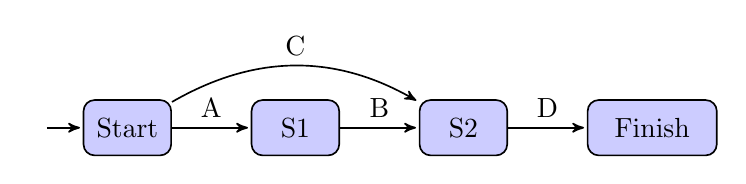
\begin{tikzpicture}[->,>=stealth',shorten >=1pt,auto,column sep=2.2cm,
                    semithick,initial text=]
  \node[initial,block] (s0) {Start};
  \node[block] (s1) [right=of s0] {S1};
  \node[block] (s2) [right=of s1] {S2};
  \node[bw] (s3) [right=of s2] {Finish};

  \path (s0) edge node {A} (s1)
        (s1) edge node {B} (s2)
        (s2) edge node {D} (s3)
        (s0) edge[bend left=30] node {C} (s2);
\end{tikzpicture}
\end{center}

\section*{Data and Task Parallelism}
There are two broad categories of paralellism: data parallelism and
task parallelism. An analogy to data parallelism is hiring a call
center to (incompetently) handle large volumes of support calls,
\emph{all in the same way}. Assembly lines are an analogy to task
parallelism: each worker does a \emph{different} thing.

More precisely, in data parallelism, multiple threads perform the
\emph{same} operation on separate data items. For instance, you have a
big array and want to double all of the elements. Assign part of the
array to each thread. Each thread does the same thing: double array
elements.

In task parallelism, multiple threads perform \emph{different}
operations on separate data items. So you might have a thread that
renders frames and a thread that compresses frames and combines them
into a single movie file.

We'll continue by looking at a number of parallelization patterns,
examples of how to apply them, and situations where they might apply.

\subsection*{Data Parallelism with SIMD}
The ``typical'' boring standard uniprocessor is Single Instruction Single Data (SISD) but since the mid-1980s we've had more options than that. We'll talk about single-instruction multiple-data (SIMD) later on in
this course, but here's a quick look. Each SIMD
instruction operates on an entire vector of data. These instructions
originated with supercomputers in the 70s. More recently, GPUs; the
x86 SSE instructions; the SPARC VIS instructions; and the
Power/PowerPC AltiVec instructions all implement SIMD.

\paragraph{Code.} Let's look at an application of SIMD instructions.

\begin{verbatim}
void vadd(double * restrict a, double * restrict b, int count) {
  for (int i = 0; i < count; i++)
    a[i] += b[i];
}
\end{verbatim}

Compiling this without SIMD on a 32-bit x86 ({\tt gcc -m32 -march=i386 -S}) might give this:
\begin{verbatim}
loop:
  fldl  (%edx)
  faddl (%ecx)
  fstpl (%edx)
  addl  8, %edx
  addl  8, %ecx
  addl  1, %esi
  cmp   %eax, %esi
  jle   loop
\end{verbatim}

We can instead compile to SIMD instructions ({\tt gcc -m32 -march=prescott -mfpmath=sse})
and get something like this:
\begin{verbatim}
loop:
  movupd (%edx),%xmm0
  movupd (%ecx),%xmm1
  addpd  %xmm1,%xmm0
  movpd  %xmm0,(%edx)
  addl   16,%edx
  addl   16,%ecx
  addl   2,%esi
  cmp    %eax,%esi
  jle    loop
\end{verbatim}
The \emph{packed} operations ({\tt p}) operate on multiple data
elements at a time (what kind of parallelism is this?)
The implication is that the loop only needs to loop half as many times.
Also, the instructions themselves are more efficient, because they're
not stack-based x87 instructions.

SIMD is different from the other types of parallelization we're
looking at, since there aren't multiple threads working at once.
It is complementary to using threads, and good for cases
where loops operate over vectors of data. These loops could also be
parallelized; multicore chips can do both, achieving high throughput.
SIMD instructions also work well on small data sets, where thread startup
cost is too high, while registers are just there to use.

We'll see a case study that uses SIMD (also known as vector
instructions) in Lecture 19. In~\cite{lemire18:_multic_simd}, Daniel Lemire argues that vector
instructions are, in general, a more efficient way to parallelize code
than threads. That is, when applicable, they use less overall CPU
resources (cores and power) and can even run faster.

\subsection*{Parallelization using Threads or Processes}
We'll be looking at thread-based or process-based parallelization for the
next bit. We don't care about the distinction between threads and processes
for the moment. In fact, we could even distribute work over multiple systems.

\paragraph{Pattern 1: Multiple Independent Tasks.} If you're just trying to maximize
system utilization, you can use one system to run a number of independent
tasks; for instance, you can put both a web server and database on
one machine. If the web server happens to be memory-bound while the
database is I/O-bound, then both can use system resources. If the web
server isn't talking to the database (rare these days!), then the tasks
would not get in each others' way.

Most services probably ought to be run under virtualization these
days, unless they're trivial or not mission-critical.

A more relevant example of multiple independent tasks occurs in
cluster/grid/cloud computing: the cloud might run a number of
independent tasks, and each node would run some of the tasks. The
cloud can retry a task (on a different node, perhaps) if it fails on
some node. Note that the performance ought to increase linearly with
the number of threads, since there shouldn't be communication between
the tasks.

\paragraph{Pattern 2: Multiple Loosely-Coupled Tasks.} Some applications contain
tasks which aren't quite independent (so there is some inter-task
communication), but not much.  In this case, the tasks may be
different from each other. The communication might be from the tasks
to a controller or status monitor; it would usually be asynchronous or
be limited to exceptional situations.

Refactoring an application this way can help with latency: if you 
split off the CPU-intensive computations into a sub-thread, then
the main thread can respond to user input more quickly.

Here's an example. Assume that an application needs to receive and
forward network packets, and also must log packet activity to disk.
Then the two tasks are clear: receive/forward, and log. Since logging
to disk is a high-latency event, a single-threaded application might
incur latency while writing to disk. Splitting into subtasks allows
the receive/forward to run without waiting for previous packets to be
logged, thus increasing the throughput of the system.

\paragraph{Pattern 3: Multiple Copies of the Same Task.} A common variant of
multiple independent tasks is multiple copies of the same task
(presumably on different data). In this case, we'd require there to be
no communication between the different copies, which would enable
linear speedup. An example is a rendering application running on
multiple distinct animations. We gain throughput, but need to wait
just as long for each task to complete.

\paragraph{Pattern 4: Single Task, Multiple Threads.} This is the classic
vision of ``parallelization'': for instance, distribute array
processing over multiple threads, and let each thread compute the
results for a subset of the array.

This pattern, unlike many of the others before it, can actually
decrease the time needed to complete a unit of work, since it gets
multiple threads involved in doing the single unit simultaneously.
The result is improved latency and therefore increased throughput.
Communication can be a problem, if the data is not nicely
array-structured, or has dependencies between different array parts.

Other names and variations for this pattern include ``fork-join'',
where the main process forks its execution and gives work to all of
the threads, with the join synchronizing threads and combining the
results; and ``divide-and-conquer'', where a thread spawns subthreads
to compute smaller and smaller parts of the solution.

\paragraph{Pattern 5: Pipeline of Tasks.} We've seen pipelining in the context of
computer architecture. It can also work for software. For instance,
you can use pipelining for packet-handling software, where multiple
threads, as above, might confound the order. If you use a three-stage
pipeline, then you can have three packets in-flight at the same time,
and you can improve throughput by a factor of 3 (given appropriate
hardware).  Latency would tend to remain the same or be worse (due to
communication overhead).

Some notes and variations on the pipeline: 1) if a stage is
particularly slow, then it can limit the performance of the entire
pipeline, if all of the work has to go through that stage; and 2) you
can duplicate pipeline stages, if you know that a particular stage is
going to be the bottleneck.

\paragraph{Pattern 6: Client-Server.} Botnets work this way (as does \verb+SETI@Home+,
etc). To execute some large computation, a server is ready to tell
clients what to do.  Clients ask the server for some work, and the
server gives work to the clients, who report back the results. Note
that the server doesn't need to know the identity of the clients for
this to work.

A single-machine example is a GUI application where the server part
does the backend, while the client part contains the user interface.
One could imagine symbolic algebra software being designed that way.
Window redraws are an obvious candidate for tasks to run on clients.

Note that the single server can arbitrate access to shared resources.
For instance, the clients might all need to perform network access.
The server can store all of the requests and send them out in an
orderly fashion.

The client-server pattern enables different threads to share work
which can somehow be parcelled up, potentially improving
throughput. Typically, the parallelism is somewhere between single
task, multiple threads and multiple loosely-coupled tasks. It's also a
design pattern that's easy to reason about.

\paragraph{Pattern 7: Producer-Consumer.} The producer-consumer is 
a variant on the pipeline and client-server models. In this case, the
producer generates work, and the consumer performs work. An example is
a producer which generates rendered frames, and a consumer which
orders these frames and writes them to disk. There can be any number
of producers and consumers. This approach can improve throughput
and also reduces design complexity.

\paragraph{Combining Strategies.} If one of the patterns suffices,
then you're done. Otherwise, you may need to combine strategies.
For instance, you might often start with a pipeline, and then 
use multiple threads in a particular pipeline stage to handle one
piece of data. Or, as I alluded to earlier, you can replicate
pipeline stages to handle different data items simultaneously.

Note also that you can get synergies between different patterns.
For instance, consider a task which takes 100 seconds. First, you
take 80 seconds and parallelize it 4 ways (so, 20 seconds). This
reduces the runtime to 40 seconds. Then, you can take the serial 
20 seconds and split it into two threads. This further reduces 
runtime to 30 seconds. You get a $2.5\times$ speedup from the
first transformation and $1.3\times$ from the second, if you do it
after the first. But, if you only did the second parallelization,
you'd only get a $1.1\times$ speedup.

\subsection*{How to Parallelize Code}
Here's a four-step outline of what you need to do.
\begin{enumerate}
\item Profile the code.
\item Find dependencies in hotspots. For each dependency chain in
a hotspot, figure out if you can execute the chain as
multiple parallel tasks or a loop over multiple parallel iterations.
Think about changing the algorithm, if that would help.
\item Estimate benefits. 
\item If they're not good enough (e.g. far from linear speedup),
step back and see if you can parallelize something else up the
call chain, or at a higher level of absraction.
(Think Mandelbrot sets and computing different points in parallel).
\end{enumerate}
Try to reduce the amount of synchronization that you have to do
(waiting for parallel tasks to finish), because that always slows
you down.

\section*{Thread Pools} We talked about ``single task, multiple threads''
above. The idea behind a \emph{thread pool} is that it's relatively
expensive to start a thread; it costs resources to keep the threads
running at the operating system level; and the threads won't run
optimally anyway, because they'll spend too much time swapping state
in and out of the cache.  Instead, you start an appropriate number of
threads, which each grab work from a work queue, do the work,
and report the results back. Web servers are a good application of
thread pools\footnote{Apache does this: \url{http://httpd.apache.org/docs/2.0/mod/worker.html}. Also see an assignment where the students write thread-pooled web servers: \url{http://www.cse.nd.edu/~dthain/courses/cse30341/spring2009/project4/project4.html}.}.

A key question is: how many threads should you create?  This depends
on which resources your threads use; if you are writing
computationally-intensive threads, then you probably want to have
fewer threads than the number of virtual CPUs. You can also use
Amdahl's Law to estimate the maximum useful number of threads, as
discussed previously.

Here's a longer discussion of thread pools:

\begin{center}
\url{http://www.ibm.com/developerworks/library/j-jtp0730.html}
\end{center}

Modern languages provide thread pools; Java's
\url{java.util.concurrent.ThreadPoolExecutor}~\cite{java:threadpoolexecutor}, C\#'s
\url{System.Threading.ThreadPool}~\cite{csharp:threadpool}, and GLib's {\tt GThreadPool}~\cite{gnome:threadpool} all implement thread pools. 

\paragraph{GLib.} 
GLib is a C library developed by the GTK team. It provides many useful
features that you might otherwise have to implement yourself in C.
%Consider using GLib's thread pool in your assignment 2, unless you
%want to implement the work queue yourself.  (I see no reason to do
%that!)









\chapter*{18 --- Reentrancy, Inlining, High-Level Languages}

\addcontentsline{toc}{chapter}{18 --- Reentrancy, Inlining, High-Level Languages}

\section*{Reentrancy}

Recall from a bit earlier the idea of a side effect of a function call. 

Code that allows multiple concurrent invocations without affecting the outcome is called reentrant or ``pure'' (and the use of the word pure shouldn't imply any sort of moral judgement on the code). It is a desirable property to have code that is reentrant if we want to parallelize things. If a function is not reentrant, it may not be possible to make it thread safe. And furthermore, a reentrant function cannot call a non-reentrant one (and maintain its status as reentrant).

Side effects are sort of undesirable, but not necessarily bad. Printing to console is unavoidably making use of a side effect, but it's what we want. Nevertheless, it should be obvious that when printing we can't have reentrant behaviour because two threads trying to write at the same time to the console would result in jumbled output. Or alternatively, restarting the print routine might result in some doubled characters on the screen.

The trivial example of a non-reentrant C function:
\begin{lstlisting}[language=C]
int tmp;

void swap( int x, int y ) {
    tmp = y;
    y = x;
    x = tmp;
}
\end{lstlisting}

Why is this non-reentrant? Because there is a global variable \texttt{tmp} and it is changed on every invocation of the function. We can make the code reentrant by moving the declaration of \texttt{tmp} inside the function, which would mean that every invocation is independent of every other. And thus it would be thread safe, too.

Remember that in things like interrupt subroutines (ISRs) having the code be reentrant is very important. Interrupts can get interrupted by higher priority interrupts and when that happens the ISR may simply be restarted (or we're going to break off handling what we're doing and call the same ISR in the middle of the current one). Either way, if the code is not reentrant we will run into problems.

Let us also draw a distinction between thread safe code and reentrant code. A thread safe operation is one that can be performed from more than one thread at the same time. On the other hand, a reentrant operation can be invoked while the operation is already in progress, possibly from within the same thread. Or it can be re-started without affecting the outcome. See this code example from~\cite{tont:threadsafe}:
\begin{lstlisting}[language=C]
int length = 0;
char *s = NULL;

// Note: Since strings end with a 0, if we want to
// add a 0, we encode it as "\0", and encode a
// backslash as "\\".


// WARNING! This code is buggy - do not use!


void AddToString(int ch)
{
  EnterCriticalSection(&someCriticalSection);
  // +1 for the character we're about to add
  // +1 for the null terminator
  char *newString = realloc(s, (length+1) * sizeof(char));
  if (newString) {
    if (ch == '\0' || ch == '\\') {
      AddToString('\\'); // escape prefix
    }
    newString[length++] = ch;
    newString[length] = '\0';
    s = newString;
  }
  LeaveCriticalSection(&someCriticalSection);
}
\end{lstlisting}

Is it thread safe? Sure - there is a critical section protected by the mutex \texttt{someCriticalSection}. But is is re-entrant? Nope. The internal call to \texttt{AddToString} causes a problem because the attempt to use \texttt{realloc} will use a pointer to \texttt{s} that is no longer valid (because it got stomped by the earlier call to \texttt{realloc}).

\subsection*{Functional Programming and Parallelization}
Interestingly, functional programming languages (by which I do NOT mean procedural programming languages like C) such as Haskell and Scala and so on, lend themselves very nicely to being parallelized. Why? Because a purely functional program has no side effects and they are very easy to parallelize. If a function is impure, its functions signature will indicate so. Thus spake Joel\footnote{``Thus Spake Zarathustra'' is a book by Nietzsche, and this was not a spelling error.}:

\begin{quote}
\textit{Without understanding functional programming, you can't invent MapReduce, the algorithm that makes Google so massively scalable. The terms Map and Reduce come from Lisp and functional programming. MapReduce is, in retrospect, obvious to anyone who remembers from their 6.001-equivalent programming class that purely functional programs have no side effects and are thus trivially parallelizable.}~\cite{joel:functional}
\end{quote}

This assumes of course that there is no data dependency between functions. Obviously, if we need a computation result, then we have to wait. 

Object oriented programming kind of gives us some bad habits in this regard: we tend to make a lot of \texttt{void} methods. In functional programming these don't really make sense, because if it's purely functional, then there are some inputs and some outputs. If a function returns nothing, what does it do? For the most part it can only have side effects which we would generally prefer to avoid if we can, if the goal is to parallelize things. 

\paragraph{C++: the functional version?} {\tt algorithms} has been part of C++ since C++11. It provides algorithm implementations as part of the standard library. Some of the algorithms are standard: {\tt sort}, {\tt reverse}, {\tt is\_heap}\ldots

What's new in C++17, though, is parallel and vectorized {\tt
algorithms}. You can specify an execution policy for these algorithms
({\tt sequenced\_policy}, {\tt parallel\_policy}, or {\tt
parallel\_unsequenced\_policy}). The compiler and runtime make it
so. (Or, they don't. As of this writing in 2018, mainstream C++
compilers don't support C++17 yet).

As part of this process, C++17 also introduced some new algorithms, such as
{\tt for\_each\_n}, {\tt exclusive\_scan}, and {\tt reduce}.
If you know functional programming (e.g. Haskell), these are also known as
{\tt map}, {\tt scanl}, and {\tt fold1/foldl1}.

Rainer Grimm writes more about these in blogposts from February and May of 2017:
\cite{grimm17:_paral_algor_stand_templ_librar} \cite{grimm17:_c}.


\section*{Good Programming Practices: Inlining}
We have seen the notion of inlining:
  \begin{itemize}
    \item Instructs the compiler to just insert the function code in-place,
      instead of calling the function.
    \item Hence, no function call overhead!
    \item Compilers can also do better---context-sensitive---operations they couldn't
      have done before.
  \end{itemize}

OK, so inlining removes overhead. Sounds like better performance! Let's inline everything!
There are two ways of inlining in C++.

\paragraph{Implicit inlining.} (defining a function inside a class definition):
  \begin{lstlisting}[language=C]
class P {
public:
    int get_x() const { return x; }
...
private:
    int x;
};
  \end{lstlisting}

\paragraph{Explicit inlining.} Or, we can be explicit:
  \begin{lstlisting}[language=C]
inline max(const int& x, const int& y) {
    return x < y ? y : x;
}
  \end{lstlisting}

\paragraph{The Other Side of Inlining.}
Inlining has one big downside:
  \begin{itemize}
    \item Your program size is going to increase.
  \end{itemize}
   This is worse than you think:
      \begin{itemize}
        \item Fewer cache hits.
        \item More trips to memory.
      \end{itemize}
   Some inlines can grow very rapidly (C++ extended constructors).
  Just from this your performance may go down easily.

  Note also that inlining is merely a suggestion to compilers~\cite{gcc:inlining}.
  They may ignore you.
  For example:
  \begin{itemize}
    \item taking the address of an ``inline'' function and using it; or
    \item virtual functions (in C++),
  \end{itemize}
  will get you ignored quite fast.

\paragraph{Implications of inlining.} Inlining can make your life worse in two ways.
First, debugging is more difficult (e.g. you can't set a breakpoint in a function that
  doesn't actually exist).
 Most compilers simply won't inline code with debugging symbols on.
 Some do, but typically it's more of a pain.

Second, it can be a problem for library design:
  \begin{itemize}
    \item If you change any inline function in your library, any users
      of that library have to {\bf recompile} their program if the
      library updates. (Congratulations, you made a non-binary-compatible change!)
  \end{itemize}
This would not be a problem for non-inlined functions---programs execute the new function
dynamically at runtime.

\section*{High-Level Language Performance Tweaks}
So far, we've only seen C---we haven't seen anything complex, and C is
low level, which is good for learning what's really going on.

 Writing compact, readable code in C is hard, especially when \#define
macros and {\tt void *} beckon.

    C++11 has made major strides towards readability and
    efficiency---it provides light-weight abstractions. We'll look at
    a couple of examples.

\paragraph{Sorting.} Our goal is simple: we'd like to sort a bunch of integers.
In C, you would usually just use qsort from {\tt stdlib.h}.

  \begin{lstlisting}
void qsort (void* base, size_t num, size_t size,
            int (*comparator) (const void*, const void*));
  \end{lstlisting}

This is a fairly ugly definition (as usual, for generic C functions). How ugly is it?
Let's look at a usage example.
  \begin{lstlisting}[language=C]
#include <stdlib.h>

int compare(const void* a, const void* b)
{
    return (*((int*)a) - *((int*)b));
}

int main(int argc, char* argv[])
{
    int array[] = {4, 3, 5, 2, 1};
    qsort(array, 5, sizeof(int), compare);
}
  \end{lstlisting}
This looks like a nightmare, and is more likely to have bugs than what we'll see next.


C++ has a sort with a much nicer interface\footnote{\ldots well, nicer to use, after you get over templates.}:

  \begin{lstlisting}[language=C++]
template <class RandomAccessIterator>
void sort (
    RandomAccessIterator first,
    RandomAccessIterator last
);

template <class RandomAccessIterator, class Compare>
void sort (
    RandomAccessIterator first,
    RandomAccessIterator last,
    Compare comp
);
  \end{lstlisting}
It is, in fact, easier to use:
  \begin{lstlisting}[language=C++]
#include <vector>
#include <algorithm>

int main(int argc, char* argv[])
{
    std::vector<int> v = {4, 3, 5, 2, 1};
    std::sort(v.begin(), v.end());
}
  \end{lstlisting}

{\bf Note:} Your compare function can be a function or a functor. (Don't know what functors
are? In C++, they're functions with state.) By default,
  {\tt sort} uses {\tt operator$<$} on the objects being sorted.

  \begin{itemize}
    \item Which is less error prone?
    \item Which is {\bf faster}?
  \end{itemize}

The second question is empirical. Let's see. We generate an array of 2 million ints
and sort it (10 times, taking the average).

\begin{itemize}
\item qsort: 0.49 seconds
\item C++ sort: 0.21 seconds
\end{itemize}

The C++ version is {\bf twice} as fast. Why?
      \begin{itemize}
        \item The C version just operates on memory---it has no clue about the
          data.
        \item We're throwing away useful information about what's being sorted.
        \item A C function-pointer call prevents inlining of the compare function.
      \end{itemize}
OK. What if we write our own sort in C, specialized for the data?

\begin{itemize}
\item Custom C sort: 0.29 seconds
\end{itemize}

Now the C++ version is still faster (but it's close). But, this is
quickly going to become a maintainability nightmare.
      \begin{itemize}
        \item Would you rather read a custom sort or 1 line?
        \item What (who) do you trust more?
      \end{itemize}

\subsection*{Lesson}
Abstractions will not make your program slower. 

\noindent
They allow speedups and are much easier to maintain and read.

\subsection*{Vectors vs Lists}
Consider two
problems.

\begin{enumerate}
\item Generate {\bf N} random integers and insert them into (sorted)
      sequence.
      
      {\bf Example:} 3 4 2 1
      
      \begin{itemize}
        \item 3
        \item 3 4
        \item 2 3 4
        \item 1 2 3 4
      \end{itemize}

\item Remove {\bf N} elements one-at-a-time by going to a random position
      and removing the element.

      {\bf Example:} 2 0 1 0
      
      \begin{itemize}
        \item 1 2 4
        \item 2 4
        \item 2
        \item 
      \end{itemize}
\end{enumerate}

For which {\bf N} is it better to use a list than a vector (or array)?

 
\paragraph{Complexity analysis.} As good computer scientists, let's analyze
the complexity.  

{\bf Vector}:\\[-2em]
      \begin{itemize}
        \item Inserting\\[-2em]
          \begin{itemize}
            \item $O(\log n)$ for binary search
            \item $O(n)$ for insertion (on average, move half the elements)
          \end{itemize}
        \item Removing\\[-2em]
          \begin{itemize}
            \item $O(1)$ for accessing
            \item $O(n)$ for deletion (on average, move half the elements)
          \end{itemize}
      \end{itemize}

{\bf List}:\\[-2em]
      \begin{itemize}
        \item Inserting\\[-2em]
          \begin{itemize}
            \item $O(n)$ for linear search
            \item $O(1)$ for insertion
          \end{itemize}
        \item Removing\\[-2em]
          \begin{itemize}
            \item $O(n)$ for accessing
            \item $O(1)$ for deletion
          \end{itemize}
      \end{itemize}

Therefore, based on their complexity, lists should be better.

\paragraph{Reality.} OK, here's what happens. 
\begin{verbatim}
$ ./vector_vs_list 50000
Test 1
======
vector: insert 0.1s   remove 0.1s   total 0.2s
list:   insert 19.44s   remove 5.93s   total 25.37s
Test 2
======
vector: insert 0.11s   remove 0.11s   total 0.22s
list:   insert 19.7s   remove 5.93s   total 25.63s
Test 3
======
vector: insert 0.11s   remove 0.1s   total 0.21s
list:   insert 19.59s   remove 5.9s   total 25.49s
\end{verbatim}

{\bf Vectors} dominate lists, performance wise. Why?
  \begin{itemize}
    \item Binary search vs. linear search complexity dominates.
    \item Lists use far more memory.
      {\bf On 64 bit machines:}
      \begin{itemize}
        \item Vector: 4 bytes per element.
        \item List: At least 20 bytes per element.
      \end{itemize}
    \item Memory access is slow, and results arrive in blocks:
      \begin{itemize}
        \item Lists' elements are all over memory, hence many
          cache misses.
        \item A cache miss for a vector will bring a lot more usable data.
      \end{itemize}
  \end{itemize}

So, here are some tips for getting better performance.
  \begin{itemize}
    \item Don't store unnecessary data in your program.
    \item Keep your data as compact as possible.
    \item Access memory in a predictable manner.
    \item Use vectors instead of lists by default.
    \item Programming abstractly can save a lot of time.
    \item Often, telling the compiler more gives you better code.
    \item Data structures can be critical, sometimes more than complexity.
    \item {\bf Low-level code != Efficient}.
    \item Think at a low level if you need to optimize anything.
    \item Readable code is good code---different hardware needs different
      optimizations.
  \end{itemize}










\chapter*{19 --- Performance Case Studies}

\addcontentsline{toc}{chapter}{19 --- Performance Case Studies}

\section*{Making Firefox Fast}

Let's look at Mike Conley's Firefox Performance Updates,
\begin{center}
{\scriptsize
\vspace*{-1em}
\url{https://mikeconley.ca/blog/2018/02/14/firefox-performance-update-1/}
}
\end{center}
\vspace*{-1em}

\begin{itemize}[noitemsep]
\item don't use CPU animating out-of-view elements
\item move db init off main thread
\item keep better profiling data
\item parallel painting for macOS
\item lazily instantiate Search Service only when first search starts
\item halve size of the blocklist
\item refactor to reduce main-thread IO
\item don't hold all frames of animated GIFs/APNGs in memory
\item eliminate an unnecessary hash table
\item use more modern compiler
\end{itemize}

We can categorize most of these updates into the categories we've seen before:
\begin{itemize}[noitemsep]
\item do less work\\
 (or do it sooner/later);
\item use threads (move work off main thread);
\item track performance;
\end{itemize}
Which of the updates fall into which categories?

\subsection*{Tab warming} We continue by examining one particular update, \emph{tab warming}, in detail:
\begin{center}
\scriptsize
\vspace*{-1em}
\url{https://mikeconley.ca/blog/2018/01/11/making-tab-switching-faster-in-firefox-with-tab-warming/}.
\end{center}
\vspace*{-1em}

\hfill ``Maybe this is my Canadian-ness showing, but I like to think of it almost like coming in from shoveling snow off of the driveway, and somebody inside has \emph{already made hot chocolate for you}, because they knew you’d probably be cold.'' --- Mike Conley

Consider switching tabs. Previously, Firefox would request a paint of the newly-selected tab and wait for the rendering to be available before switching the tab.

The idea is to reduce user-visible latency by predicting an imminent tab switch. How do you know that the user is about to switch tabs? When the user has a mouse, then the mouse cursor will hover over the next tab.

\begin{quote}
Assuming a sufficiently long delay between hover and click, the tab switch should be perceived as instantaneous. If the delay was non-zero but still not long enough, we will have nonetheless shaved that time off in eventually presenting the tab to you.

And in the event that we were wrong, and you weren’t interested in seeing the tab, we eventually throw the uploaded layers away.
\end{quote}

The blog post does not report performance numbers (but bug 1430160 discusses how to collect them).

\subsection*{Firefox in general}

Try: ``about:mozilla'' in Firefox. On a Quantum Flow-enabled version, you'll see

\begin{center}
\emph{The Beast adopted new raiment and studied the ways of Time and Space and Light and the Flow of energy through the Universe. From its studies, the Beast fashioned new structures from oxidised metal and proclaimed their glories. And the Beast’s followers rejoiced, finding renewed purpose in these teachings.}

\hfill \emph{from The Book of Mozilla, 11:14}
\end{center}

In 2017, Mozilla released Electrolysis
(E10s\footnote{\url{https://blog.mozilla.org/blog/2017/06/13/faster-better-firefox/}}),
which leverages multicore processors by using multiple OS-level
processes. (Chrome has always done this, but Firefox attempts to also
keep memory usage
down\footnote{\url{https://medium.com/mozilla-tech/the-search-for-the-goldilocks-browser-and-why-firefox-may-be-just-right-for-you-1f520506aa35}}.)
Beyond internal architecture issues, handling Add-Ons (now
WebExtensions) was perhaps the most challenging part of going
multi-process.

Note the connection to different thread/process models.
Chrome is one-process-per-tab, while Firefox multiplexes tabs across
the 4 content processes (``hardware threads'', by analogy). Limiting
the number of tabs also limits the memory consumption of the browser:
we don't have arbitrary numbers of renderer state.

\begin{center}
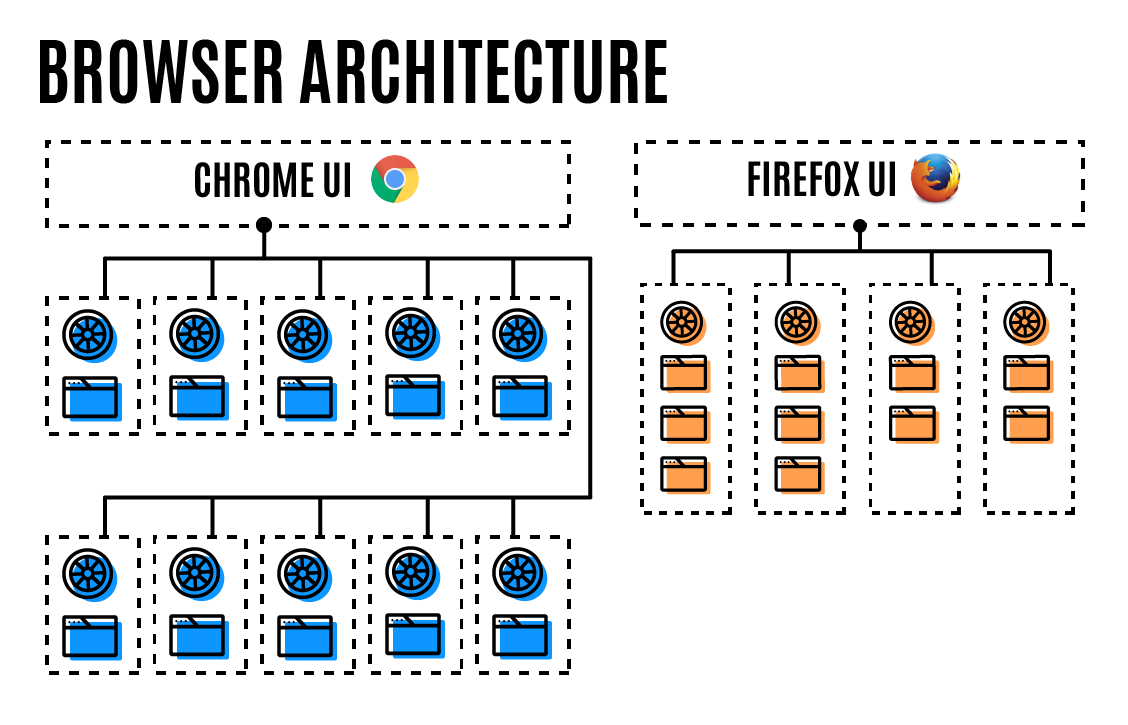
\includegraphics[width=.9\textwidth]{images/L19-chrome-vs-firefox.png}
\end{center}
Source: Ryan Pollock, ``The search for the Goldilocks browser and why Firefox might be `just right' for you'', \\
{\scriptsize \url{https://medium.com/mozilla-tech/the-search-for-the-goldilocks-browser-and-why-firefox-may-be-just-right-for-you-1f520506aa35}}

As a crude summary, Electrolysis works on splitting across processes
while the newer Quantum Flow leverages multithreading and other
improvements.  Quantum Flow uses the Rust programming language and its
``fearless concurrency'' (in Rust-speak). Rust should probably be part
of a future revision of the ECE 459 curriculum. But we'll focus on
Firefox here.

\subsection*{Quantum Flow}
Here's a retrospective of the Quantum Flow project:
\begin{center}
\url{https://ehsanakhgari.org/blog/2017-09-21/quantum-flow-engineering-newsletter-25}
\end{center}

To sum up, they formed a small term and did the following.
\begin{enumerate}[noitemsep]
\item Measure slowness: gather information, instrument Firefox, collect profiling data and measurements. Prioritize issues.
\item Gather help: convince other teams to pitch in with perf improvements. Examples: front-end team (reduce flushes, timers); layout team (reflow performance).
\item Fix all the things! (Or at least the most important ones).
\end{enumerate}
Given the short timeline they gave themselves (6 months) and the limited resources, an important part of their work was convincing others to help.
They triaged 895 bugs and fixed 369 of them. The weekly Quantum Flow Engineering Newsletter was a key motivational tool.

After the project wound down, they aimed to distribute responsibility for perf improvements across the entire project.

\section*{Firefox Telemetry}
Firefox's Telemetry feature collects lots of information from Firefox
users.  Idea: collect data before hacking away at things.  Firefox collects hundreds of
gigabytes of anonymous metrics per day while browsing and makes it all available to
the public.  One can view this as an analogy of CPU profiling on a
massively distributed context. This data is collected much less often than
CPU profiling data but at a much broader scope.
\begin{center}
\url{https://telemetry.mozilla.org/}
\end{center}
If you are running Firefox and want to see what it is collecting:
\begin{center}
\url{about:telemetry}
\end{center}

You can view distributions of telemetry probes (in the form of
histograms). You can also make your own dashboard based on Firefox
Telemetry data and Mozilla has infrastructure for their developres to
formulate and evaluate their own queries.

Example questions:
\begin{itemize}[noitemsep]
\item Is Firefox the user's default browser? (69\% yes)
\item Does e10s make startup faster? (no, slower)
\item Which plugins tend to freeze the browser on load? (Silverlight and Flash)
\end{itemize}
Can see evolution of data over time.

Firefox developers can propose new telemetry probes which are reviewed
for data privacy\footnote{Mozilla Data Collection Practices: \url{https://wiki.mozilla.org/Firefox/Data_Collection}} as well as through normal code review channels.

\paragraph{Pings.} Firefox phones the data home using so-called ``pings''.
Firefox sends a ``main ping'' every 24 hours, upon shutdown, environment change,
and crash. There are other types of pings as well. Pings get sent either by Firefox
or by a helper program, Pingsender, when Firefox isn't running. Presumably they
are sent over the network as compressed JSON to a central server.

Here's the common ping structure:

\begin{verbatim}
{
  type: <string>, // "main", "activation", "optout", "saved-session", ...
  id: <UUID>, // a UUID that identifies this ping
  creationDate: <ISO date>, // the date the ping was generated
  version: <number>, // the version of the ping format, currently 4

  application: {
    architecture: <string>, // build architecture, e.g. x86
    buildId: <string>, // "20141126041045"
    name: <string>, // "Firefox"
    version: <string>, // "35.0"
    displayVersion: <string>, // "35.0b3"
    vendor: <string>, // "Mozilla"
    platformVersion: <string>, // "35.0"
    xpcomAbi: <string>, // e.g. "x86-msvc"
    channel: <string>, // "beta"
  },

  clientId: <UUID>, // optional
  environment: { ... }, // optional, not all pings contain the environment
  payload: { ... }, // the actual payload data for this ping type
}
\end{verbatim}

Pings contain scalars (counts, booleans, strings) and histograms. A histogram collects
bucketed data (think grade distributions). Both scalars and histograms can be keyed, e.g.
how often searches happen for which search engines.



\section*{Single-Thread Performance}

\hfill ``Can you run faster just by trying harder?''

The performance improvements we've seen to date have been leveraging parallelism
to improve throughput. Decreasing latency is trickier---it often requires domain-specific
tweaks. Tab warming decreses latency but doesn't increase overall throughput.

Sometimes it's classic computer science: Quantum Flow found a place
where they could cache the last element of a list to reduce time
complexity for insertion from $O(n^2)$ to $O(n \log n)$.

\begin{center}
\url{https://bugzilla.mozilla.org/show_bug.cgi?id=1350770}
\end{center}

We'll also look at a more involved example of decreasing latency today, Stream VByte~\cite{LEMIRE20181}.
Even this example leverages parallelism---it uses vector instructions. But there
are some sequential improvements, e.g. Stream VByte takes care to be predictable
for the branch predictor.

\paragraph{Context.} We can abstract the problem to that of storing a sequence of small integers.
Such sequences are important, for instance, in the context of inverted indexes, which allow
fast lookups by term, and support boolean queries which combine terms.

Here is a list of documents and some terms that they contain:
\begin{center}
\begin{tabular}{r|l}
docid & terms \\ \hline
1 & dog, cat, cow\\
2 & cat\\
3 & dog, goat\\
4 & cow, cat, goat\\
\end{tabular}
\end{center}

The inverted index looks like this:
\begin{center}
\begin{tabular}{r|l}
term & docs \\ \hline
dog & 1, 3 \\
cat & 1, 2, 4 \\
cow & 1, 4 \\
goat & 3, 4
\end{tabular}
\end{center}

Inverted indexes contain many small integers in their lists: it is
sufficient to store the delta between a doc id and its successor, and
the deltas are typically small if the list of doc ids is sorted.
(Going from deltas to original integers takes time logarithmic
in the number of integers).

VByte is one of a number of schemes that use a variable number of
bytes to store integers.  This makes sense when most integers are
small, and especially on today's 64-bit processors.

VByte works like this:
\vspace*{-1em}
\begin{itemize}[noitemsep]
\item $x$ between 0 and $2^7-1$, e.g. $17 = 0b10001$: $0xxx xxxx$, e.g. $0001 0001$;
\item $x$ between $2^7$ and $2^{14}-1$, e.g. $1729 = 0b110 11000001$:
                   $1xxx xxxx/0xxx xxxx$, e.g. $1100 0001/0000 1101$;
\item $x$ between $2^{14}$ and $2^{21}-1$: $0xxx xxxx/1xxx xxxx/1xxx xxxx$;
\item etc.
\end{itemize}
That is, the control bit, or high-order bit, is 0 if you have finished representing the integer,
and 1 if more bits remain. (UTF-8 encodes the length, from 1 to 4, in high-order bits of the first byte.)

It might seem that dealing with variable-byte integers might be
harder than dealing fixed-byte integers, and it is. But there are performance benefits: because we are
using fewer bits, we can fit more information into our limited RAM and
cache, and even get higher throughput. Storing and reading 0s isn't an effective
use of resources. However, a naive algorithm to decode VByte also gives
lots of branch mispredictions.

Stream VByte is a variant of VByte which works using SIMD instructions.
Science is incremental, and Stream VByte builds on earlier work---masked VByte
as well as {\sc varint}-GB and {\sc varint}-G8IU. The innovation in
Stream VByte is to store the control and data streams separately.

Stream VByte's control stream uses two bits per integer to represent the size of the integer:
\begin{center}
\vspace*{-1em}
\begin{tabular}{ll@{~~~~~~~~}ll}
00 & 1 byte & 10 & 3 bytes\\
01 & 2 bytes & 11 & 4 bytes
\end{tabular}
\end{center}

Each decode iteration reads a byte from the control stream and 16 bytes of data from memory.
It uses a lookup table over the possible values of the control stream to decide how many
bytes it needs out of the 16 bytes it has read, and then uses SIMD instructions to shuffle
the bits each into their own integers. Note that, unlike VByte, Stream VByte uses all 8 bits
of each data byte as data.

For instance, if the control stream contains $0b1000~1100$, then the data stream
contains the following sequence of integer sizes: $3, 1, 4, 1$. Out of the 16 bytes read,
this iteration will use 9 bytes; it advances the data pointer by 9. It then uses the SIMD
``shuffle'' instruction to put the decoded integers from the data stream at known positions in the
128-bit SIMD register; in this case, it pads the first 3-byte integer with 1 byte, then
the next 1-byte integer with 3 bytes, etc. Let's say that the input is
{\tt 0xf823~e127~2524~9748~1b..~....~....~....}. The 128-bit output is
{\tt 0x00f8~23e1/0000~0027/2524 9748/0000/001b}, with the /s denoting separation
between outputs. The shuffle mask is precomputed and, at
execution time, read from an array.

The core of the implementation uses three SIMD instructions:
\begin{lstlisting}[language=C]
  uint8_t C = lengthTable[control];
  __m128i Data = _mm_loadu_si128 ((__m128i *) databytes);
  __m128i Shuf = _mm_loadu_si128(shuffleTable[control]);
  Data = _mm_shuffle_epi8(Data, Shuf);
  databytes += C; control++;
\end{lstlisting}

\paragraph{Discussion.} The paper~\cite{LEMIRE20181} includes a number of benchmark results
showing how Stream VByte performs better than previous techniques on a realistic input.
Let's discuss how it achieves this performance.

\begin{itemize}[noitemsep]
\item control bytes are sequential: the processor can always prefetch the next control byte, because
its location is predictable;
\item data bytes are sequential and loaded at high throughput;
\item shuffling exploits the instruction set so that it takes 1 cycle;
\item control-flow is regular (executing only the tight loop which retrieves/decodes control
and data; there are no conditional jumps).
\end{itemize}
We're exploiting SIMD, so this isn't quite strictly single-threaded performance.
Considering branch prediction and caching issues, though,
certainly improves single-threaded performance.










\chapter*{20 --- Compiler Optimizations}

\addcontentsline{toc}{chapter}{20 --- Compiler Optimizations}

\section*{Compiler Optimizations}

\hfill ``Is there any such thing as a free lunch?''

Compiler optimizations really do feel like a free lunch.
But what does it really mean when you say {\tt -O2}?
We'll see some representative compiler optimizations and discuss how
they can improve program performance. Because we're talking about
Programming for Performance, I'll point out cases that stop compilers
from being able to optimize your code. In general, it's better if the
compiler automatically does a performance-improving transformation
rather than you doing it manually; it's probably a waste of time for
you and it also makes your code less readable.

Many pages on the Internet describe
optimizations. Here's one that contains good examples:

$\qquad \qquad$ \url{http://www.digitalmars.com/ctg/ctgOptimizer.html}

You can find a full list of {\tt gcc} options here:

$\qquad \qquad$ \url{http://gcc.gnu.org/onlinedocs/gcc/Optimize-Options.html}

\paragraph{About Compiler Optimizations.} First of all, ``optimization'' is
a bit of a misnomer, since compilers generally do not generate ``optimal'' code.
They just generate \emph{better} code.

Often, what happens is that the program you literally wrote is too slow. The
contract of the compiler (working with the architecture) is to actually execute
a program with the same behaviour as yours, but which runs faster.

\paragraph{{\tt gcc} optimization levels.} Here's what {\tt -On} means for
{\tt gcc}. Other compilers have similar (but not identical) optimization flags.

\begin{itemize}[noitemsep]
\item {\tt -O0} (default): Fastest compilation time. Debugging works as expected.
\item {\tt -O1} ({\tt -O}): Reduce code size and execution time.
 No optimizations that increase compiliation time.
\item {\tt -O2}: All optimizations except space vs. speed tradeoffs.
\item {\tt -O3}: All optimizations.
\item {\tt -Ofast}: All {\tt -O3} optimizations, plus non-standards compliant optimizations,
      particularly {\tt -ffast-math}. (Like {\tt -fast} on the Solaris compiler.)\\[1em]
  This flag turns off exact implementations of IEEE or ISO rules/specifications for math
  functions. Generally, if you don't care about the exact result, you can use this for
  a speedup.
\end{itemize}

\subsection*{Scalar Optimizations}
By scalar optimizations, I mean optimizations
which affect scalar (non-array) operations. Here are some examples of scalar
optimizations.

\paragraph{Constant folding.} Probably the simplest optimization one can think of.
Tag line: ``Why do later something you can do now?'' We simply translate:

\begin{center}
\vspace*{-1em}
\begin{tabular}{lll}
i = 1024 * 1024 &
$\Longrightarrow$ &
i = 1048576
\end{tabular}
\end{center}

\noindent \emph{Enabled at all optimization levels.} The compiler will not emit
code that does the multiplication at runtime. It will simply use the
computed value.

\paragraph{Common subexpression elimination.} We can do common subexpression elimination
when the same expression {\tt x op y} is computed more than once, and
neither {\tt x} nor {\tt y} change between the two computations. In the
below example, we need to compute {\tt c + d} only once.


\begin{lstlisting}[language=C]
   a = (c + d) * y;
   b = (c + d) * z;

   w = 3;
   x = f(); y = x;
   z = w + y;

\end{lstlisting}


\noindent \emph{Enabled at {\tt -O2}, {\tt -O3} or with {\tt -fgcse}.} 
These flags actually enable a global (i.e. across-basic-blocks) CSE pass.
This also enables global constant and copy propagation.

\paragraph{Constant propagation.} Moves constant values from definition to
use. The transformation is valid if there are no redefinitions of the
variable between the definition and its use. In the above example,
we can propagate the constant value 3 to its use in {\tt z = w + y},
yielding {\tt z = 3 + y}.

\paragraph{Copy propagation.} A bit more sophisticated than constant
propagation---telescopes copies of variables from their definition to
their use. This usually runs after CSE. Using it, we can replace the
last statement with {\tt z = w + x}. If we run both constant and copy
propagation together, we get {\tt z = 3 + x}.

These scalar optimizations are more complicated in the presence
of pointers, e.g. {\tt z = *w + y}. More next time.

%\paragraph{Scalar Replacement of Aggregates.} Censored. Too many people misunderstood it last year.

\paragraph{Redundant Code Optimizations.} In some sense, most optimizations
remove redundant code, but one particular optimization is \emph{dead code
elimination}, which removes code that is guaranteed to not execute.
For instance:

{\scriptsize
\begin{center}
\vspace*{-2em}
\begin{minipage}{.3\textwidth}
\begin{lstlisting}[language=C]
  int f(int x) {
    return x * 2;
  }
  \end{lstlisting}
  \end{minipage} \begin{minipage}{.3\textwidth}
\begin{lstlisting}[language=C]
  int g() {
    if (f(5) % 2 == 0) {
      // do stuff...
    } else {
      // do other stuff
    }
  }
\end{lstlisting}
\end{minipage}
\end{center}
}
We see that the then-branch in {\tt g()} is always going to execute, and the
else-branch is never going to execute.

The general problem, as with many other compiler problems, is undecidable. Let's not get too caught up in the semantics of the \textit{Entscheidungsproblem}, even if you do speak German and like to show it off by pronouncing that word correctly.

\subsection*{Loop Optimizations}
Loop optimizations are particularly profitable when loops execute
often. This is often a win, because programs spend a lot of time looping.
The trick is to find which loops are going to be the important ones.
Profiling is helpful.

A loop induction variable is a variable that varies on each iteration
of the loop; the loop variable is definitely a loop induction variable,
but there may be others. \emph{Induction variable elimination} gets
rid of extra induction variables.

\emph{Scalar replacement} replaces an array read {\tt a[i]}
occuring multiple times with a single read {\tt temp = a[i]} and references
to {\tt temp} otherwise. It needs to know that {\tt a[i]} won't change
between reads.

Sane languages include array bounds checks, and loop optimizations
can eliminate array bounds checks if they can prove that the loop
never iterates past the array bounds.

\paragraph{Loop unrolling.} This optimization
lets the processor run more code without having to branch
as often. \emph{Software pipelining} is a synergistic optimization,
which allows multiple iterations of a loop to proceed in parallel.
This optimization is also useful for SIMD. Here's an example.
\begin{center}
\vspace*{-1em}
\begin{minipage}{.3\textwidth}
  \begin{lstlisting}[language=C]
for (int i = 0; i < 4; ++i)
    f(i)
  \end{lstlisting}
  \end{minipage} $\Longrightarrow \hspace*{2em}$ \begin{minipage}{.4\textwidth}
  \begin{lstlisting}[language=C]
f(0); f(1); f(2); f(3);
  \end{lstlisting}
  \end{minipage}
  \end{center}
\noindent \emph{Enabled with {\tt -funroll-loops}.}

\paragraph{Loop interchange.} This optimization can give big wins
for caches (which are key); it changes the nesting of loops to
coincide with the ordering of array elements in memory. For instance,
in C:
\begin{center}
\vspace*{-1em}
\begin{minipage}{.3\textwidth}
  \begin{lstlisting}[language=C]
for (int i = 0; i < N; ++i)
    for (int j = 0; j < M; ++j)
        a[j][i] = a[j][i] * c
  \end{lstlisting}
  \end{minipage} $\Longrightarrow \hspace*{2em}$ \begin{minipage}{.4\textwidth}
  \begin{lstlisting}[language=C]
for (int j = 0; j < M; ++j)
    for (int i = 0; i < N; ++i)
        a[j][i] = a[j][i] * c
  \end{lstlisting}
  \end{minipage}
  \end{center}
  since C is \emph{row-major} (meaning a[1][1] is beside a[1][2]),
rather than \emph{column-major}.

\noindent
\emph{Enabled with {\tt -floop-interchange}.}

Strangely enough, sometimes you want to do things the column-major way even though it's ``wrong''. If your two dimensional array is of an appropriate size then by intentionally hitting things in the ``wrong'' order, you'll trigger all your page faults up front and load all your pages into cache and then you can go wild. This was suggested as a way to make matrix multiplication faster for a sufficiently large matrix...

\paragraph{Loop fusion.} This optimization is like the OpenMP collapse
construct; we transform
\begin{center}
\vspace*{-1em}
\begin{minipage}{.3\textwidth}
  \begin{lstlisting}[language=C]
for (int i = 0; i < 100; ++i)
    a[i] = 4

for (int i = 0; i < 100; ++i)
    b[i] = 7
  \end{lstlisting}
  \end{minipage} $\Longrightarrow \hspace*{2em}$ \begin{minipage}{.4\textwidth}
  \begin{lstlisting}[language=C]
for (int i = 0; i < 100; ++i) {
    a[i] = 4
    b[i] = 7
}
  \end{lstlisting}
  \end{minipage}
  \end{center}
There's a trade-off between data locality and loop overhead; hence,
sometimes the inverse transformation, \emph{loop fission}, will
improve performance.

\paragraph{Loop-invariant code motion.} Also known as \emph{Loop hoisting},
this optimization moves calculations out of a loop. 
\begin{center}
\vspace*{-1em}
\begin{minipage}{.3\textwidth}
  \begin{lstlisting}[language=C]
for (int i = 0; i < 100; ++i) {
    s = x * y;
    a[i] = s * i;
}
  \end{lstlisting}
  \end{minipage} $\Longrightarrow \hspace*{2em}$ \begin{minipage}{.4\textwidth}
  \begin{lstlisting}[language=C]
s = x * y;
for (int i = 0; i < 100; ++i) {
    a[i] = s * i;
}
  \end{lstlisting}
  \end{minipage}
  \end{center}

This reduces the amount of work we have to do for each iteration of the loop.


\subsection*{Miscellaneous Low-Level Optimizations}
Some optimizations affect low level code generation; here are two examples.

\paragraph{Branch Prediction.} {\tt gcc} attempts to guess the probability of each branch to
best order the code. (For an {\tt if}, fall-through is most efficient. Why?)

This isn't quite an optimization, but you can use {\tt
  \_\_builtin\_expect(expr, value)} to help GCC, if you know the
run-time characteristics of your program. An example, from the
  Linux kernel:

  \begin{lstlisting}[language=C]
#define likely(x)       __builtin_expect((x),1)
#define unlikely(x)     __builtin_expect((x),0)
  \end{lstlisting}

\paragraph{Architecture-Specific.} {\tt gcc} can also generate code tuned to particular
processors and processor variants. You can specify this using {\tt
  -march} and {\tt -mtune}. ({\tt -march} implies {\tt -mtune}).
This will enable specific instructions that not all CPUs support (e.g. SSE4.2).
For example, {\tt -march=corei7}.

\noindent
Good to use on your local machine or your cloud servers, not ideal for code you ship to others.


\section*{Interprocedural Analysis and Link-Time Optimizations}
\hfill ``Are economies of scale real?''

In this context, does a
whole-program optimization really improve your program?
We'll start by first talking about some information that is critical for
whole-program optimizations.

\subsection*{Alias and Pointer Analysis}
As we've seen in the above analyses, compiler optimizations often need
to know about what parts of memory each statement reads to.  This is
easy when talking about scalar variables which are stored on the
stack. This is much harder when talking about pointers or arrays
(which can alias). \emph{Alias analysis} helps by declaring that a
given variable {\tt p} does not alias another variable {\tt q}; that
is, they point to different heap locations. \emph{Pointer analysis}
abstractly tracks what regions of the heap each variable points to.
A region of the heap may be the memory allocated at a particular
program point.

When we know that two pointers don't alias, then we know that their
effects are independent, so it's correct to move things around.
This also helps in reasoning about side effects and enabling reordering.

We've talked about automatic parallelization previously in this course.
At this point, I'll remind you that we used {\tt restrict} so that the
compiler wouldn't have to do as much pointer analysis. Shape analysis
builds on pointer analysis to determine that data structures are indeed
trees rather than lists.

\paragraph{Call Graphs.} Many interprocedural analyses require accurate
call graphs. A call graph is a directed graph showing relationships between
functions. It's easy to compute a call graph when you have C-style
function calls. It's much harder when you have virtual methods, as in
C++ or Java, or even C function pointers. In particular, you need pointer
analysis information to construct the call graph.

\paragraph{Devirtualization.} This optimization attempts to convert
virtual function calls to direct calls.  Virtual method calls have the
potential to be slow, because there is effectively a branch to
predict. If the branch prediction goes well, then it doesn't impose
more runtime cost. However, the branch prediction might go poorly.  (In
general for C++, the program must read the object's vtable.) Plus, virtual
calls impede other optimizations. Compilers can help by doing
sophisticated analyses to compute the call graph and by replacing
virtual method calls with nonvirtual method calls.  Consider the
following code:
  \begin{lstlisting}[language=C]
class A {
    virtual void m();
};

class B : public A {
    virtual void m();
}

int main(int argc, char *argv[]) {

    std::unique_ptr<A> t(new B);
    t.m();
}
  \end{lstlisting}
Devirtualization could eliminate vtable access; instead, we could just call B's {\tt m} method
directly. By the way, ``Rapid Type Analysis'' analyzes the entire program, observes that
only {\tt B} objects are ever instantiated, and enables devirtualization
of the {\tt b.m()} call.

\noindent \emph{Enabled with {\tt -O2}, {\tt -O3}, or with {\tt -fdevirtualize}.}

\paragraph{Inlining.} We talked about inlining in Lecture 18. Compilers can inline following compiler directives, but usually more based on heuristics. Devirtualization enables more inlining. The compiler always inlines functions marked with the {\tt always\_inline} attribute, as seen in passing in Lecture 3.

\noindent \emph{Enabled with {\tt -O2} and {\tt -O3}.}

Obviously, inlining and devirtualization require call graphs. But so
does any analysis that needs to know about the heap effects of
functions that get called; for instance, consider this code:

{\small
\begin{lstlisting}[language=C]
  int n;

  int f() { /* opaque */ }

  int main() {
    n = 5;
    f();
    printf("%d\n", n);
  }
\end{lstlisting}
}
We could propagate the constant value 5, as long as we know that {\tt
  f()} does not write to {\tt n}.

\paragraph{Tail Recursion Elimination.} This optimization is mandatory
in some functional languages; we replace a call by a {\tt goto} at the
compiler level. Consider this example, courtesy of Wikipedia:

{\small
\begin{lstlisting}[language=C]
  int bar(int N) {
    if (A(N))
      return B(N);
    else
      return bar(N);
  }
\end{lstlisting}
}

For both calls, to {\tt B} and {\tt bar}, we don't need to return control
to the calling {\tt bar()} before returning to its caller (because {\tt bar()}
is done anyway). This avoids
function call overhead and reduces call stack use.

\noindent \emph{Enabled with {\tt -foptimize-sibling-calls}.} Also supports
sibling calls as well as tail-recursive calls.

\section*{Link-Time Optimizations}
Next up: mechanics of interprocedural optimizations in modern open-source
compilers. Conceptually, interprocedural optimizations have been well-understood
for a while. But practical implementations in open-source compilers are still
relatively new; Hubi\v{c}ka~\cite{hubicka14:_linkt_gcc} summarizes recent history.
In 2004, the only real interprocedural optimization in gcc was inlining, and it was
quite ad-hoc.

The biggest challenge for interprocedural optimizations is scalability, so 
it fits right in as a topic of discussion for this course.
Here's an outline of how it works:
\begin{itemize}[noitemsep]
\item local generation (parallelizable): compile to Intermediate Representation. Must generate compact
IR for whole-program analysis phase.
\item whole-program analysis (hard to parallelize!): create call graph, make transformation decisions. Possibly partition
the program.
\item local transformations (parallelizable): carry out transformations to local IRs, generate object code.
Perhaps use call graph partitions to decide optimizations. 
\end{itemize}
There were a number of conceptually-uninteresting implementation
challenges to be overcome before gcc could have its intermediate code available for
interprocedural analysis (i.e. there was no stable on-disk IR format). The transformations look like this:
\begin{itemize}[noitemsep]
\item global decisions, local transformations:
\begin{itemize}[noitemsep]
\item devirtualization
\item dead variable elimination/dead function elimination
\item field reordering, struct splitting/reorganization
\end{itemize}
\item global decisions, global transformations:
\begin{itemize}[noitemsep]
\item cross-module inlining
\item virtual function inlining
\item interprocedural constant propagation
\end{itemize}
\end{itemize}
The interesting issues arise from making the whole-program analysis scalable. Firefox, the Linux kernel,
and Chromium contain tens of millions of lines of code. Whole-program analysis requires that all of 
this code (in IR) be available to the analysis and that at least some summary of the code be in memory, 
along with the call graph.
(Since it's a whole-program analysis, any part of the program may affect other parts). The first problem
is getting it into memory; loading the IR for tens of millions of lines of code is a non-starter.
Clearly, anything that is more expensive than linear time can cause problems. Partitioning the program
can help.

How did gcc get better?
Hubi\v{c}ka~\cite{hubicka15:_link_gcc} explains how. In line with what I've said earlier, it's
avoiding unnecessary work.
\begin{itemize}[noitemsep]
\item gcc 4.5: initial version of LTO;
\item gcc 4.6: parallelization; partitioning of the call graph (put closely-related functions together, approximate functions in other partitions); the bottleneck: streaming in types and declarations;
\item gcc 4.7--4.9: improve build times, memory usage [``chasing unnecessary data away''.]
\end{itemize}
As far as I can tell, today's gcc, with {\tt -flto}, does work and includes
optimizations including constant propagation and function
specialization.

\paragraph{Impact.} gcc LTO appears to give 3--5\% improvements in performance, which compiler experts consider good.
Like we discussed last time, this allows developers to shift their attention from 
manual factoring of translation units to letting the compiler do it. (This is kind of like going
from manual transmissions to automatic transmissions for cars\ldots).

The LLVM project provides more details at~\cite{project17:_llvm_link_time_optim}, while gcc details
can be found at~\cite{novillo09:_linkt}.

%\url{https://gcc.gnu.org/wiki/LightweightIpo}









\chapter*{21 --- Laws of Performance \& Performance Culture}

\addcontentsline{toc}{chapter}{21 --- Laws of Performance \& Performance Culture}

\section*{Laws of Performant Software}

Suppose you want to write fast programs and you like checklists and handy rules. If so, you are in luck, because there is Crista's Five Laws of Performant Software~\cite{lpsw}. 

\paragraph{1. Programming language $<<$ Programmers' awareness of performance.}
There is no programming language that is magic, whether good or evil. All the major programming languages allow you to write programs that perform well or badly. 

There's a lot of C-elitism in the world, and then there's the back-in-my-day-sonny people who claim assembly was best, and they also had to walk to school in the snow, uphill both ways.  High level languages give you lots of options... Do I use an array? A vector? A list? And yes, some of the fancy tools you get are syntactic sugar: they are convenient from the programmer's point of view, but what do they do behind the scenes? If the performance is not what you expect, there is probably be a better way to do it in the high level language.

I'll add my own asterisk on this rule: some languages lend themselves better to parallelization than others. A language may force a certain way of thinking, based on its rules (e.g., functional programming languages). But there is no reason why the way of thinking can't be applied in another language.


\paragraph{2. $d(f^{\tau}(x), f^{\tau}(y)) > e^{\alpha\tau} d(x, y)$ or small details matter.} This complicated formula is from the butterfly effect (chaos theory). If two versions of the code are $x$ and $y$, the difference between the performance outcomes $f(x), f(y)$ is much larger than the difference between the code.

A small code change can have a huge impact. Did you fix a memory leak? The addition of one \texttt{free()} call is a single line code change but can, in the long run, have a dramatic impact on performance. Is caching used properly? Can you use a faster serialization algorithm? 

Basically: don't overlook the small stuff. It's tempting to think that huge major architectural changes are the solution to everything; but there are plenty of gains to be found in the small things.

\paragraph{3. corr(performance degradation, unbounded resource usage) > 0.9.}
There is a very high correlation between performance degradation and unbounded use of resources. Often times we focus on functionality: the software must have the following 847~251 features! But if you want a program that scales you need to think in terms of operation, not functionality.

Resources need to be limited. If there aren't hard limits, eventually a resource will be exhausted. If the program starts threads, use a thread pool and the thread pool should have a fixed size. Is there a cache? It needs a maximum size. If you need to read input, don't use a function that reads an entire line (of arbitrary length). Furthermore your program needs design effort given to what happens when resources are exceeded. So you decide to set a request queue size; once that queue is full, further requests are rejected in some well-understood manner. 

\paragraph{4. Performance improvements = log(controlled experiments)}
If you want your code to be faster you have to know why it is slow. It's okay not to know the answers, but not knowing how to find out is a problem. Don't guess; measure.


\paragraph{5. N*bad != good.}
No amount of nodes, cores, memory, etc, will save you from poorly-written code. Throwing more hardware at the problem is expensive and ineffective in the long term. Bad code is still bad no matter how much hardware it runs on. 

\section*{Performance Tips}

While we're on the soapbox, a few more small things to note from~\cite{preopt} about how one might write code in a performant as well as maintainable way.

\paragraph{Understand the order of magnitude that matters.} If you are writing code where 100 CPU cycles matters, then a function that will acquire a lock through some sort of shared-memory interlocked instruction then this instruction is performance murder. And it might be even worse if lock acquisition fails and you get blocked for 100~000 cycles trying to acquire the lock... On the other hand, if you have a network intensive then the 100 cycle stuff does not matter even the smallest bit because it is lost in the noise of the network.

\paragraph{Plan for the worst case scenario.} I don't mean for the nuclear apocalypse, as much fun as that might be. As~\cite{preopt} wrote:

\begin{quote}
What happens if that lock is held for longer than expected, because the system is under load and the scheduler is overloaded? And what if the owning thread was preempted while holding the lock, and now will not get to run again for quite some time? What happens if the network is saturated because a big news event is underway, or worse, the phone network is intermittently cutting out, the network cable has been unplugged, etc.? What about the case where, because a user has launched far too many applications at once, your memory-intensive operation that usually enjoys nice warmth and locality suddenly begins waiting for the disk on the majority of its memory accesses, due to demand paging? These things happen all the time.

In each of these situations, you can end up paying many more orders of magnitude in cost than you expected under ordinary circumstances. The lock acquisition that usually took 100 CPU cycles now takes several million cycles (as long as a network roundtrip), and the network operation that is usually measured in milliseconds is now measured in tens of seconds, as the software painfully waits for the operation to time out. And your ``non-blocking'' memory-intensive algorithm on the UI thread just caused a hang, because it's paging like crazy.
\end{quote}

No doubt you have seen these sorts of things as well and it is an awful user experience. The spinning beach ball of death and the ``Not Responding'' added to the title bar are all symptoms of this situation. 

\paragraph{Acknowledge and plan for asynchrony.} A quick example from~\cite{preopt}: suppose that Jordan is writing code to return a list of fonts to be used in the UI. The code checks a local font cache, and if that is already initialized, returns the fonts found in the cache in a List object. If the cache is not initialized, however, the data needs to be loaded, perhaps from the printer (which will dutifully tell you what fonts it can print out). Morgan intends to use this list of fonts in the UI of the program but is unaware that in certain circumstances this call will take much longer (that is, when the cache is not initialized).

Supposing that the API just returns a \texttt{List<Font>}, it is not obvious to Morgan where these come from. And in local testing on the dev machine with nothing on it and nothing else doing and the printer is always turned on, and rainbows and unicorns are present. Thus even if the cache is not initialized it is ``fast enough''. But in the real world, of course, the printer will be down and unicorns are nowhere to be found and it runs up against some hard timeout of 20 seconds. 

If, however, Jordan's API now has a return type of \texttt{Task<List>} (generify as desired), then it is obvious to Morgan that there is something asynchronous going on here at least some of the time. With this information in hand, the UI won't wait for this task and we might even convince Jordan to give us partial results (so we can draw the UI elements as backing data arrives) or at the very least, a progress bar. Users love progress bars. They are wildly inaccurate and not super informative even if they are accurate, but at least they give the user the impression that something is happening.

That actually leads us down a side debate about how to make the program appear faster than it is by some UI trickery and psychological ``hacks'', but that is beyond what we want to talk about here...

\section*{Performance Culture}

Now let's take it up a level: how do you make performance an important aspect of the culture of development of a project. The source for this section is~\cite{perfculture}.

The author's recommendations of warning signs that performance culture is off the rails:

\begin{itemize}
\item Answering the question, ``how is the product doing on my key performance metrics,'' is difficult.
\item Performance often regresses and team members either don't know, don't care, or find out too late to act.
\item Blame is one of the most common responses to performance problems (either people, infrastructure, or both).
\item Performance tests swing wildly, cannot be trusted, and are generally ignored by most of the team.
\item Performance is something one, or a few, individuals are meant to keep an eye on, instead of the whole team.
\item Performance issues in production are common, and require ugly scrambles to address (and/or cannot be reproduced).
\end{itemize}

As tempting as it is to say these are all technical issues, they are really human problems. It would obviously be preferable to start with a good performance culture in the first place, but that is not always going to happen. But suppose you are already in a hole. The usual course of action is to stop and say to yourself ``I appear to be in a hole... I know, I'll dig my way out!''. Maybe I am cynical. The right thing to do would be stop digging, of course...

Change has to come from both the top down and the bottom up. Management needs to make performance a priority: ask questions, demand rigour... while at the same time, people doing the development need to understand the performance of what they write, making practice improvements. Both sides need to have zero tolerance for regression.

If only one person is responsible for performance, this will not work. One person could not reasonably keep up with the rest of the team. If the other developers don't have performance in mind when writing, it would mean the key performance person would spend unnecessary time rewriting things when the it could have been right in the first place. If this isn't convincing, think about unit tests. Could you really ``outsource'' the writing of all unit tests to one person? And would code quality be the same if you did?

The author is very adamant that poor performance culture is management's fault. Managers need to budget time, reward the work, and encourage performance work. Managers who don't understand performance culture are likely to be caught by surprise and blame things. 

Consider the following comparison from~\cite{perfculture}:

\begin{quote}
Manager A gives lip service to performance culture. She, however, packs every sprint schedule with a steady stream of features -- ``we've got to crush competitor Z and must reach feature parity!'' -- with no time for breaks in-between. She spends all-hands team meetings praising new features, demos aplenty, and even gives out a reward to an engineer at each one for ``the most groundbreaking feature.'' As a result, her team cranks out features at an impressive clip, delivers fresh demos to the board every single time, and gives the sales team plenty of ammo to pursue new leads. There aren't performance gates and engineers generally don't bother to think much about it.

Manager B takes a more balanced approach. She believes that given the competitive landscape, and the need to impress customers and board members with whizbang demos, new features need to keep coming. But she is also wary of building up too much debt in areas like performance, reliability, and quality for areas she expects to stick. So she intentionally puts her foot on the brake and pushes the team just as hard on these areas as she does features. She demands good engineering systems and live flighting of new features with performance telemetry built-in, for example. This requires that she hold board members and product managers at bay, which is definitely unpopular and difficult. In addition to a reward for ``the most groundbreaking feature'' award at each all-hands, she shows charts of performance progress and delivers a ``performance ninja'' award too, to the engineer who delivered the most impactful performance improvement. Note that engineering systems improvements also qualify!
\end{quote}

But this is a startup, you object, why does it matter, because we need the minimum viable product and we needed it yesterday, and also, VCs like features. Well maybe, but architecture matters. There's time to fix things later, maybe, but you can really cripple your startup by choosing the wrong things early on. 

After a discussion of the why and the what, it is time to think about how to make it systematic. If it is not systematic, it will not get done and it will be dropped when in a time crunch. And development teams are always in a time crunch! This is why best practices have automated unit tests that run on every commit (or at least build). And much the same way, there need to be performance tests; if something has significantly regressed performance, the build failed and the commit is no good. This obviously requires that the tests be meaningful, testing effectively and not overly noisy. 

Performance tests may be a bit too large and difficult to run for every commit or every build. Although it would be nice to know exactly which commit is the cause of the problem, you may want a test that runs overnight to see the long term trends. And thus a 12-hour test is probably unsuitable for this. The solution is, obviously, levels of test. 

One company I worked for did something like this, although it was not performance specific. Before committing to the cvs repository (at this point nobody had heard of git  and it was the newest thing) there was a set of tests called ``precheckin''. Nobody forced a developer to run it, but you were definitely supposed to, and it just verified that everything would compile and some basic stuff worked. These tests took a few minutes to run. Then each build on the build server had a larger set of tests (``build''), including the precheckin material and a lot more, taking about 30-40 minutes to execute. Breaking this breaks the build (and gets everyone's attention). Then there were the ``regression'' tests that ran overnight (and ALL night).

In~\cite{perfculture} a zero tolerance rules advocated: anything that significantly regresses performance is reverted and re-worked. No exceptions, no questions, no pleading one's case, etc. If exceptions are allowed, exceptions quickly become the rule, and promises to fix something later are procrastinated endlessly.

Obviously when code does more it should be expected to take longer, but then the test(s) should be adjusted as well. This is the same as when developing new features/changes, after all; unit tests are adjusted when code changes are introduced intentionally.

\paragraph{Metrics} There are, roughly speaking, two categories of metrics:

\begin{itemize}
	\item \textit{Consumption}: measure resources consumed by running a test.
	\item \textit{Observational}: measure the outcomes of running the test, from the view of outside the system.
\end{itemize}

Consumption metrics are the things that we can easily measure about the code run during the test: cache misses, TLB misses, context switches, number of I/Os, memory allocated, number of system calls (traps are interrupts, remember). Observational metrics are more along the lines of time it takes to run a dataset, or number of work items processed per unit time, etc.

It might seem like observational metrics are all that we care about. End users care about the amount of time it takes to complete their work, or management/sales/marketing/C-levels care about the throughput and that's it. This matters, sure, but it's not enough to know the outcome; the consumption metrics are necessary to break down why the total time (or throughput) is what it is.

Suppose a change is committed and the tests run and the total time it takes increases by 10\%. If that's all you know, you know that things got worse but have no data as to why. You can obviously read the source code or the diff and try to look for it, but even that might not tell you enough. If you see that memory allocations are reported and you have now allocated more memory than before,  at least you have a theory to start with on what's slowing down the code. It might not be that, it might be something else entirely, but it's a place to start. Memory allocation changes are relatively easy to spot though: there's a new call to \texttt{malloc} or a structure has been extended in some way. If it is a cache miss issue, finding that without the data is harder...

Does this remind you of \texttt{printf} debugging? It's a little bit like that. But then again, you want to use this sort of thing for long running tests anyway. If the test is going to run for 4h it would be helpful to know where exactly in that four hours it went off the rails (on a crazy train!). 

There's one more consideration and that is the variability between runs. In the ideal situation, there is consistent performance every run. That is probably too much to ask for and there will be some natural variation due to nondeterminism in computers. But a change that causes a wild change in the variance is also no good; a test that sometimes finishes in 0.5$x$ time and sometimes in 2$x$ time has a high variance and this will not be acceptable. 

Be ready to dig deep: suppose a developer has introduced a change that is slow under rare circumstances. Those rare circumstances are not triggered until $n$ years later when a second developer introduces another change. The second change will be identified, at least initially, as the ``problem''. There's two ways to go about it; either fix the initial change or work around it. Which one is correct will depend very much on the circumstances, but at the very least both options should be considered. It's not about blame or not about fault; it's about improving the performance of the software.









\chapter*{22 --- GPU Programming (OpenCL)}

\addcontentsline{toc}{chapter}{22 --- GPU Programming (OpenCL)}

\section*{GPUs: Heterogeneous Programming}

The next part will be about programming for heterogeneous
architectures. In particular, we'll talk about GPU programming, as
seen in OpenCL (i.e. Open Computing Language). The general idea is to
leverage vector programming; vendors use the term SIMT (Single
Instruction Multiple Thread) to describe this kind of
programming. We've talked about the existence of SIMD instructions
previously, but now we'll talk about leveraging SIMT more
consciously. We are again in the domain of embarrassingly parallel
problems.

\paragraph{Resources.} I've used the NVIDIA \emph{OpenCL 
Programming Guide for the CUDA Architecture}, version
3.1 (most recent version is 7.5 at~\cite{cudaguide})
as well as the \emph{AMD Accelerated Parallel Processing OpenCL
  Programming Guide}, January
2011 (more up to date version~\cite{amdguide}).

\paragraph{Cell, CUDA, and OpenCL.} 
Other examples of heterogeneous programming include
programming for the PlayStation 3 Cell~\cite{cellprimer} architecture and CUDA. (Note that the PS4 returns to a regular CPU/GPU configuration; however, it uses AMD hardware which combines the CPU and GPU on one chip.) The Cell includes a PowerPC core as well as
8 SIMD coprocessors:

\begin{center}
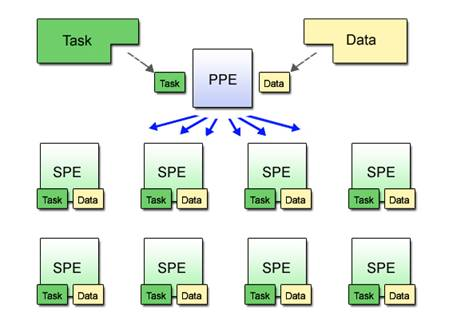
\includegraphics[width=.4\textwidth]{images/cell.jpg}
\end{center}
\hfill (from the Linux Cell documentation)

CUDA (Compute Unified Device Architecture) is NVIDIA's architecture
for processing on GPUs. ``C for CUDA'' predates OpenCL; NVIDIA still
makes CUDA tools available, and they may be faster than OpenCL on NVIDIA
hardware. On recent devices, you can use (most) C++ features in CUDA code,
which you can't do in OpenCL code.

OpenCL is a cross-vendor standard for GPU programming, and you can run
OpenCL programs on NVIDIA and AMD chips, as well as on CPUs. We will talk
about OpenCL for now.

\paragraph{Programming Model.} The programming
model for all of these architectures is similar: write the code for
the massively parallel computation (kernel) separately from the main
code, transfer the data to the GPU coprocessor (or execute it on the
CPU), wait, then transfer the results back.

OpenCL includes both task parallelism and data parallelism, as we've
discussed earlier in this course. \emph{Data parallelism} is central to
OpenCL; in OpenCL's view, you are evaluating a function, or \emph{kernel},
at a set of points, like so:

\begin{center}

\begin{tikzpicture}
\foreach \x in {0,0.25,...,2}
  \foreach \y in {0,0.25,...,2}
    \draw (\x, \y) circle (0.25mm);
\end{tikzpicture}
\end{center}

Another name for the set of points is the \emph{index space}. 
Each of the points corresponds to a \emph{work-item}.

OpenCL also supports \emph{task parallelism}: it can run different
kernels in parallel. Such kernels may have a one-point index space.
The documentation doesn't say much about task parallelism.

\paragraph{More on work-items.} The work-item is the fundamental
unit of work in OpenCL. These work-items live on an $n$-dimensional
grid (ND-Range); we've seen a 2-dimensional grid above. You may choose
to divide the ND-Range into smaller work-groups, or the system can
divide the range for you. OpenCL spawns a thread for each work item,
with a unique thread ID. The system runs each work-group on a set of
cores; NVIDIA calls that set a \emph{warp}, while ATI calls it a
\emph{wavefront}. The scheduler assigns work-items to the
warps/wavefronts until there are no more work items left.

\paragraph{Shared memory.} OpenCL makes lots of different types of
memory available to you:

\begin{itemize}
\item private memory: available to a single work-item;
\item local memory (aka ``shared memory''): shared between work-items
  belonging to the same work-group; like a user-managed cache;
\item global memory: shared between all work-items as well as the host;
\item constant memory: resides on the GPU, and cached. Does not change.
\end{itemize}

There is also host memory, which generally contains the application's
data.

\paragraph{An example kernel.} Let's continue by looking at 
a sample kernel, first written traditionally and then written
as an OpenCL kernel~\cite{khronos}.

{\scriptsize \hspace*{2em} \begin{minipage}{.8\textwidth} \begin{lstlisting}verbatim
  void traditional_mul(int n, const float *a, const float *b, float *c) {
    int i;
    for (i = 0; i < n; i++) c[i] = a[i] * b[i];
  }
    \end{lstlisting}
  \end{minipage}
  }

The same code looks like this as a kernel:

{\scriptsize \hspace*{1em} \begin{minipage}{.8\textwidth} \begin{lstlisting}verbatim
  kernel void opencl_mul(global const float *a, global const float *b, global float *c) {
    int id = get_global_id(0);  // dimension 0
    c[id] = a[id] * b[id];
  }
    \end{lstlisting}
  \end{minipage}
}

You can write kernels in a variant of C. OpenCL takes away some features,
like function pointers, recursion, variable-length arrays, bit fields,
and standard headers; and adds work-items, workgroups, vectors,
synchronization, and declarations of memory type. OpenCL also provides
a library for kernels to use.

\paragraph{Branches.} OpenCL implements a SIMT architecture.
What this means is that the computation for each work-item can branch
arbitrarily. The hardware will execute all branches that any thread in
a warp executed (which can be slow). 

{\scriptsize \hspace*{2em} \begin{minipage}{.5\textwidth}
    \begin{lstlisting}
kernel void contains_branch(global float *a, global float *b) {
    int id = get_global_id(0);
    if (cond) {
        a[id] += 5.0;
    } else {
        b[id] += 5.0;
    }
}
    \end{lstlisting}
      \end{minipage}}

In the above example, the {\tt if} statement will cause
each thread to execute both branches of the {\tt if}, keeping only the
result of the appropriate branch.

Similarly, executing a loop will cause the
workgroup to wait for the maximum number of iterations of the loop in
any work-item.

{\scriptsize \hspace*{2em} \begin{minipage}{.5\textwidth}
    \begin{lstlisting}verbatim
kernel void contains_loop(global float *a, 
                          global float *b) {
    int id = get_global_id(0);
    
    for (i = 0; i < id; i++) {
        b[i] += a[i];
    }
}
    \end{lstlisting}
\end{minipage} }

If you're setting up workgroups, though, you can arrange for all
of the work-items in a workgroup to execute the same branches.

\paragraph{Synchronization.} You might define
workgroups because you can only put barriers and memory fences between
work items in the same workgroup. Different workgroups execute
independently.

OpenCL also supports all of the notions that we've talked about
before: memory fences (read and write), barriers, and the volatile
keyword.  The barrier ({\tt barrier()}) ensures that all of the
threads in the workgroup all reach the barrier before they continue.
Recall that the fence ensures that no load or store instructions
(depending on the type of fence) migrate to the other side of the fence.

\section*{Complete OpenCL Example}
{
\begin{lstlisting}verbatim
// Note by PL: don't use this example as a template; it uses the C bindings!
// Instead, use the C++ bindings as in the other example.
// source: pages 1-9 through 1-11, http://developer.amd.com/wordpress/media/2013/07/AMD_Accelerated_Parallel_Processing_OpenCL_Programming_Guide-rev-2.7.pdf

//
// Copyright (c) 2010 Advanced Micro Devices, Inc. All rights reserved.
//
// A minimalist OpenCL program.
#include <CL/cl.h>
#include <stdio.h>
#define NWITEMS 512

// A simple memset kernel
const char *source =
"__kernel void memset( __global uint *dst )                             \n"
"{                                                                      \n"
"   dst[get_global_id(0)] = get_global_id(0);                           \n"
"}                                                                      \n";

int main(int argc, char ** argv)
{
   // 1. Get a platform.
   cl_platform_id platform;
   clGetPlatformIDs( 1, &platform, NULL );

   // 2. Find a gpu device.
   cl_device_id device;
   clGetDeviceIDs( platform, CL_DEVICE_TYPE_GPU,
		   1,
		   &device,
		   NULL);

   // 3. Create a context and command queue on that device.
   cl_context context = clCreateContext( NULL,
					 1,
					 &device,
					 NULL, NULL, NULL);
   cl_command_queue queue = clCreateCommandQueue( context,
						  device,
						  0, NULL );
   // 4. Perform runtime source compilation, and obtain kernel entry point.
   cl_program program = clCreateProgramWithSource( context,
						   1,
						   &source,
						   NULL, NULL );
   clBuildProgram( program, 1, &device, NULL, NULL, NULL );
   cl_kernel kernel = clCreateKernel( program, "memset", NULL );
   // 5. Create a data buffer.
   cl_mem buffer = clCreateBuffer( context,
				   CL_MEM_WRITE_ONLY,
				   NWITEMS * sizeof(cl_uint),
				   NULL, NULL );
   // 6. Launch the kernel. Let OpenCL pick the local work size.
   size_t global_work_size = NWITEMS;
   clSetKernelArg(kernel, 0, sizeof(buffer), (void*) &buffer);
   clEnqueueNDRangeKernel( queue,
			   kernel,
			   1,       // dimensions
			   NULL,    // initial offsets
			   &global_work_size, // number of work-items
			   NULL,    // work-items per work-group
                           0, NULL, NULL);  // events
   clFinish( queue );
   // 7. Look at the results via synchronous buffer map.
   cl_uint *ptr;
   ptr = (cl_uint *) clEnqueueMapBuffer( queue,
					 buffer,
					 CL_TRUE,
					 CL_MAP_READ,
					 0,
					 NWITEMS * sizeof(cl_uint),
					 0, NULL, NULL, NULL );
   int i;
   for(i=0; i < NWITEMS; i++)
       printf("%d %d\n", i, ptr[i]);
   return 0;
}
\end{lstlisting}
}

\paragraph{Walk-through.} Let's look at all of the code in the example and
explain the terms. 1) First, we request an OpenCL \emph{platform}.
Platforms, also known as hosts, contain 2) OpenCL \emph{compute devices},
which may in turn contain multiple compute units. Note that we could
also request a CPU device in step 2, without changing the rest of the code.

Next, in step 3, we request an OpenCL \emph{context} (representing all
OpenCL state) and create a \emph{command-queue}. We will request that
OpenCL do work by telling it to run a kernel in the queue.

In step 4, we create an OpenCL \emph{program}. This is a confusing
term; an OpenCL program is what runs on the compute unit, and includes
kernels, functions, and declarations. Your application can contain
more than one OpenCL program. In this case, we create a program
from the C string {\tt source}, which contains the kernel
{\tt memset}. OpenCL can also create programs from binaries, which may be
in an intermediate representation, or already compiled for a particular
device. We get a pointer to the kernel in this step, as the return
value from {\tt clCreateKernel}.

There's one more step before launching the kernel; in step 5, we
create a \emph{data buffer}, which enables communication between
devices. Recall that OpenCL requires explicit communication,
which we'll see later. Since this example doesn't have input, we 
don't need to put anything into the buffer initially.

Finally, we can launch the kernel in step 6. In this case, we don't
specify anything about workgroups, but enqueue the entire
1-dimensional index space, starting at $(0)$. We also state that the
index space has {\tt NWITEMS} elements, and not to subdivide the
problem into work-items. The last three parameters are about events.
We call {\tt clFinish()} to wait for the command-queue to empty.

Finally, in step 7, we copy the results back from the shared buffer
using {\tt clEnqueueMapBuffer}. This copy is blocking (first {\tt
  CL\_TRUE} argument), so we don't need an explicit {\tt clFinish()}
call. We also indicate the details of the command we'd like to
run: in particular, a read of {\tt NWITEMS} from the buffer.

You might also want to consider cleaning up the objects you've
allocated; I haven't shown that here. The code also doesn't contain
any error-handling.

It's important to note that this is a large amount of setup and accordingly overhead cost. Doing the setup, copying the data in, waiting, and copying the data out, all take time. But the GPU can do lots of work in parallel once it gets going. This is a lot like deciding whether to drive or fly. 

If the distance is short, say, 200 km (the distance between Ottawa and Montreal) then flying makes no sense: you have to get to the airport, be there at least an hour or two early to make your way through security checkpoints, then fly, then get from the destination airport to your final destination. Sure, the flying part is fast, but the overhead makes your total average speed not worth it.

On the other hand, if you're going a longer distance, like 4000 km (roughly the distance between Waterloo and San Francisco), then driving is way slower! Sure, the overhead of going the airport remains, but once you're in the air you're moving at 800 km/h or so and in 5.5 hours you are there. Compare that to 40 hours of driving.

\paragraph{C++ Bindings.}
    If we use the C++ bindings, we'll get automatic resource release and
      exceptions.
 C++ likes to use the RAII style
          (resource allocation is initialization).

\begin{itemize}
\item    Change the header to {\tt CL/cl.hpp} and define
      {\tt \_\_CL\_ENABLE\_EXCEPTIONS}.
\end{itemize}

We'd also like to store our kernel in a file instead of a string.
The C API is not so nice to work with; the C++ API is nicer. Use it!
As an example, you'll find the {\tt vector\_add} example in the slides and
in the code repo. 


\section*{More Complicated Kernel}
I've omitted the C code. it's pretty similar to what we saw
before, but it uses workgroups, customized to the number of
compute units on the device.  Here is a more interesting kernel, also from the same source.

{
\begin{lstlisting}verbatim
#pragma OPENCL EXTENSION cl_khr_local_int32_extended_atomics : enable
#pragma OPENCL EXTENSION cl_khr_global_int32_extended_atomics : enable
                                                                    
// 9. The source buffer is accessed as 4-vectors.                  
__kernel void minp( __global uint4 *src,                            
                    __global uint  *gmin,
                    __local uint   *lmin,                             
                    __global uint  *dbg,                             
                    size_t          nitems,                          
                    uint            dev )                            
{                                                                   
  // 10. Set up __global memory access pattern.                    
  uint count  = ( nitems / 4 ) / get_global_size(0);                
  uint idx    = (dev == 0) ? get_global_id(0) * count             
                           : get_global_id(0);                    
  uint stride = (dev == 0) ? 1 : get_global_size(0);               
  uint pmin   = (uint) -1;                                        
                                                                    
  // 11. First, compute private min, for this work-item.           
  for( int n=0; n < count; n++, idx += stride )                    
  {                                                                
    pmin = min( pmin, src[idx].x );                               
    pmin = min( pmin, src[idx].y );                               
    pmin = min( pmin, src[idx].z );                               
    pmin = min( pmin, src[idx].w );                               
  }                                                                
                                                                    
  // 12. Reduce min values inside work-group.                      
  if( get_local_id(0) == 0 )                                       
    lmin[0] = (uint) -1;                                          
  barrier( CLK_LOCAL_MEM_FENCE );                                  

  (void) atom_min( lmin, pmin );                                   
  barrier( CLK_LOCAL_MEM_FENCE );                                  
                                                                    
  // Write out to __global.                                        
  if( get_local_id(0) == 0 )                                       
    gmin[ get_group_id(0) ] = lmin[0];                            
                                                               
  // Dump some debug information.                             
  if( get_global_id(0) == 0 )
     { dbg[0] = get_num_groups(0); dbg[1] = get_global_size(0); 
       dbg[2] = count; dbg[3] = stride; }
}
                                                               
// 13. Reduce work-group min values from __global to __global. 
__kernel void reduce( __global uint4 *src, __global uint *gmin )                    
{                                                              
   (void) atom_min( gmin, gmin[get_global_id(0)] ) ;           
}                                                              
\end{lstlisting}
}

Let's discuss the notable features of this code, which finds the
minimum value from an array of 32-bit ints. (OpenCL ints are always 32
bits). Steps 1 through 8 are in the C code, which I've omitted; see
the AMD guide for the code. At 9), we can investigate the signature of
the {\tt minp} kernel. The use of {\tt uint4}, or 4-int vectors,
enables SSE instructions on CPUs and helps out GPUs as well. We'll
access the constituent {\tt int}s of {\tt src} using the {\tt .x},
{\tt .y}, {\tt .z} and {\tt .w} fields.  This kernel also writes to an
array of global minima, {\tt gmin}, and an array of local minima
(inside the workgroup), {\tt lmin}.

In step 10, we figure out where our point in the index space, as
reported by {\tt get\_global\_id()}, is located in the {\tt src}
index, as well as the stride, which is 1 for CPUs and $7 \times 64
\times c$, where $c$ is the number of work units, which was rounded up
using the following heuristic:

{
\begin{lstlisting}verbatim
  cl_uint ws = 64;
  global_work_size = compute_units * 7 * ws; // 7 wavefronts per SIMD
  while ( (num_src_items / 4) % global_work_size != 0 )
    global_work_size += ws;

  local_work_size = ws;
\end{lstlisting}
}


The core of the kernel occurs in step 11, where the {\tt for}-loop
computes the local minimum of the array elements in the work-item.  In
this stage, we are reading from the {\tt \_\_global} array {\tt src},
and writing to the private memory {\tt pmin}. This takes almost all of
the bandwidth. 

Then, in stage 12, thread 0 of the workgroup initializes the
workgroup-local {\tt lmin} value, and each thread atomically compares
(using the extended atomic requested using the pragma) its {\tt pmin}
to the local {\tt lmin} value.  We have local memory fences here to
make sure that threads stay in synch.  This code is not going to
consume much memory bandwidth, since there aren't many threads per
work-group, and there's only local communication.

Finally, thread 0 of the workgroup writes the local minimum of the
workgroup to the global array {\tt gmin}. In step 13, a second kernel
traverses the {\tt gmin} array and finds the smallest minimum.

\paragraph{Summary.} We've now seen the basics of GPU programming.
The key idea is to define a kernel and find a suitable index space.
Then you execute the kernel over the index space and collect results.
The main difficulty is in formulating your problem in such a way that
you can parallelize it, and then in splitting it into workgroups.


\section*{C++ Bindings Example}
Use the C++ bindings. They're better.

\begin{lstlisting}
// Vector add example, C++ bindings (use these!)
// source:
//  http://www.thebigblob.com/getting-started-
//        with-opencl-and-gpu-computing/

#define __CL_ENABLE_EXCEPTIONS

#include <CL/cl.hpp>

#include <iostream>
#include <fstream>
#include <string>
#include <utility>
#include <vector>
 
int main() {
    // Create the two input vectors
    const int LIST_SIZE = 1000;
    int *A = new int[LIST_SIZE]; 
    int *B = new int[LIST_SIZE];
    for(int i = 0; i < LIST_SIZE; i++) {
        A[i] = i;
        B[i] = LIST_SIZE - i;
    }

    try { 
        // Get available platforms
        std::vector<cl::Platform> platforms;
        cl::Platform::get(&platforms);

        // Select the default platform and create a context
        // using this platform and the GPU
        cl_context_properties cps[3] = { 
            CL_CONTEXT_PLATFORM, 
            (cl_context_properties)(platforms[0])(), 
            0 
        };
        cl::Context context(CL_DEVICE_TYPE_GPU, cps);
 
        // Get a list of devices on this platform
        std::vector<cl::Device> devices =
            context.getInfo<CL_CONTEXT_DEVICES>();
 
        // Create a command queue and use the first device
        cl::CommandQueue queue = cl::CommandQueue(context,
            devices[0]);

        // Read source file
        std::ifstream sourceFile("vector_add_kernel.cl");
        std::string sourceCode(
            std::istreambuf_iterator<char>(sourceFile),
            (std::istreambuf_iterator<char>())
        );
        cl::Program::Sources source(
            1,
            std::make_pair(sourceCode.c_str(),
                           sourceCode.length()+1)
        );
 
        // Make program of the source code in the context
        cl::Program program = cl::Program(context, source);
 
        // Build program for these specific devices
        program.build(devices);
 
        // Make kernel
        cl::Kernel kernel(program, "vector_add");
        
        // Create memory buffers
        cl::Buffer bufferA = cl::Buffer(
            context,
            CL_MEM_READ_ONLY,
            LIST_SIZE * sizeof(int)
        );
        cl::Buffer bufferB = cl::Buffer(
            context,
            CL_MEM_READ_ONLY,
            LIST_SIZE * sizeof(int)
        );
        cl::Buffer bufferC = cl::Buffer(
            context,
            CL_MEM_WRITE_ONLY,
            LIST_SIZE * sizeof(int)
        );
        
        // Copy lists A and B to the memory buffers
        queue.enqueueWriteBuffer(
            bufferA,
            CL_TRUE,
            0,
            LIST_SIZE * sizeof(int),
            A
        );
        queue.enqueueWriteBuffer(
            bufferB,
            CL_TRUE,
            0,
            LIST_SIZE * sizeof(int),
            B
        );
 
        // Set arguments to kernel
        kernel.setArg(0, bufferA);
        kernel.setArg(1, bufferB);
        kernel.setArg(2, bufferC);

        // Run the kernel on specific ND range
        cl::NDRange global(LIST_SIZE);
        cl::NDRange local(1);
        queue.enqueueNDRangeKernel(
            kernel,
            cl::NullRange,
            global,
            local
        );
 
        // Read buffer C into a local list
        int* C = new int[LIST_SIZE];
        queue.enqueueReadBuffer(
             bufferC,
             CL_TRUE,
             0,
             LIST_SIZE * sizeof(int),
             C
        );

        for(int i = 0; i < LIST_SIZE; i ++) {
            std::cout << A[i] << " + " << B[i] << " = "
                      << C[i] << std::endl;
        }
    } catch(cl::Error error) {
        std::cout << error.what() << "(" << error.err()
                  << ")" << std::endl;
    }
 
    return 0;
}
\end{lstlisting}









\chapter*{23 --- Password Cracking, Reduced-Resource Computation}

\addcontentsline{toc}{chapter}{23 --- Password Cracking, Reduced-Resource Computation}

\section*{GPU Application: Password Cracking}

GPUs are good---too good, even---at password cracking. We'll discuss a paper
that proposes a technique to make it harder to crack passwords. This technique
is scrypt, the algorithm behind DogeCoin~\cite{scrypt}. See also \url{http://www.tarsnap.com/scrypt.html}

First, let's talk about acceptable practices for password storage. It is \emph{not}
acceptable engineering practice to store passwords in plaintext. The inevitable security
breach will end with your company sending a ``sorry'' disclosure email to its clients,
and you will be responsible for the ensuing bad publicity.

Acceptable practices: {\bf not} plaintext; hashed and salted (we won't discuss salting here but hopefully you remember it from previous courses or other experience.)

\paragraph{Cryptographic hashing.} Instead of storing the plaintext password, you
store a hash of the password, under a cryptographic hash function. One important
property of a cryptographic hash function is that it must be (believed to be a) one-way
function; that is: $x \mapsto f(x)$, the forward direction, must be easy to compute, but
$f(x) \mapsto x$, the inverse mapping, must be hard to compute. Examples of such functions
include SHA1 and scrypt.

\paragraph{Not Secret.}
In real life, you can get around the idea of cryptographic hashing by looking on the internet to see if someone's password has already been leaked. Many services are terrible about their password storage policies so if you used the same username and password combination of mycrappywebsite.com and your online banking, then if the mycrappywebsite database gets hacked then the attacker has your user and password already without having to break anything.

\paragraph{First, Check if the Door Is Locked}
As you might imagine, the first thing to try is super common passwords: ``password'', ``system'', et cetera. Users frequently choose common words as passwords and if you just try them all you might get a hit. Choose stronger passwords!

\paragraph{Breaking the hash.} Even if there is no known short computation for the
inverse function, it's always possible to brute-force the password
computation by trying all possible passwords. Think about how GPUs
work. Each potential password is a point in the computation space, and
we compute the hash over all of them simultaneously.  That's a lot of
speedup. Custom hardware is also good, and those of you who know
something about hardware could think about implementing
it. Oh, hello, Bitcoin miners (but don't actually mine Bitcoin, please).

\paragraph{Arms race: making cracking difficult.} The idea has always been
to make it more difficult to compute the hash function, so that it's OK to
try one password, but it's intractable to try one billion passwords. Even way back,
UNIX passwords forced repeated applications of the hash function to accomplish these.

The main idea behind scrypt is to make hashing expensive in both time and space,
increasing both the number of operations and the cost of brute-forcing.
Hence crackers will need to use more circuitry to break passwords.

Of course, there's always this form of cracking:
\begin{center}
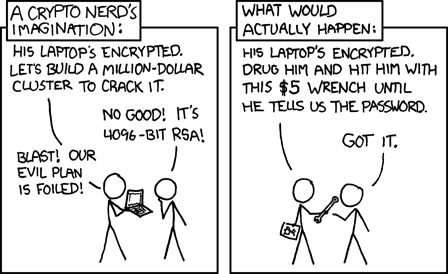
\includegraphics[width=0.5\textwidth]{images/xkcd-538}\\
\hfill (Source: xkcd 538)
\end{center}

\newtheorem{defn}{Definition}

\paragraph{Formalization.} Let's make the notion of ``expensive'' a bit more formal.
The idea is to force the use of the ``most memory possible'' for a given number of
operations. More memory implies more circuitry required to implement.

    \begin{defn}
      A \emph{memory-hard} algorithm on a Random Access Machine is an
      algorithm which uses $S(n)$ space and $T(n)$ operations, where
      $S(n) \in \Omega(T(n)^{1-\varepsilon})$.
    \end{defn}

Memory-hard algorithms are expensive to implement in either hardware or software.

Now, we want to move from particular algorithms to the underlying
functions (that is, we would like to quantify over all possible
algorithms). Intuitively, a \emph{sequential memory-hard function} is
one where (1) the fastest sequential algorithm is memory-hard; and (2)
it is impossible for a parallel algorithm to asymptotically achieve
lower cost.

\paragraph{Existence proof.} Of course anyone can define anything.
It's much better if the thing being defined actually exists. The
scrypt paper then goes on to exhibit ReMix, which is a concrete
example of a sequential memory hard function.

Finally, the paper concludes with an example of a more realistic
(cache-aware) model and a hard function in that context, BlockMix.

\paragraph{Rainbow Tables} So, the brute force approach is the simplest to describe but is computationally intensive, and if a sufficiently-well-designed cryptographic hash function is used it's really tough to actually crack a password. But maybe if we want to crack a password we don't have to always start from zero; maybe we could remember some previous computations so that we could use those answers later. If we calculated the hash of password ``12345'' and we knew what that looked like, if we encountered that hash in the future we could already jump immediately to the answer in our lookup table. This is the basic idea behind \textit{rainbow tables}.

There is a technical paper describing how rainbow tables work, but we'll instead use a much less cryptograhic-expert-level explanation~\cite{rainbowtables}. 

Part of the difficulty with this approach is that it isn't practical, or even really possible, to store the hashes for every possible plaintext (unless the plaintext is very small). So the rainbow table is a compromise between speed and space. The ``reduction'' function maps hashes to plaintext:

\begin{center}
	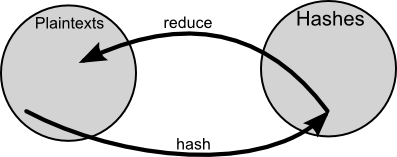
\includegraphics[width=0.4\textwidth]{images/rainbow-tables-reduce.png}\\
	Showing the reduce and hash functions~\cite{rainbowtables}.
\end{center}

This mapping function isn't the inverse of the hash function; it's just some sort of categorization. If the set of passwords to be cracked is, say, six digit numeric, then we compute the hash for a given input (``123456'') and we get some output (``d41d8cd98f00b204e9800998ecf8427e'') which is then reduced (mapped) to some other value (e.g., we'll take the first 6 numbers, 418980). We have another plaintext now, 418980. So we hash this new one, and reduce it, and so on and so on, until some end point ($n$ times, where you choose $n$). 

\begin{center}
	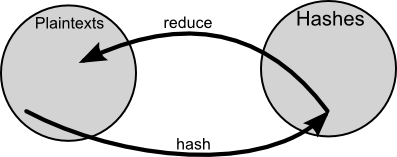
\includegraphics[width=0.4\textwidth]{images/rainbow-tables-reduce.png}\\
	And now we have a chain~\cite{rainbowtables}.
\end{center}

We should do this to develop some number of chains. This is the sort of task you could do with a GPU, because they can do a reduction relatively efficiently. 

Once we have those developed for a specific input set and hash function, they can be re-used forever. You do not even need to make them yourself anymore (if you don't want) because you can download them on the internet... they are not hard to find. They are large, yes, but in the 25 - 900 GB range, which is large  but not ridiculous. I mean, Fallout 76 had a day one patch of 52 GB, and it was a disaster of a game.

Alright, so, you've got them (or made them), but how do we use rainbow tables? Well, for a given hash with an unknown plaintext~\cite{rainbowtables}:
\begin{enumerate}
	\item Look for the hash in the list of final hashes; if there, we are done
	\item If it's not there, reduce the hash into another plaintext and hash the new plaintext
	\item Go back to step 1
	\item If the hash matches a final hash, the chain with the match contains the original hash
	\item Having identified the correct chain, we can start at the beginning of the chain with the starting plaintext and hash, check to see if we are successful (if so, we are done); if not, reduce and try the next plaintext. 
\end{enumerate} 

Like generation, checking the tables for a hit can also be done efficiently by the GPU. Some numbers from \url{http://www.cryptohaze.com/gpurainbowcracker.php.html}: 
\begin{itemize}
	\item Table generation on a GTX295 core for MD5 proceeds at around 430M links/sec.
	\item Cracking a password 'K\#n\&r4Z': real: 1m51.962s, user: 1m4.740s. sys: 0m15.320s
\end{itemize}

Yikes. There is obviously a little bit more complexity to how the rainbow tables work (such as dealing with collisions and loops), but it is clear just how devastatingly effective GPU computations are on breaking passwords.

\section*{The N-Body Problem and Reduced-Resource Computation}
A common physics problem that programmers are asked to simulate is the N-Body problem: you have some number of bodies (N!) and they interact via gravitational forces. The program needs to compute the movements of the bodies over time. This is a typical example of a program that is well suited to OpenCL: you can compute the forces on each body $n$ from all other bodies in parallel. This was even at one time an assignment in this course, although now there are too many good solutions on the internet so it was replaced. Ah well.

Once you've made the conversion to OpenCL and let's assume you've optimized it well so far. What can you do here if you want to speed it up even more? You could look for optimizations that trade off accuracy for performance. As you might imagine, using \texttt{float} instead of \texttt{double} can save half the space which should make things quite a bit faster. But you want more...

In the specific case of the N-body simulation,
domain knowledge would enable you to skimp out on
some unnecessary computation: points that are far away contribute only
very small forces. So you can estimate them (crudely). The idea is to divide the points into a number of ``bins'' which are cubes representing a locale of some sort. Then, compute the centre of mass for each bin. When calculating the forces on a given point, add the force exerted by the centre of mass for faraway bins to the force exerted by individual particles for nearby particles.

A more concrete explanation with an example: suppose the space  is divided into $[0, 1000]^3$, so we can take bins which are cubes of length 100. This gives 1000 bins. If you want to increase the accuracy, increase the number of bins. If you want to increase the speed, decrease the number of bins.

The program should have a 3-dimensional array {\tt cm} of {\tt
  float4}s to store centres-of-mass. The {\tt x}, {\tt y} and {\tt z}
components contain the average position of the centres of mass of a
bin, while the {\tt w} component stores the total mass. Compute all of
the masses in parallel: create one thread per bin, and add a point's
position if it belongs to the bin, e.g.

\begin{lstlisting}
    int xbin, ybin, zbin; // initialize with bin coordinates
    int b;
    for (i = 0; i < POINTS; i++) {
        if (pts[i] in bin coordinates) {
            cm[b].x += pts[i].x; // y, z too
            cm[b].w += 1.0f;
        }
    }
    cm[b].x /= cm[b].w; // etc
\end{lstlisting}

 \noindent
Note that this parallelizes with the number of bins.

For the next step, the program needs to keep track of the points in
each bin. Fortunately, you've collected the number of points in each
bin, so you can allocate the appropriate amount of memory to store the
points in a two-dimensional array {\tt binPts}. In a second phase,
iterate over all bins again, this time putting coordinates into the
proper element of {\tt binPts}.


The payoff from all these calculations is to save time while
calculating forces. In this example, we'll compute exact
forces for the points in the same bin and the directly-adjacent bins
in each direction (think of a Rubik's Cube; that makes 27 bins in all,
with 6 bins sharing a square, 12 bins sharing an edge, and 8 bins
sharing a point with the centre bin). If there is no adjacent bin 
(i.e., this is an edge), just act as if there are no points 
in the place where the nonexistent bin would be. 

Necessarily, writing the program like this is going to mean more than one kernel.
Each discrete step (compute centre of mass, put coordinates into bins, 
calculate forces) will be different kernels. This does mean there is overhead for each kernel, meaning the total amount of overhead goes up. Is it worth it? Let's see the data from a reference solution [PL] for the previous assignment:

\paragraph{With 500*64 points.}
\begin{itemize}
\item    OpenCL, no approximations (1 kernel): 0.182s
\item    OpenCL, with approximations (3 kernels): 0.168s
\end{itemize}
 \paragraph{With 5000*64 points.}
\begin{itemize}
\item    OpenCL, no approximations (1 kernel): 6.131s
\item    OpenCL, with approximations (3 kernels): 3.506s
\end{itemize}

\subsection*{Early phase termination}

In~\cite{Rinard:2010:PSA:1932682.1869525}, Martin Rinard summarizes
two of his novel ideas for automatic or semiautomatic optimizations
which trade accuracy for performance: early phase
termination~\cite{Rinard:2007:EarlyPhaseTermination} and loop
perforation~\cite{hoffmann09:_using_code_perfor_improv_perfor}. Both
of these ideas are applicable to code we've learned about in this
class.


We've talked about barriers quite a bit. Recall that the idea is that
no thread may proceed past a barrier until all of the threads
reach the barrier. Waiting for other threads causes delays. 
Killing slow threads obviously speeds up the program. Well, that's easy.

\begin{center}
``Oh no, that's going to change the meaning of the program!''
\end{center}

Let's consider some arguments about when it may be acceptable to just
kill (discard) tasks. Since we're not completely crazy, we can develop
a statistical model of the program behaviour, and make sure that the
tasks we kill don't introduce unacceptable distortions. Then when we
run the program, we get an output and a confidence interval.

\paragraph{Two Examples.} When might this work? Monte Carlo simulations
are a good candidate; you're already picking points randomly.
Raytracers can work as well. Both of these examples could spawn a lot
of threads and wait for all threads to complete.  In either case, you
can compensate for missing data points, assuming that they look like
the ones that you did compute. If you have a function where some graph is being
computed, you can probably guess that a missing point is somewhere in between
the two adjacent points.

The same is true for graphics, of course: if rendering a particular pixel did
not go well for some reason, you can just average the adjacent ones and probably
people would not notice the difference. Not bad!

Also recall that, in scientific computations, you're entering points
that were measured (with some error) and that you're computing
using machine numbers (also with some error). Computers are only
providing simulations, not the ground truth; the question is
whether the simulation is good enough.

\subsection*{Loop perforation} 
You can also apply the same idea to sequential programs. Instead
of discarding tasks, the idea here is to discard loop iterations.
Here's a simple example: instead of the loop,
\begin{center}
\verb|for (i = 0; i < n; i++) sum += numbers[i];|
\end{center} \vspace*{-1em}
simply write,
\vspace*{-1em}\begin{center}
\verb|for (i = 0; i < n; i += 2) sum += numbers[i];|
\end{center}
and multiply the end result by a factor of 2. This only works 
if the inputs are appropriately distributed, but it does give a
factor 2 speedup.

\paragraph{Example domains.} In~\cite{Rinard:2010:PSA:1932682.1869525},
we can read that loop perforation works for evaluating forces on water
molecules (in particular, summing numbers); Monte-Carlo simulation for
swaption pricing; and video encoding. In that example, changing loop
increments from 4 to 8 gives a speedup of 1.67, a signal to noise ratio
decrease of $0.87\%$, and a bitrate increase of $18.47\%$, producing
visually indistinguishable results. The computation looks like this:

{\small
\begin{verbatim}
min = DBL_MAX;
index = 0;
for (i = 0; i < m; i++) {
  sum = 0;
  for (j = 0; j < n; j++) sum += numbers[i][j];
  if (min < sum) {
    min = sum;
    index = i;
  }
}
\end{verbatim}
}
The optimization changes the loop increments and then compensates. 










\chapter*{24 --- Profiling}

\addcontentsline{toc}{chapter}{24 --- Profiling}

\section*{Profiling}

Think back to the beginning of the course when we did a quiz on what operations are fast and what operations are not. The important takeaway was not that we needed to focus on how to micro-optimize this abstraction or that hash function, but that our intuition about what is fast and what is slow is often wrong. Not just at a macro level, but at a micro level. You may be able to narrow down that this computation of $x$ is slow, but if you examine it carefully... what parts of it are slow?

If you don't use tools, then you end up guessing. You just make some assumptions about what you think is likely to be slow and try to change it. You've probably heard the famous quotation before, but here it is in its full form:

\begin{quote}
\textit{Programmers waste enormous amounts of time thinking about, or worrying about, the speed of noncritical parts of their programs, and these attempts at efficiency actually have a strong negative impact when debugging and maintenance are considered. We should forget about small efficiencies, say about 97\% of the time: premature optimization is the root of all evil. Yet we should not pass up our opportunities in that critical 3\%.}
\end{quote}
	\hfill -- Donald Knuth

So going about this blindly is probably a waste of time. You might be fortunate and optimize a slow part\footnote{There is a saying that even a blind squirrel sometimes finds a nut.} but we should really follow one of my favourite rules: ``don't guess, measure!''\footnote{Now I am certain you are sick of hearing that.} So, to make your programs or systems fast, you need to find out what is currently slow and improve it (duh!). Up until now in the course it's mostly been about ``let's speed this up'', but we did not take much time to decide what we should speed up (though you maybe did this on your assignment 2...?).

The general idea is, collect some data on what parts of the code are taking up the majority of the time. This can be broken down into looking at what functions get called, or how long functions take, or what's using memory...

There is always the ``informal'' way of doing this; it sort of works but it's not exactly the best plan. You probably know that when developing a program you can ``debug'' it without using any tools (e.g., \texttt{gdb}) by inserting a lot of print statements to the console or the log file. So when you enter function \texttt{foo} you print a nice little line on the console that say something like ``entering function foo'', associated with a timestamp and then when you're ready to return, a corresponding print function that says ``exiting'' appears, also with a timestamp.

This approach kind of works, and I've used it myself to figure out what blocks of a single large function are taking a long time (updating exchange rates... yeah). But this approach is not necessarily a good one.  It's an example of ``invasive'' profiling -- we are going in and changing the source code of the program in question -- to add instrumentation (log/debug statements). Plus we have to do a lot of manual accounting. Assuming your program is fast and goes through functions quickly and often, trying to put the pieces together manually is hopeless. It worked in that one example because the single function itself was running in the half hour range and I could see that the save operation was taking twelve minutes. Not kidding. 

(Also like debugging, if you get to be a wizard you can maybe do it by code inspection, but that technique of speculative execution inside your head is a lot harder to apply to performance problems than it is to debugging.)

So we should all agree, we want to use tools and do this in a methodical way.

Now that we agree on that, let's think about how profiling tools work\:

\begin{itemize}
\item sampling-based (traditional): every so often (e.g. 100ms for gprof), query the
system state; or,
\item instrumentation-based, or probe-based/predicate-based
  (traditionally too expensive): query system state under certain
  conditions; like conditional breakpoints.
\end{itemize}
We'll talk about both per-process profiling and system-wide profiling.

If you need your system to run fast, you need to start profiling
and benchmarking as soon as you can run the system. Benefits:
\begin{itemize}
\item establishes a baseline performance for the system;
\item allows you to measure impacts of changes and further system development;
\item allows you to re-design the system before it's too late;
\item avoids the need for ``perf spray'' to make the system faster, since
that spray is often made of ``unobtainium''\footnote{\url{http://en.wikipedia.org/wiki/Unobtainium}}.
\end{itemize}

\paragraph{Tips for Leveraging Profiling.}
When writing large software projects:
  \begin{itemize}
    \item First, write clear and concise code. \\
      Don't do any premature optimizations---focus on correctness.
    \item Profile to get a baseline of your performance:
      \begin{itemize}
        \item allows you to easily track any performance changes;
        \item allows you to re-design your program before it's too late.
      \end{itemize}
  \end{itemize}
Focus your optimization efforts on the code that matters.

Look for abnormalities; in particular, you're looking for
deviations from the following rules:
\begin{itemize}
\item time is spent in the right part of the system/program;
\item time is not spent in error-handling, noncritical code, or exceptional cases; and
\item time is not unnecessarily spent in the operating system.
\end{itemize}
For instance, ``why is {\tt ps} taking up all my cycles?'';
see page 34 of ~\cite{300ps}.

\paragraph{Development vs. production.}
You can always profile your systems in development, but that might not
help with complexities in production. (You want separate dev and
production systems, of course!) We'll talk a bit about DTrace, which
is one way of profiling a production system. The constraints on profiling 
production systems are that the profiling must not affect the system's
performance or reliability.

\section*{Userspace per-process profiling}
Sometimes---or, in this course, often---you can get away with
investigating just one process and get useful results about that
process's behaviour.  We'll first talk about {\tt gprof}, the GNU
profiler
tool\footnote{\url{http://sourceware.org/binutils/docs/gprof/}}, and
then continue with other tools.

{\tt gprof} does sampling-based profiling for single processes: it
requests that the operating system interrupt the process being
profiled at regular time intervals and figures out which procedure is
currently running. It also adds a bit of instrumentation to collect
information about which procedures call other procedures.

\paragraph{``Flat'' profile.} The obvious thing to do with the
profile information is to just print it out. You get a list of
procedures called and the amount of time spent in each of these 
procedures.

The general limitation is that procedures that don't run for
long enough won't show up in the profile. (There's a caveat: if
the function was compiled for profiling, then it will show up
anyway, but you won't find out about how long it executed for).

\paragraph{``Call graph''.} {\tt gprof} can also print out 
its version of a call graph, which shows the amount of time that
either a function runs (as in the ``flat'' profile) as well as the
amount of time that the callees of the function run.  Another term for
such a call graph is a ``dynamic call graph'', since it tracks the
dynamic behaviour of the program.  Using the {\tt gprof} call graph,
you can find out who is responsible for calling the functions that
take a long time.

\paragraph{Limitations of {\tt gprof}.} Beyond the usual limitations
of a process-oriented profiler, {\tt gprof} also suffers limitations
from running completely in user-space. That is, it has no access to
information about system calls, including time spent doing I/O.
It also doesn't know anything about the CPU's built-in counters
(e.g. cache miss counts, etc). Like the other profilers, it causes
overhead when it's running, but the overhead isn't too large.

\section*{{\tt gprof} usage guide}
We'll give some details about using {\tt gprof}. First,
use the {\tt -pg} flag with {\tt clang} when compiling and linking.
(It's currently broken in gcc, unless you give {\tt -no-pie}.)
Next, run your program as you normally would.
 Your program will now create {\tt gmon.out}.

Use gprof to interpret the results: {\tt gprof <executable>}.

\paragraph*{Example.} Consider a program with 100 million calls 
to two math functions.

\begin{tabular}{ll}
\begin{minipage}{.5\textwidth}
\begin{lstlisting}[language=C,basicstyle=\scriptsize]
int main() {
    int i,x1=10,y1=3,r1=0;
    float x2=10,y2=3,r2=0;

    for(i=0;i<100000000;i++) {
        r1 += int_math(x1,y1);
        r2 += float_math(y2,y2);
    }
}

int int_math(int x, int y){
    int r1;
    r1=int_power(x,y);
    r1=int_math_helper(x,y);
    return r1;
}

int int_math_helper(int x, int y){
    int r1;
    r1=x/y*int_power(y,x)/int_power(x,y);
    return r1;
}

int int_power(int x, int y){
    int i, r;
    r=x;
    for(i=1;i<y;i++){
        r=r*x;
    }
    return r;
}
\end{lstlisting}
\end{minipage}
\begin{minipage}{0.5\textwidth}
\begin{lstlisting}[language=C]
float float_math(float x, float y) {
    float r1;
    r1=float_power(x,y);
    r1=float_math_helper(x,y);
    return r1;
}

float float_math_helper(float x, float y) {
    float r1;
    r1=x/y*float_power(y,x)/float_power(x,y);
    return r1;
}

float float_power(float x, float y){
    float i, r;
    r=x;
    for(i=1;i<y;i++) {
        r=r*x;
    }
    return r;
}
  \end{lstlisting}
\end{minipage}
\end{tabular}

Looking at the code, we have no idea what takes longer.
One might guess that floating point math takes longer. This is admittedly a
silly example, but it works well to illustrate our point.

\paragraph{Flat Profile Example.}
    When we run the program and look at the flat profile, we see:

  \begin{lstlisting}
          Flat profile:

          Each sample counts as 0.01 seconds.
            %   cumulative   self              self     total           
           time   seconds   seconds    calls  ns/call  ns/call  name    
           32.58      4.69     4.69 300000000    15.64    15.64  int_power
           30.55      9.09     4.40 300000000    14.66    14.66  float_power
           16.95     11.53     2.44 100000000    24.41    55.68  int_math_helper
           11.43     13.18     1.65 100000000    16.46    45.78  float_math_helper
            4.05     13.76     0.58 100000000     5.84    77.16  int_math
            3.01     14.19     0.43 100000000     4.33    64.78  float_math
            2.10     14.50     0.30                             main
  \end{lstlisting}

 There is one function per line. Here are what the columns mean:
  \begin{itemize}
    \item {\bf \% time:} the percent of the total execution time in this function.
    \item {\bf self:} seconds in this function.
    \item {\bf cumulative:} sum of this function's time + any above it in table.
    \item {\bf calls:} number of times this function was called.
    \item {\bf self ns/call:} just self nanoseconds / calls.
    \item {\bf total ns/call:} mean function execution time, including
       calls the function makes.
  \end{itemize}

\paragraph{Call Graph Example.}
After the flat profile gives you a feel for which functions are costly, you
      can get a better story from the call graph.

  \begin{lstlisting}
          index % time    self  children    called     name
                                                           <spontaneous>
          [1]    100.0    0.30   14.19                 main [1]
                          0.58    7.13 100000000/100000000     int_math [2]
                          0.43    6.04 100000000/100000000     float_math [3]
          -----------------------------------------------
                          0.58    7.13 100000000/100000000     main [1]
          [2]     53.2    0.58    7.13 100000000         int_math [2]
                          2.44    3.13 100000000/100000000     int_math_helper [4]
                          1.56    0.00 100000000/300000000     int_power [5]
          -----------------------------------------------
                          0.43    6.04 100000000/100000000     main [1]
          [3]     44.7    0.43    6.04 100000000         float_math [3]
                          1.65    2.93 100000000/100000000     float_math_helper [6]
                          1.47    0.00 100000000/300000000     float_power [7]
          -----------------------------------------------
                          2.44    3.13 100000000/100000000     int_math [2]
          [4]     38.4    2.44    3.13 100000000         int_math_helper [4]
                          3.13    0.00 200000000/300000000     int_power [5]
          -----------------------------------------------
                          1.56    0.00 100000000/300000000     int_math [2]
                          3.13    0.00 200000000/300000000     int_math_helper [4]
          [5]     32.4    4.69    0.00 300000000         int_power [5]
          -----------------------------------------------
                          1.65    2.93 100000000/100000000     float_math [3]
          [6]     31.6    1.65    2.93 100000000         float_math_helper [6]
                          2.93    0.00 200000000/300000000     float_power [7]
          -----------------------------------------------
                          1.47    0.00 100000000/300000000     float_math [3]
                          2.93    0.00 200000000/300000000     float_math_helper [6]
          [7]     30.3    4.40    0.00 300000000         float_power [7]
  \end{lstlisting}

To interpret the call graph, note that the line with the index [N] is the \emph{primary line},
or the current function being considered.
\begin{itemize}
    \item Lines above the primary line are the functions which called this function.
    \item Lines below the primary line are the functions which were called by this function
      (children).
\end{itemize}

For the primary line, the columns mean:
  \begin{itemize}  
    \item {\bf time:} total percentage of time spent in this function and its
      children.
    \item {\bf self:} same as in flat profile.
    \item {\bf children:} time spent in all calls made by the function;
      \begin{itemize}
        \item should be equal to self + children of all functions below.
      \end{itemize}
  \end{itemize}

For callers (functions above the primary line):
  \begin{itemize}
    \item {\bf self:} time spent in primary function, when called from current
      function.
    \item {\bf children:} time spent in primary function's children, when
      called from current function.
    \item {\bf called:} number of times primary function was called from current
      function / number of nonrecursive calls to primary function.
  \end{itemize}

For callees (functions below the primary line):
  \begin{itemize}  
    \item {\bf self:} time spent in current function when called from primary.
    \item {\bf children:} time spent in current function's children calls when
      called from primary.
      \begin{itemize}
        \item self + children is an estimate of time spent in current function
          when called from primary function.
      \end{itemize}
    \item {\bf called:} number of times current function was called from primary
      function / number of nonrecursive calls to current function.
  \end{itemize}

Based on this information, we can now see where most of the time comes
from, and pinpoint any locations that make unexpected calls, etc.
This example isn't too exciting; we could simplify the math and optimize the
program that way.









\chapter*{25 --- Using Google Performance Tools}

\addcontentsline{toc}{chapter}{25 --- Using Google Performance Tools}

\section*{Introduction to gperftools}
Next, we'll talk about the Google Performance Tools. 
\begin{center}
\url{http://google-perftools.googlecode.com/svn/trunk/doc/cpuprofile.html}
\end{center}
They include:
      \begin{itemize}
        \item a CPU profiler
        \item a heap profiler
        \item a heap checker; and 
        \item a faster (multithreaded) {\tt malloc}.
      \end{itemize}

We'll mostly use the CPU profiler. Characteristics include:
      \begin{itemize}
        \item  supposedly works for
multithreaded programs;
        \item purely statistical sampling;
        \item no recompilation required (typically benefit from re-linking); and
        \item better output, including built-in graphical output.
      \end{itemize}

You can use the profiler without any recompilation. But this is not recommended;
you'll get worse data. Use {\tt LD\_PRELOAD}, which changes the dynamic libraries that
an executable uses.

  \begin{lstlisting}[basicstyle=\scriptsize]
  % LD_PRELOAD="/usr/lib/libprofiler.so" CPUPROFILE=test.prof ./test
  \end{lstlisting}

The other (more-recommended) option is to link to the profiler with {\tt -lprofiler}.

Both options read the {\tt CPUPROFILE} environment variable, which
specifies where profiling data goes.

You can use the profiling library directly as well:
\begin{lstlisting}[basicstyle=\scriptsize]
          #include <gperftools/profiler.h>
\end{lstlisting}
Then, bracket code you want profiled with:
\begin{lstlisting}[basicstyle=\scriptsize]
          ProfilerStart()
          // ...
          ProfilerStop()
\end{lstlisting}
    
You can change the sampling frequency with the {\tt CPUPROFILE\_FREQUENCY} environment variable
(default value 100 interrupts/second).

\paragraph{{\tt pprof} usage.} {\tt pprof} is like {\tt gprof} for Google Perf Tools. It
analyzes profiling results. Here are some usage examples.
  \begin{lstlisting}[basicstyle=\scriptsize]
          % pprof test test.prof
              Enters "interactive" mode
          % pprof --text test test.prof
              Outputs one line per procedure
          % pprof --gv test test.prof
               Displays annotated call-graph via 'gv'
          % pprof --gv --focus=Mutex test test.prof
              Restricts to code paths including a .*Mutex.* entry
          % pprof --gv --focus=Mutex --ignore=string test test.prof
              Code paths including Mutex but not string
          % pprof --list=getdir test test.prof
              (Per-line) annotated source listing for getdir()
          % pprof --disasm=getdir test test.prof
              (Per-PC) annotated disassembly for getdir()
  \end{lstlisting}

Can also output {\tt dot}, {\tt ps}, {\tt pdf} or {\tt gif} instead of {\tt gv}.

\paragraph{{\tt gprof} text output.}
This is similar to the flat profile in {\tt gprof}.

  \begin{lstlisting}[basicstyle=\scriptsize]
          jon@riker examples master % pprof --text test test.prof 
          Using local file test.
          Using local file test.prof.
          Removing killpg from all stack traces.
          Total: 300 samples
                95  31.7%  31.7%      102  34.0% int_power
                58  19.3%  51.0%       58  19.3% float_power
                51  17.0%  68.0%       96  32.0% float_math_helper
                50  16.7%  84.7%      137  45.7% int_math_helper
                18   6.0%  90.7%      131  43.7% float_math
                14   4.7%  95.3%      159  53.0% int_math
                14   4.7% 100.0%      300 100.0% main
                 0   0.0% 100.0%      300 100.0% __libc_start_main
                 0   0.0% 100.0%      300 100.0% _start
  \end{lstlisting}

Columns, from left to right, denote:
\begin{itemize}
\item  Number of samples in this function.
\item  Percentage of samples in this function (same as {\bf time} in {\tt gprof}).
\item  Percentage of checks in the functions printed so far (equivalent to {\bf cumulative}, but in \%).
\item     Number of checks in this function and its callees.
\item     Percentage of checks in this function and its callees.
\item    Function name.
\end{itemize}

\paragraph{Graphical Output.} Google Perf Tools can also produce graphical output:

\begin{center}
    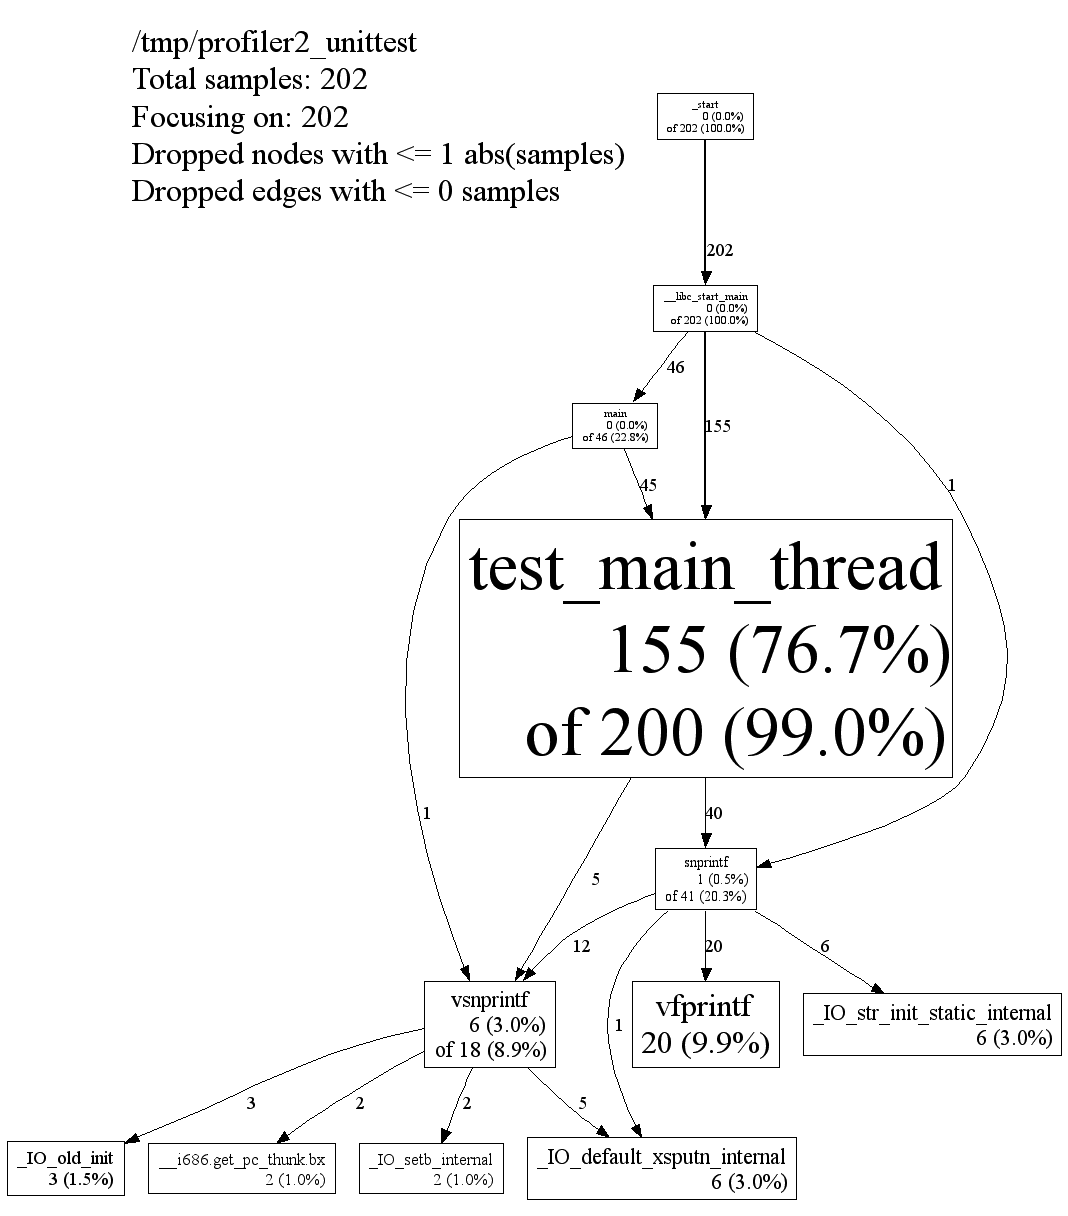
\includegraphics[scale=0.3]{images/pprof-test-big.png}
\end{center}

This shows the same numbers as the text output. This particular graphical example is on a different program than the text output, and that's why they look different. Directed edges denote function calls.
Note: 
\[ \mbox{\# of samples in callees} = \mbox{\# in ``this function + callees''} - \mbox{\# in ``this function''}.\]

For example, in {\tt float\_math\_helper}, we have ``51 (local) of 96 (cumulative)''.
Here,
\[ 96 - 51 = 45 \mbox{ (callees)}. \]
      \begin{itemize}
        \item callee {\tt int\_power} = 7 (bogus)
        \item callee {\tt float\_power} = 38
        \item callees total = 45
      \end{itemize}

Note that the call graph is not exact.
In fact, it shows many bogus relations which clearly don't exist.
For instance, we know that there are no cross-calls between {\tt int} and {\tt float} functions.

As with {\tt gprof}, optimizations will change the
      graph.\

You'll probably want to look at the text profile first, then use the
      {\tt --focus} flag to look at individual functions.

      \section*{System-level profiling}
Most profiling tools interrogate the CPU in more detail than {\tt
  gprof} and friends. These tools are typically aware of the whole
system, but may focus on one application, and may have both
per-process and system-wide modes. We'll discuss a couple of these
tools here, highlighting conceptual differences between these
applications.

\paragraph{Solaris Studio Performance Analyzer.} This 
tool\footnote{You can find a high-level description at
  \url{http://www.oracle.com/technetwork/server-storage/solarisstudio/documentation/oss-performance-tools-183986.pdf}}
supports {\tt gprof}-style profiling (``clock-based profiling'') as
well as kernel-level profiling through DTrace (described later). At
process level, it collects more process-level data than {\tt gprof},
including page fault times and wait times. It also can read CPU
performance counters (e.g. the number of executed floating point adds
and multiplies).  As a Sun application, it also works with Java
programs.

Since locks and concurrency are important, modern tools, including the
Studio Performance Analyzer, can track the amount of time spent
waiting for locks, as well as statistics about MPI message
passing. More on lock waits below, when we talk about WAIT.

\paragraph{VTune.} Intel and AMD both provide profiling
tools; Intel's VTune tool costs money, while AMD's CodeAnalyst tool is
free software.

Intel uses the term ``event-based sampling'' to refer to sampling 
which fires after a certain number of CPU events occur, and ``time-based
sampling'' to refer to the {\tt gprof}-style sampling (e.g. every 100ms).
VTune can also correlate the behaviour of the counters with other
system events (like disk workload). Both of these sampling modes
also include the behaviour of the operating system and I/O in their
counts.

VTune also supports an instrumentation-based profiling approach,
which measures time spent in each procedure (same type of
data as {\tt gprof}, but using a different collection scheme).

VTune will also tell you what it thinks the top problems with your
software are. However, if you want to understand what it's saying,
you do actually need to understand the architecture.

\paragraph{CodeAnalyst.} AMD also provides a profiling tool. Unlike Intel's tool, AMD's tool is
free software (the Linux version is released under the GPL), so that,
for instance, Mozilla suggests that people include CodeAnalyst
profiling data when reporting Firefox performance
problems~\footnote{\url{https://developer.mozilla.org/Profiling_with_AMD_CodeAnalyst}}.

CodeAnalyst is a system-wide profiler. It supports drilling down into
particular programs and libraries; the only disadvantage of being
system-wide is that the process you're interested in has to execute
often enough to show up in the profile. It also uses debug symbols to
provide meaningful names; these symbols are potentially supplied over
the Internet.

Like all profilers, it includes a sampling mode, which it calls ``Time-based
profiling'' (TBP). This mode works on all processors. The other modes are 
``Event-based profiling'' (EBP) and ``Instruction-based sampling'' (IBS);
these modes use hardware performance counters.

AMD's CodeAnalyst documentation points out that your sampling interval
needs to be sufficiently high to capture useful data, and that you need to 
take samples for enough time. The default sampling rate is once every
millisecond, and they suggest that programs should run for at least 15 seconds
to get meaningful data.

The EBP mode works like VTune's event-based sampling: after a certain
number of CPU events occur, the profiler records the system state.
That way, it knows where e.g. all the cache misses are occuring.
A caveat, though, is that EBP can't exactly identify the guilty statement,
because of ``skid'': in the presence of out-of-order execution, guilt
gets spread to the adjacent instructions.

To improve the accuracy of the profile information, CodeAnalyst uses
AMD hardware features to watch specific x86 instructions and ``ops'',
their associated backend instructions. This is the IBS mode\footnote{Available
on AMD processors as of the K10 family---typically manufactured in 2007+; see \url{http://developer.amd.com/assets/AMD_IBS_paper_EN.pdf}. Thanks to Jonathan Thomas for pointing this out.} of
CodeAnalyst.  AMD provides an
example\footnote{\url{http://developer.amd.com/cpu/CodeAnalyst/assets/ISPASS2010_IBS_CA_abstract.pdf}}
where IBS tracks down the exact instruction responsible for data
translation lookaside buffer (DTLB) misses, while EBP indicates four
potential guilty instructions.


\paragraph{oprofile.} This free software is a sampling-based tool which uses the Linux Kernel Performance
Events API to access CPU performance counters. It tracks the
currently-running function (or even the line of code) and can, in
system-wide mode, work across processes, recording data for every
active application.

Webpage: \url{http://oprofile.sourceforge.net}.

You can run oprofile either in system-wide mode (as root) or per-process. To run it in system-wide mode:
  \begin{lstlisting}
% sudo opcontrol --vmlinux=/usr/src/linux-3.2.7-1-ARCH/vmlinux
% echo 0 | sudo tee /proc/sys/kernel/nmi_watchdog
% sudo opcontrol --start
Using default event: CPU_CLK_UNHALTED:100000:0:1:1
Using 2.6+ OProfile kernel interface.
Reading module info.
Using log file /var/lib/oprofile/samples/oprofiled.log
Daemon started.
Profiler running.
  \end{lstlisting}

Or, per-process:
\begin{lstlisting}
[plam@lynch nm-morph]$ operf ./test_harness
operf: Profiler started

Profiling done.
\end{lstlisting}%$

Both of these invocations produce profiling output. You can read the profiling output
by running {\tt opreport} and giving it your executable.

  \begin{lstlisting}
% sudo opreport -l ./test    
CPU: Intel Core/i7, speed 1595.78 MHz (estimated)
Counted CPU_CLK_UNHALTED events (Clock cycles when not
halted) with a unit mask of 0x00 (No unit mask) count 100000
samples  %        symbol name
7550     26.0749  int_math_helper
5982     20.6596  int_power
5859     20.2348  float_power
3605     12.4504  float_math
3198     11.0447  int_math
2601      8.9829  float_math_helper
160       0.5526  main
  \end{lstlisting}
  If you have debug symbols ({\tt -g}) you can also get better data:
  {\small
  \begin{lstlisting}
% sudo opannotate --source --output-dir=/path/to/annotated-source /path/to/mybinary
  \end{lstlisting}
  }

Use {\tt opreport} by itself for a whole-system view.
    You can also reset and stop the profiling.
  \begin{lstlisting}
% sudo opcontrol --reset 
Signalling daemon... done
% sudo opcontrol --stop
Stopping profiling.
  \end{lstlisting}

\paragraph{perf.} This uses the same base data as oprofile, but provides a better
(git-like) interface. Once again, it is an interface to the Linux kernel's built-in
sample-based profiling using CPU counters. It works per-process, per-CPU, or system-wide.
It can report the cost of each line of code.

Webpage: \url{https://perf.wiki.kernel.org/index.php/Tutorial}

\noindent
Here's a usage example on some old assignment code from last year:
\begin{lstlisting}[basicstyle=\scriptsize]
[plam@lynch nm-morph]$ perf stat ./test_harness

 Performance counter stats for './test_harness':

       6562.501429 task-clock                #    0.997 CPUs utilized          
               666 context-switches          #    0.101 K/sec                  
                 0 cpu-migrations            #    0.000 K/sec                  
             3,791 page-faults               #    0.578 K/sec                  
    24,874,267,078 cycles                    #    3.790 GHz                     [83.32%]
    12,565,457,337 stalled-cycles-frontend   #   50.52% frontend cycles idle    [83.31%]
     5,874,853,028 stalled-cycles-backend    #   23.62% backend  cycles idle    [66.63%]
    33,787,408,650 instructions              #    1.36  insns per cycle        
                                             #    0.37  stalled cycles per insn [83.32%]
     5,271,501,213 branches                  #  803.276 M/sec                   [83.38%]
       155,568,356 branch-misses             #    2.95% of all branches         [83.36%]

       6.580225847 seconds time elapsed
\end{lstlisting} %$

\noindent
perf can tell you which instructions are taking time, or which lines
of code; compile with {\tt -ggdb} to enable source code viewing.

\begin{lstlisting}
% perf record ./test_harness
% perf annotate
\end{lstlisting}

\noindent
{\tt perf annotate} is interactive. Play around with it.

\paragraph{DTrace.} 
DTrace~\cite{Cantrill:2004:DIP:1247415.1247417} is an instrumentation-based
system-wide profiling tool designed to be used on production
systems. It supports custom queries about system behaviour: when you
are debugging system performance, you can collect all sorts of data
about what the system is doing. The two primary design goals were in
support of use in production: 1) avoid overhead when not tracing and
2) guarantee safety (i.e. DTrace can never cause crashes).

DTrace runs on Solaris and some BSDs. There is a Linux port, which may be usable.
I'll try to install it on {\tt ece459-1}.

\paragraph{Probe effect.} ``Wait! Don't `instrumentation-based' 
and `production systems' not go together?'' For instance, Valgrind incurs a 100$\times$
slowdown. Ouch.

Nope! DTrace was designed to have zero overhead when inactive. It does
this by dynamically rewriting the code to insert instrumentation when
requested. So, if you want to instrument all calls to the {\tt open}
system call, then DTrace is going to replace the instruction at the
beginning of {\tt open} with an unconditional branch to the
instrumentation code, execute the profiling code, then return to your
code. Otherwise, the code runs exactly as if you weren't looking.

\paragraph{Safety.} As I've mentioned before, crashing a production
system is a big no-no. DTrace is therefore designed to never cause a
system crash. How? The instrumentation you write for DTrace 
must conform to fairly strict constraints.

\paragraph{DTrace system design.} The DTrace framework supports instrumentation
\emph{providers}, which make \emph{probes} (i.e.  instrumentation
points) available; and \emph{consumers}, which enable probes as
appropriate. Examples of probes include system calls, arbitrary kernel
functions, and locking actions. Typically, probes apply at function entry or exit points.
DTrace also supports typical
sampling-based profiling in the form of timer-based probes; that is,
it executes instrumentation every 100ms. This is tantamount to
sampling.

You can specify a DTrace clause using probes, predicates, and a set of
action statements. The action statements execute when the condition
specified by the probe holds and the predicate evaluates to true. D
programs consist of a sequence of clauses.

\paragraph{Example.} Here's an example of a DTrace query from~\cite{Cantrill:2004:DIP:1247415.1247417}.

{ \begin{verbatim}
    syscall::read:entry {
            self->t = timestamp;
    }

    syscall::read:return
    /self->t/ {
            printf("%d/%d spent %d nsecs in read\n"
                pid, tid, timestamp - self->t);
    }
    \end{verbatim}
}

The first clause instruments all entries to the system call {\tt read}
and sets a thread-local variable {\tt t} to the current time. The
second clause instruments returns from {\tt read} where the
thread-local variable {\tt t} is non-zero, calling {\tt printf} to print out
the relevant data.

The D (DTrace clause language) design ensures that clauses cannot loop indefinitely
(since they can't loop at all), nor can they execute unsafe code;
providers are responsible for providing safety guarantees. Probes
might be unsafe because they might interrupt the system at a critical
time. Or, action statements could perform illegal writes. DTrace won't 
execute unsafe code.

\paragraph{Workflow.} Both the USENIX article~\cite{Cantrill:2004:DIP:1247415.1247417} and the
ACM Queue article~\cite{300ps} referenced above contain example usages of DTrace.
In high-level terms: first identify a problem; then, use
standard system monitoring tools, plus custom DTrace queries,
to collect data about the problem (and resolve it).

\section*{WAIT}
Another approach which recently appeared in the research literature is
the WAIT tool out of IBM. Unfortunately, this tool is not free and not
generally available. Let's talk about it anyways.

Like DTrace, WAIT is suitable for use in production environments. It
uses hooks built into modern Java Virtual Machines (JVMs) to analyze
their idle time. It performs a sampling-based analysis of the
behaviour of the Java VM. Note that its samples are quite infrequent;
they suggest that taking samples once or twice a minute is enough.  At
each sample, WAIT records the state of each of the threads, which
includes its call stack and participation in system locks. This data
enables WAIT to compute (using expert rules) an abstract ``wait
state''.  The wait state indicates what the process is currently doing
or waiting on, e.g. ``disk'', ``GC'', ``network'', or ``blocked''.

\paragraph{Workflow.} You run your application, collect data (using a
script or manually), and upload the data to the server. The server provides
a report which you use to fix the performance problems.
The report indicates processor utilization (idle, your application, GC, 
etc); runnable threads; waiting threads (and why they are waiting); 
thread states; and a stack viewer.

The paper presents six case studies where WAIT helped solve performance
problems, including deadlocks, server underloads, memory leaks, database
bottlenecks, and excess filesystem activity.

\subsection*{Other Applications of Profiling.} 
Profiling applies to languages beyond C/C++ and Java, of course. If you are
profiling an interpreted language, you'll need a specific tool to get useful
results. For Python, you can use {\tt cProfile}; it is a standard implementation
of profiling, from what I can see.


Here's a short tangent. Many of the concepts that we've seen for code
also apply to web pages. Google's Page Speed
tool\footnote{\url{http://code.google.com/speed/page-speed/}}, in
conjunction with Firebug, helps profile web pages, and provides
suggestions on how to make your web pages faster. Note that Page Speed
includes improvements for the web page's design, e.g. not requiring
multiple DNS lookups; leveraging browser caching; or combining images;
as well as traditional profiling for the JavaScript on your pages.










\chapter*{26 --- Liar, Liar}

\addcontentsline{toc}{chapter}{26 --- Liar, Liar}

\section*{Lies about Calling Context}

Let's open with a video that illustrates one of the problems with sampling-based profiling:

\begin{center}
	\url{https://www.youtube.com/watch?v=jQDjJRYmeWg}
\end{center}

The video's not fake; it's a real helicopter and it's really flying. What's happening, however, is that the camera is taking images at some multiple of the frequency of the blade rotation speed so it gives the illusion that the blades are not spinning at all. This is a sampling problem, and you see the same problem in car commercials on TV where it looks like the wheels are spinning backwards. They're not, but the sampling effect of the camera can make it look that way.

Some profiler results are real.  Other results are interpolated, and
perhaps wrong. Who can we trust? We'll start by talking about gprof and callgrind/KCacheGrind. The reference for this part of the lecture is a blog post by Yossi Kreinin~\cite{lies}.

\paragraph{Running Example.} Consider the following code.

\begin{lstlisting}
void work(int n) {
  volatile int i=0; //don't optimize away
  while(i++ < n);
}
void easy() { work(1000); }
void hard() { work(1000*1000*1000); }
int main() { easy(); hard(); }
\end{lstlisting}

We see that there is a worker function whose runtime depends on its input.
Function {\tt easy} calls the worker function with a small input, and {\tt hard} calls
it with a large input. So we expect most of the time should be spent in the \texttt{hard} function, right? 
Profiling yields:
\begin{verbatim}
[plam@lynch L27]\$ gprof ./try gmon.out
Flat profile:

Each sample counts as 0.01 seconds.
  \%   cumulative   self              self     total           
 time   seconds   seconds    calls  ms/call  ms/call  name    
101.30      1.68     1.68        2   840.78   840.78  work
  0.00      1.68     0.00        1     0.00  {840.78}  easy
  0.00      1.68     0.00        1     0.00  {840.78}  hard
\end{verbatim}
%$
Most of the profiler output is just fine. But there are lies in the
``total ms/call'' column. The call to {\tt easy} takes about 0 seconds,
while that to {\tt hard} takes 1.68s. Less importantly, the total ms/call for
{\tt work} is indeed an average, but that hides the variance between runtimes.

\paragraph{Why?} To make any sense of the lies, we need to understand how {\tt gprof} works.
It uses two standard-library functions: {\bf profil()} and {\bf mcount()}.

\begin{itemize}
\item {\bf profil()}: asks glibc to record which instruction 
  is currently executing (100$\times$/second).
\item {\bf mcount()}: records call graph edges; called by {\tt -pg} instrumentation.
\end{itemize}

Hence, {\bf profil} information is statistical, while {\bf mcount}
information is exact.  Bringing that information back to the profiler
output columns, we can see that the ``calls'' column is reliable; the
``self seconds'' column is sampled, but reasonably accurate here; and
the ``total ms/call'' is interpolated, and we deceived it in this
contrived example. How is that?

gprof sees:
\begin{itemize}
    \item a total of 1.68s in {\tt work};
    \item 1 call to {\tt work} from {\tt easy}; and
    \item 1 call to {\tt work} from {\tt hard}.
\end{itemize}
All of these numbers are reliable. However, gprof draws the unreliable inference that
both {\tt easy}, {\tt hard} cause 840ms of {\tt work} time. How did we get here? Well, gprof used some correct data: 3.84 seconds spent in \texttt{work}, divides it between \texttt{easy} and \texttt{hard}, each of which \texttt{mcount} reported was called once, and gets 1.92. So we got a bogus result using correct 

This is wrong. {\tt work} takes 1000000$\times$ longer when called from {\tt hard}!


The following results from gprof are suspect:
\begin{itemize}
  \item contribution of children to parents;
  \item total runtime spent in self+children;
  \item etc.
\end{itemize}

\paragraph{When are call graph edges right?}
Two cases:
    \begin{itemize}
    \item functions with only one caller
      (e.g. {\tt f()} only called by {\tt g()}); or,
    \item functions which always take the same time to complete
      (e.g. {\tt rand()}).
    \end{itemize}

On the other hand, results for any function whose running time depends on its inputs,
and which is called from multiple contexts, are sketchy.

\subsection*{callgrind/KCacheGrind}
Next, we'll talk about callgrind/KCacheGrind. Like our old friends memcheck, hell grind, and cachegrind, callgrind is part of valgrind, and runs the program under an x86 JIT.  KCacheGrind is a frontend to callgrind. callgrind gives better information, but imposes
more overhead.

\newpage
KCacheGrind works properly on the earlier running example:

\begin{center}
  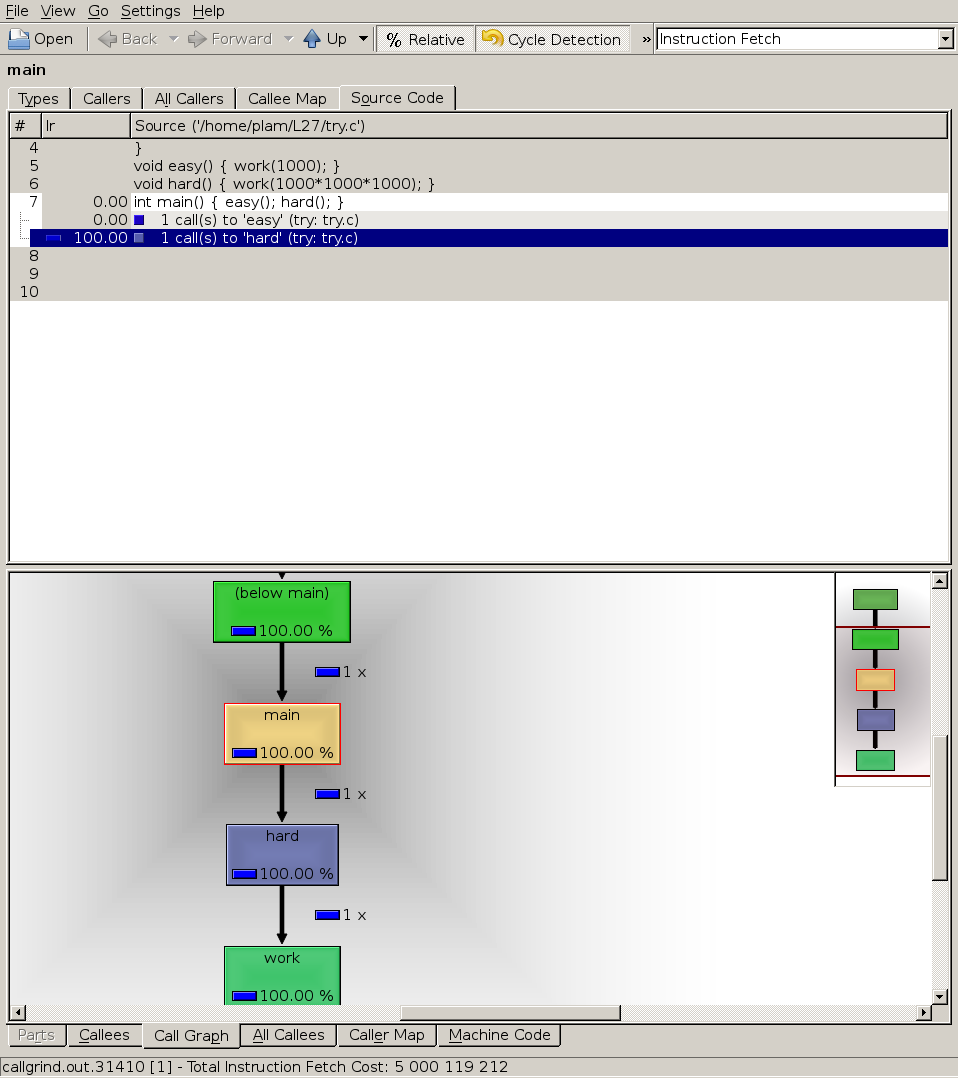
\includegraphics[width=.4\textwidth]{images/kcachegrind}
\end{center}

It properly reports that {\tt hard} takes all the time.
But we can still deceive it.

\paragraph{More Complex Example.} Let's look at this example.

\begin{minipage}{.4\textwidth}
\begin{lstlisting}[basicstyle=\scriptsize]
void worker1(int n) {
  volatile int i=0;
  while(i++<n);
}
void worker2(int n) {
  volatile int i=0;
  while(i++<n);
}
void manager(int n1, int n2) {
  worker1(n1);
  worker2(n2);
}
\end{lstlisting}
\end{minipage}
\begin{minipage}{.4\textwidth}
\begin{lstlisting}[basicstyle=\scriptsize]
void project1() {
  manager(1000, 1000000);
}
void project2() {
  manager(1000000, 1000);
}
int main() {
  project1();
  project2();
}
\end{lstlisting}
\end{minipage}

Now, {\tt worker2} takes all the time in {\tt project1},
and {\tt worker1} takes all the time in {\tt project2}.

Let's see how KCacheGrind does on this example.

\begin{center}
  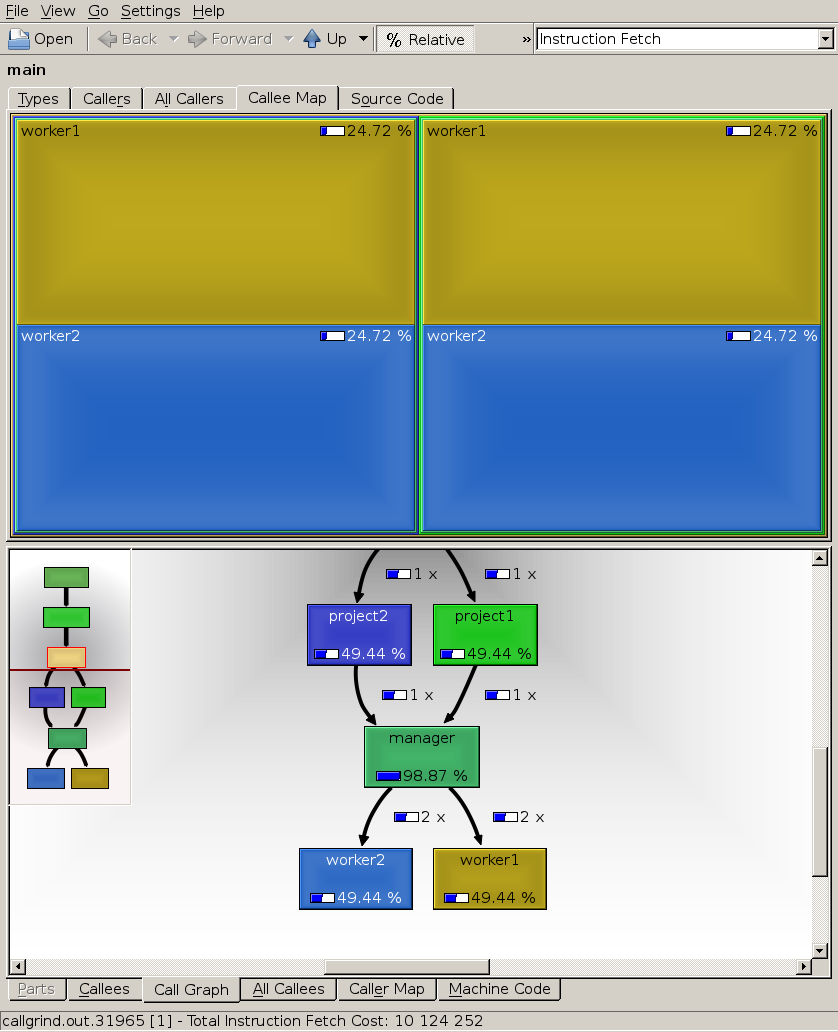
\includegraphics[width=.25\textwidth]{images/kcachegrind2}
\end{center}


The call graph, on the bottom, shows that 
{\tt worker1} and {\tt worker2} do each take about 50\% of time.
So do {\tt project2} and {\tt project1}. This is fine.
(I think gprof would correctly interpolate that too.)

However, KCacheGrind also lies, in the report on top. It is saying
that {\tt worker1} and {\tt worker2} doing half the work in each
project.  That's not what the code says. Why is it lying?

\begin{itemize}
\item gprof reports time spent in {\tt f()} and {\tt g()},
and how many times {\tt f()} calls {\tt g()}.
\item callgrind also reports 
time spent  in {\tt g()} when called from {\tt f()}, i.e. some calling-context information.
\item callgrind does \emph{not} report time spent in {\tt g()} when
     called from {\tt f()} when called from {\tt h()}.
     We don't get the {\tt project1} to {\tt manager} to {\tt worker1} link.
     (We have Edges but need Edge-Pairs).
\end{itemize}

\paragraph{Summary.} We've seen that some profiler results are exact;
some results are sampled; and some results are interpolated. If you understand the tool, you understand where it can go
wrong. 

Understand your tools!

\section*{Lies from Metrics}
While app-specific metrics can lie too, mostly we'll talk about CPU
perf counters today.

The reference here is a blog post by Paul Khuong~\cite{metrics}.

This goes back to {\tt mfence}, which we've seen before. It is used, for instance, in
spinlock implementations. Khuong found that his profiles said that spinlocking didn't take much time.
But empirically: eliminating spinlocks = better than expected! Hmm.

The next step is (as we do in this course) to create microbenchmarks to better understand what's
going on. The microbenchmark contained memory accesses to uncached locations, or computations,
surrounded by store pairs/mfence/locks. He used perf to evaluate the impact of mfence vs lock.

{\scriptsize
\begin{lstlisting}
# for locks:
$ perf annotate -s cache_misses
[...]
    0.06 :        4006b0:       and    %rdx,%r10
    0.00 :        4006b3:       add    $0x1,%r9
    ;; random (out of last level cache) read
    0.00 :        4006b7:       mov    (%rsi,%r10,8),%rbp
   30.37 :        4006bb:       mov    %rcx,%r10
    ;; foo is cached, to simulate our internal lock
    0.12 :        4006be:       mov    %r9,0x200fbb(%rip)
    0.00 :        4006c5:       shl    $0x17,%r10
    [... Skipping arithmetic with < 1% weight in the profile]
    ;; locked increment of an in-cache "lock" byte
    1.00 :        4006e7:       lock incb 0x200d92(%rip)
   21.57 :        4006ee:       add    $0x1,%rax
    [...]
    ;; random out of cache read
    0.00 :        400704:       xor    (%rsi,%r10,8),%rbp
   21.99 :        400708:       xor    %r9,%r8
    [...]
    ;; locked in-cache decrement
    0.00 :        400729:       lock decb 0x200d50(%rip)
   18.61 :        400730:       add    $0x1,%rax
    [...]
    0.92 :        400755:       jne    4006b0 <cache_misses+0x30>
\end{lstlisting}
}

We can see that in the lock situation, reads take 30 + 22 = 52\% of runtime,
while locks take 19 + 21 = 40\% of runtime.

{\scriptsize
\begin{lstlisting}
# for mfence:
$ perf annotate -s cache_misses
[...]
    0.00 :        4006b0:       and    %rdx,%r10
    0.00 :        4006b3:       add    $0x1,%r9
    ;; random read
    0.00 :        4006b7:       mov    (%rsi,%r10,8),%rbp
   42.04 :        4006bb:       mov    %rcx,%r10
    ;; store to cached memory (lock word)
    0.00 :        4006be:       mov    %r9,0x200fbb(%rip)
    [...]
    0.20 :        4006e7:       mfence 
    5.26 :        4006ea:       add    $0x1,%rax
    [...]
    ;; random read
    0.19 :        400700:       xor    (%rsi,%r10,8),%rbp
   43.13 :        400704:       xor    %r9,%r8
    [...]
    0.00 :        400725:       mfence 
    4.96 :        400728:       add    $0x1,%rax
    0.92 :        40072c:       add    $0x1,%rax
    [...]
    0.36 :        40074d:       jne    4006b0 <cache_misses+0x30>
\end{lstlisting}
}
Looks like the reads take 85\% of runtime,
while the mfence takes 15\% of runtime.

Metrics lie, though, and when you focus on the metrics as opposed to what you
actually care about, it's easy to be led astray.

In this case, what we actually care about is the total \# of cycles.

    \begin{tabular}{lr}
    No atomic/fence:& 2.81e9 cycles\\
    lock inc/dec: & 3.66e9 cycles\\
    mfence: & 19.60e9 cycles
    \end{tabular}

That 15\% number is a total lie.
Profilers, even using CPU expense counts, drastically underestimate the impact of mfence,
and overestimate the impact of locks.

This is because mfence causes a pipeline flush, and the resulting 
costs get attributed to instructions being flushed, not to the mfence itself.


\section*{The Long Tail}

Our source here is the blog post by Dan Luu~\cite{perf-tracing}. Suppose we have a task that's going to get distributed over multiple computers (like a search). If we look at the latency distribution, the problem is mostly that we see a long tail of events and when we are doing a computation or search where we need all the results, we can only go as the slowest step. Let's take a look at a histogram of disk read latencies, where we are performing a 64 kB read, also from that source:

\begin{center}
	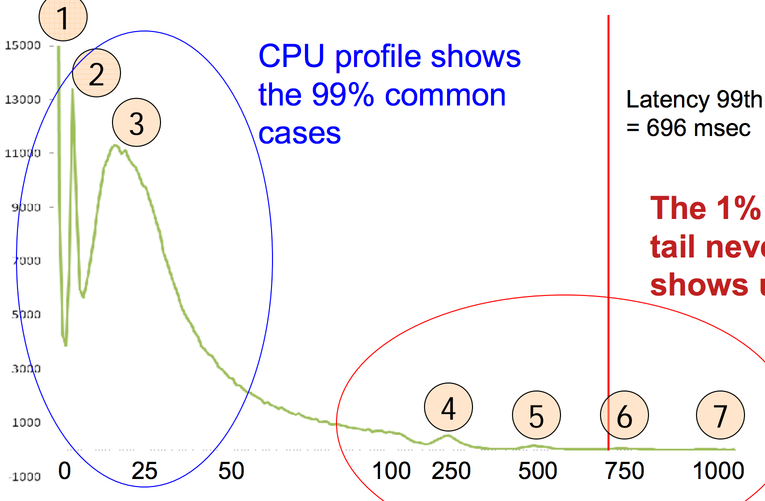
\includegraphics[width=0.65\textwidth]{images/disk_tail.png}
\end{center}

Let's break it down. Peak 1 corresponds to something cached in RAM---best case scenario. Peak 2 is at around 3ms, which is too fast for spinning and seeking magnetic hard disks, but it's fast enough for reading something from the disk cache via the PCI-Express interface. Peak 3 is obviously disk seek and read times, somewhere around 25ms. 

These numbers don't look terrible, except for the fact that we have peaks at 250, 500, 750, and 1000 ms and the 99th percentile is some 696ms which is a very, very long time. Sampling profilers are not very good at finding these things, because they throw everything into various buckets and therefore we get averages. The averages are misleading, though, because we have these weird outliers that take dramatically longer. Averages are nice as long as our data is also reasonably ``nice''.

So what actually happened? Well, from~\cite{perf-tracing}: The investigator found out that the cause was kernel throttling of the CPU for processes that went beyond their usage quota. To enforce the quota, the kernel puts all of the relevant threads to sleep until the next multiple of a quarter second. When the quarter-second hand of the clock rolls around, it wakes up all the threads, and if those threads are still using too much CPU, the threads get put back to sleep for another quarter second. The phase change out of this mode happens when, by happenstance, there aren't too many requests in a quarter second interval and the kernel stops throttling the threads. After finding the cause, an engineer found that this was happening on 25\% of disk servers at Google, for an average of half an hour a day, with periods of high latency as long as 23 hours. This had been happening for three years.

Further limitations of sampling profilers emerge, as demonstrated in this graph, also from~\cite{perf-tracing}, showing the data we get out of our sampling profiler if we take a look at Lucene (a search indexer):

\begin{center}
	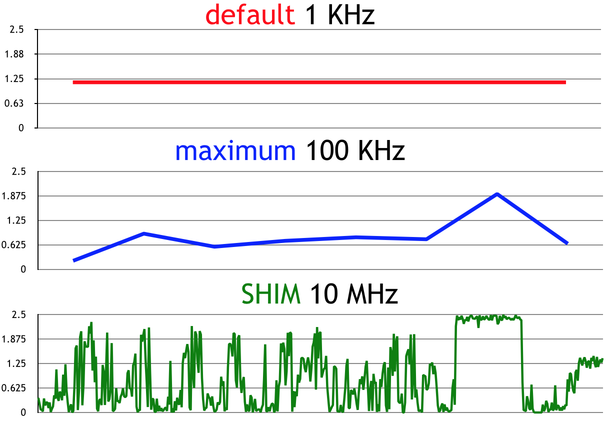
\includegraphics[width=0.5\textwidth]{images/perf-sample.png}
\end{center}

So at the default sampling interval for perf we see\ldots nothing interesting whatsoever. If we bump up to the max sampling frequency of perf, we get a moderately more interesting graph, but not much. If we use a different tool and can sample at a dramatically higher rate, then we end up with something way more useful. So we're left to wonder why does perf sample so infrequently, and how does SHIM get around this?

Well, for one thing, perf samples are done with interrupts. Processing interrupts takes a fair amount of time and if you crank up the rate of interrupts, before long, you are spending all your time handling the interrupts rather than doing useful work. SHIM gets around this by being more invasive---it adds some periodically executed code that puts information out whenever there is an appropriate event (e.g., function return). This produces a bunch of data which can be dealt with later to produce something useful.

  \paragraph{Algorithmic profiling.} Coppa et al~\cite{coppa2014input} have proposed another profiling tool,
  {\tt aprof}.
  \url{https://code.google.com/p/aprof/}
{
  \begin{quote}
  aprof is a Valgrind tool for performance profiling designed to help developers discover hidden asymptotic inefficiencies in the code. From one or more runs of a program, aprof measures how the performance of individual routines scales as a function of the input size, yielding clues to its growth rate and to the "big-O" of the program.
  \end{quote}
  }

\paragraph{Summary} We saw a bunch of lies today: calling-context lies and perf attribution
lies. To avoid being bitten by lies, remember to focus on the metric you actually care about,
and understand how your tools work.










\chapter*{27 --- Memory Profiling}

\addcontentsline{toc}{chapter}{27 --- Memory Profiling}

\section*{\st{Memory Profiling} Return to Asgard}

Thus far we have focused on CPU profiling. Other kinds of profiling got some mention, but they're not the only kind of profiling we can do. Memory profiling is also a thing, and specifically we're going to focus on heap profiling. We kind of touched on the subject a little bit earlier when we looked at finding memory leaks. The ideas are the same: we don't want to leak memory, but remember that last category (other than suppressed), ``Still Reachable'', things that remained allocated and we still had pointers to them, but were not properly deallocated? Right, we care about them too, and for that we want to do heap profiling.

If we don't look after those things, we're just using more and more memory over time. That likely means more paging and the potential for running out of heap space altogether. Again, the memory isn't really lost, because we could free it.

Well, let's start with where we left off. Returning to the realm of Asgard, we're going to call again on our old friend Valgrind. Except this time we're going to use a fourth tool in it: Massif. This is, obviously, a joke on ``massive'', combined with the name Sif, a Norse goddess associated with the earth (and in the Marvel movies, Shieldmaiden to Thor). While we're on the subject, Sif has an axe (shield?) to grind with Loki, because at some point he cut off her golden hair (and in the Marvel films, it grew back in dark). That Loki---what a trickster! Right, we're digressing\ldots what do you mean the course isn't ECE 459: Norse Mythology?!

So what does Massif do? It will tell you about how much heap memory your program is using, and also how the situation got to be that way. So let's start with the example program from the documentation~\cite{massif}:

{\scriptsize
\begin{verbatim}
#include <stdlib.h>

void g ( void ) {
    malloc( 4000 );
}

void f ( void ) {
    malloc( 2000 );
    g();
}

int main ( void ) {
    int i;
    int* a[10];

    for ( i = 0; i < 10; i++ ) {
        a[i] = malloc( 1000 );
    }
    f();
    g();

    for ( i = 0; i < 10; i++ ) {
        free( a[i] );
    }
    return 0;
}
\end{verbatim}
}

After we compile (remember the \texttt{-g} option for debug symbols), run the command:
{\scriptsize
\begin{verbatim}
jz@Loki:~/ece459$ valgrind --tool=massif ./massif
==25187== Massif, a heap profiler
==25187== Copyright (C) 2003-2013, and GNU GPL'd, by Nicholas Nethercote
==25187== Using Valgrind-3.10.1 and LibVEX; rerun with -h for copyright info
==25187== Command: ./massif
==25187== 
==25187== 
\end{verbatim}
}

Doesn't that look useful?! What happened? Your program executed slowly, as is always the case with any of the Valgrind toolset, but you don't get summary data on the console like we did with Valgrind or helgrind or cachegrind. Weird. What we got instead was the file \texttt{massif.out.25187} (matches the PID of whatever we ran). This file, which you can open up in your favourite text editor is not especially human readable, but it's not incomprehensible like the output from cachegrind (``Aha, a 1 in column 4 of line 2857. That's what's killing our performance!''). There is an associated tool for summarizing and interpreting this data in a much nicer way: \texttt{ms\_print}, which has nothing whatsoever to do with Microsoft. Promise.

If we look at the output there (hint: pipe the output to \texttt{less} or something, otherwise you get a huge amount of data thrown at the console), it looks much more user friendly.

{\scriptsize
\begin{verbatim}

    KB
19.71^                                                                       #
     |                                                                       #
     |                                                                       #
     |                                                                       #
     |                                                                       #
     |                                                                       #
     |                                                                       #
     |                                                                       #
     |                                                                       #
     |                                                                       #
     |                                                                       #
     |                                                                       #
     |                                                                       #
     |                                                                       #
     |                                                                       #
     |                                                                       #
     |                                                                      :#
     |                                                                      :#
     |                                                                      :#
     |                                                                      :#
   0 +----------------------------------------------------------------------->ki
     0                                                                   111.9
\end{verbatim}
}

Now wait a minute. This bar graph might be user friendly but it's not exactly what I'd call... useful, is it? For a long time, nothing happens, then... kaboom! According to the docs, what actually happened here is, we gave in a trivial program where most of the CPU time was spent doing the setup and loading and everything, and the trivial program ran for only a short period of time, right at the end. So for a relatively short program we should tell Massif to care more about the bytes than the CPU cycles, with the \verb+--time-unit=B+ option. Let's try that.

{\scriptsize
\begin{verbatim}

    KB
19.71^                                               ###                      
     |                                               #                        
     |                                               #  ::                    
     |                                               #  : :::                 
     |                                      :::::::::#  : :  ::               
     |                                      :        #  : :  : ::             
     |                                      :        #  : :  : : :::          
     |                                      :        #  : :  : : :  ::        
     |                            :::::::::::        #  : :  : : :  : :::     
     |                            :         :        #  : :  : : :  : :  ::   
     |                        :::::         :        #  : :  : : :  : :  : :: 
     |                     @@@:   :         :        #  : :  : : :  : :  : : @
     |                   ::@  :   :         :        #  : :  : : :  : :  : : @
     |                :::: @  :   :         :        #  : :  : : :  : :  : : @
     |              :::  : @  :   :         :        #  : :  : : :  : :  : : @
     |            ::: :  : @  :   :         :        #  : :  : : :  : :  : : @
     |         :::: : :  : @  :   :         :        #  : :  : : :  : :  : : @
     |       :::  : : :  : @  :   :         :        #  : :  : : :  : :  : : @
     |    :::: :  : : :  : @  :   :         :        #  : :  : : :  : :  : : @
     |  :::  : :  : : :  : @  :   :         :        #  : :  : : :  : :  : : @
   0 +----------------------------------------------------------------------->KB
     0                                                                   29.63

\end{verbatim}
}

Neat. Now we're getting somewhere. We can see that 25 snapshots were taken. It will take snapshots whenever there are appropriate allocation and deallocation statements, up to a configurable maximum, and for a long running program, toss some old data if necessary. Let's look in the documentation to see what the symbols mean (they're not just to look pretty). So, from the docs~\cite{massif}:

\begin{itemize}
\item Most snapshots are normal (they have just basic information) They use the `:' characters.

\item Detailed snapshots are shown with `@' characters.  By default, every 10th snapshot is detailed.

\item There is at most one peak snapshot. The peak snapshot is a detailed snapshot, and records the point where memory consumption was greatest. The peak snapshot is represented in the graph by a bar consisting of `\#' characters.
\end{itemize}

As a caveat, the peak can be a bit inaccurate. Peaks are only recorded when a deallocation happens. This just avoids wasting time recording a peak and then overwriting it; if you are allocating a bunch of blocks in succession (e.g., in assignment 1, a bunch of structs that have a buffer) then you would constantly be overwriting the peak over and over again. Also, there's some loss of accuracy to speed things up. Well, okay.

So let's look at the snapshots. We'll start with the normal ones. There are 9 of those, numbers 0 through 8:

{\scriptsize
\begin{verbatim}
--------------------------------------------------------------------------------
  n        time(B)         total(B)   useful-heap(B) extra-heap(B)    stacks(B)
--------------------------------------------------------------------------------
  0              0                0                0             0            0
  1          1,016            1,016            1,000            16            0
  2          2,032            2,032            2,000            32            0
  3          3,048            3,048            3,000            48            0
  4          4,064            4,064            4,000            64            0
  5          5,080            5,080            5,000            80            0
  6          6,096            6,096            6,000            96            0
  7          7,112            7,112            7,000           112            0
  8          8,128            8,128            8,000           128            0
\end{verbatim}
}

The columns are pretty much self explanatory, with a couple exceptions. The time(B) column corresponds to time measured in allocations thanks to our choice of the time unit at the command line. The extra-heap(B) represents internal fragmentation\footnote{Remember from operating systems: if the user asked for some $n$ bytes where $n$ is not a nice multiple the returned block may be ``rounded up''. So a request for 1000 bytes is bumped up to 1016 bytes in this example. The extra space is ``wasted'' but it's nicer than having a whole bunch of little tiny useless fragments of the heap to be managed.} in the blocks we received. The stacks column shows as zero because by default, Massif doesn't look at the stack. It's a heap profiler, remember?

Number 9 is a ``detailed'' snapshot, so I've separated it out, and reproduced the headers there to make this a little easier to remember what they are.

{
\begin{verbatim}
--------------------------------------------------------------------------------
  n        time(B)         total(B)   useful-heap(B) extra-heap(B)    stacks(B)
--------------------------------------------------------------------------------
  9          9,144            9,144            9,000           144            0
98.43% (9,000B) (heap allocation functions) malloc/new/new[], --alloc-fns, etc.
->98.43% (9,000B) 0x4005BB: main (massif.c:17)
\end{verbatim}
}

So the additional information we got here is a reflection of where our heap allocations took place. Thus far, all the allocations took place on line 17 of the program, which was \texttt{  a[i] = malloc( 1000 ); } inside that for loop.

Then let's look at the peak snapshot (again, trimmed a bit to call out exactly what we need to see here):

{
\begin{verbatim}
--------------------------------------------------------------------------------
  n        time(B)         total(B)   useful-heap(B) extra-heap(B)    stacks(B)
--------------------------------------------------------------------------------
 14         20,184           20,184           20,000           184            0
99.09% (20,000B) (heap allocation functions) malloc/new/new[], --alloc-fns, etc.
->49.54% (10,000B) 0x4005BB: main (massif.c:17)
| 
->39.64% (8,000B) 0x400589: g (massif.c:4)
| ->19.82% (4,000B) 0x40059E: f (massif.c:9)
| | ->19.82% (4,000B) 0x4005D7: main (massif.c:20)
| |   
| ->19.82% (4,000B) 0x4005DC: main (massif.c:22)
|   
->09.91% (2,000B) 0x400599: f (massif.c:8)
  ->09.91% (2,000B) 0x4005D7: main (massif.c:20)

\end{verbatim}
}

Massif has found all the allocations in this program and distilled them down to a tree structure that traces the path through which all of these various memory allocations occurred. So not just where the \texttt{malloc} call happened, but also how we got there.

When program termination occurs we get a final output of what blocks remains allocated and where they come from. These point to memory leaks, incidentally, and valgrind would not be amused with us.

{
\begin{verbatim}
 24         30,344           10,024           10,000            24            0
99.76% (10,000B) (heap allocation functions) malloc/new/new[], --alloc-fns, etc.
->79.81% (8,000B) 0x400589: g (massif.c:4)
| ->39.90% (4,000B) 0x40059E: f (massif.c:9)
| | ->39.90% (4,000B) 0x4005D7: main (massif.c:20)
| |   
| ->39.90% (4,000B) 0x4005DC: main (massif.c:22)
|   
->19.95% (2,000B) 0x400599: f (massif.c:8)
| ->19.95% (2,000B) 0x4005D7: main (massif.c:20)
|   
->00.00% (0B) in 1+ places, all below ms_print's threshold (01.00%)
\end{verbatim}
}

In fact, if I ask valgrind what it thinks of this program, it says:

{\scriptsize
\begin{verbatim}
jz@Loki:~/ece459$ valgrind ./massif
==25775== Memcheck, a memory error detector
==25775== Copyright (C) 2002-2013, and GNU GPL'd, by Julian Seward et al.
==25775== Using Valgrind-3.10.1 and LibVEX; rerun with -h for copyright info
==25775== Command: ./massif
==25775== 
==25775== 
==25775== HEAP SUMMARY:
==25775==     in use at exit: 10,000 bytes in 3 blocks
==25775==   total heap usage: 13 allocs, 10 frees, 20,000 bytes allocated
==25775== 
==25775== LEAK SUMMARY:
==25775==    definitely lost: 10,000 bytes in 3 blocks
==25775==    indirectly lost: 0 bytes in 0 blocks
==25775==      possibly lost: 0 bytes in 0 blocks
==25775==    still reachable: 0 bytes in 0 blocks
==25775==         suppressed: 0 bytes in 0 blocks
==25775== Rerun with --leak-check=full to see details of leaked memory
==25775== 
==25775== For counts of detected and suppressed errors, rerun with: -v
==25775== ERROR SUMMARY: 0 errors from 0 contexts (suppressed: 0 from 0)
\end{verbatim}
}

So probably a good idea to run valgrind first and make it happy before we go into figuring out where heap blocks are going with Massif. Okay, what to do with the information from Massif, anyway? It should be pretty easy to act upon this information. Start with the peak snapshot (worst case scenario) and see where that takes you (if anywhere). You can probably identify some cases where memory is hanging around unnecessarily. 

\newpage
Things to watch out for:
\begin{itemize}
\item memory usage climbing over a long period of time, perhaps slowly, but never really decreasing---memory is filling up somehow with some junk? 
\item large spikes in the graph---why so much allocation and deallocation in a short period?
\end{itemize}

Other cool things we can do with Massif~\cite{massif}:

\begin{itemize}
	\item Look into stack allocation (\verb+--stacks=yes+) option. This slows stuff down a lot, and not really necessary since we want to look at heap.
	\item Look at the children of a process (anything split off with \texttt{fork}) if desired.
	\item Check low level stuff: if we're doing something other than \texttt{malloc}, \texttt{calloc}, \texttt{new}, etc. and doing low level stuff like \texttt{mmap} or \texttt{brk} that is usually missed, but we can do profiling at page level (\verb+--pages-as-heap=yes+).
\end{itemize}

As is often the case, we have examined how the tool works on a trivial program. As a live demo, let's see what happens when we take the program complexity up a little bit by (1) looking at the search program we saw in the earlier talk about valgrind; and (2) looking at the original (unmodified) paster.c file from assignment 1 (and then perhaps fixing it and going on). Depending on time available, we may look at some more complex programs.










\chapter*{28 --- Profiler Guided Optimization (POGO)}

\addcontentsline{toc}{chapter}{28 --- Profiler Guided Optimization (POGO)}

\section*{Profiler Guided Optimization (POGO)}

In 2015 we were fortunate enough to have a guest lecture from someone at Microsoft actually in the room to give the guest lecture on the subject of Profile Guided Optimization (or POGO). Try as I might, I was not able to convince him to fly in just for this lecture. For an alternative take on the subject, you could watch the full video at \url{https://www.youtube.com/watch?v=zEsdBcu4R00}. We'll use an excerpt in this lecture.

The compiler does a great deal of static analysis of the code you've written and makes its best guesses about what is likely to happen. The canonical example for this is branch prediction: there is an if-else block and the compiler will then guess about which is more likely and optimize for that version. Consider three examples from~\cite{pogo}:

\begin{center}
	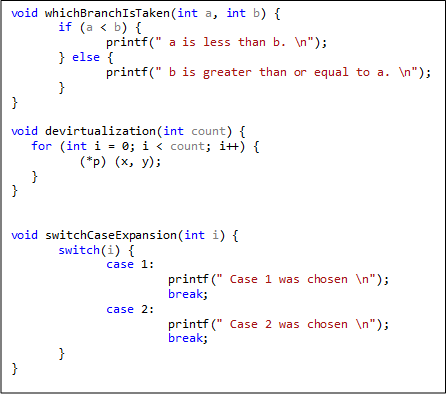
\includegraphics[width=0.5\textwidth]{images/4621codesnippet.png}
\end{center}

Just looking at this, which is more likely, \texttt{a < b} or \texttt{a >= b}? Assuming there's no other information in the system the compiler can believe that one is more likely than the other, or having no real information, use a fallback rule. This works, but what if we are wrong? Suppose the compiler decides it is likely that \texttt{a} is the larger value and it optimizes for that version. However, it is only the case 5\% of the time, so most of the time the prediction is wrong. That's unpleasant. But the only way to know is to actually run the program.

There are similar questions raised for the other two examples. What is the ``normal'' value for some pointer \texttt{p}? If we do not know, the compiler cannot do devirtualization (replace this virtual call with a real one). Same thing with \texttt{i}: what is its typical value? If we know that, it is our prediction. Actually, in a switch-case block with many options, could we rank them in descending order of likelihood?

There exists a solution to this, and it is that we can give hints to the compiler, but that's a manual process. Automation is a good thing and this lecture is about that. These sorts of things already exist for Java! The Java HotSpot virtual machine will update its predictions on the fly. There are some initial predictions and if they turn out to be wrong, the Just In Time compiler will replace it with the other version. That's neat! I don't know for certain but I suspect the .NET runtime will do the same for something like C\#. But this is C(++) (Sparta) and we don't have that: the compiler runs and it does its job and that's it; the program is never updated with newer predictions if more data becomes known.

Solving this problem is the goal of POGO. It is taking the data from some actual runs of the program and using that to inform the predictions. This necessitates a multi-step compile: first compile the code, run it to collect data, then recompile the code using the data we collected. Let's expand on all three steps.

Step one is to generate an executable with instrumentation. The compiler inserts a bunch of probes into the generated code that are used to record data. Three types of probe are inserted: function entry probes, edge probes, and value probes.  A function entry probe, obviously, counts how many times a particular function is called. An edge probe is used to count the transitions (which tells us whether an if branch is taken or the else condition). Value probes are interesting; they are used to collect a histogram of values. Thus, we can have a small table that tells us the frequency of what is given in to a \texttt{switch} statement. When this phase is complete, there is an instrumented executable and an empty database file where the training data goes~\cite{pogo}.

Step two is training day: run the instrumented executable through real-world scenarios. Ideally you will spend the training time on the performance-critical sections. It does not have to be a single training run, of course, data can be collected from as many runs as desired.   Still, it is important to note that you are not trying to exercise every part of the program (this is not unit testing); instead it should be as close to real-world-usage as can be accomplished. In fact, trying to use every bell and whistle of the program is counterproductive; if the usage data does not match real world scenarios then  the compiler has been given the wrong information about what is important. Or you might end up teaching it that almost nothing is important...

Step three is a recompile. This time, in addition to the source files, the training data is fed into the compiler for a second compile, and this data is applied to produce a better output executable than could be achieved by static analysis alone.

The Intel Developer Zone explains the process in a handy infographic\footnote{Source: \url{https://software.intel.com/en-us/node/522721}} :

\begin{center}
	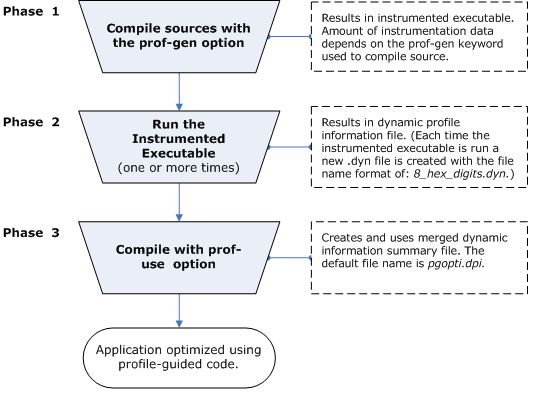
\includegraphics[width=0.5\textwidth]{images/pogo-workflow.jpg}
\end{center}

It is not necessary to do all three steps for every build. Old training data can be re-used until the code base has diverged significantly enough from the instrumented version. According to~\cite{pogo}, the recommended workflow is for one developer to perform these steps and check the training data into source control so that other developers can make use of it in their builds.

What does it mean for it to be better? We have already looked at an example about how to predict branches. Predicting it correctly will be faster than predicting it incorrectly, but this is not the only thing.  The algorithms will aim for speed in the areas that are ``hot'' (performance critical and/or common scenarios). The algorithms will alternatively aim to minimize the size of code of areas that are ``cold'' (not heavily used). It is recommended in~\cite{pogo} that less than 5\% of methods should be compiled for speed.

It is possible that we can combine multiple training runs and we can manually give some suggestions of what scenarios are important. Obviously the more a scenario runs in the training data, the more important it will be, as far as the POGO optimization routine is concerned, but multiple runs can be merged with user assigned weightings.

With the theory behind us, perhaps a demonstration about how it works is in order. Let us consider an example using the N-Body problem. Let's look at the video \url{https://www.youtube.com/watch?v=zEsdBcu4R00&t=21m45s} (from 21:45 to 34:23).


\subsection*{Behind the Scenes}

In the optimize phase, the training data is used to do the following optimizations~\cite{pogo2}:

\begin{multicols}{2}
\begin{enumerate}
\item Full and partial inlining
\item Function layout
\item Speed and size decision
\item Basic block layout 
\item Code separation
\item Virtual call speculation
\item Switch expansion
\item Data separation
\item Loop unrolling
\end{enumerate}
\end{multicols}

For the most part we should be familiar with the techniques that are listed as being other compiler optimizations we have previously discussed. The new ones are (3) speed and size decision, which we have just covered; and items (4) and (5) which relate to how to pack the generated code in the binary.

According to~\cite{pogo2} the majority of the performance gains relate to the inlining decisions. These decisions are based on the call graph path profiling: the behaviour of function \texttt{foo} may be very different when calling it from \texttt{bar} than it is when calling it from function \texttt{baz}\footnote{Why are these the example function names?! It's kind of like Alice and Bob...}. Great, let's look at this call graph from~\cite{pogo2}:

\begin{center}
	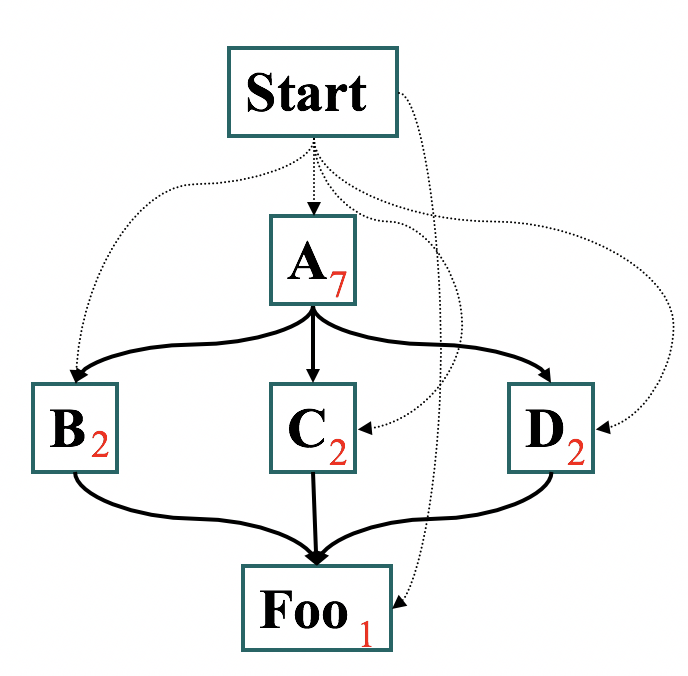
\includegraphics[width=0.25\textwidth]{images/callpaths.png}
\end{center}

Quick analysis of this code would have us find all the ways in which the functions might call each other. In total, there are 14 paths in this code, seven of which get us to function \texttt{Foo}.  

Consider another diagram showing the relationships between functions, in which the numbers on the edges represent the number of invocations~\cite{pogo2}:

\begin{center}
	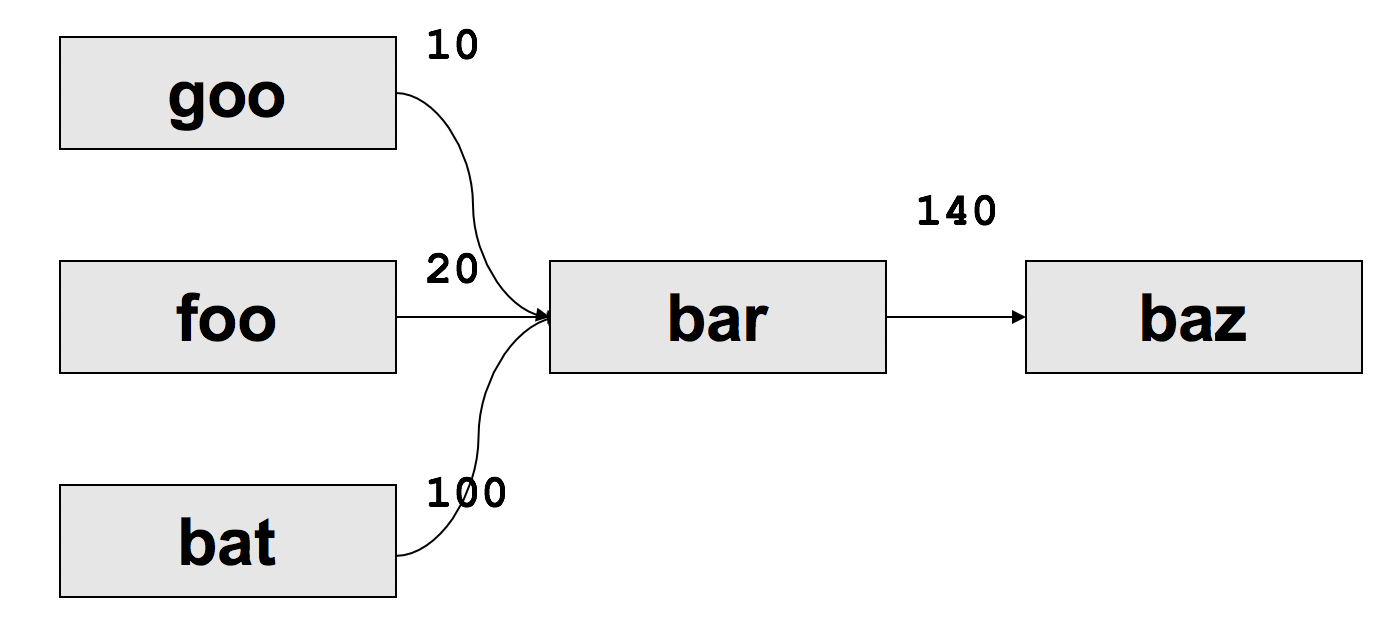
\includegraphics[width=0.4\textwidth]{images/callpaths2.png}
\end{center}

When considering what to do here, POGO takes the view like this~\cite{pogo2}:

\begin{center}
	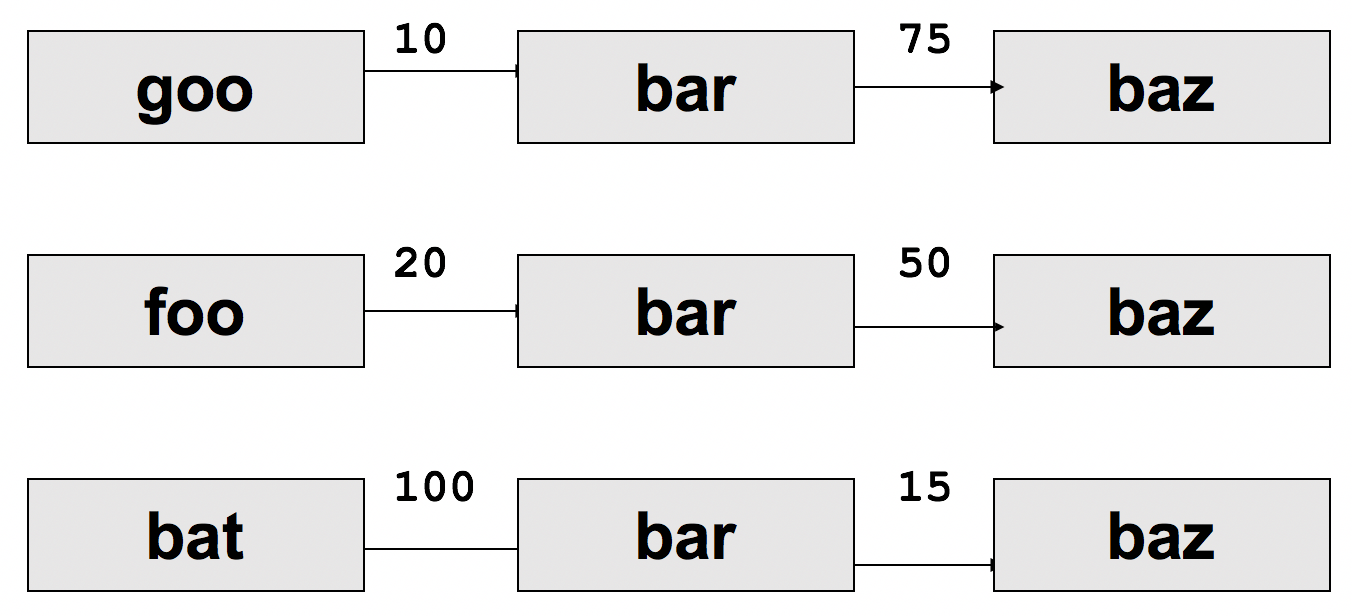
\includegraphics[width=0.4\textwidth]{images/callpaths3.png}
\end{center}

Each part of the call path is considered separately, remembering that we want to inline where it makes sense for speed, but otherwise leave it alone because of code size increases. Inlining \texttt{bar} into \texttt{bat} makes sense, but not inlining \texttt{bar} into \texttt{goo} (because that increases the code size without significant performance benefits). It also makes sense for \texttt{baz} to get inlined into \texttt{bar}. This is illustrated below~\cite{pogo2}:

\begin{center}
	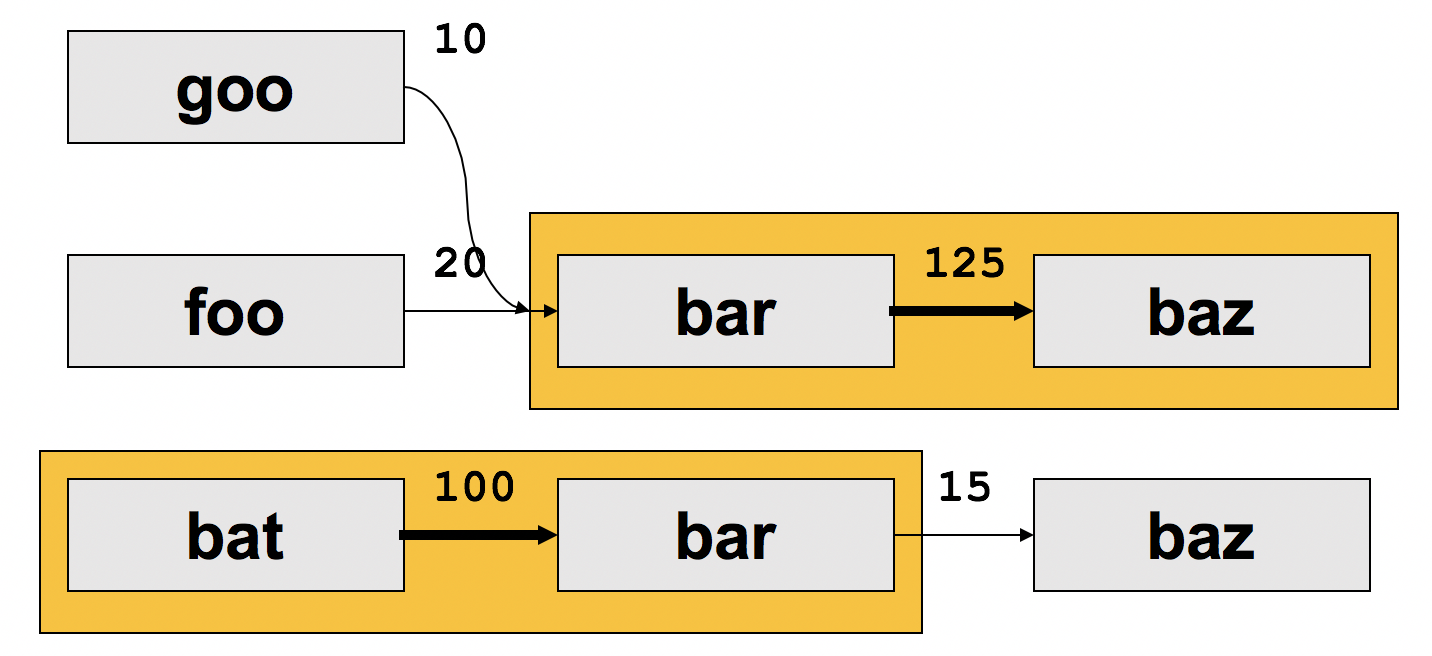
\includegraphics[width=0.4\textwidth]{images/callpaths4.png}
\end{center}

Packing the blocks is also done based on this call graph profiling. The most common cases will be put next to each other, and, where possible, subsequent steps are put next to each other. The more we can pack related code together, the fewer page faults we get by jumping to some other section, causing a cache miss... If the function being called is in the same page as the call, it has achieved ``page locality'' (and that is the goal!). This is represented visually~\cite{pogo2}:

\begin{center}
	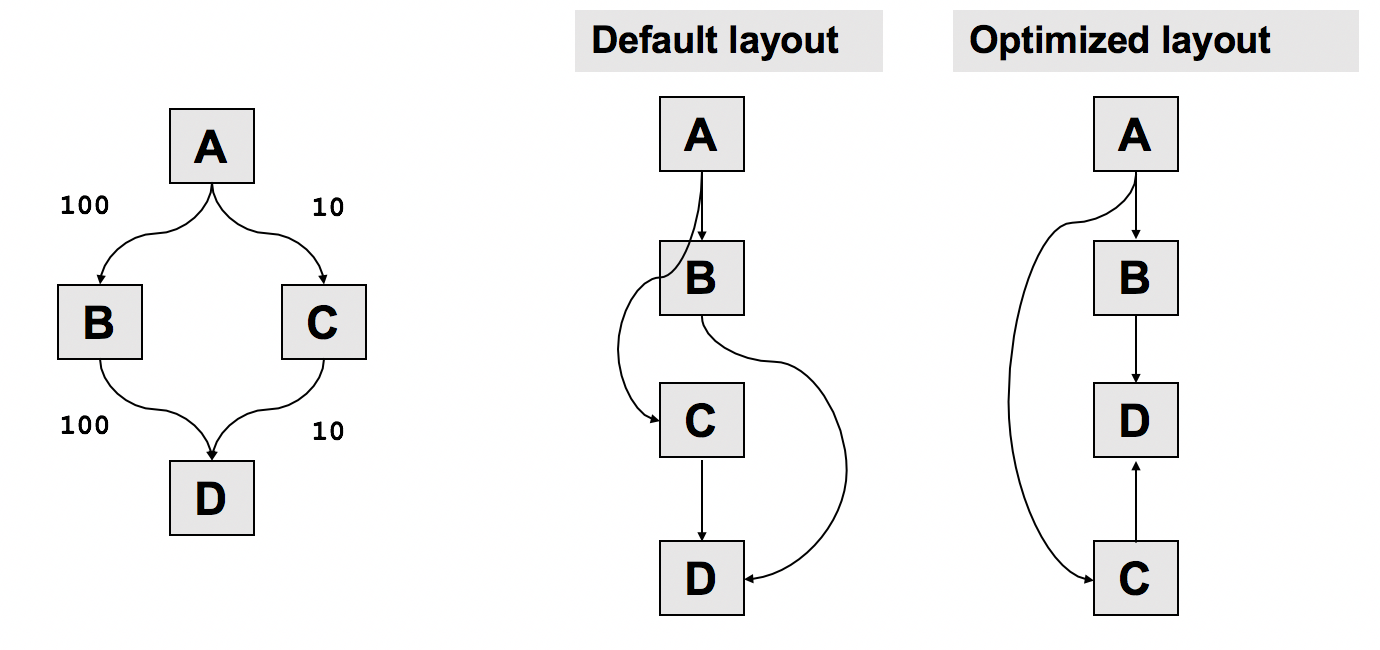
\includegraphics[width=0.6\textwidth]{images/blocklayout.png}
\end{center}

According to the author, the ``dead'' code goes in its own special block. I don't think they actually mean truly dead code, the kind that is compile-time determined to be unreachable, but instead they mean code that never gets invoked in any of the training runs.

So, to sum up, the training data is used to identify what branches are likely to be taken, inlines code where that is a performance increase, and tries to pack the binary code in such a way as to reduce cache misses/page faults. How well does it work?

\subsection*{Benchmark Results}

This table, condensed from~\cite{pogo2} summarizes the gains to be made. The application under test is a standard benchmark suite (Spec2K):

\begin{center}
\begin{tabular}{l|l|l|l|l|l}
	\textbf{Spec2k:} & \textbf{sjeng} & \textbf{gobmk} & \textbf{perl} & \textbf{povray} & \textbf{gcc}\\ \hline
	\textbf{App Size:} &  {Small} & {Medium} & {Medium} & {Medium} & {Large} \\ \hline
	\textbf{Inlined Edge Count} & 50\% & 53\% & 25\% & 79\% & 65\% \\ \hline
	\textbf{Page Locality} & 97\% & 75\% & 85\% & 98\% & 80\% \\ \hline
	\textbf{Speed Gain} & 8.5\% & 6.6\% & 14.9\% & 36.9\% & 7.9\% \\ 
\end{tabular}
\end{center}

There are more details in the source as to how many functions are used in a typical run and how many things were inlined and so on. But we get enough of an idea from the last row of how much we are speeding up the program, plus some information about why. We can speculate about how well the results in a synthetic benchmark translate to real-world application performance, but at least from this view it does seem to be a net gain.








\chapter*{29 --- Clusters \& Cloud Computing}

\addcontentsline{toc}{chapter}{29 --- Clusters \& Cloud Computing}

\section*{Clusters and cloud computing}
Everything we've seen so far has improved performance on a single
computer. Sometimes, you need more performance than you can get on a
single computer. If you're lucky, then the problem can be divided
among multiple computers. We'll survey techniques for programming for
performance using multiple computers; although there's overlap with
distributed systems, we're looking more at calculations here.

\subsection*{Message Passing} For the majority of this course, 
we've talked about shared-memory systems. Last week's discussion of
GPU programming moved away from that a bit: we had to explicitly
manage copying of data. Message-passing is yet another paradigm.  In
this paradigm, often we run the same code on a number of nodes. These
nodes may potentially run on different computers (a cluster),
which communicate over a network.

MPI, the \emph{Message Passing Interface}, is a de facto standard for
programming message-passing systems. Communication is explicit in MPI:
processes pass data to each other using {\tt MPI\_Send} and {\tt
  MPI\_Recv} calls. 

Relevant piece about the relevance of MPI today:~\cite{hpcmpi}

\paragraph{Hello, World in MPI.} As with OpenCL kernels,
the first thing to do when writing an MPI program is to
figure out what the current process is supposed to compute.
Here's fairly standard skeleton code for that,
from \url{http://www.dartmouth.edu/~rc/classes/intro_mpi/}:

{\small
\begin{lstlisting}[language=C]
#include <stdio.h>
#include <mpi.h>

int main (int argc, char * argv[])
{
  int rank, size;

  MPI_Init (&argc, &argv);	/* starts MPI */
  MPI_Comm_rank (MPI_COMM_WORLD, &rank);	/* get current process id */
  MPI_Comm_size (MPI_COMM_WORLD, &size);	/* get number of processes */
  printf( "Hello world from process %d of %d\n", rank, size );
  MPI_Finalize();
  return 0;
}
\end{lstlisting}
}

\paragraph{Simple communication example.} The slides and live coding example contain
a second MPI example which demonstrates {\tt MPI\_Send} and  {\tt MPI\_Recv} usage,
also found at \url{http://en.wikipedia.org/wiki/Message_Passing_Interface}.

\paragraph{Matrix multiplication example.} We'll next discuss the code 
from another MPI example. You can find the code at
\url{http://www.nccs.gov/wp-content/training/mpi-examples/C/matmul.c}.
I'll discuss the structure of the code and
include relevant excerpts. Here are the steps that the program uses
to compute the matrix product $AB$:

\begin{enumerate}
\item Initialize MPI, as in the Hello, World example.
\item If the current process is the master task (task id 0):
\begin{enumerate}
\item Initialize the matrices.
\item Send work to each worker task: row number (offset); number of rows;
row contents from $A$; complete contents of matrix $B$. For example,

{\scriptsize
\begin{verbatim}
MPI_Send(&a[offset][0], rows*NCA, MPI_DOUBLE, dest, mtype, MPI_COMM_WORLD);
\end{verbatim}
}

\item Wait for results from all worker tasks (\verb+MPI_Recv+).
\item Print results.
\end{enumerate}
\item For all other tasks:
\begin{enumerate}
\item Receive offset, number of rows, partial matrix $A$, and complete matrix $B$, using {\tt MPI\_Recv}, e.g.

{\scriptsize
\begin{verbatim}
MPI_Recv(&offset, 1, MPI_INT, MASTER, mtype, MPI_COMM_WORLD, &status);
\end{verbatim}
}
\item Do the computation.
\item Send the results back to the sender.
\end{enumerate}
\end{enumerate}

\paragraph{On communication complexity.} To write fast MPI programs,
keeping communication complexity down is key. Each step from multicore
machines to GPU programming to MPI brings with it an
order-of-magnitude decrease in communication bandwidth and a similar
increase in latency.

\subsection*{Cloud Computing}
Historically, if you wanted a cluster, you had to find a bunch of
money to buy and maintain a pile of expensive machines. Not anymore.
Cloud computing is perhaps way overhyped, but we can talk about 
one particular aspect of it, as exemplified by Amazon's Elastic
Compute Cloud (EC2).

Consider the following evolution:
\begin{itemize}
\item Once upon a time, if you wanted a dedicated server on the
  Internet, you had to get a physical machine hosted, usually in a
  rack somewhere. Or you could live with inferior shared hosting.
\item Virtualization meant that you could instead pay for part of a
  machine on that rack, e.g. as provided by {\tt slicehost.com}.  This
  is a win because you're usually not maxing out a computer, and you'd
  be perfectly happy to share it with others, as long as there are
  good security guarantees. All of the users can get root access.
\item Clouds enable you to add more machines on-demand. Instead of
  having just one virtual server, you can spin up dozens (or
  thousands) of server images when you need more compute
  capacity. These servers typically share persistent storage, also in
  the cloud. 
\end{itemize}

In cloud computing, you pay according to the number of machines, or
instances, that you've started up. Providers offer different instance
sizes, where the sizes vary according to the number of cores, local
storage, and memory. Some instances even have GPUs, but it seemed 
uneconomic to use this for Assignment 3. Instead we have the {\tt ecetesla} machines.

\paragraph{Launching Instances.} When you need more compute power,
you launch an instance. The input is a virtual machine image.  You use
a command-line or web-based tool to launch the instance.  After you've
launched the instance, it gets an IP address and is
network-accessible. You have full root access to that instance.

Amazon provides public images which run a variety of operating
systems, including different Linux distributions, Windows Server, and
OpenSolaris. You can build an image which contains the software you
want, including Hadoop and OpenMPI.

\paragraph{Terminating Instances.} A key part of cloud computing is
that, once you no longer need an instance, you can just shut it down
and stop paying for it. All of the data on that instance goes away.

\paragraph{Storing Data.} You probably want to keep some persistent results
from your instances. Basically, you can either mount a storage device,
also on the cloud (e.g. Amazon Elastic Block Storage); or, you can
connect to a database on a persistent server (e.g. Amazon SimpleDB or
Relational Database Service); or, you can store files on the Web
(e.g. Amazon S3). 

\section*{Movie Hour}
Let's take a humorous look at cloud computing: James Mickens' session from Monitorama PDX 2014. 

\begin{center}
\url{https://vimeo.com/95066828}
\end{center}









\chapter*{30 --- Profiling and Scalability}

\addcontentsline{toc}{chapter}{30 --- Profiling and Scalability}

\section*{Profiling and Scalability}

Following the discussion of profiling and our look into cloud computing, we should take some time to understand performance and scalability. Recall that what we want in scalability is that we can take our software from 1 user to 100 to 10 million. Finishing work faster helps, but it's not the only way. So to scale up, we probably need to do some profiling to find out what's slow, but we have some things we need to worry about when we want to get away from just working on our dev machines and into big numbers of users.

So we should respect the following principles, as outlined in~\cite{swps}.

\paragraph{Hardware Principle.} 
Scalability testing is very different from  QA testing (as if you actually test your code!) in that you will do development and QA on your local computer and all you really care about is whether the program produces the correct output ``fast enough''. That's fine, but it's no way to test if it scales. If you actually want to test for scalability and real world performance, you should be doing it on the machines that are going to run the program in the live environment. Why? Well, low-end systems have very different limiting factors. You might be limited by the 4GB of RAM in your laptop and that would go away in the 64GB of RAM server you're using. So you might spend a great deal of time worrying about RAM usage when it turns out it doesn't matter.

\paragraph{Reality Principle.}
It would be a good idea to use a ``real'' workload, as much as one can possibly simulate. Legal reasons might prevent you from using actual customer data, but you should be trying to use the best approximation of it that you have. If you only generate some test data, you may not accurately represent the way the users are going to behave the system. Your test set run summary reports occasionally... your users might run them every hour. 

\paragraph{Volume Principle.}
``More is the new more.'' It's okay to use lighter workloads for regression testing and things like that, but if you actually want to see how your system performs under pressure, you actually need to put it under pressure. You can simulate pressure by limiting RAM or running something very CPU-intensive concurrently, but it's just not the same.

These tests, incidentally, are of great interest to the customers, who would like to know that you can deliver. 

\paragraph{Reproducibility and Regression Testing.}
Your results will need to be reproducible. Remember that good programming practice says that unit tests should be run, and re-run to make sure it all works. The same is true in your performance tests. Just as we don't want to see old bugs cropping up again, old (solved) performance issues are not nice to see either. Or a new change that slows the whole program down is not a success either. So please, have regression testing and performance regression testing.

\section*{Characterizing Performance \& Scalability Problems}

Now that we have some principles, let's get to the application of these principles. It is desirable to characterize problems, in quantitative terms, so that we can solve it. We will use an example from~\cite{swps}. The application is deployed on two systems -- one application server and one database server. The data is stored on an external SAN with RAID0 configuration. A Java\footnote{Quit snickering... Java isn't THAT slow... anymore...} program ran to simulate object creation with 15 threads. The performance metric is objects created per second. Let's take a look at the results, also from~\cite{swps}:

\begin{center}
	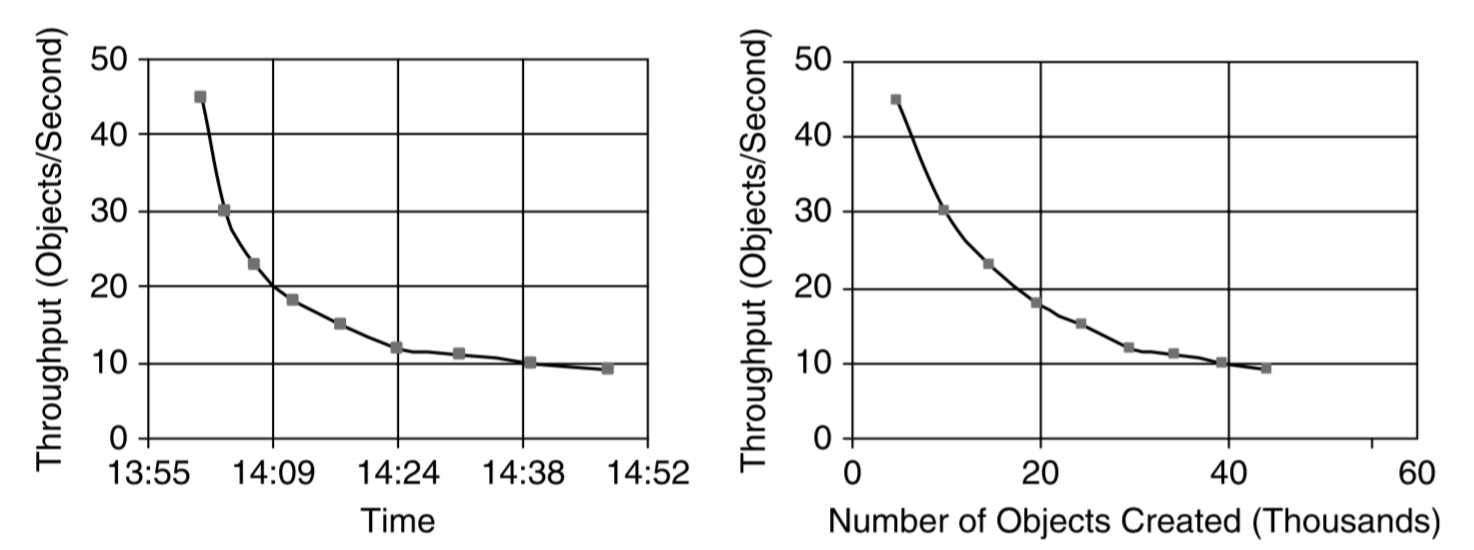
\includegraphics[width=0.85\textwidth]{images/batch-job-scalability.png}
\end{center}

This is, to use the technical term, ``not good''. The throughput deteriorates rapidly from about 45 objects per second down to 9 objects per second, with about 45~000 objects created at the end of the test. This is not the trend we want so see. What if we need to create 500~000 objects? 5~000~000? We have a problem. So we had best find out what's going wrong... and why.

\begin{quote}
\textit{It is a capital mistake to theorize before one has data. Insensibly one begins to twist facts to suit theories, instead of theories to suit facts.}
\end{quote}
\hfill - Sherlock Holmes (\textit{A Scandal in Bohemia}; Sir Arthur Conan Doyle)

Keeping the wisdom of Mr. Holmes in mind, we need to collect evidence before reaching conclusions. At a high level we probably have four potential culprits to start with:
\begin{enumerate}
	\item CPU
	\item Memory
	\item Disk
	\item Network
\end{enumerate}

These are, obviously, more categories than specific causes, but they are starting points for further investigation. They are listed in some numerical order, but there is no reason why one would have to investigate them in the order defined there.

CPU is probably the easiest of these to diagnose. Something like \texttt{top} or Task Manager will tell you pretty quickly if the CPU is busy. You can look at the \%CPU columns and see where all your CPU is going. Still, that tells you about right now; what about the long term average? Checking with my machine ``Loki'', that donates its free CPU cycles to world community grid (I'm singlehandedly saving the world, you see.):

\begin{verbatim}
top - 07:28:19 up 151 days, 23:38,  8 users,  load average: 0.87, 0.92, 0.91
\end{verbatim}

Those last three numbers are the one, five, and fifteen minute averages of CPU load, respectively. Lower numbers mean less CPU usage and a less busy machine. \footnote{Why is the uptime so low? I had to shut down and restart the box in September because I moved offices.} A small guide on how to interpret this, from~\cite{scout}.

Picture a single core of a CPU as a lane of traffic. You are a bridge operator and so you need to monitor how many cars are waiting to cross that bridge. If no cars are waiting, traffic is good and drivers are happy. If there is a backup of cars, then there will be delays. Our numbering scheme corresponds to this:

\begin{enumerate}
	\item 0.00 means no traffic (and in fact anything between 0.00 and 0.99) means we're under capacity and there will be no delay.
	\item 1.00 means we are exactly at capacity. Everything is okay, but if one more car shows up, there will be a delay.
	\item Anything above 1.00 means there's a backup (delay). If we have 2.00 load, then the bridge is full and there's an equal number of cars waiting to get on the bridge. 
\end{enumerate}

Or, visually, also from~\cite{scout}:

\begin{center}
	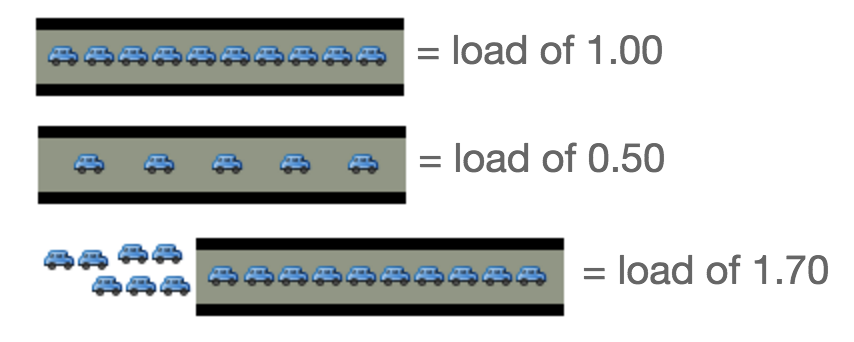
\includegraphics[width=0.55\textwidth]{images/car-analogy.png}
\end{center}

Being at or above 1.00 isn't necessarily bad, but you should be concerned if there is consistent load of 1.00 or above. And if you are below 1.00 but getting close to it, you know how much room you have to scale things up -- if load is 0.4 you can increase handily. If load is 0.9 you're pushing the limit already. If load is above 0.70 then it's probably time to investigate. If it's at 1.00 consistently we have a serious problem. If it's up to 5.00 then this is a red alert situation.

Now this is for a single CPU -- if you have a load of 3.00 and a quad core CPU, this is okay. You have, in the traffic analogy, four lanes of traffic, of which 3 are being used to capacity. So we have a fourth lane free and it's as if we're at 75\% utilization on a single CPU.


Back to our example. Is it CPU? The Application Server CPU utilization, on average, was about 10\% and on the database server, about 36\%. So that is probably not the cause. 

Next on the list is memory. One way to tell if memory is the limiting factor is actually to look at disk utilization. If there is not enough RAM in the box, there will be swapping and then performance goes out the window and scalability goes with. That is of course, the worst case. You can ask via \texttt{top} about how much swap is being used, but that's probably not the interesting value. 

\begin{verbatim}
KiB Mem:   8167736 total,  6754408 used,  1413328 free,   172256 buffers
KiB Swap:  8378364 total,  1313972 used,  7064392 free.  2084336 cached Mem
\end{verbatim}

This can be misleading though, because memory being ``full'' does not necessarily mean anything bad. It means the resource is being used to its maximum potential, yes, but there is no benefit to keeping a block of memory open for no reason. Things will move into and out of memory as they need to, and nobody hands out medals to indicate that you did an awesome job of keeping free memory. It's not like going under budget in your department for the year.  Also, memory is not like the CPU; if there's nothing for the CPU to do, it will just idle (or go to a low power state, which is nice for saving the planet). But memory won't ``forget'' data if it doesn't happen to be needed right now - data will hang around in memory until there is a reason to move or change it. So freaking out about memory appearing as full is kind of like getting all in a knot about how ``System Idle Process'' is hammering the CPU\footnote{Yes, a tech journalist named John Dvorak really wrote an article about this, and I will never, ever forgive him for it.}.

You can also ask about page faults, with the command \texttt{ps -eo min\_flt,maj\_flt,cmd} which will give you the major page faults (had to fetch from disk) and minor page faults (had to copy a page from another process). The output of this is too big even for the notes, but try it yourself (or I might be able to do a demo of it in class). But this is lifetime and you could have a trillion page faults at the beginning of your program and then after that everything is fine. What you really want is to ask Linux for a report on swapping:

\begin{verbatim}
jz@Loki:~$ vmstat 5
procs -----------memory---------- ---swap-- -----io---- -system-- ------cpu-----
 r  b   swpd   free   buff  cache   si   so    bi    bo   in   cs us sy id wa st
 1  0 1313972 1414600 172232 2084296    0    0     3    39    1    1 27  1 72  0  0
 0  0 1313972 1414476 172232 2084296    0    0     0    21  359  735 19  0 80  0  0
 0  0 1313972 1414656 172236 2084228    0    0     0   102  388  758 22  0 78  0  0
 4  0 1313972 1414592 172240 2084292    0    0     0    16  501  847 33  0 67  0  0
 0  0 1313972 1412028 172240 2084296    0    0     0     0  459  814 29  0 71  0  0
\end{verbatim}

In particular, the columns ``si'' (swap in) and ``so'' (swap out) are the ones to pay attention to. In the above example, they are all zero. That is excellent and tends to indicate that we are not swapping to disk and that's not the performance limiting factor. Sometimes we don't get that situation. A little bit of swapping may be inevitable, but if we have lots of swapping, we have a very big problem. Here's a not-so-nice example, from~\cite{vmstat}:

\begin{verbatim}
  procs                      memory    swap          io     system cpu
r  b  w   swpd   free  buff cache  si  so   bi   bo   in    cs us  sy  id
. . .
1  0  0  13344   1444  1308 19692   0 168  129   42 1505   713 20  11  69
1  0  0  13856   1640  1308 18524  64 516  379  129 4341   646 24  34  42
3  0  0  13856   1084  1308 18316  56  64   14    0  320  1022 84   9   8
\end{verbatim}

If we're not doing significant swapping, then memory isn't holding us back, so we can conclude it is not the limiting factor in scaling the application up. On to disk.

Looking at disk might seem slightly redundant if memory is not the limiting factor. After all, if the data were in memory it would be unnecessary to go to disk in the first place. Still, sometimes we can take a look at the disk and see if that is our bottleneck.

{\scriptsize
\begin{verbatim}
jz@Loki:~$ iostat -dx /dev/sda 5 
Linux 3.13.0-24-generic (Loki) 	16-02-13 	_x86_64_	(4 CPU)

Device:         rrqm/s   wrqm/s     r/s     w/s    rkB/s    wkB/s avgrq-sz avgqu-sz   await r_await w_await  svctm  %util
sda               0.24     2.78    0.45    2.40    11.60   154.98   116.91     0.17   61.07   11.57   70.27   4.70   1.34
\end{verbatim}
}

It's that last column, \%util that tells us what we want to know. The device bandwidth here is barely being used at all. If you saw it up at 100\% then you would know that the disk was being maxed out and that would be a pretty obvious indicator that it is the limiting factor. This does not tell you much about what is using the CPU, of course, and you can look at what processes are using the I/O subsystems with \texttt{iotop} which requires root privileges\footnote{https://xkcd.com/149/}.

That leaves us with networks. We can ask about the network with \texttt{nload}: which gives the current, average, min, max, and total values. And you get a nice little graph if there is anything to see. It's not so much fun if nothing is happening. But you'll get the summary, at least:

\begin{verbatim}
Curr: 3.32 kBit/s
Avg: 2.95 kBit/s
Min: 1.02 kBit/s
Max: 12.60 kBit/s
Ttl: 39.76 GByte                                                                                       \end{verbatim}


So, back to the original question. The book contains the full story, which is maybe interesting to you if you wanted to dig into the specifics about Oracle 10g and SQL query syntax. I speculate that you do not care about the details, but 96.4\% of the total database call time was attributed to database CPU, so let's look at the database queries themselves. Sure enough, the ``top 5'' queries were taking up a huge amount of time and they all look something like:

\begin{verbatim}
SELECT documentId, classId, dataGroupId, consistencyId FROM objectTable WHERE objectID = <value>;
\end{verbatim}

Why does performance of this stink? Well, because we're doing a lot of reads from the database. The reads themselves don't necessarily go to disk (cache/buffers/etc may save us here) but we're still doing a lot of reads of data. To speed this up, what we need is to add an additional index for each of these tables. 

This is one of the strategies we've talked about before -- ``be prepared''. If we know that the operation like the one above is going to be a common one, then we can tell the SQL server this and have it be prepared for that by defining an index. Some additional work is done to prepare the index and to maintain it when the data in the table is modified, but it makes the query a lot faster when it does come. 

And sure enough, we can see the result~\cite{swps}:

\begin{center}
	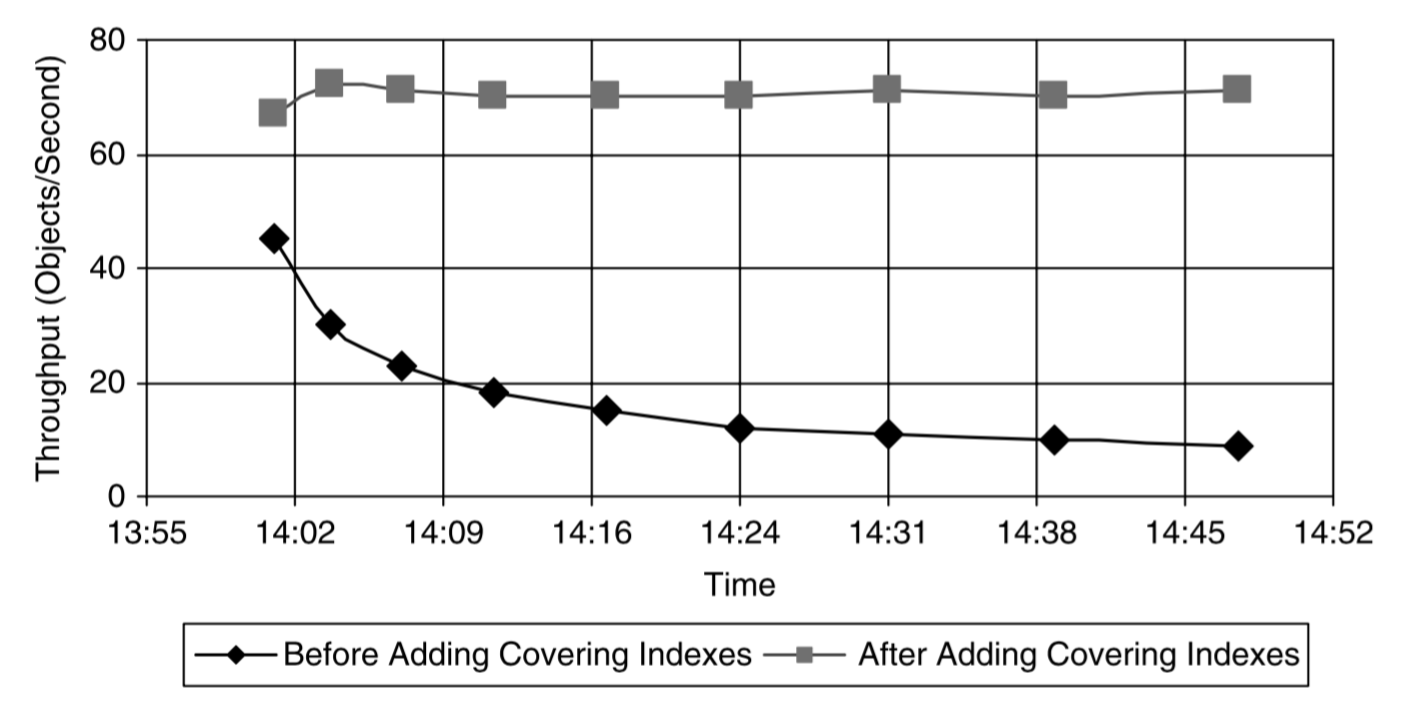
\includegraphics[width=0.85\textwidth]{images/adding-indexes.png}
\end{center}










\chapter*{31 --- Introduction to Queueing Theory}

\addcontentsline{toc}{chapter}{31 --- Introduction to Queueing Theory}

\section*{A Short Introduction to Queueing Theory}

Queueing theory is literally the theory of queues---what makes queues appear, how will they behave, and how do we make them go away? Queueing theory has played a role in your life whether you know it or not: this is how tech support at Rogers or Bell or Telus or whomever decides just how many customer service agents to have available at any given time. Of course, your local telecom chooses to minimize the number of employees at the cost of making you wait (``Your call is important to us; please hold while we ignore it.'') but they study carefully how much waiting is too much waiting and how much is too little. Queueing theory is applicable to lots of fields, including industrial design, call centres, telecom systems, and computers executing transactions. 

To scale up a system, we have a lot of choices to make, and these will work best if they are supported by data. Queueing theory helps us decide what's best. Here are a few possible examples, from~\cite{pmd}:

\begin{itemize}
 \item Given a choice between a single machine with speed $s$ or $n$ machines, each with speed $s/n$, which should we choose?
 \item If the arrival rate and service rate double, how does the mean response time change?
 \item Should we try to balance load or is that a waste of time/effort?
 \item Can we give priority to certain operations without harming another category of job?
 \item How do job size variability and heavy-tailed workloads affect our choices of scheduling policy?
 \item If 12 servers is enough to handle 9 jobs per second, do we need 12~000 servers if we have an arrival rate if 9~000 jobs per second?
\end{itemize}

I tend to tell stories about banks that imply I hate them. Not really, they're just a place where there's likely to be a queue and I'm likely to be annoyed and thinking about how to optimize this situation. So let's define some terms formally, to make sure we're all on the same page when it comes to terminology and language. Some of these will seem obvious, but let's be complete (like the book~\cite{swps}):

\begin{itemize}
	\item Server - The banking centre fulfilling customer requests.
	\item Customer - Initiator of service requests.
	\item Wait time - The time a customer spends waiting in line.
	\item Service time - The time from when a teller starts to serve a customer up to the time when the next customer is called forward.
	\item Arrival rate - The rate at which customers arrive.
	\item Service rate - the rate at which customer requests are serviced.
	\item Utilization - The fraction of the teller's time used actually handling customer requests (not idling).
	\item Queue length - The total number of customers waiting, or currently with a teller, or both.
	\item Response time - The sum of wait and service time for a single visit.
	\item Residence time - The total response time if a customer visits several tellers (or the same one multiple times).
	\item Throughput - The rate at which customers get their requests serviced and dealt with.
\end{itemize}

The mathematical symbols for this are represented in the following table~\cite{swps}:


\begin{center}
	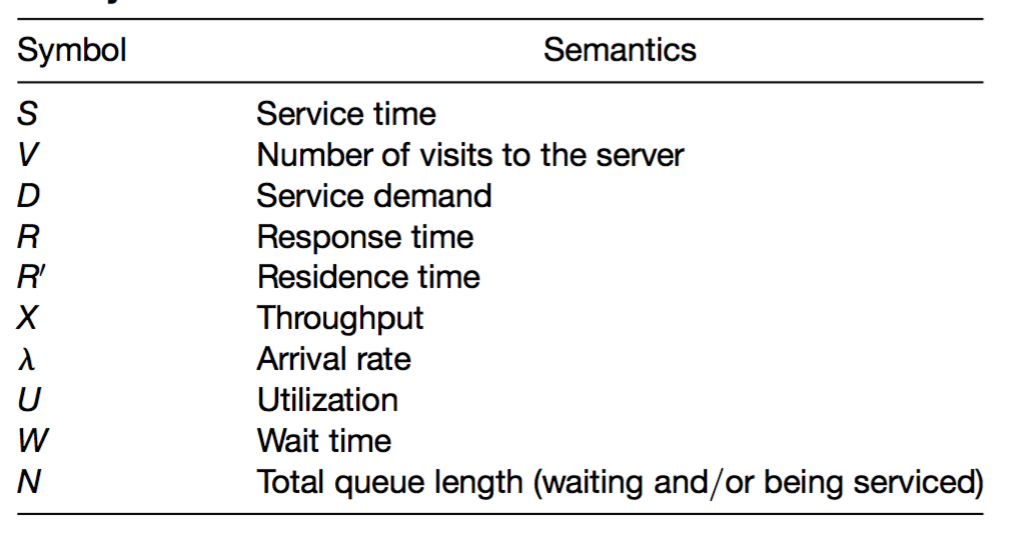
\includegraphics[width=0.65\textwidth]{images/math-symbols.png}
\end{center}

If you're cynical like me, you will think the bank works very hard to not have tellers in the bank to maximize your wait time and minimize their staffing costs. It's actually (allegedly) a trade-off: if I have to wait too long to do my banking, I could always take my business elsewhere (but is that likely to happen?). Minimizing customer wait time makes customers happy, so that's something the bank should want. It would also be nice if the bank trains its tellers well, so they can complete all operations, even unusual ones, quickly and efficiently, reducing the service time. The bank is not a charity operation so they will of course want to minimize staffing, but it knows that overstaffed is bad and understaffed is also bad. 

Back to the realm of computers: you have lots of queues in your computer. The CPU uses a time-sharing scheduler to run as many concurrent programs as possible. A router has a queue for packets (data) that has a maximum size, and if this is exceeded, packets will be simply dropped. 

Queueing theory gives us a formal framework with which to grapple with our problems instead of just guessing. Remember how bad we are at guessing. 


\paragraph{Example.} Let's look at a simple example from~\cite{pmd}. Imagine we have a system with one CPU that serves a queue of jobs in First-Come-First-Served (FCFS) order with an arrival rate $\lambda$ of 3 jobs per second. Each job takes some amount of time and resources, but we can ignore the particulars for right now. Suppose the average service rate $\mu$ is 5 jobs per second (or stated another way, the average job requires $0.2s$ to service). The system is not overloaded: 3 jobs per second arriving is less than 5 jobs per second being serviced. Our terminology for describing the mean response time will be $E[T]$. 


Suppose now that your boss says that tomorrow the arrival rate will double. If you do nothing, you can imagine, there will be a problem: we would have 6 jobs arriving per second, on average, to a system that can service, on average, 5 jobs per second. You have been allocated some budget to replace the CPU with a faster one, and you should choose one so that the jobs still have a mean response time of $E[T]$. This situation is depicted below~\cite{pmd}:


\begin{center}
	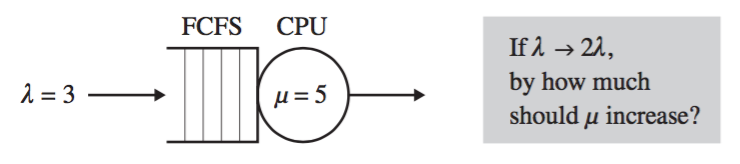
\includegraphics[width=0.5\textwidth]{images/qt-example1.png}
\end{center}

That is, customers should not notice the increase in arrival rate. So, should we (1) double the CPU speed; (2) more than double the CPU speed; or (3) less than double the CPU speed?

The answer is (3): we don't need to double the CPU speed. We can see later in formal terms why this is the case, but think for a minute about why it is? If we double the service rate and double the arrival rate, we actually get half the mean response time...

\paragraph{Example 2.} Okay, how about another example from~\cite{pmd}. There are always $N=6$ jobs running at a time. As soon as a job completes, a new one is started (this is called a \textit{closed system}). Each job goes through to be processed on one of two servers (and it is 50-50 where the job ends up), each of which has a service time $\mu$ of 1 job per 3 seconds. Again, depicted below~\cite{pmd}:


\begin{center}
	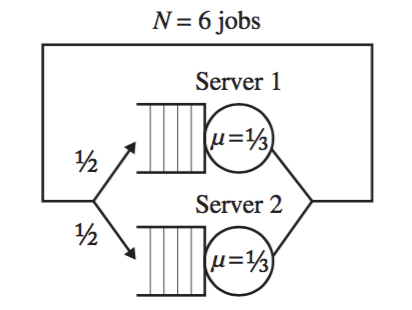
\includegraphics[width=0.3\textwidth]{images/qt-example2.png}
\end{center}

Bad news: sometimes, improvements do nothing. If we replace server one which is twice as fast (so 2 jobs per 3 seconds), does that help? Nope. Not really. Does raising $N$ help? Nope, negligible effect. The bottleneck device is the limiting factor. Strangely, dropping $N$ to 1 means the server replacement makes a difference, if you can call that improvement. 

What if it's an \textit{open system} where arrival times are independent of completion, as below~\cite{pmd}?


\begin{center}
	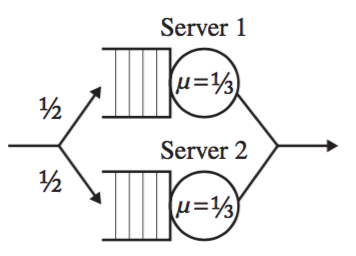
\includegraphics[width=0.3\textwidth]{images/qt-example2-2.png}
\end{center}

In this case, yes, replacing server 1 makes a huge difference!

\paragraph{Example 3.} A third example, this time addressing directly the question of do we want one fast server or $n$ slower ones? Horse-sized duck and duck-sized horses jokes aside, what is better if we want to minimize the mean response time when we have non-preemptable jobs (i.e., once started, a job has to run to completion and cannot be interrupted)~\cite{pmd}:


\begin{center}
	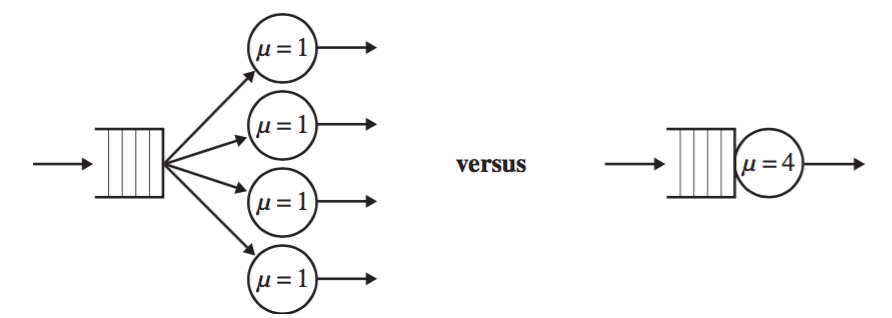
\includegraphics[width=0.6\textwidth]{images/qt-example3.png}
\end{center}

The answer is ``it depends''. That's frustrating, but this is Sparta. Or at least, real life. One big factor is the variability of the job sizes. Imagine you are at the grocery store and most people have 12 items or fewer\footnote{Not less. Fewer. It is countable; therefore fewer. Yes, I am obsessive about this.} and there's one guy who's buying 85 items. You don't want to be standing in line with milk and eggs behind someone who is trying to buy six of everything, do you? So if there's high variability, you probably want multiple servers -- the guy buying the whole store can hold up line \#1 and you can go to line \#4 and you're out and done before he is finished.

What if the load is low? Chances are you would prefer the one fast server instead of having some number of servers doing nothing.

What if jobs are interruptible (preemptible)? You could always use a single fast machine to simulate $n$ slow machines, so a single fast machine is at least as good as the alternative. 

\subsection*{A Digression on Load Balancing}

Imagine your typical ``server farm'' - you have $n$ servers that are all responsible for handling incoming requests. Let's imagine all servers are the same (or close enough). What we typically see in load balancing is assignment of tasks to servers via some dispatcher~\cite{pmd}:

\begin{center}
	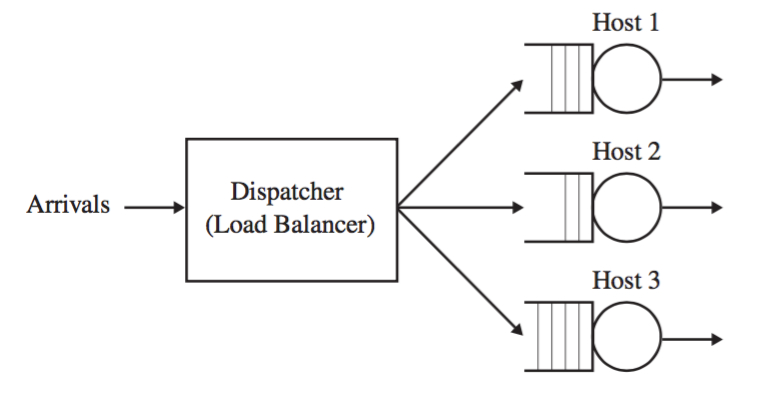
\includegraphics[width=0.6\textwidth]{images/central-dispatcher.png}
\end{center}

This isn't the only kind of load balancing we can do; there is also the ability to do after-the-fact assignment (or work-stealing), which consists of monitoring the various queues and reassigning work if it's piling up somewhere.

There are a few different task assignment policies---ways in which we can assign work to servers~\cite{pmd}:

\begin{itemize}
	\item Random: Exactly what it sounds like.
	\item Round-Robin: The $i$th job goes to host $i$ modulo $n$.
	\item Shortest-Queue: The job goes to the server with the shortest queue.
	\item Size-Interval-Task-Assignment: Short jobs go to one server, medium to another, long to another...
	\item Least-Work-Left: A job goes to the server that has the least total remaining work, where work is the sum of the size of the jobs.
	\item Central-Queue: Rather than being assigned to a host directly, when a server needs work to do, it gets the first job in the central queue.
\end{itemize}

Which of these policies yields the lowest mean response time? Answer: truthfully, nobody knows. It depends, of course, on your job variability and and that sort of thing, but it hasn't been well studied. PhD, anyone?

\subsection*{Red Line Overload\footnote{You've seen ``Top Gun'', right? \url{https://www.youtube.com/watch?v=siwpn14IE7E}}}

Earlier I mentioned it would probably be bad to see 6 jobs arriving per second to a system that can handle 5 per second. This doesn't seem like rocket science, but it bears repeating. In our discussion we require that $\lambda \leq \mu$ and assume that $\lambda < \mu$. That is to say, we are not overloaded (as engineering students you may be amused by the idea that you might one day NOT be overloaded). Remember now that the values for $\lambda$ and $\mu$ are averages, so it could happen that temporarily we ``fall behind'' a bit, but then make up for it a little later on, or we temporarily get ahead before a bunch more work gets piled on. Think about the long term, though -- if we are not at least keeping up then this will eventually get out of hand. How badly? Well, in the limit, the queue length goes to infinity.

The justification comes from~\cite{pmd}: Let's represent time with $t$, its usual symbol and define $N(t)$ as the number of jobs in the system at time $t$. $A(t)$ represents arrivals by time $t$ and $D(t)$ represents departures by time $t$. So:

\begin{center}
	$E[N(t)] = E[A(t)] - E[D(t)] \geq \lambda t - \mu t = t (\lambda - \mu) $
\end{center}

The tiniest bit of calculus says that if arrivals exceed departures, taking the limit as $t$ goes to infinity means $t (\lambda - \mu) $ also goes to infinity. Whoops. So to prevent this terrible situation we just happily assume that this doesn't happen\footnote{I'm reminded of a funny engineering saying that says if you encounter a system that is nonlinear, you can decide that nonlinear systems are too difficult to reason about, assume the system is linear, and proceed.}. 

Raising $\mu$ is generally desirable. This is, after all, programming for performance -- the faster we complete work, the more work we can get done in the same amount of time. Improving the service rate, however, does not necessarily improve the throughput. 

Wait, what? We've assumed that the arrival rate is less than the service rate. So we have enough capacity to handle all incoming work. So the limiting factor on completed work is actually arriving work. We have the capacity to do at least what is arriving and possibly a bit more. Adding more work capacity doesn't mean more work gets done if there isn't any more work to do. You might be capable of completing six assignments for this class in a term, but if you're (mercifully) only assigned four, then you will only complete four. So raising $\mu$ increases the maximum possible throughput, but does not necessarily increase the actual throughput.

But just to make you suffer, things are very different in a closed system: one in which there is always more work to do and as soon as one item is finished the next one enters the queue. This is the case in batch systems. You know, the old mainframe kind of processing where you submit your job to be run overnight and in the morning you get a result. Hopefully the one you wanted. In that case, we are running at capacity all the time, so actually $\mu$ is the controlling factor -- the throughput is exactly the service rate. 

Not that open networks are particularly intuitive, but closed networks can kind of mess with our intuition in general. Imagine we have a closed system with Multiprogramming Level (MPL) of $N$ as below~\cite{pmd}:

\begin{center}
	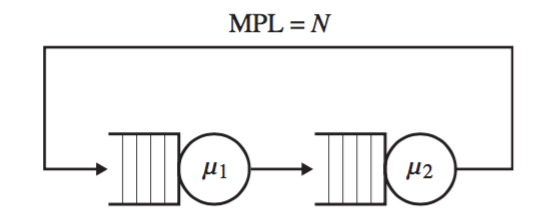
\includegraphics[width=0.4\textwidth]{images/tandem-closed.png}
\end{center}

What is the throughput here? Intuition suggests min($\mu_{1}, \mu_{2}$), right? Sometimes. This is okay if the slower server is always busy, but that's not always the case. What if $N$ is 1? Okay, that's a bit of an exception case though. What about $N$ being 2? Then the slower server has some work to do at all times right? Nope, sadly not. Sometimes the slow server is faster than the fast server, because $\mu_{1}$ and $\mu_{2}$ are just averages. And averages can be misleading! The average family might have 2.3 children (or whatever the figure is), but you can't exactly have 0.3 of a child...

\subsection*{Don't Guess...}
One final anecdote from~\cite{pmd} on the subject of measuring $\mu$. Some smart folks at IBM wanted to know, given the arrival rate $\lambda$, what the mean job size, $E[S]$ (which is $1/\mu$) was. Well, $E[S]$ is the mean time required for a job in isolation, so our experiment should be a hundred runs of sending a single job into the system and averaging the values. This is okay, but does not reflect reality where we have things like caching of data and multiple concurrent jobs. There are two basic strategies we can follow, depending on whether it is an open or closed system for getting a value for $\mu$, allowing simple computation of $E[S]$.

The open system strategy is: ramp up $\lambda$. Keep piling more jobs on the system. At some point the system will not be able to keep up. Once the completion rate levels off, we hit the limit and we have a value for $\mu$.

The closed system strategy: set it up so there is always work to do. In closed systems, there's often consideration given to \textit{think time} -- this is what happens when the user is on the command line and dispatching work to do. The user sends a command and awaits a result. After the result, some time passes while the user decides what to do next (or does code editing before running the compiler again). To keep the system totally busy in the stress test, we need think time to be zero -- so additional work is always available. And then we can simply measure the jobs completing per second, giving us $\mu$ directly.




practical queueing theory:  https://www.youtube.com/watch?v=IPxBKxU8GIQ





\chapter*{32 --- Probability, Convergence, \& Ergodicity}

\addcontentsline{toc}{chapter}{32 --- Probability, Convergence, \& Ergodicity}

\section*{A Comically Short Review of Probability}

So as a quick preface -- to understand some of this material you would be well served to have some familiarity with this subject. I imagine you took a course on probability earlier, but perhaps this material is not exactly fresh in your mind. That being the case, a review of the subject by reading, say~\cite{swps,pmd} will help. But let's go over some of it, in brief. 

Suppose we are doing an experiment like rolling dice (a favourite of statistics profs everywhere). We associate the outcomes of these experiments with is called a random variable. A random variable $X$ has many instances, each with some probability; if you roll a fair die $X$ can have instances of ${1, 2, 3, 4, 5, 6}$, each with a probability of $1/6$ (because we defined this die to be perfectly fair). In a die roll, the events (values of the roll) are discrete - you can't roll 2.1 or 5.5. Time is generally modelled as continuous, but in reality there are limits to how accurately we can measure time on a computer. The resolution depends on the hardware. 

Building on this, we can think of the outcome of an experiment as an ``event''. Probability theory loves to talk about events. We can ask ourselves all kinds of questions like: what is the probability of rolling four 1s on a 20-sided-die in a row\footnote{I played a dwarf warrior in D\&D, although truthfully Shadowrun was always much more my style. Elven decker!}? Looking at this from the perspective of application programmers, we say the number of users at time $t$ can be represented by a random variable $U$ and then we can ask ourselves what is the probability of $U$ being greater than 1000?

Probability is usually defined as some sort of experiment with a sample space $\Omega$ and some subset of this $E$ is an \textit{event}. A standard example: you have a perfectly fair coin. Possible outcomes are heads, tails, and very rarely, edge (look, it could happen). Each outcome is an event with a certain probability -- i.e., chance of happening -- usually written $P\{E_{n}\}$.

If the coin coming up heads is an event $E_{1}$ and it coming up tails $E_{2}$ are these independent? No, they are not. They are mutually exclusive - if the coin comes up heads it cannot possibly also come up tails. Events are sets and we can do unions and intersections and such. The formal definition of mutual exclusivity is $E_{1} \cap E_{2} = \emptyset$. Independence, on the other hand, means the probability of $E_{1}$ does not change if event $E_{2}$ has occurred.

Conditional probability is also important: what is the probability of event $E$ given that event $F$ has occurred? The notation is $P\{ E~|~F \}$ and it has a definition (as long as $P\{F\}$ is not zero): 

\begin{center}
	$P\{E~|~F\} = \dfrac{P\{E \cap F\}}{P\{F\}}$
\end{center}

If events $E$ and $F$ are independent, then $P\{E \cap F\}$ is equal to $P\{E\} \cdot P\{F\}$. That is, the probability of $E$ is not affected by the occurrence of $F$. Suppose you flip a coin four times and it comes up heads each time (event $F$). What is the probability that the next coin flip will be tails (event $E$)? Sadly, a lot of people think that after four heads, now tails is ``due'' and the chance of it being tails is higher than the usual 50-50 (minus the edge case). This is not true -- the next coin flip is independent of all the coin flips that went before it.

A statistics professor would probably come knock down my door and give me a savage beating if I also did not mention Bayes Law. If we want $P\{ F~|~E \}$, but have $P\{ E~|~F \}$ can we get it? Yes, if we know $P\{F\}$ and $P\{E\}$. Bayes law is:

\begin{center}
	$P\{F~|~E\} = \dfrac{P\{E~|~F\} \cdot P\{F\}}{P\{E\}}$
\end{center}

For now let us focus on discrete random variables (i.e., those with a countable number of values). For a random variable $X$ we can define a probability mass function (p.m.f.);

\begin{center}
	$p_{x}(a) = P \{ X = a \},$ where $\sum\limits_{x}^{~} p_{x}(x) = 1$
\end{center}
	and the cumulative distribution function is:
\begin{center}
	$F_{x}(a) = P \{ X \leq a \} = \sum\limits_{x \leq a} p_{x}(x)$
\end{center}

There are five distributions we want to discuss: Bernoulli, Binomial, Geometric, Poisson, and Exponential. The Poisson distribution is the one to focus on, but let's not overlook anything important.

Bernoulli represents a coin flip: so the coin has a probability $p$ of coming up heads and $1-p$ of coming up tails. So the random variable $X$ associated evaluates to 1 (heads) with probability $p$ and 0 (tails) with probability $1-p$. Thus the p.m.f. is $p_{x}(1) = p$ and $p_{x}(0) = 1 - p$. 

The Binomial distribution builds upon the Bernoulli distribution. A coin with probability $p$ of coming up heads flipped $n$ times (assuming coin flips are independent). The random variable $X$ if it's Binomial, represents the number of heads when flipping a Bernoulli coin $n$ times. So $X$ can take on values of $\{0, 1, \ldots, n\}$. 

The Geometric distribution builds on Bernoulli. Again suppose we have the coin with probability $p$ of coming up heads. If we want to ask how many (independent) coin flips it will take until it comes up heads, the Geometric distribution answers this question. $X$ is the number of flips until we get the result we want.

Applying this to the realm of computing, as in~\cite{pmd}. Suppose we have a server farm that has $n$ disks, each of which independently dies (fails) with probability $p$ in a year. So what is the appropriate model for each of these questions?

\begin{enumerate}
	\item How many disks die in the first year?
	\item Given disk $d$, how long until this disk dies?
	\item After one year, is a specific disk $d$ alive or dead?
\end{enumerate}

The answers are (1) Binomial, (2) Geometric, and (3) Bernoulli.

Now let us turn to the Poisson distribution; this is very common in computing. This is our somewhat ``natural'' idea of randomness. This distribution arises when we have a mixture of a very large number of sources, each with a very small probability. So this is a lot like the number of arrivals to a website or packets at a router in some unit time. If a random variable $X$ has a Poisson distribution, the p.m.f. is:

\[
	p_{x}(i) = \dfrac{e^{-\lambda}\lambda^{i}}{i!},\mbox{ where $i = 0, 1, 2\ldots$}.
\]

One more thing: there are also continuous random variables, and although we won't talk much about them, we should also consider the exponential distribution. This is a distribution where the probability density function (p.m.f.) drops off exponentially. If $x \geq 0$, then $f_{x}(x) = \lambda e^{-\lambda x})$. The cumulative distribution function, i.e., $F_{x}(x) = P\{ X \leq x \}$ is the integration of this function from negative infinity to $x$, equal to $1-e^{-\lambda x}$ (again, for $x \geq 0$). What we care about here is actually the inverse of this, $\overline{F_{x}}(x)$, the probability that the value is greater than $x$ -- namely, the outliers or the ``tail'' of the distribution. Note that we see a constant drop-off of $e^{-\lambda}$ with each unit increase of $x$. Heavy tails are not very nice. 


How about expectation and variance. Recall the notation here $E[X]$ is the expected value of a random variable $X$. Expected value is, not kidding, just a ``weighted average''\footnote{One of the biggest light bulb moments of my undergraduate life.}. Let's say you're entering into a game where you pay \$3 to play. If you have a 50\% chance of losing all your money, a 10\% chance of winning \$10, and a 40\% chance of getting your \$3 back, should you play?

Do the math: your expected return is $(0.5 \times 0) + (0.1 \times 10) + (0.4 \times 3) \rightarrow 0 + 1 + 1.2 = 2.2$. So you expect that by playing this game, for every \$3 entry, you get back \$2.20 (on average). It doesn't seem like a good investment, does it? Econ 101 logic would tell you the answer is: how much do you value the fun of playing and the hope and excitement of winning? If it's equal to or more than \$0.80 then it is worth it.

Proofs of these exist in the textbook(s) but let's not belabour the point by proving it. Just take my word for it that the expectation for a Geometric distribution with probability $p$ is $1/p$: so if we have a coin where the probability of landing heads is $1/3$, then we expect it takes 3 flips to get heads. If a Poisson distribution applies to something, the expectation $E[\lambda] = \lambda$. Okay, that's nice.

The weighted average is nice, but it's not the whole story. If your numbers are 5, 6, and 7, then their average is 6. But the average of the numbers 0, 6, and 12 is also 6. But we should know already that averages can be misleading. A student who takes six courses in a term is unlikely to find that these six exams are distributed equally over the three week exam period as 2, 2, and 2, with at least a little time between any two exams. On the contrary, said student may find there are four in the first week, then a long pause before the next, or two back to back, or even two at once. This student might think the registrar's office hates him or her, but rest assured, it is nothing personal. An average arrival rate of 1 request per second could still, with some probability, produce 3 arrivals in a single second. These should illustrate the idea that we can have an average that seems benign but have outlier situations that are actually messy to deal with.

The formal definition of variance of a random variable $X$ is the expected squared difference of $X$ from its mean:

\[
	\mathrm{Var}(X) = E[X^{2}] - (E[X])^{2}
\]

Just take my word for it at the moment that the following table, copied from the book~\cite{pmd} is correct:

\begin{center}
\begin{tabular}{l|l|l}
	\textbf{Distribution} & \textbf{Mean} & \textbf{Variance}\\ \hline
	Bernoulli & $p$ & $p(1-p)$\\ \hline
	Binomial & $np$ & $np(1-p)$\\ \hline
	Geometric & $\dfrac{1}{p}$ & $\dfrac{1-p}{p^{2}}$ \\ \hline
	Poisson & $\lambda$ & $\lambda$
\end{tabular}
\end{center}

There is plenty more that you should know about (conditional probability, exponential distributions, etc.) but let us break off this thrilling review of probability and put it to use.

\section*{Convergence}

Think back to calculus class. Remember when we talk about limits: $\lim_{x\to\infty} f(x)$. There is an answer for this if the function does (somehow) converge on some value, such as the function $f(x) = 1/x^{2}$ converging to 0.

We would like to see that our random variables converge. You might flip a coin four times and all four times it comes up heads. That doesn't match our expectation that we should have about half heads and half tails. We have convergence if, given enough samples and enough sample paths, it will converge to the 0.5 we expect. There may be some sample paths that don't converge (e.g., continually coming up heads), but they have a ``probability mass'' of zero (i.e., they are incredibly unlikely).  There are in fact uncountably many ``bad paths'', each with probability zero (but that's okay). Zero probability doesn't mean it can't happen, mind you.

An image of what convergence looks like~\cite{pmd}:

\begin{center}
	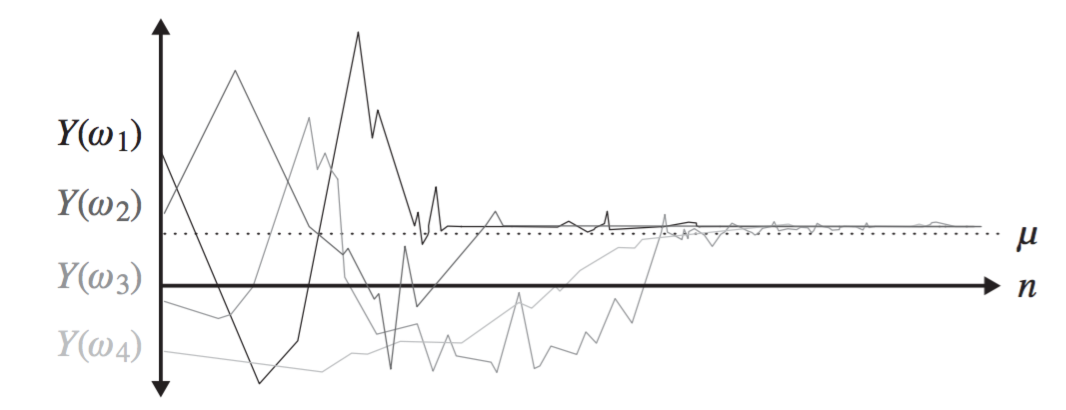
\includegraphics[width=0.6\textwidth]{images/convergence.png}
\end{center}

We won't concern ourselves with systems where there is no convergence. We'll just deal with situations where there is a convergence. Almost every sample path (series of experiments) will eventually behave well if we take enough samples. That is, get past the initial conditions. But sampling is important in our discussion about scalability...

\section*{Tim and Enzo}
A small but important digression on the subject of sampling, measurement, and testing, from~\cite{pmd}. You have an idea of what an average is, but there are two different relevant types of average here---the time average and ensemble average. 

Let us just focus on having a single First-Come-First-Serve queue. Every second, a new job arrives with probability $p$ and if there is any work to do, the job being worked on is completed with probability $q$ (and $q > p$). As a definition, let $N(v)$ equal the number of jobs in the system at a time $v$. In the story, Tim and Enzo are trying to simulate the FCFS system to determine what is the average number of jobs in the system. 

Tim decides he's going to run it as one really long simulation. He simulates the queue over a very long period, logging as he goes, taking a million samples. Then he takes the average value over those samples to get the average number of jobs.

Enzo does something slightly different: instead of having one super long simulation, he does 1000 shorter simulations. He waits until the simulation has run for 1000 seconds and then samples the queue at exactly that point, obtaining one value. This experiment is restarted with a new random seed. So after obtaining a thousand samples, he averages these, and Enzo produces another average number of jobs.

A little illustration of Tim and Enzo from~\cite{pmd}:

\begin{center}
	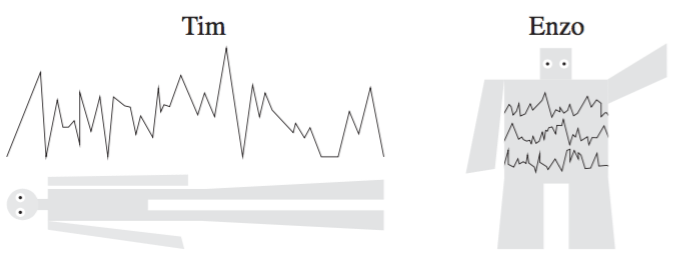
\includegraphics[width=0.5\textwidth]{images/timenzo.png}
\end{center}

So -- who has done this correctly, Tim or Enzo?

The time average has potential problems because we are only looking at a single sequence and maybe something very unusual has happened here in this single run. The ensemble average is more likely what we talk about when we talk about the system being at ``steady state'' (i.e., past the initial conditions). So we kind of like the Enzo approach. Plus, this is programming for performance (or as a student said, programming for parallelism) -- we can do 1000 simulations concurrently if we have enough CPU cores! Tim's approach still has some merit though.

A note about initial conditions: both the Tim and Enzo approaches here require caring about the initial conditions. Enzo needs to make sure that the initial conditions (startup costs etc) have attenuated before the measurement point. Tim needs to ensure that the initial conditions impact a sufficiently small portion of all his measurements.

But! If we have a nicely behaved system, the time average and the ensemble average are the same (so both Tim and Enzo can be correct). What is a nicely behaved system? The word for this is \textit{ergodic}. That probably did not help, so what is an ergodic system? It is a system that is positive recurrent, aperiodic, and irreducible.

\textit{Irreducibility} means a process should be able to get from one state to any other state (where state is the number of jobs in the system). This means the initial state of the system does not matter. So if we started at 0 jobs or 10 we could still get to any state in the system (jobs at 2 or 27)\ldots

\textit{Positive recurrence} means that given an irreducible system, any state $i$ is revisited infinitely often, and the time between visits to that state are finite. So we can define a certain state as being a ``restart''. The logical choice in the case of a queue or similar is the idea of the queue being empty. Every time the queue gets down to zero jobs, it's a ``restart'' of sorts. 

This is what makes Tim's view and Enzo's view potentially the same. A single long run (Tim's view) is just like a number of independent runs (Enzo's view). Every time we get down to zero jobs in the queue, it's a restart. 

The \textit{aperiodicity} condition is required for the ensemble average to make sense or exist. That is to say, the state of the system should not be related to the time; i.e., it is not the case that the system is in state 0 when $t$ is even and state 1 when $t$ is odd. Otherwise the way Enzo chooses to sample, i.e., $t = 1000$, is potentially going to skew the result.

A graphical illustration, also from~\cite{pmd}, that shows how the time average over a single long run can be considered a chain of restarts or ``renewals''.

\begin{center}
	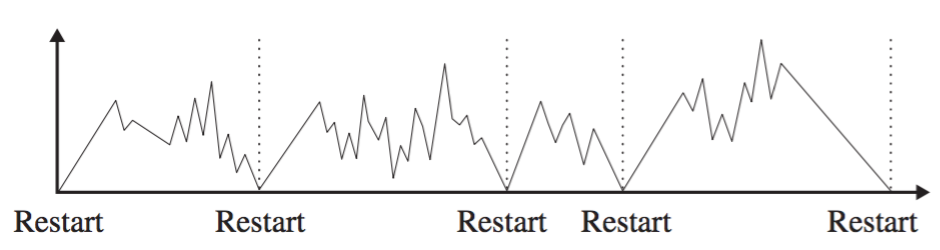
\includegraphics[width=0.5\textwidth]{images/systemrestart.png}
\end{center}

Both Tim and Enzo are correct for ergodic systems. Either method works to determine measurements and queueing theory values. Enzo's method has some advantages, e.g. parallelism and the ability to produce confidence intervals.

We've talked about the average number of jobs, but perhaps what we also care about is how long a job spends in the system, on average. We could compute either the time or ensemble average. 

\begin{center}
	Time Average = $\lim_{t\to\infty}\dfrac{\sum_{i=1}^{A(t)} T_{i}}{A(t)},$
\end{center}

where $A(t)$ is the number of arrivals by time $t$ and $T_{i}$ is the time in the system of arrival $i$. The average is taken over one sample path.

\begin{center}
	Ensemble Average = $\lim_{t\to\infty}E[T_{i}],$
\end{center}

where $E[T_{i}]$ is the average time in the system of job $i$, average being taken over all sample paths.









\chapter*{33 --- Applying Queueing Theory}

\addcontentsline{toc}{chapter}{33 --- Applying Queueing Theory}

The purpose of the examination in the recent lecture of probability is so that we could able to answer some interesting ``what if'' questions. So let's take a look at some of those, but first we'll stop to discuss Little's Law.

\section*{Little's Law}
Little's Law is a famous result, saying that the average number of jobs in the system equals the product of the average arrival rate into the system and the average time spent in the system. The source on this section is~\cite{pmd}.

\paragraph{Open Systems.} Let's start with an open system. Here is Little's Law, written more formally:

\[
	E[N] = \lambda E[T],
\]

where $E[N]$ is the expected value of the number of jobs in the system, $\lambda$ is the average arrival rate into the system, and $E[T]$ is the mean time jobs spend in the system. For example, if a University intakes an average of 5,000 students per year and each student spends an average of 4 years in school, then there are $4 \times 5000=20000$ students on average in the University~\cite{sigman-little-law}. The basic setup of Little's Law looks something like this~\cite{pmd}:

\begin{center}
	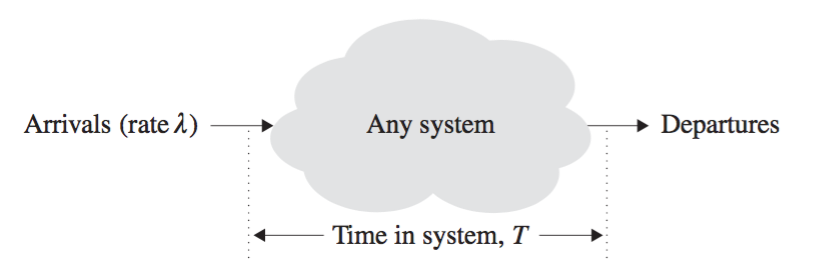
\includegraphics[width=0.5\textwidth]{images/littleslaw.png}
\end{center}

We don't need to know anything about the arrival process (Bernoulli, Poisson, etc\ldots), the service time distribution, network topology, etc. It seems intuitive that this is the case (or it should). Imagine a fast food restaurant: they make money by quick turnaround, so they get people out of the place quickly (low $E[T]$) and accordingly they don't require a lot of seating (low $E[N]$). A sit down restaurant is the opposite though; people leave slowly (high $E[T]$) and therefore the restaurant needs lots of seating (more $E[N]$). This example might seem weird from the perspective of the customer though---from your perspective, you may want to enjoy your evening---but the restaurant is eager to turn your table over, and get you out of there so a new set of guests can be seated. (Another way of looking at this is that restaurants are in the business of renting seats. It's not about food costs.)

If you prefer to think of this in a single FCFS queue version, imagine a customer arrives and sees $E[N]$ jobs ahead of her in the queue. The expected time for each customer to complete is $1/\lambda$, because the average rate of completions is $\lambda $. So we can approximate $E[T]$ as being roughly $\dfrac{1}{\lambda}E[N]$.

\paragraph{Closed Systems.} Remember that for closed systems, we have a rule that says there are $N$ jobs in process at any given time (the multiprocessing level of the system). If the system is ergodic, then $N = X \cdot E[T]$ where $N$ is the multiprogramming level, $X$ is the throughput rate, and $E[T]$ is the mean time jobs spend in the system. This assumes that there is zero think time, i.e., that jobs are always ready at once and don't have to wait for silly users.

If we do have to deal with the vagaries of users and think time, then we care more about the response time $E[R]$. So for a terminal-driven system, the expected response time is $E[R] = \dfrac{N}{X} - E[Z]$ where $N$ is the multiprogramming level, $X$ is the throughput, and $E[Z]$ is the mean time spent thinking. 

\section*{M/M/1}

Probabilistic processes are described according to their models, which will probably be one of the three~\cite{swps}:

\begin{enumerate}
	\item Deterministic (D) -- The process is predictable and characterized by constant factors. For example, the inter arrival times are constant (e.g., a task arrives every minute.)
	\item Markov (M) -- A memoryless process; the future states of the process are independent of the past history. The future state depends on only the present state.
	\item General (G) -- Completely arbitrary.
\end{enumerate}

We're going to focus on Markov processes, because they are nicer (and we have only limited time). It means that the number of arrivals follow the Poisson distribution; the inter-arrival times follow the exponential distribution, and service times follow the exponential distribution too. 

Those letters we saw are part of Kendall notation. It has six symbols, written in a specific order, separated by slashes. The order is $\alpha / \sigma / m / \beta / N / Q$. See the table below for the full explanation:

\begin{center}
\begin{tabular}{l|l} 
	\textbf{Symbol} & \textbf{Meaning} \\ \hline
	$\alpha$ & The type of distribution (Markov, General, Deterministic) \\ \hline
	$\sigma$ & The type of probability distribution for service time \\ \hline
	$m$ & Number of servers \\ \hline
	$\beta$ & Buffer size \\ \hline
	$N$ & Allowed population size (finite or infinite) \\ \hline
	$Q$ & Queueing policy \\ 
\end{tabular}
\end{center}

We often leave off the last three, assuming that there is an infinite buffer, infinite population, and a FIFO queueing policy. If that is the case, then we have only three values. Those three then produce the ``M/M/1'' and ``M/M/k'' symbols. ``M/M/1'' means a Markov arrival process, exponential queueing system, and a single server. When there are $k$ servers, of course the 1 is replaced with the $k$. These are the systems that we are going to examine.

We should also think about utilization, denoted $\rho$. It is a fraction between 0 and 1 and it is simply the amount of time that the server is busy. We talked about this earlier in an informal way, but now we can actually calculate it: $\rho = \lambda \times s$ (the arrival rate and service time). 

For M/M/1 systems, the completion time average $T_{q}$ is $\dfrac{s}{(1-\rho)}$ and the average length of the queue $W$ is $\dfrac{\rho^{2}}{1-\rho}$.

An example from~\cite{williams-q}: we have a server that completes a request, on average, in 10~ms. The time to complete a request is exponentially distributed. Over a period of 30 minutes, 117~000 jobs arrive. So this is a M/M/1 situation. How long did it take to complete the average request? What is the average length of the queue?

The service time $s$ is given as $0.01s$, the arrival rate is 65 requests per second. So we can calculate $\rho = 0.01 \times 65 = 0.65$. So we have what we need to plug and chug using the formul\ae\ from above to find the time to complete the average request is 28.6~ms and the average length of the queue is 1.21.

What about the number of jobs in the system? The value $Q$ gives the average number of jobs, including the waiting jobs and the ones being served. It is an average, of course. The probability that there are exactly $x$ jobs in the system at any time is given by the formula: $(1-\rho)\rho^{x}$. The probability that the number of jobs is less than or equal to $n$ is then given by: $\sum\limits_{i=0}^{n}(1-\rho)\rho^{i}$ (the sum of the probabilities of each of the numbers from 0 up to $n$). If you want to know the probability that there are more then $n$ at a time, then you can compute the sum from $n+1$ up to infinity. That might be unpleasant to calculate, but remember that probabilities sum to 1, so you can say that the probability of more than $n$ requests at once is simply $1 - \sum\limits_{i=0}^{n}(1-\rho)\rho^{i}$.

\section*{M/M/k}

Now let us take it to multiple servers. We will say jobs arrive at a single queue and then when a server is ready it will take the first job from the front of the queue. The servers are identical and jobs can be served by any server. So far, so simple.

Sadly, the math just got harder. Let's turn again to~\cite{williams-q} as the source for this section. The server utilization for the server farm is now $\rho = \lambda s / N$ (the average utilization for all $N$ servers). To make our calculations a little easier, we want an intermediate value $K$ which looks scary, but is not so bad:

\[ K = \cfrac{\sum_{i=0}^{N-1}\dfrac{(\lambda s)^{i}}{i!}}{{\sum_{i=0}^{N}\dfrac{(\lambda s)^{i}}{i!}}}.
\]

The first term, $i = 0$, is always 1. The denominator is always larger than the numerator, so $K$ is always less than 1. $K$ has no intrinsic meaning, it is just a a computational shorthand so the other formul\ae\  are not so messy.

What is the probability that all servers are busy? We represent this as $C$, the probability a new job will have to wait in the queue.

\[C = \cfrac{1 - K}{1 - \dfrac{\lambda s K}{N}}.\]

The M/M/k formul\ae, then, for the average completion time and average length of the queue are:

\[
  T_{q} = \dfrac{C s}{k(1 - \rho)} + s \mbox{ \qquad\qquad and \qquad\qquad } W = C \dfrac{\rho}{1 - \rho}.
\]

Let's do an example. Suppose we have a printer that can complete an average print job in two minutes. Every 2.5 minutes, a user submits a job to the printer. How long does it take to get the print job on average? We're starting with a single printer, so the system is M/M/1. Service time $s$ is 2 minutes; the arrival rate $\lambda$ is $1/2.5 = 0.4$. So $\rho = \lambda \times s = 0.4 \times 2 = 0.8$. So $T_{q} = s / (1 - \rho ) = 2 / (1 -0.8 ) = 10$. Ten minutes to get the print job. Ouch.

Here we have an opportunity to use the predictive power of queueing theory. Management is convinced that ten minute waits for print jobs is unreasonable, so we have been asked to decide what to do: should we buy a second printer of the same speed, or should we sell the old one and buy a printer that is double the speed?

The faster printer calculation is easy enough. Now $s = 1.0$ and $\lambda$ remains $0.4$, making $\rho = 0.4$. So rerunning the calculation: $T_{q} = s / (1 - \rho ) = 1 / (1 - 0.4 ) = 1.67$. 1:40 is a lot less time than 10:00! 

The two printer solution is more complicated. So let us calculate $K$ as the intermediate value. 

\[K = \cfrac{\sum_{i=0}^{N-1}\dfrac{(\lambda s)^{i}}{i!}}{{\sum_{i=0}^{N}\dfrac{(\lambda s)^{i}}{i!}}} = \cfrac{\dfrac{(\lambda s)^{0}}{0!} + \dfrac{(\lambda s)^{1}}{1!}}{\dfrac{(\lambda s)^{0}}{0!} + \dfrac{(\lambda s)^{1}}{1!} + \dfrac{(\lambda s)^{2}}{2!}} = 0.849057.\]

Now we can calculate $C$ as 0.22857 and $T_{q}$ as 2.57 minutes (by simple plug and chug calculations given the formul\ae\  above). Two observations jump out at us: (1) we doubled the number of printers, but now jobs are completed almost four times faster; and (2) the single fast printer is better, if utilization is low.

That is an important condition: if utilization is low. At some point will the two printers be a better choice than the single fast one? What if both printers are used to the max (100\% load)\ldots?

\section*{Queuing for Performance}

The plan is to take queueing theory and apply it in a performance model. The guide to this section is~\cite{williams-perf}. The basic process is:

\begin{enumerate}[noitemsep]
	\item Convert to common time units.
	\item Calculate the visitation ratios $V_{i}$.
	\item Calculate the device utilization $\rho_{i}$.
	\item Calculate the CPU service time.
	\item Calculate the device time.
	\item Find the bottleneck device.
	\item Calculate the maximum transaction rate.
	\item Calculate the average transaction time.
\end{enumerate}

Let us execute this process on a web server system that serves 9~000 pages per hour. Here are the known values:

\begin{center}
\begin{tabular}{l|r|r|r|r|r|r} 
	\textbf{Device} & \textbf{Data/Hour} & \textbf{$\lambda$} & \textbf{$S$} & \textbf{$V$} & \textbf{$\rho$} & \textbf{$V \times S$} \\ \hline
	Webpages & 9~000 & & & & & \\ \hline
	CPU & & & & &  42\% & \\ \hline
	Disk 1 & 108~000 & & 11ms & & &\\ \hline
	Disk 2 & 72~000 & & 16ms & & &\\ \hline
	Network & 18~000 & & 23ms & & &
\end{tabular}
\end{center}

Step one is to convert to common time units; in this case, seconds. That would be a simple and common time unit. Let's also look at the $\lambda$ values - reported counts divided by seconds in the reporting period.

\begin{center}
\begin{tabular}{l|r|r|r|r|r|r} 
	\textbf{Device} & \textbf{Data/Hour} & \textbf{$\lambda$} & \textbf{$S$} & \textbf{$V$} & \textbf{$\rho$} & \textbf{$V \times S$} \\ \hline
	Webpages & 9~000 & 2.5 & & & & \\ \hline
	CPU & & & & & 42\% & \\ \hline
	Disk 1 & 108~000 & 30 & 0.011s  & & &\\ \hline
	Disk 2 & 72~000 & 20 & 0.016s & & &\\ \hline
	Network & 18~000 & 5 & 0.023s & & &
\end{tabular}
\end{center}

The visitation ratio is the number of times a device is used in each transaction; divide use by number of transactions to get $V_{i}$ (you could also log this sort of thing). The visitation ratio of the CPU is the sum of all other visitation ratios. Why? Suppose we do a disk read: the disk is visited, and when the disk read completes, we go back to the CPU and it picks up the data that's just been shuttled in from the impossibly slow disk.

\begin{center}
\begin{tabular}{l|r|r|r|r|r|r} 
	\textbf{Device} & \textbf{Data/Hour} & \textbf{$\lambda$} & \textbf{$S$} & \textbf{$V$} & \textbf{$\rho$} & \textbf{$V \times S$} \\ \hline
	Webpages & 9~000 & 2.5 & & 1 & & \\ \hline
	CPU & 207~000 & 57.5 &  & 23 & 42\% & \\ \hline
	Disk 1 & 108~000 & 30 & 0.011s  & 12& &\\ \hline
	Disk 2 & 72~000 & 20 & 0.016s & 8 & &\\ \hline
	Network & 18~000 & 5 & 0.023s & 2 & &
\end{tabular}
\end{center}

Next, calculate device utilization: $\rho = \lambda \times s$. That is, arrival rate times service time.

\begin{center}
\begin{tabular}{l|r|r|r|r|r|r} 
	\textbf{Device} & \textbf{Data/Hour} & \textbf{$\lambda$} & \textbf{$S$} & \textbf{$V$} & \textbf{$\rho$} & \textbf{$V \times S$} \\ \hline
	Webpages & 9~000 & 2.5 & & 1 & & \\ \hline
	CPU & 207~000 & 57.5 &  & 23 & 0.42 & \\ \hline
	Disk 1 & 108~000 & 30 & 0.011s  & 12& 0.33 &\\ \hline
	Disk 2 & 72~000 & 20 & 0.016s & 8 & 0.32 &\\ \hline
	Network & 18~000 & 5 & 0.023s & 2 & 0.115 &
\end{tabular}
\end{center}

A small oddity: in the CPU we have a percentage for utilization rather than a decimal number. Just convert it to 0.42. And we can also get the service time of the CPU by rearrangement of the utilization formula to $s = \rho / \lambda$.

\begin{center}
\begin{tabular}{l|r|r|r|r|r|r} 
	\textbf{Device} & \textbf{Data/Hour} & \textbf{$\lambda$} & \textbf{$S$} & \textbf{$V$} & \textbf{$\rho$} & \textbf{$V \times S$} \\ \hline
	Webpages & 9~000 & 2.5 & & 1 & & \\ \hline
	CPU & 207~000 & 57.5 & 0.0073s & 23 & 0.42 & \\ \hline
	Disk 1 & 108~000 & 30 & 0.011s  & 12& 0.33 &\\ \hline
	Disk 2 & 72~000 & 20 & 0.016s & 8 & 0.32 &\\ \hline
	Network & 18~000 & 5 & 0.023s & 2 & 0.115 &
\end{tabular}
\end{center}

And the device time is the final thing we can fill in for this table: $V_{i} \times S_{i}$ (just like the column header says!).

\begin{center}
\begin{tabular}{l|r|r|r|r|r|r}
	\textbf{Device} & \textbf{Data/Hour} & \textbf{$\lambda$} & \textbf{$S$} & \textbf{$V$} & \textbf{$\rho$} & \textbf{$V \times S$} \\ \hline
	Webpages & 9~000 & 2.5 & & 1 & & \\ \hline
	CPU & 207~000 & 57.5 & 0.0073s & 23 & 0.42 & 0.168\\ \hline
	Disk 1 & 108~000 & 30 & 0.011s  & 12& 0.33 & 0.132\\ \hline
	Disk 2 & 72~000 & 20 & 0.016s & 8 & 0.32 & 0.128\\ \hline
	Network & 18~000 & 5 & 0.023s & 2 & 0.115 & 0.046
\end{tabular}
\end{center}

Did we need to complete the whole table? Probably not. In a practical sense what we cared about the most was the $\rho$ column -- utilization. The bottleneck device, i.e., the one that limits our maximum throughput, is the one that is the busiest. Thus, the one with the largest utilization. This application appears to be CPU bound; it has the highest utilization at 42\%, well ahead of disk 1 and disk 2. 

Having identified the bottleneck device as the CPU, we can make a prediction about the maximum rate of transactions (web page requests) we can serve: $\dfrac{1}{S_{i}V_{i}}$ or in this example, 5.95. This is also called saturation. If $\lambda$ exceeds this saturation point, we will not be able to keep up with incoming requests.

With this table we can also calculate the average transaction time: it is the sum of the $S_{i}V_{i}$ columns. In this example, it is 0.474 seconds. 

\paragraph*{It Gets Worse}

The typical assumption is that we know the service times for each device. Unfortunately this is not true; usually performance monitoring gives us the average size of a device queue. So we had better apply queuing theory here, once again credit to~\cite{williams-calc} for the section. 

The average size of a device's queue is $W$, and for a queue with characteristics M/M/1 then $W = \dfrac{\rho^{2}}{1-\rho}$. Combining the known $W$ with the average arrival rate $\lambda$, we can work out the service time. $W = \dfrac{(\lambda s)^{2}}{1 - \lambda s}$, so:

\[ s = \cfrac{-w \pm \sqrt{w^{2}+4w}}{2\lambda}.\]

Yup. The quadratic formula strikes back. 









\chapter*{34 --- Practical Scaling: Amazon AWS}

\addcontentsline{toc}{chapter}{34 --- Practical Scaling: Amazon AWS}

\section*{Scaling with AWS}

After all this discussion about scalability, let's take a look at a talk on the subject of how to scale up using Amazon Web Services (AWS) to your first 11 Million Users. Yes, this one goes to 11.


\begin{center}
\url{https://www.youtube.com/watch?v=vg5onp8TU6Q}
\end{center}

See also~\cite{awsscale} for a written summary about it.









\chapter*{35 --- DevOps for P4P}

\addcontentsline{toc}{chapter}{35 --- DevOps for P4P}

Two topics today: 1) DevOps considerations (think
big); 2) the cost of scalability (think small).

\section*{DevOps for P4P}
% this part took the whole 50 minutes, at least on the blackboard.
So far, we've talked almost exclusively about one-off computations:
you want to figure out the answer to a question, and you write code to
do that. Our assignments have been like that, for instance. But a lot
of the time we want to keep systems running over time. That gets us
into the notion of operations. 

The theme today will be using software development skills in
operations (e.g., system administration, database management, etc).

Even when we've talked about multi-computer tools like MPI and cloud
computing, it still has not been in the context of keeping your
systems operational over longer timescales. The trend today is away
from strict separation between a development team, which writes the
software, and an operations team, which runs the software.

\begin{center}
	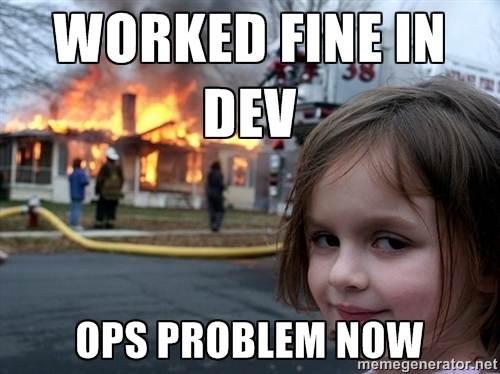
\includegraphics[width=0.45\textwidth]{images/devops.jpg}
\end{center}

This is not the case at startup companies. There isn't the money to pay for separate developers and operations teams. And in the beginning there's probably not that many servers, just a few demo systems, test systems, etc... but it spirals out from there. You're not really going to ask the sales guys to manage these servers, are you? So, there's DevOps. 

Is DevOps a good idea? Like most ideas it can be used for both good and evil. There's a lot to be said for letting the developers be involved in all the parts of the software from development to deployment to management to training the customers. Developers can learn a lot by having to do these kinds of things, and be motivated to make proper management and maintenance tools and procedures. 

There's also something to be said for never letting the developers out of their cubes and keeping them far, far away from the customers. They will be scared. Both parties.

Thanks to Chris Jones and Niall Murphy for the following points.

\subsection*{Configuration as code}
Systems have long come with complicated configuration options.
Sendmail is particularly notorious, but apache and nginx aren't super
easy to configure either.\footnote{If anyone should be foolish enough to want to look into procmail, well, good luck to you...} The first principle is to treat \emph{configuration as code}.
Therefore:
\begin{itemize}
\item use version control on your configuration.
\item test your configurations: that means that you check that they
  generate expected files, or that they spawn expected
  services. (Behaviours, or outcomes.) Also, configurations should
  ``converge''. Unlike code, they might not terminate; we're talking
  indefinitely-running services, after all. But the CPU usage should
  go down after a while, for instance.
\item aim for a suite of modular services that integrate together smoothly.
\item refactor configuration files (Puppet manifests, Chef recipes, etc);
\item use continuous builds (more on that later).
\end{itemize}

Furthermore, it's an excellent idea to have tools for configuration. It's not enough to just have a wiki page or github document titled ``How to Install AwesomeApp'' (fill in name of program here). There are tons of great tools like the Red Hat Package Manager (RPM) which will allow you to make the installation and update process automatic and simple. Complicated means mistakes... people forget steps. They are human. 

\subsection*{Servers as cattle, not pets}
By servers, I mean servers, or virtual machines, or containers.
At a certain scale (and it's smaller than you think), it's useful to
mass-produce tools for dealing with servers, rather than doing tasks
manually. At a minimum, you need to be able to set up these servers
without manual intervention. They should be able to be spun up 
programmatically.
% http://smithmeadows.com/wp-content/uploads/2012/10/Cattle.jpg

\subsection*{Common infrastructure}
Use APIs to access your infrastructure. Some examples:
\begin{itemize}
\item storage: some sort of access layer to MongoDB or Amazon S3 or whatever;
\item naming and discovery infrastructure (more below);
\item monitoring infrastructure.
\end{itemize}
Try to avoid one-offs by using, for instance, open-source tools when applicable.
Be prepared to build your own tools if needed.

\subsection*{Design for 10$\times$ growth, redesign before 100$\times$}
[original credit: Jeff Dean at Google] This discussion is based on
Martin Fowler's piece on sacrificial architecture:
\url{http://martinfowler.com/bliki/SacrificialArchitecture.html}.

Consider eBay: in 1995, perl scripts; in 1997, C++/Windows; in 2002,
Java.  Each of these architectures was appropriate at the time, but
not as the requirements change. The more sophisticated successor
architectures, however, would have been overkill at an earlier
time. And it's hard to predict what would be needed in the future.
% look up eBay growth stats
%http://martinfowler.com/bliki/images/sacrificialArchitecture/sketch.png
%http://web.archive.org/web/20000510004517/http://www.ebay.com/
% http://www.ebay.com/

\begin{quote}
``Perf is a feature''.\\
\hfill --- Jeff Atwood
\end{quote}
That is, you apply developer time to perf, and you make engineering tradeoffs
to get it. Some thoughts:
\begin{itemize}
\item design with the eventual replacement in mind;
\item don't abandon internal quality (e.g. modularity);
\item sacrifice individual modules at a time, not the whole system;
\item you can also implement new features with a rough draft and deploy to a test audience.
\end{itemize}

\subsection*{Naming}
Naming is one of the hard problems in computing. There is a saying that there are only two hard things in computers: cache invalidation, naming things, and off by one errors. 

There are a
lot of ways to name things. We'll talk about
systems/VMs\footnote{\url{http://mnx.io/blog/a-proper-naming-scheme}},
but naming is necessary for resources of all kinds.

In brief:
\begin{itemize}
\item use canonical one-word names for servers;
\item but, use aliases to specify functions, e.g. 1) geography (nyc); 2) environment (dev/tst/stg/prod); 
3) purpose (app/sql/etc); and 4) serial number.
\end{itemize}
This enables you to have a way of referring to each machine in an absolute sense, but also 
allows you to use functional names when creating dependencies between systems.

There's also the Java package approach of infinite dots: live.application.customer.webdomain.com or however you want to call it. But pick something and be consistent.

\subsection*{Other Topics}
Beyond the five principles above, there are a couple more techniques that particularly apply to
DevOps:

\paragraph{Continuous Integration.} 
This is now a best practice. It's enabled by the use of version control, good tests, and scripted deployments.
It works like this:
\begin{itemize}
\item pull code from version control;
\item build;
\item run tests;
\item report results.
\end{itemize}
What's also key is a social convention to not break the build. These things get done automatically on every commit and the results are sent to people by e-mail or instant messenger (because e-mail is for old people, right?).\footnote{I did work at a company where the person who broke the build got a sign outside his cubicle that said IOTD - Idiot of the Day. I'm not too proud to admit that I won this award on my last day of the co-op term.}

%https://jenkins-ci.org/sites/default/files/jenkins_logo.png

CI is good for all code, but it's especially good for configuration-as-code, which is especially likely
to break in different environments.

\paragraph{Canarying.}
%http://www.post-gazette.com/image/2013/10/29/ca27,76,1566,1822/Canary.jpg
Deploy new software incrementally alongside production software, also known as ``test in prod''. Sometimes
you just don't know how code is really going to work until you try it. After, of course, you use your best
efforts to make sure the code is good. Steps:
\begin{itemize}
\item stage for deployment;
\item remove canary servers from service;
\item upgrade canary servers;
\item run automatic tests on upgraded canaries;
\item reintroduce canary servers into service;
\item see how it goes!
\end{itemize}
Of course, you should implement your system so that rollback is possible.

\paragraph{Monitoring.}

Monitoring is surprisingly difficult. There are a lot of recommendations about what to monitor and what to do about it. We care about performance so here are a few things to think about:

\begin{itemize}
	\item CPU Load
	\item Memory Utilization
	\item Disk Space
	\item Disk I/O
	\item Network Traffic
	\item Clock Skew
	\item Application Response Times
\end{itemize}

With multiple systems, you will want some sort of dashboard that gives an overview of all the multiple systems in a summary. The summary needs to be sufficiently detailed that you can detect if anything is wrong, but not an overwhelming wall of data. Then you do not necessarily want to pay someone to stare at the dashboard and press the  ``Red Alert!'' button if anything goes out of some preset range of what is okay. No, for that we need some automatic monitoring.

Here's one way to think about it. 
% track down the source here: Niall Murphy interview.
\begin{itemize}
\item {\bf Alerts}: a human must take action now;
\item {\bf Tickets}: a human must take action soon (hours or days);
\item {\bf Logging}: no need to look at this except for forensic/diagnostic purposes.
\end{itemize}
A common bad situation is logs-as-tickets: you should never be in the
situation where you routinely have to look through logs to find
errors. Write code to scan logs.

It is very important to be judicious about the use of alerts. If your alerts are too common, they get ignored. When you hear the fire alarm in a building, chances are your thought is not ``the building is on fire; I should leave it immediately in an orderly fashion.''. More likely your reaction is ``great, some jerk\footnote{This is the PG-13 version of what I actually think.} has pulled the fire alarm for a stupid prank or to get out of failing a midterm.'' This is because we have been trained by far too many false alarms to think that any alarm is a false one. It's a good heuristic; you'll be correct most of the time. But if there is an actual fire, you will not only be wrong, you might also be dead.

Still, alerts and tickets are a great way to make user pain into developer pain. Being woken up in the middle of the night (... day? A lot of programmers are nocturnal, now that I think of it) because of some SUPER CRITICAL ticket OMG KITTENS ARE ENDANGERED is an excellent way to learn the lesson that production code needs to be written carefully, reviewed, QA'd, and perhaps run by a customer or two before it gets deployed to everyone. Developers, being human (... grant me some leeway here), will probably take steps to avoid their pain\footnote{There is a great quotation to this effect by Fr\'ed\'eric Bastiat about how men will avoid pain and work is pain.}. and they will take steps that keep these things from happening in the future: good processes and monitoring and all that goes with it.

\section*{Clusters versus Laptops}
There is a paper about this: Frank McSherry, Michael Isard, Derek G. Murray. ``Scalability! But at what COST?'' HotOS XV. This part of the lecture is based on the companion blog post~\cite{scalecost}.

The key idea: scaling to big data systems introduces substantial overhead. Let's just see how, say, a laptop compares, in absolute times, to 128-core big data systems.

\paragraph{Summary.} Big data systems haven't yet been shown to be obviously good; current evaluation is lacking.
The important metric is not just scalability; absolute
performance matters a lot too. We don't want a situation where we are just scaling up to $n$ systems to deal with the complexity of scaling up to $n$ systems. Or, as Oscar Wilde put it: ``The bureaucracy is expanding to meet the needs of the expanding bureaucracy.''

\paragraph{Methodology.} We'll compare a competent single-threaded implementation to top
big data systems, as described in an OSDI 2014 (top OS conference) paper on GraphX\cite{graphx}. The domain: graph processing
algorithms, namely PageRank and graph connectivity (for which the bottleneck is label propagation). The subjects: graphs with billions of edges, amounting to a few
GB of data.

\paragraph{Results.} 128 cores don't consistently beat a laptop at PageRank: e.g. 249--857s on the twitter\_rv dataset for the big data system vs 300s for the laptop, and they are 2$\times$ slower for label
propagation, at 251--1784s for the big data system vs 153s on
twitter\_rv. From the blogpost:

\begin{center}
	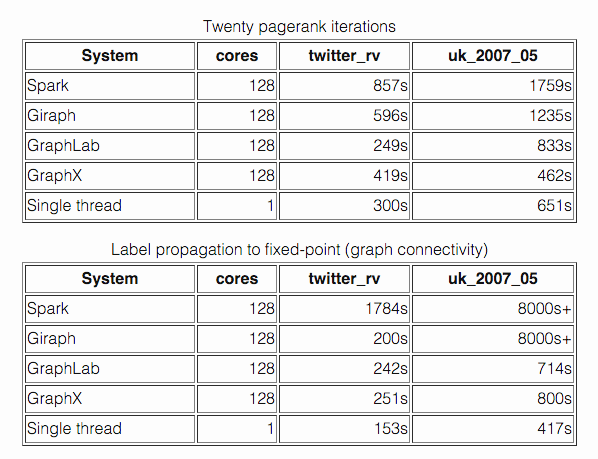
\includegraphics[width=0.60\textwidth]{images/pagerank.png}
\end{center}

\paragraph{Wait, there's more.} I keep on saying that we can improve algorithms for additional performance boosts too.
But that doesn't generalize, so it's hard to teach. In this case, two improvements are: using Hilbert curves
for data layout, improving memory locality, which helps a lot for PageRank; and using a union-find algorithm 
(which is also parallelizable). ``10$\times$ faster, 100$\times$ less embarrassing''.  We observe an overall
$2\times$ speedup for PageRank and $10\times$ speedup for label propagation.

\paragraph{Takeaways.} Some thoughts to keep in mind, from the authors:
\begin{itemize}
\item    ``If you are going to use a big data system for yourself, see if it is faster than your laptop.''
\item    ``If you are going to build a big data system for others, see that it is faster than my laptop.''
\end{itemize}






\bibliographystyle{alphaurl}
\bibliography{459}


\end{document}